% 本文件是示例论文的一部分
% 论文的主文件位于上级目录的 `bachelor.tex` 或 `master.tex`

\chapter{绪论}
\section{磁悬浮电机概述}
轴承是旋转机械中必不可少的组件之一。传统机械轴承依靠滚珠结构支撑转子,该结构经过长期的发展和研究已经取得较高的精度和可靠性。然而在高速透平机械领域,传统机械轴承的应力和摩擦力问题往往使得其支撑的转子转速不能过高,由此难以广泛应用;在医疗行业中,无菌环境对仪器设备的清洁性要求十分严格,机械轴承需要定期添加润滑剂维护的特性不利于其在此种场合下的应用。与此形成对比的是磁悬浮轴承技术。磁悬浮轴承使用磁力将转子吸引在轴承中心,定子(轴承)与转子之间无物理接触。由此使得轴承中不再有应力和摩擦力问题,磁轴承可以支撑转子更高速运转。同时因为定子与转子无接触,磁悬浮轴承也无需使用润滑剂。因而具有无菌或清洁场合应用的优势。此外与传统机械轴承不同的是,磁悬浮轴承通过主动控制的方式支撑转子,因而传统机械轴承中通常设计完成即固定的属性,如轴承刚度、轴承阻尼等,在磁悬浮轴承中可以主动调节,以适应不同场合转子的动力学要求。本文将采用磁悬浮轴承的电机统称为磁悬浮电机。磁悬浮轴承的无摩擦、无需润滑、寿命长以及动力学特性可调节的优点,使得工业领域出现多种类型的磁悬浮电机,如磁悬浮分子泵、磁悬浮离心机、磁悬浮压缩机等。

磁悬浮电机的典型应用之一是磁悬浮空气压缩机。空气压缩机是一种把空气进行压缩、将低压气体变为高压气体,然后输送给其他设备的机械装置。针对各种工业生产设备而言,其目的是为气动设备、气力输送设备、高温检测设备及清扫设备提供一定压力、流量、湿度和温度的气源。它是空气分离系统的“心脏”部分,也是分离设备接受原料空气的前置装置。

空气压缩机已经普遍应用于矿山、化工、制冷、机械、交通运输、国防科技等重要行业,也逐渐发展成为各行业动力源头,成为各企业设备中的核心装置之一。由生命周期评价理论分析,空气压缩机的整体运行成本由初始采购成本、维护保养成本和能源运行成本组成,在这当中初始采购成本仅占10\%左右,而能源消耗成本却高达75\%。在大多数生产企业中,生产压缩空气的能源消耗大约占全部电力消耗的 10\%-30\%。空气压缩机的比功率和气流量等的参数设置均会影响其运行效率,而另一个重要的能源消耗是空气压缩机的转子和机械轴承的摩擦带来的能量流失、机械零部件消耗以及润滑材料的损耗。

目前的空气压缩机大部分采用机械轴承,此类轴承系统存在以下问题:一、高速转子和机械轴承之间需要设计良好的油路进行润滑和冷却;二、由于机械轴承的最大应力限制,空气压缩机的转速无法达到理想的高速或超高速水平;三、电机转子的质量分布不平衡引起振动力,加剧噪声同时加速机械轴承磨损。机械轴承存在的以上弊端降低了空气压缩机的性能,增加了空气压缩机的结构复杂度,同时增加了系统的功耗以及维护和运行成本。磁悬浮空气压缩机即可借助磁力控制的优势,无接触地支撑转子高速旋转,并可通过主动振动控制技术消除电机转子质量分布不平衡带来的不利影响。

\section{磁悬浮轴承研究现状}
磁悬浮轴承是利用磁场力使定子与转子之间无接触的一种新型轴承。相比于传统机械轴承,磁悬浮轴承具有以下优良特性:一、无接触、无需润滑以及无磨损的特性使得轴承损耗大幅降低,且更适合恶劣工况;二、磁轴承支承的转子工作转速仅受限制于转子的材料,从而可以达到较高水平;三、通过应用不同的控制律即可获得不同的轴承的动力学性能,达到动态调整轴承的承受负载能力的目的。

按照轴承力的来源,电磁轴承可以分为三类:被动式磁轴承(PMB:Permanent Magnetic Bearing)、主动式磁轴承(AMB:Active Magnetic Bearing)、混合式磁轴承(HMB:Hybrid Magnetic Bearing)。被动式磁轴承的轴承力仅来源于永久磁铁,由于其固有阻尼极低,所以被动式磁轴承的工业应用范围较小;主动式磁轴承包含铜线圈或其他主动控制单元,可根据控制目标的变化实时调节电磁力的大小,同时由于电磁铁的磁场力可控,磁场力的动态特性方便调节,所以主动式磁轴承的应用范围较广;混合式磁轴承又称作永磁偏置磁轴承,其磁场力由永磁体产生的偏置磁场和受控的电流共同作用产生。混合式磁轴承的开关功放的功率更小,损耗更低,这使得混合式磁轴承布局紧凑、效率更高。

关于磁悬浮轴承的研究可以追溯到1842年英国科学家Earnshaw,他通过理论证明了铁磁体不可能仅由另一个永久磁铁支承而在六个自由度上都保持自由、稳定的悬浮,必须至少有一个自由度被机械或其它约束所消除\cite{earnshaw1842nature}。直到一百年后第二次世界大战曼哈顿计划中,美国弗吉尼亚大学的Jesse Beams才将磁悬浮技术首次应用在提取同位素的离心机上。1937年,德国工程师Kemper申请了一项磁悬浮轴承的专利\cite{kemper1937schwebebahn},这正是稍后出现的磁悬浮列车的前身。1957年,法国的Hispano-Suiza公司第一次提出了使用传感器与电磁铁组成主动悬浮的想法\cite{patent19571186527}。1969年,德国高速单轨磁悬浮列车公司Transrapid开始进行磁悬浮列车实验。1976年,瑞典SKF公司和法国SEP公司一起投资成立S2M公司,标志着磁悬浮技术正是开始走向商用阶段。1981年,S2M公司在Hanover欧洲国际机床展览会上推出B20/500磁浮主轴系统,转子转速35000转/分。1983年,德国Transrapid公司展出磁悬浮列车Transrapid 06,时速406KM。1983年,搭载于美国航天飞机的欧洲空间实验舱内安装的真空泵采用了电磁轴承。1986年,法国将姿态控制用的磁浮飞轮安装在SPOT地球观测卫星上。1990年,瑞士联邦工学院研制成AMB铣削电主轴切削速度达6000转/分\cite{siegwart1990design}。同年,日本研制超高速内圆磨电主轴,转速达180000转/分\cite{ota1990monitoring}。1997年,日本Terumo公司、NTN公司和Setsunan University大学研究团队在成年羊体内移植人造心脏泵,羊存活时间超过一年\cite{nojiri1997more}。2002年,德国Incor公司在人体内首次应用心脏泵,24名患者移植磁悬浮心脏泵,患者30天存活率达79\%\cite{hetzer2004first}。2003年,美国Levitronix Centrimag在18名患者体内移植了磁悬浮心脏泵,患者30天存活率达50\%,术后两年内器件未出现故障\cite{de2006clinical}。

国内对磁悬浮技术的研究始于20世纪90年代。1988年,长沙国防科技大学杨泉林尝试使用状态空间法进行磁悬浮轴承控制器的参数设计\cite{杨泉林1988状态反馈去耦原理在磁悬浮轴承设计中的应用},仿真效果良好,但是未进行实验验证。1992年,西安交通大学李黎川提出使用电流作为控制量以降低系统阶数,理论分析表明非线性程度可以得到大幅改善\cite{李黎川1992磁悬浮轴承物理模型的降阶及非线性改善}。1996年,哈尔滨工业大学赵雷对磁悬浮轴承中的磁悬浮力建模、非线性力控制问题做了诸多研究\cite{赵雷1996可控磁悬浮轴承刚度的提高与大范围稳定性,赵雷1996径向磁悬浮轴承结构特性研究及其模型的建立}。1998年,北京工业大学黄晓蔚率先开始对数字化磁轴承控制系统的研究,实现16kg转子12000转/分的稳定运转\cite{黄晓蔚1998数字控制的有源磁悬浮轴承的实验研究}。1999年,清华大学丛华研究了磁悬浮轴承控制系统中的电涡流传感器的模型和设计方法,提高了位移传感器的带宽\cite{丛华1999电涡流传感器动态响应特性研究}。2000年后,国内磁悬浮轴承的研究呈现较大的发展。清华大学对磁悬浮轴承和刚度和阻尼等参数做了诸多深入的研究\cite{赵雷1999可控磁悬浮轴承刚度与阻尼特性研究}。南京航空航天大学研究磁悬浮轴承的结构设计,提出多种混合磁悬浮轴承设计方案,并将其应用在多种类型的电机上\cite{朱熀秋2002永磁偏置径向,曾励1999永磁偏置的混合磁悬浮轴承的研究}。武汉理工大学关注磁悬浮控制系统的控制方法研究,如变参数PID控制、模糊控制\cite{苏义鑫2004磁悬浮轴承的变参数,刘晓军2006人工心脏泵磁悬浮转子非线性特性及控制方法研究}。上海大学研究了磁悬浮轴承在机床主轴中的应用,转子稳定运行转速达到8000转/分\cite{张钢2005磁悬浮支承技术在机床中的应用}。哈尔滨工业大学设计磁悬浮结构,将其应用于分子泵中\cite{周红海2006分子泵磁悬浮轴承结构及功率放大器设计}。山东大学针对人工心脏泵提出了多种磁悬浮应用方案\cite{关勇2010轴流式磁悬浮人工心脏泵磁悬浮轴承系统设计,杨晟2010轴流式磁悬浮人工心脏泵驱动电机的研究}。

学界磁悬浮轴承主题会议有国际磁悬浮轴承会议(ISMB:International Symposium on Magnetic Bearings)和中国磁悬浮轴承会议(CSMB:Chinese Symposium on Magnetic Bearings)。前者自1988年开始,每两年举办一次,至2019年已成功举行了十六届。后者自2005年开始,每两年举办一次,至2019年已成功举行了七届。定期举行的会议为世界各地的磁悬浮技术研究学者提供了学术交流的平台,大幅促进了磁悬浮技术的发展。

工业领域磁悬浮技术已经成熟发展。瑞士Mecos公司、美国Calnetix公司和Waukesha公司、瑞典的SKF公司、加拿大的REVOLVE公司、法国的S2M公司(现已被SKF收购)、德国的LEViTEC公司、芬兰的High Speed公司、俄罗斯的OKBM和日本的精工在磁悬浮的商业应用上占据主流市场地位。\autoref{fig:industrial_amb}是Mecos公司2019年在售产品二氧化碳鼓风机,二氧化碳用作某些新能源发电场合的冷却介质,二氧化碳鼓风机用于产生高速气流。该鼓风机电机功率15kW,稳定运行速度可达54000转/分。Calnetix公司的余热回收发电系统如\autoref{fig:industrial_amb}所示,其中磁悬浮发电机发电功率可达125kW,电机转速可达26500转/分。SKF公司为污水处理厂通用鼓风机系统提供75至350kW功率的磁悬浮无油电动机解决方案如\autoref{fig:industrial_amb}所示,其电动机转子转速可达40000转/分,转子位移采集频率可达15kHz。

\begin{figure}[H]
  \subfloat[Mecos公司二氧化碳鼓风机]{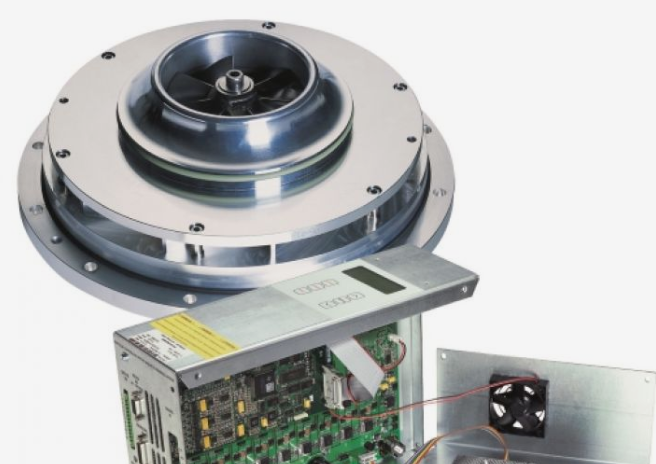
\includegraphics[width=6cm]{1-Mecos.png}}\quad
  \subfloat[Calnetix公司余热回收发电系统]{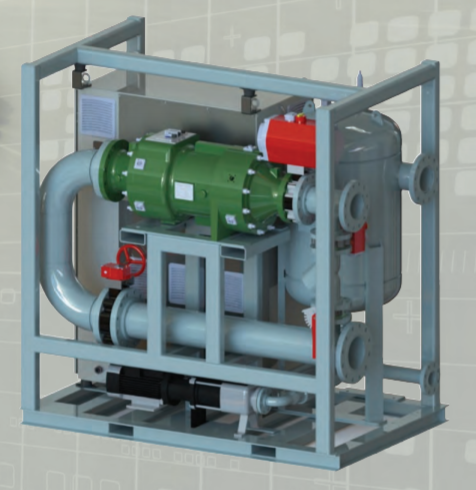
\includegraphics[width=6cm]{1-Calnetix.png}}\quad
  \subfloat[SKF公司污水处理厂通用鼓风机系统]{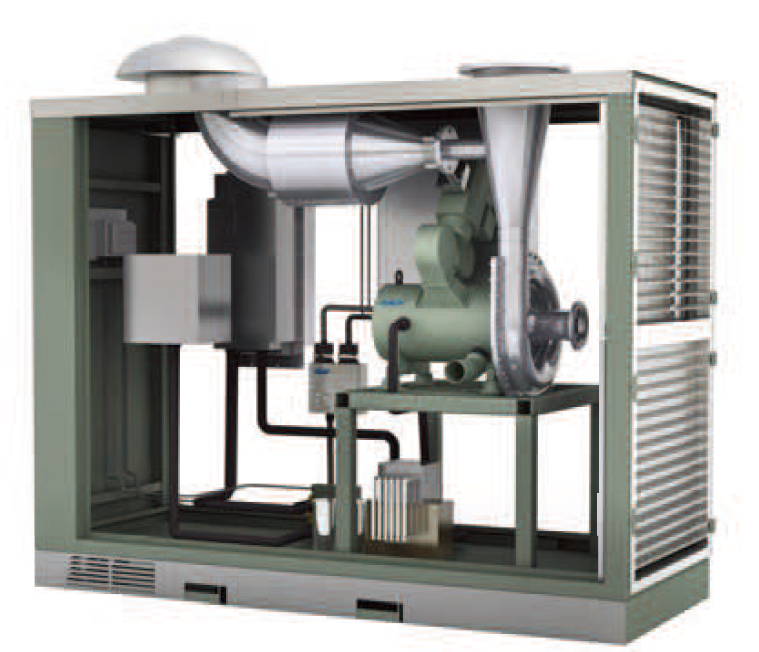
\includegraphics[width=6cm]{1-Skf.png}}\quad  
  \caption[国外磁悬浮电机的应用]{国外磁悬浮电机的应用\label{fig:industrial_amb}}
\end{figure}

国内磁悬浮轴承技术商用成熟的公司有天津飞旋科技和南京磁谷科技,分别由清华大学和南京航空航天大学的技术团队创立。飞旋目前已经研发出磁悬浮复合分子泵、磁悬浮离心鼓风机等产品。磁谷科技的磁悬浮离心式鼓风机进口流量可达280立方米/分,已应用在多种场合。上述产品如\autoref{fig:industrial_amb}所示。国内磁悬浮电机市场正处于高速发展时期,如何将学术界的研究成果转换应用在工业领域,充分发挥磁悬浮技术的节能、清洁优势,是目前行业中共同致力解决的问题。

\begin{figure}[H]
  \subfloat[飞旋科技磁悬浮复合分子泵]{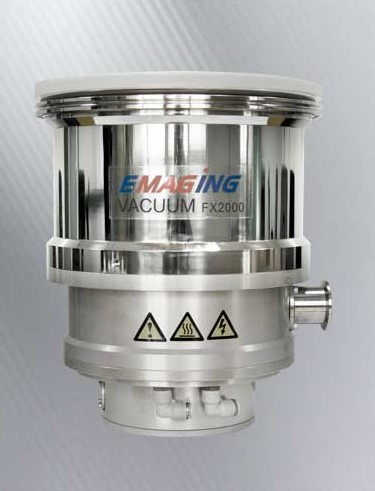
\includegraphics[width=6cm]{1-Feixuan.jpg}}\quad
  \subfloat[磁谷科技磁悬浮离心式鼓风机]{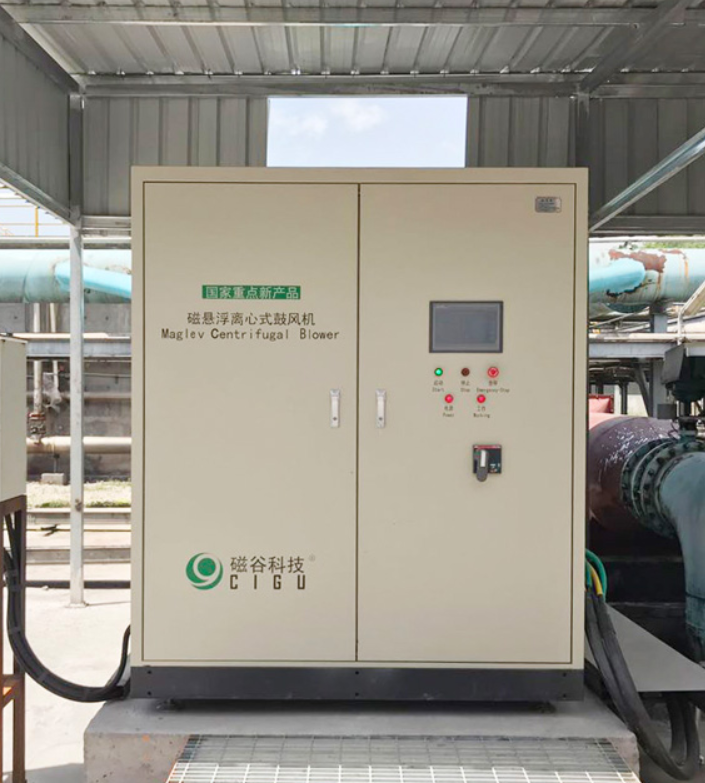
\includegraphics[width=6cm]{1-Cigu.png}}\quad
  \caption[国内磁悬浮电机的应用]{国内磁悬浮电机的应用\label{fig:industrial_amb_cn}}
\end{figure}

\section{磁悬浮振动控制技术研究现状}
理想情况下,转子位于平衡位置绕几何轴旋转,控制绕组电流无周期分量,转子不受到周期性波动的磁场力作用。而实际系统中,电流中往往含有周期分量,导致磁轴承对转子施加周期性磁场力,进而使基座受到同频反作用力,产生振动力。此振动力来源来自转子质量不平衡、传感器偏差和磁极偏差。转子质量不平衡是指由于机械加工的工艺限制,转子的几何轴和惯性轴不重合,由此是的旋转轴介于几何轴和惯性轴之间,引起与转速同频的振动力;传感器偏差是指被传感器检测的转子表面为非理想圆形,且检测面材料不均匀会在测量得到的位移信号中引入同频或者倍频信息,引起同频或倍频振动力;磁极偏差是指径向磁极对称中心与转子旋转中心不重合,该因素影响较小,通常可忽略不计。

磁轴承的不平衡控制目标有三类。第一类是实现零电流控制:控制线圈电流为交流分量为零,则系统可以实现最低电力功耗,但是残余的位移刚度仍会引起部分残余的不平衡振动力;第二类是实现零力控制:控制磁轴承电磁力的交流分量为零,此状态下可以实现最低振动力为零,但是此时线圈电流交流分量幅值不为零;第三类是零位移控制:控制转子的旋转轴与几何轴重合,达到高回转精度的要求,但是会加剧振动力。

第一类和第二类控制目标适用于动力传动领域,如鼓风机或压缩机,此类应用场合往往对转子的回转精度要求不高,而要求整机功耗或振动力越小越好;第三类控制目标适用于机械加工领域,如机床加工电主轴,此类应用场合要求转子具有非常高的回转精度,以满足高精度加工需求。磁悬浮空气压缩机转速高、功耗大,控制目的是降低功耗以及降低振动,因此本文的不平衡振动的控制目标是第一类或第二类。

实际工作状况下, 磁悬浮轴承支承的空气压缩机转子在额定转速范围内高速旋转,转子不平衡带来的振动大幅增加了系统的功耗、降低了系统的稳定性,并且带来的噪声污染问题。因此,研究如何抑制磁悬浮轴承振动具有重要意义。

磁悬浮轴承中的振动主要来源是转子质量不平衡和传感器误差。由于转子加工精度限制,其内部质量分布总是会存在一定程度的质量不平衡。该不平衡质量引入与转子转速同频的正弦扰动信号。传感器误差是指位移传感器检测面不均衡,由此导致位移信号中包含转子转速同频已经倍频的正弦扰动信号。质量不平衡和传感器误差使得控制控制电流中存在谐波成分,引起磁悬浮轴承中的磁悬浮振动力。

许多文献针对磁悬浮轴承中的同频振动问题做了深入研究。1983年,Burrows通过开环控制的方式抑制转子不平衡位移响应,实现不平衡补偿,该方法依赖于转子不平衡响应数据以及影响矩阵T\cite{burrows1983vibration}。1989年,Burrows在他之前的研究基础上加入自适应环节,实现最优矢量自动更新\cite{burrows1989active}。1993年,Knospe在Burrows方法的基础上采用自适应方法,进一步研究了影响系数矩阵T在线生成\cite{knospe1993adaptive}。1994年,N., Taguchi提出自适应反馈补偿方法自动平衡或不平衡补偿,同频补偿信号注入到控制回路中实现零位移或者零力控制,该方法的缺点是无法从理论上证明收敛性\cite{taguchi1994unbalance}。1995年,Mohamed提出使用Q-parameterization方法实现自动平衡\cite{mohamed1995imbalance}。1996年,Herzog提出通用陷波器实现自动平衡,该方法基于闭环系统设计,且通过测量系统的灵敏度函数、无需精准的系统参数模型,具有参数设计流程简单,且可以保持原闭环系统的稳定性的优点,该方法后被广泛引用并研究\cite{herzog1996unbalance}。1996年,Matsumura使用H无穷控制策略实现自动平衡\cite{matsumura1996application}。1997年,HS Na在不改变环路的稳定性的条件下,插入LMS滤波器抑制不平衡振动位移,实现不平衡补偿\cite{na1997adaptive}。1998年,Nonami提出了一种不依赖系统传递函数全部信息的控制方法这是一种尝试-调整方法,该方法能找到正确的同频控制电流相角。虽未给出理论证明,但通过大量仿真研究表明了其有效性与收敛性\cite{nonami1998unbalance}。1999年,Nonami等将他的上一篇文章的方法进一步发展, 以同时抑制同频振动及倍频振动\cite{nonami1999adaptive}。2002年,Markert论述了迭代搜索算法用于自适应抑制转子不平衡响应, 通过对同频控制电磁力与相应位移响应的迭代搜索, 可在不清楚转子系统模型情况下实现AMB力控制,但仅对简单系统模型起作用。对复杂超临界挠性转子,他们设计了基于精确系统模型的算法, 基本思想仍然是基于电磁力到位移检测点的传递函数, 反算所需同频控制力。使用该方法,Markert在一挠性轴上实现了转子平稳超临界运转,临界频率处的不平衡响应在控制力作用下减小了90\%\cite{markert2002unbalance}。2002年,J.Shi采用最小均方( LMS,Least Mean Square) 算法:通过产生等增益、反相位的同频信号,前馈补偿同频电流,实现同频电流刚度力消除,但该方法未考虑位移刚度力产生的振动,且因LMS算法步长固定,无法兼顾系统稳定性及收敛速度要求,仅适用某特定转速范围,实现自动平衡\cite{shi2002direct}。2004年,J.Shi使用自适应方法实现自动平衡,控制器的稳定性是靠不断更新参数来实现的\cite{shi2004synchronous}。2005年,Chao使用时域迭代学习控制和增益调度方法,实现自动平衡,它使用跟随转速变化学习周期和学习增益来达到系统的稳定\cite{bi2005automatic}。2006年,Matras引入模型参考自适应方法, 可解决MIMO耦合问题。其基本思想是令一扰动输入的对象, 通过自适应方法跟踪一无扰动输入的参考模型, 以抑制对输入扰动的响应。仿真与实验结果证明, 对频率已知、持续稳定的正弦激励, 即便幅值未知、且随时间发生改变, 该方法仍有效。缺点是在应用过程中,参数中的权重阵选取很关键, 且算法收敛速度较慢\cite{matras2006suppression}。2006年,彭晓军认为1996年通用陷波器设计未考虑“低阻尼振荡现象”,他提出约束条件更加严格的通用陷波器设计方法\cite{彭晓军2006磁电轴承中抑制不平衡振动的陷波滤波器设计方法}。2007年,Vahedforough提出改进的自适应不平衡控制方法,他采用两个自适应观测器,实现自动平衡\cite{vahedforough2007estimation}。2012年,Xu提出了一种基于相移通用陷波反馈控制的同频电流抑制方法,可有效抑制控制器、功放系统产生的同频电流,实现自动平衡\cite{xu2012stability}。2014年,缪存孝在2012年Xu的研究基础上,考虑感应电动势,抑制同频电流\cite{缪存孝2014含转子不平衡的磁轴承建模与同频电流抑制}。2015年,崔培玲采用相移陷波器,以同频振动力为控制目标,消除同频振动力,实现自动平衡\cite{崔培玲2015基于相移陷波器的磁轴承不平衡振动全频自适应控制}。2016年,Peng提出谐振控制器解决传统控制策略不是针对时变转速的问题,以及针对时变转速但是控制器结构复杂的问题,该方法补偿掉位移负刚度,实现自动平衡\cite{peng2016synchronous}。2017年,Peng提出使用多谐振控制器抑制基波和谐波电流,实现自动平衡\cite{peng2016frequency}。

另一方面,针对位移传感器引入的倍频扰动问题,亦有许多文献做了相关的研究。第一类控制方法是将多个针对单一频率的振动控制器连接在一起。Mahdi Darbandi将多个陷波器组合来消除谐波电流,同时根据系统的灵敏度函数曲线来设计陷波器参数,以保证闭环系统稳定性\cite{mahdi2017harmonic}。然而,当需要一直的谐波频率数量较多时,需要组合多个陷波器,由此使得计算负担迅速加大。重复控制器具有单路结构消除多种频率扰动的能力,适合谐波抑制场合。重复控制器早期应用于电源系统中以消除跟踪误差\cite{zhou2008plug},Xu将重复控制器应用在磁悬浮轴承控制中,消除了控制电流中的谐波成分\cite{xu2015model}。Cui改进了重复控制器的结构,将重复控制器的低通滤波器移动至延时环路之外,由此得到了更好的电流谐波抑制效果\cite{cui2016suppression}。Zhou提出奇数次重复控制器的应用方法,其应用场合是PWM变换器\cite{zhou2006zero}。但磁悬浮轴承是开环不稳定结构,奇数次重复控制器不能直接从PWM变换器移植到磁悬浮轴承的控制回路中。如何在磁悬浮轴承中应用重复控制器——理论推导、稳定性分析、参数设计仍是有待深入研究的问题。

除上述提到的针对同频和倍频扰动的主控抑制方法,还有使用动平衡技术的被控抑制方法。主动振动抑制方法无法同时实现零电流或者零位移控制,这是因为闭环控制之下,无法通过调节控制器参数同时实现减小轴承刚度和增大轴承刚度。动平衡技术消除不平衡质量,可以从源头上除去同频扰动,进而达到既抑制电流同频成分,又抑制位移同频成分的目的。传统的动平衡借助动平衡机完成,需要将电机转子单独放置在动平衡机上,通过增重或去重完成动平衡之后再装回电机。然而磁悬浮轴承中,动平衡机的轴承系统与磁悬浮电机的轴承系统不一定重合,由此引入误差。导致即使在动平衡机上达到了良好的动平衡效果,转子在工况下旋转时,仍有一定的不平衡质量。借助磁悬浮可主动控制的特性,磁悬浮电机的转子动平衡过程可以在电机本体内完成,无需拆装转子,此过程称之为现场动平衡。影响系数法和模态平衡法是比较常用的方法之一,影响系数法是基于假设控制系统是线性的前提,通过多轮试重得到校正质量\cite{john2009relationship,ranjan2019application}。模态平衡法是先构建转子的有限元模型,然后通过实际的振动响应曲线来校正有限元模型。这两种方法的缺点是都需要多轮试重和振动响应测试\cite{wang2014field}。为了简化动平衡操作过程、降低时间消耗,近年来一些文献相继提出多种无需试重的现场动平衡方法。该方法可分为两大类:一、抑制不平衡振动位移,使转子旋转轴趋于几何轴,通过转子的控制电流辨识不平衡质量矢量\cite{fang2013field,liu2015field}。二、抑制不平衡振动力,使转子旋转轴趋于惯性轴,通过转子的位移辨识不平衡质量矢量\cite{xu2015field}。上述控制方法均需要抑制电流或位移中的交流分量,以达到控制转子旋转轴的目的。然而,以上文献仅关注了同频扰动成分的抑制,没有考虑倍频扰动成分的抑制。由此使得现场动平衡方法对不平衡质量的辨识结果精度有限。

\section{本文的研究工作和安排}
本文以抑制磁悬浮轴承系统中振动力为控制目标,分析了磁悬浮轴承系统的控制原理和振动模型,提出了两种新的振动控制方法,并在磁轴承数字控制平台上完成仿真和实验验证。本文具体的研究内容安排如下:

第一章介绍了磁悬浮电机的发展和应用现状,以空气压缩机为例阐述了磁悬浮轴承与传统机械轴承相比所具有的巨大优势。分析了国内外对磁悬浮轴承技术的研究发展。对不平衡振动抑制方法、重复控制器和现场动平衡技术的研究现状做了详尽的分析。

第二章研究了磁悬浮系统的工作原理,建立了磁悬浮轴承支撑的刚性转子动力学模型,并建立了考虑质量不平衡和传感器位移误差在内的磁悬浮系统的振动模型。

第三章提出了使用重复控制器进行主动振动控制的方法。分析了重复控制器的原理和应用背景。针对磁悬浮轴承控制场景,本文提出一种零相移奇数次重复控制器,阐述了稳定性分析方法和参数设计步骤,仿真结果验证了提出的零相移奇数次重复控制器的有效性。

第四章提出了基于现场动平衡的振动控制方法。简单分析了目前文献中的两种主流磁悬浮轴承支撑的转子现场动平衡技术。针对谐波抑制的研究空白,本人提出考虑谐波抑制的现场动平衡技术,进行了原理的推导和验证。

第五章研究了磁悬浮轴承数字控制平台的实验方案设计。介绍了硬件模块和软件设计流程,包括软件主要组成部分的设计。进行了系统特性函数——灵敏度函数的测定实验、基于零相移奇数次重复控制器的振动抑制实验和基于现场动平衡的振动抑制实验,以此验证了前文所提出算法的有效性。

第六章总结了全文的研究内容,提出了下一步的工作展望。

\chapter{磁悬浮系统和振动模型}
本章分析了磁悬浮轴承系统的硬件结构和软件控制原理。在分析磁悬浮转子动力学模型时将转子视为刚体,建立径向四自由度的广义坐标系模型。考虑质量不平衡和传感器误差因素,分析并建立了转子振动模型。

\section{磁悬浮系统工作原理}
本文研究的磁悬浮电机为磁悬浮离心压缩机。磁悬浮离心压缩机将空气进行压缩、把低压气体变为高压气体,然后输送给其他设备的机械装置。它是由一个永磁同步电机和分立在两端的两台轴向径向磁轴承组成。结构如\autoref{fig:2-1-structure}所示。该磁悬浮离心压缩机的电气参数如\autoref{tab:motor_para}所示。转子额定转速远低于其一阶弯曲频率,因此可以转子视为刚性转子,不考虑其柔性状态。

\begin{figure}
	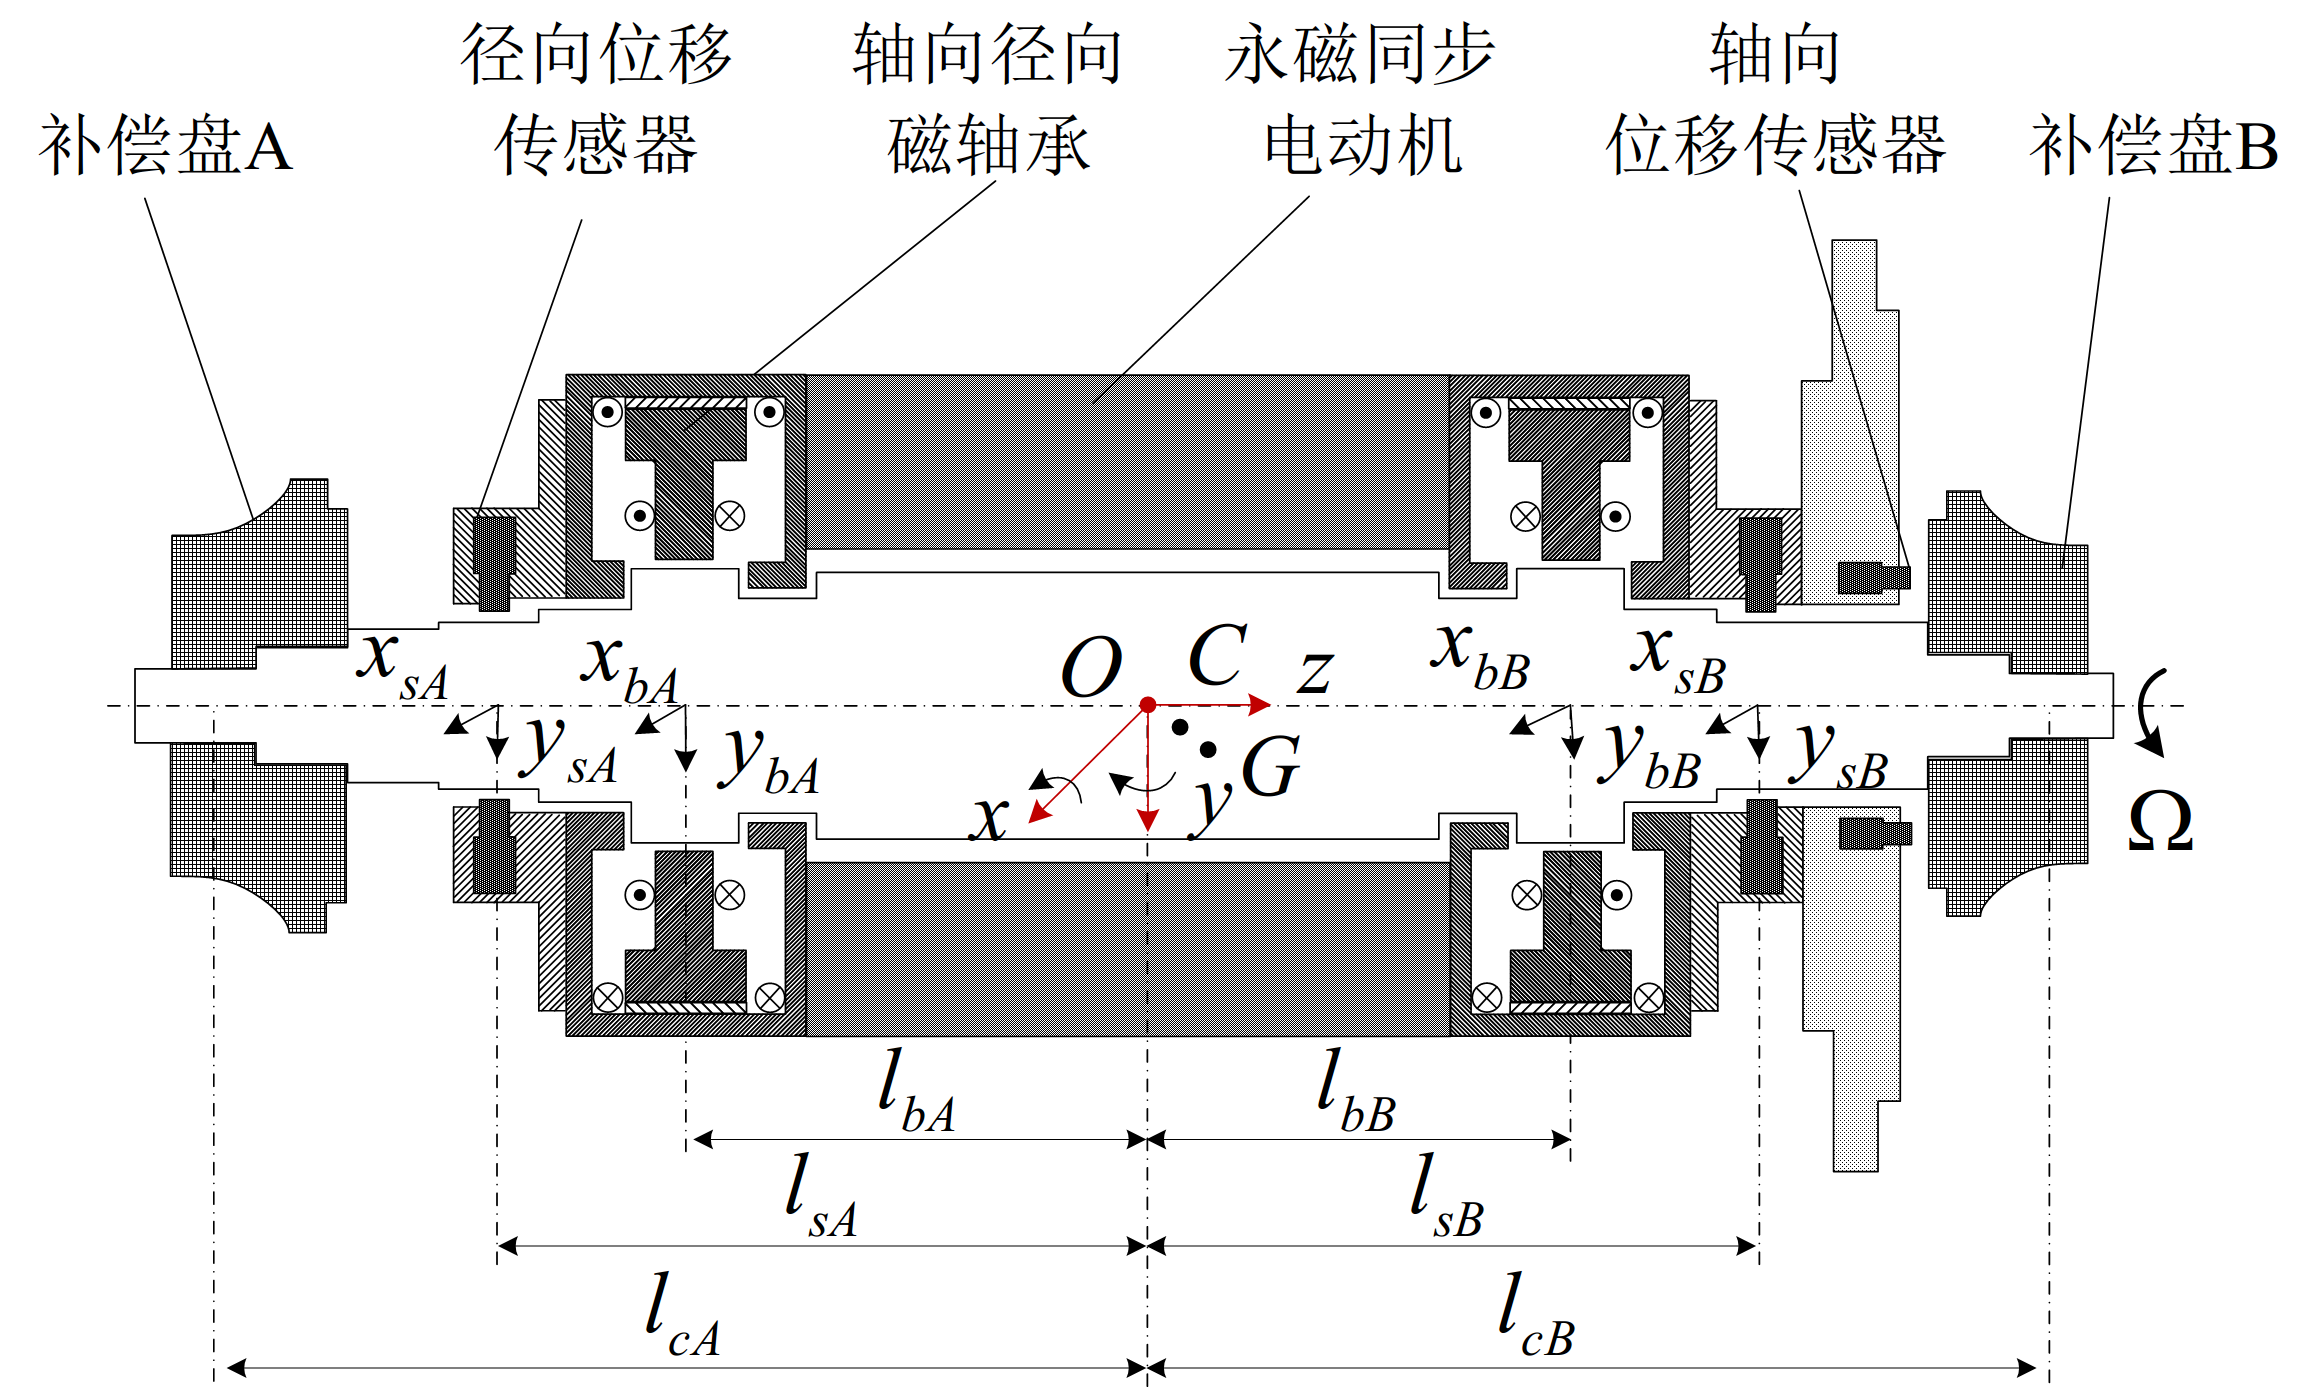
\includegraphics[scale=1.0]{2-1-structure.png}
	\caption{磁悬浮离心压缩机结构示意图}
	\label{fig:2-1-structure}
\end{figure}

\begin{table}[htb]
  \caption[磁悬浮离心压缩机电气参数]{磁悬浮离心压缩机电气参数\label{tab:motor_para}}
  \begin{tabular}{cc}
    \toprule
    物理量 & 值 \\
    \midrule
    额定功率 & 7.5kW\\
    额定转速 & 50000rpm\\
    转子一阶弯曲频率 & 1589Hz\\
    \bottomrule
  \end{tabular}
\end{table}

笛卡尔坐标系下,空间中的刚体存在六个方向上的运动:三个坐标轴方向上的平动以及绕三个坐标轴的转动,称之为六个自由度。磁悬浮离心压缩机中,两端组合的轴向径向磁轴承可以约束转子其中五个自由度的运动,余下一个自由度的转动由电机驱动器控制。

磁悬浮轴承控制的目标是使转子稳定悬浮在磁轴承中心,不与保护轴承接触。由于磁轴承和转子组成的系统是一个开环不稳定的控制系统,需要引入闭环控制才能使其保持稳定。磁悬浮轴承控制系统通常由数字信号处理器、位移传感器和功率放大器组成。

位移传感器实时高频采集转子位置,采样频率可达100kHz。高灵敏度、线性度和足够的带宽是传感器实时可靠获取转子位置的必要保障。通常位移传感器信号经降噪滤波等调理电路处理后输入到数字信号处理器中。

常用的数字信号处理器有DSP(Digtal Signal Processor),如TMS320F28335。近年来以Cortex-M4为核心的单片微处理器亦配备充足的计算能力,如STM32F4系列单片机。数字信号处理器是磁轴承控制系统的枢纽,其根据位移传感器采集的信号,向下级输出给定磁悬浮力。高速的运算能力保证各类控制算法如PID调节器、滤波器等的稳定运行。

功率放大器和磁轴承线圈共同组成磁轴承系统的执行元件。变化的转子位置将使数字信号处理器输出不同的给定电流,给定电流经功率放大器调理之后,在磁轴承线圈中产生控制电流,进而输出磁悬浮力控制转子的位置。

\section{磁悬浮转子动力学模型}
\autoref{fig:2-1-structure}中,记转子的几何中心为$ G $,质量中心为$ C $,$ l_{bA} $和$ l_{bB} $表示A端和B端轴向径向磁轴承到转子几何中心的距离,$ l_{sA} $和$ l_{sB} $表示A端和B端位移传感器到转子几何中心的距离。以磁轴承中心为原点建立广义坐标系$ O-xyz $,原点记为$ O $。转子绕$ x $和$ y $轴的旋转角度分别记为$ \alpha $和$ \beta $。转子的旋转速度记为$ \Omega $。

定义转子质量中心$ C $在$ O-xyz $中的运动位移为${\textbf{\textit{q}}_i} = {\left[ {{\beta _i},{x_i}, - {\alpha _i},{y_i}} \right]^T}$,转子几何中心$ G $在$ O-xyz $中的运动位移为${\textbf{\textit{q}}_g} = {\left[ {{\beta _g},{x_g}, - {\alpha _g},{y_g}} \right]^T}$,转子在两端位移传感器截面处的位移记为${\textbf{\textit{q}}_s} = {\left[ {{x_{sA}},{x_{sB}},{y_{sA}},{y_{sB}}} \right]^T}$,转子在两端磁轴承截面处的位移记为${\textbf{\textit{q}}_b} = {\left[ {{x_{bA}},{x_{bB}},{y_{bA}},{y_{bB}}} \right]^T}$。

由于转子在$ O-z $轴上的平动与$ O-x $和$ O-y $上的运动可视为解耦,因此轴向运动与径向运动可分开控制。本小节研究转子在径向上的动力学模型。$ \textbf{\textit{q}}_{b} $,$ \textbf{\textit{q}}_{g} $和$ \textbf{\textit{q}}_{s} $可以通过线性变换互相得到:
\begin{equation}
\label{eq2-1}
{\textbf{\textit{q}}_b} = {\textbf{\textit{B}}^T}{\textbf{\textit{q}}_g}
\end{equation}
\begin{equation}
\label{eq2-2}
{\textbf{\textit{q}}_s} = \textbf{\textit{C}}{\textbf{\textit{q}}_g}
\end{equation}
其中,
${\textbf{\textit{B}}} = \left[ {\begin{array}{*{20}{c}}
{ - {l_{bA}}}&{{l_{bB}}}&0&0\\
1&1&0&0\\
0&0&{ - {l_{bA}}}&{{l_{bB}}}\\
0&0&1&1
\end{array}} \right]$,
${\textbf{\textit{C}}} = \left[ {\begin{array}{*{20}{c}}
{ - {l_{sA}}}&{1}&0&0\\
{l_{bB}}&1&0&0\\
0&0&{ - {l_{bA}}}&{1}\\
0&0&{l_{bB}}&1
\end{array}} \right]$。

磁悬浮轴承中的磁悬浮力取决于定子和转子之间的磁场强度,而磁场强度与线圈电流和气隙长度相关,磁悬浮力$ {f_m} $可以通过转子位移和线圈电流线性表示为
\begin{equation}
\label{eq2-3}
{f_m} = {k_s}x + {k_i}i
\end{equation}
其中${k_s}$为位移刚度,${k_i}$为电流刚度。由于本文研究的磁悬浮离心压缩机中的磁悬浮轴承是对称设计结构,因此两端的三自由度磁悬浮轴承的位移刚度和电流刚度是一样的,即$ks_A = k_{sB} = k_s$,$k_{iA} = k_{iB} = k_i$。根据牛顿运动定律,转子的动力学方程即可以表示为
\begin{equation}
\label{eq2-4}
M{\ddot q_i} + G{\dot q_i} =  - B{{K}_{s}}{{B}^{T}}{{q}_i}{ + B}{{K}_{i}}{i}
\end{equation}
其中质量矩阵$M$、反对称陀螺矩阵$G$、位移刚度矩阵$K_s$、电流刚度矩阵$K_i$和控制电流矩阵$i$可分别表示为
$$M = \left[ {\begin{matrix}
   {{I_y}} & 0 & 0 & 0  \cr 
   0 & m & 0 & 0  \cr 
   0 & 0 & {{I_x}} & 0  \cr 
   0 & 0 & 0 & m  \cr 

 \end{matrix} } \right]$$,

$$G = \Omega \left[ {\begin{matrix}
   0 & 0 & {{I_z}} & 0  	\\
   0 & 0 & 0 & 0  			\\ 
   { - {I_z}} & 0 & 0 & 0  	\\ 
   0 & 0 & 0 & 0  			\\ 
 \end{matrix} } \right]$$

$${K_s} = \left[ {\begin{matrix}
   {{K_{sA}}} & 0 & 0 & 0  \cr 
   0 & {{K_{sB}}} & 0 & 0  \cr 
   0 & 0 & {{K_{sA}}} & 0  \cr 
   0 & 0 & 0 & {{K_{sB}}}  \cr 

 \end{matrix} } \right]$$

$${K_i} = \left[ {\begin{matrix}
   {{K_{iA}}} & 0 & 0 & 0  \cr 
   0 & {{K_{iB}}} & 0 & 0  \cr 
   0 & 0 & {{K_{iA}}} & 0  \cr 
   0 & 0 & 0 & {{K_{iB}}}  \cr 

 \end{matrix} } \right]$$

$${i} = \left[ {\begin{matrix}
   {{i_{xA}}} & 0 & 0 & 0  \cr 
   0 & {{i_{xB}}} & 0 & 0  \cr 
   0 & 0 & {{i_{yA}}} & 0  \cr 
   0 & 0 & 0 & {{i_{yB}}}  \cr 

 \end{matrix} } \right]$$
$ I_x $、$ I_y $和$I_z$分别表示转子绕$ x $轴、$ y $轴和$ z $轴的惯性力矩。该磁悬浮轴承及控制系统相关参数如下:
\begin{table}[htb]
  \caption[磁悬浮离心压缩机中磁悬浮轴承系统参数]{磁悬浮离心压缩机中磁悬浮轴承系统参数\label{tab:bearing_para}}
  \begin{tabular}{cc}
    \toprule
    物理量 & 值 \\
    \midrule
    $l_b$ & $0.08m$ \\
    $l_s$ & $0.12m$ \\
    $l_c$ & $0.14m$ \\
    $m$	  & $3.9kg$ \\
    $k_s$ & $-2.38\times 10^5N/m$\\
    $k_i$ & $67.0N/A$\\
    $f_s$ & $12.5kHz$\\   
    \bottomrule
  \end{tabular}
\end{table}



\section{磁悬浮系统振动模型}
\subsection{转子质量不平衡}
\begin{figure}
	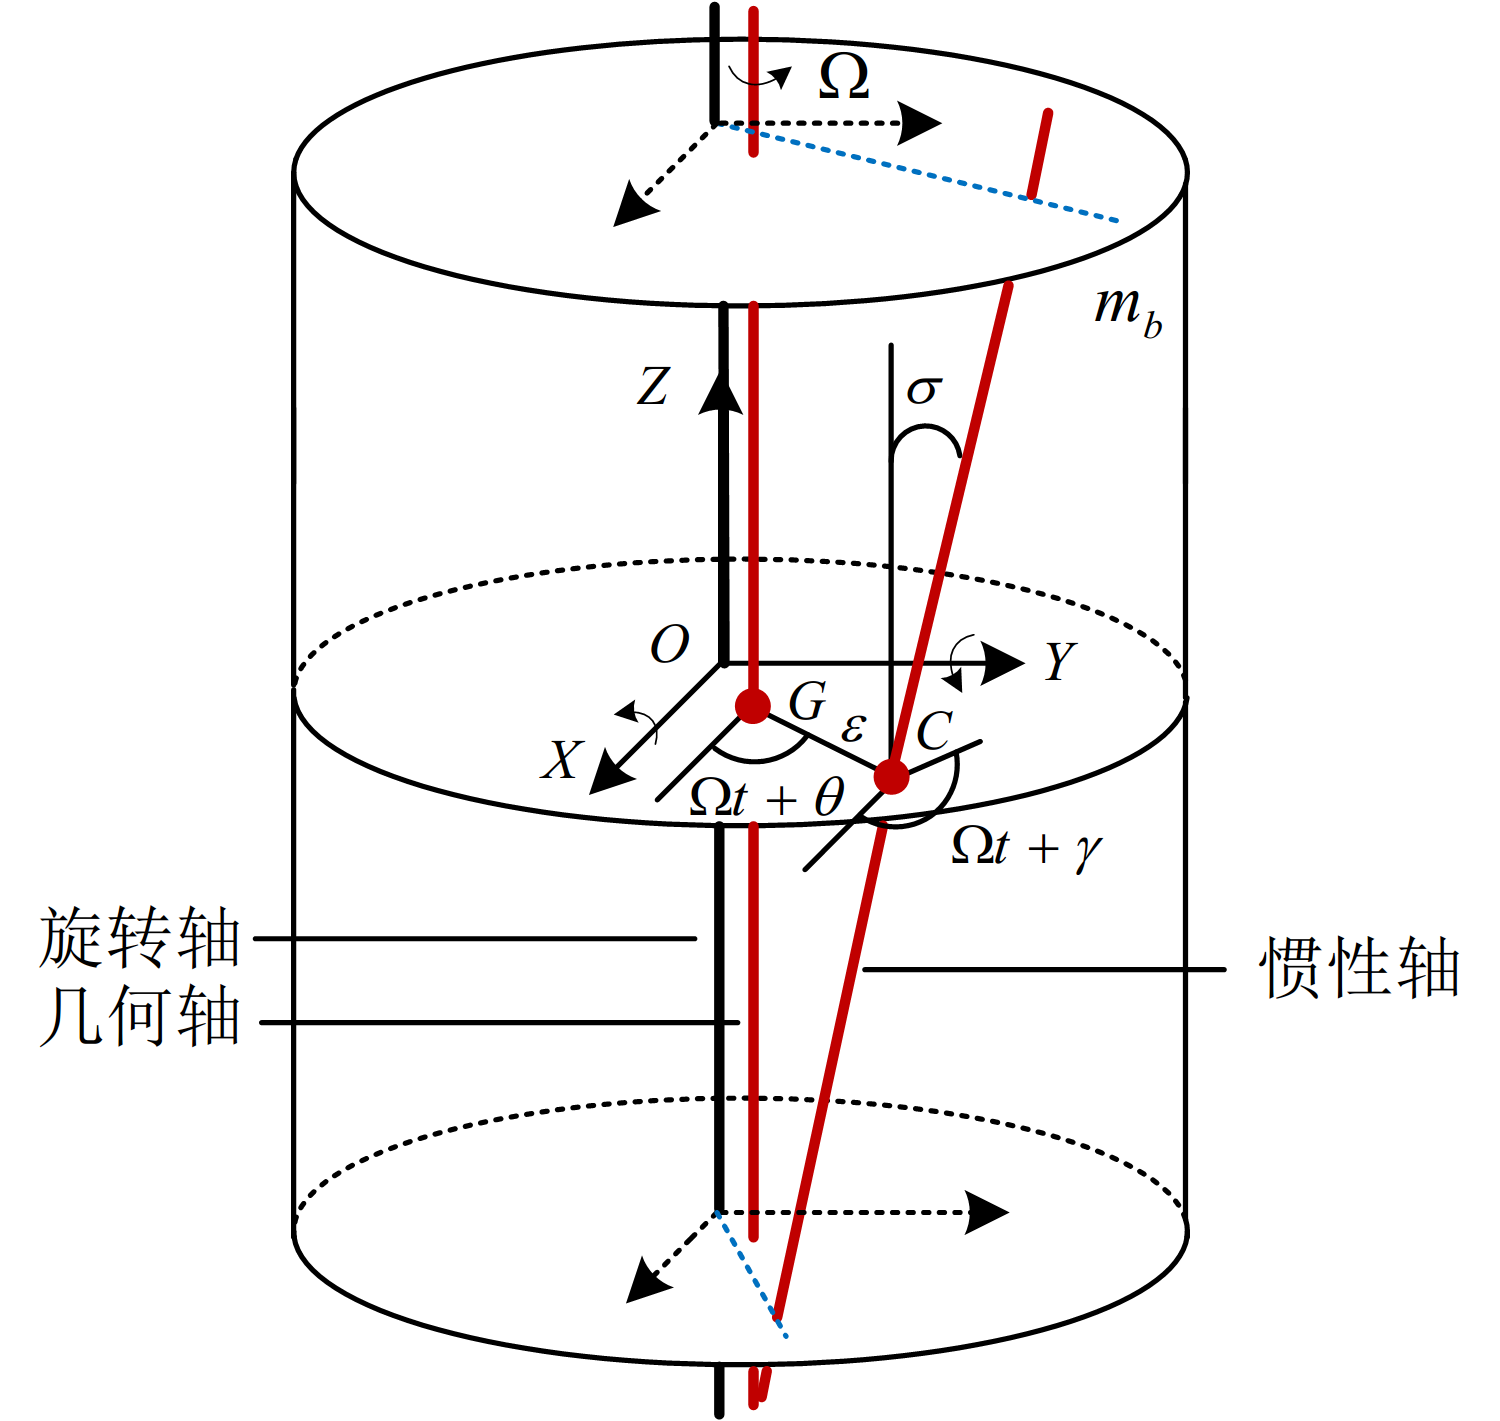
\includegraphics[scale=1.0]{2-2-unbalance.png}
	\caption{转子质量不平衡造成几何轴和惯性轴偏离旋转轴}
	\label{fig:2-2-unbalance}
\end{figure}

转子的不平衡质量造成其几何轴、惯性轴和旋转轴不重合,即质量中心(亦即惯性轴中心)$ q_i $和几何中心(亦即几何轴中心)$ q_g $发生偏离。不平衡质量造成转子静不平衡和动不平衡:静不平衡指几何轴与惯性轴在同一平面上的偏移,在转子旋转时产生振动力;动不平衡是指几何轴和惯性轴因角度偏移而异面,在转子旋转时产生振动力矩,如\autoref{fig:2-2-unbalance}所示。若记该偏移距离为$ q_{\Delta} $,则可以表示
\begin{equation}
\label{eq:q_delta}
{{q}_\Delta }{ = }\left[ 
{\begin{matrix}
   {\sigma \cos \left( {\Omega t + \gamma } \right)}  \cr 
   {e\cos \left( {\Omega t + \theta } \right)}  \cr 
   {\sigma sin\left( {\Omega t + \gamma } \right)}  \cr 
   {e\sin \left( {\Omega t + \theta } \right)}  \cr 
\end{matrix}} 
 \right]
\end{equation}
其中$\sigma$表示动平衡的幅值,$\gamma$表示动不平衡的初相位;$e$表示静平衡的幅值,$\theta$表示静不平衡的初相位。

则几何中心与质量中心的空间关系可以表示为
\begin{equation}
{{q}_i}{ = }{{q}_{g}} + {{q}_\Delta }
\end{equation}

\subsection{位移传感器误差}
\begin{figure}
	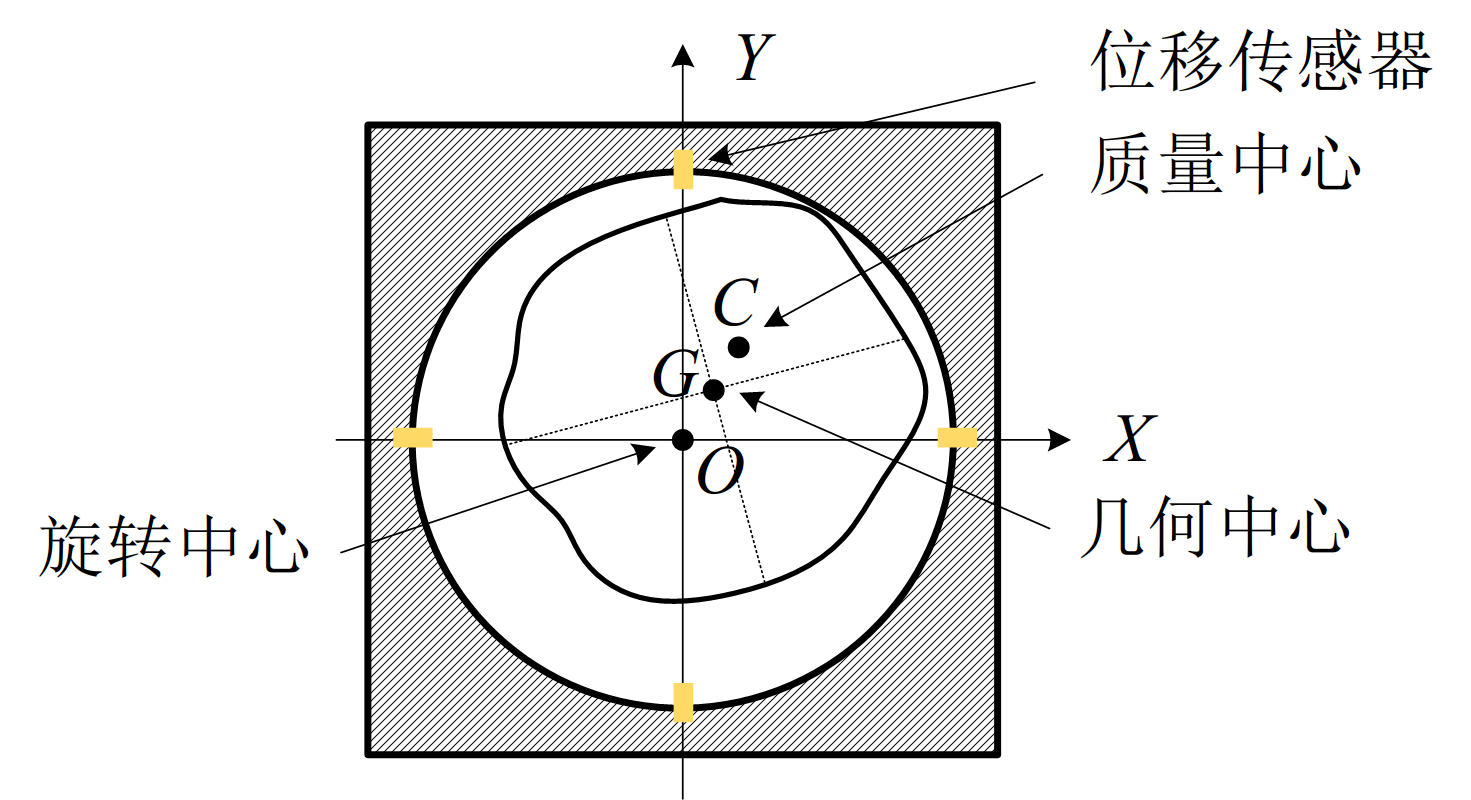
\includegraphics[scale=1.0]{2-3-sensor.png}
	\caption{传感器检测面不均与引起检测误差}
	\label{fig:2-3-sensor}
\end{figure}
三自由度轴向径向磁轴承中,正交方向上的两个自由度的控制分别使用一对位移传感器来检测转子在该磁轴承处的位移。如\autoref{fig:2-3-sensor}所示。由于实际加工精度限制,转子的位移检测面通常不是一个正规、平滑的圆面,而是存在凹凸面的不规则面。由此使转子的测量位移信号中包含多种频率的噪声扰动,导致实际位置无法测得。记扰动信号为
\begin{equation}
\Theta {{q}_s} = \sum\limits_{k = 1}^n {{A_k}\sin \left( {k\Omega t + {\phi _k}} \right)} 
\end{equation}
其中$k$是谐波次数,$A_k$是第$k$次谐波的幅值,$\phi _k$是第$k$次谐波的初相位。记传感器观测的转子位置为${\hat q}_s$,真实的转子位置为$q_s$,则
\begin{equation}
{{\hat q}_s} = {{q}_s} - \Theta {{q}_s}
\end{equation}

\begin{figure}
	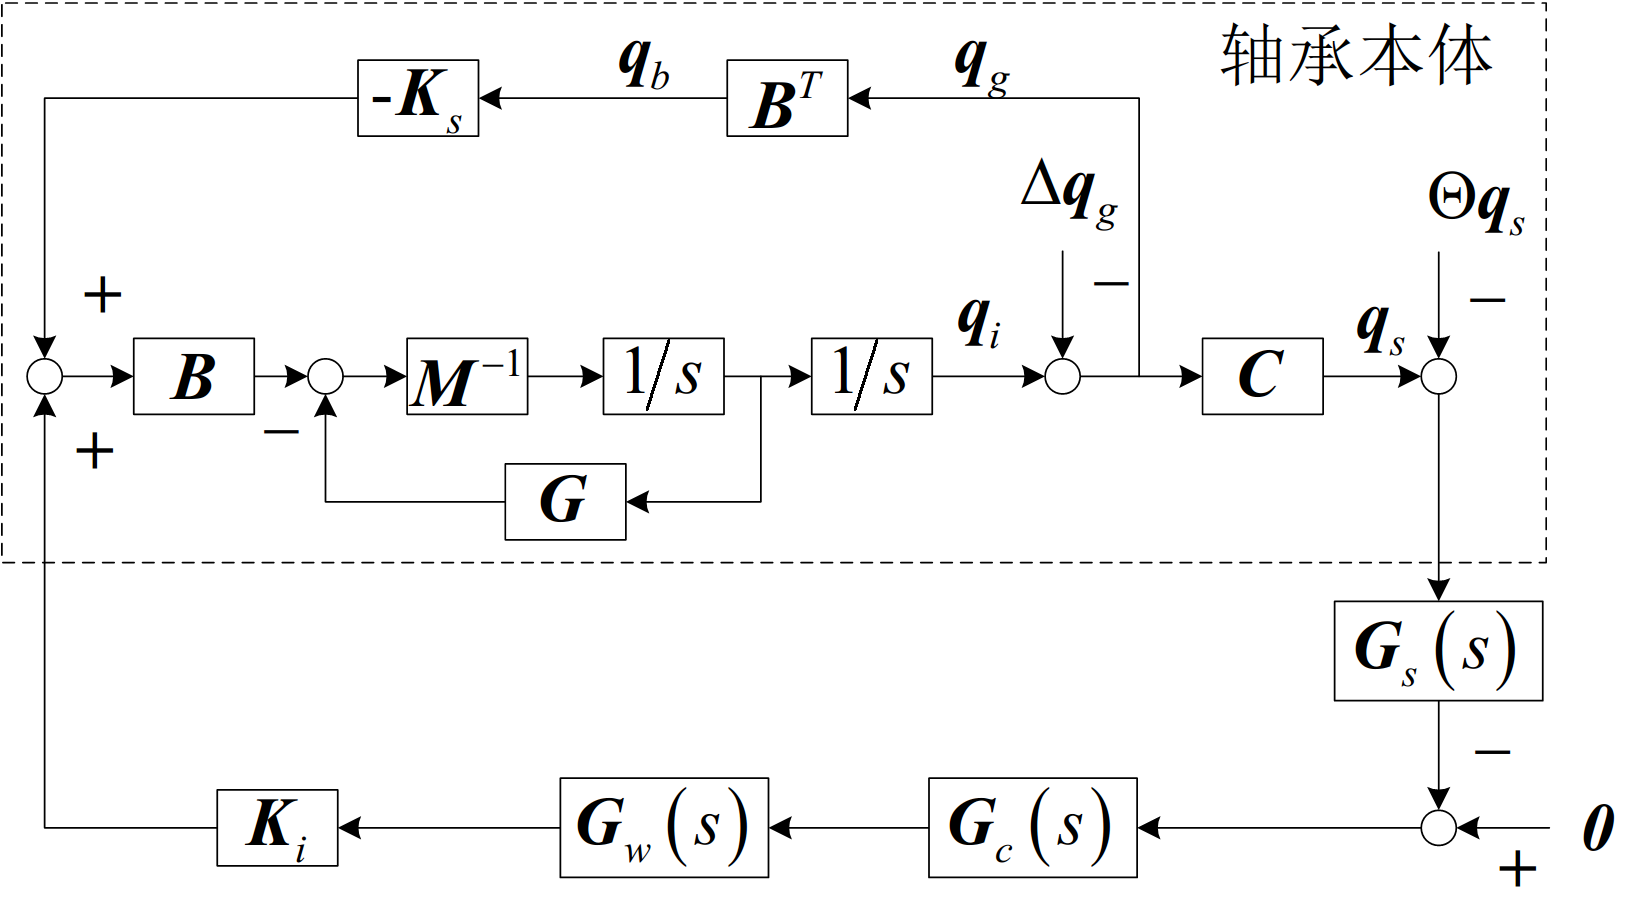
\includegraphics[scale=1.0]{2-4-control.png}
	\caption{磁悬浮轴承系统控制框图}
	\label{fig:2-4-control}
\end{figure}
由于磁轴承和转子组成的系统是一个开环不稳定的控制系统,需要引入闭环控制才能使其保持稳定。其闭环控制框图如\autoref{fig:2-4-control}所示。$G_s(s)$是位移传感器的传递函数,$G_c(s)$是PID控制器的传递函数,$G_w(s)$是功率放大器的传递函数。本文采用分散的PID控制策略,即两端三自由度的轴向径向磁轴承分别控制转子在两端的水平和竖直方向的运动,径向共四个控制通道:$XA$、$YA$、$XB$和$YB$。$G_s(s)$、$G_c(s)$和$G_w(s)$均为$4*4$对角矩阵:
$${G_w}\left( s \right) = \left[ 
{\begin{matrix}
   {{1 \over {s{f_s} + 1}}} & 0 & 0 & 0  \cr 
   0 & {{1 \over {s{f_s} + 1}}} & 0 & 0  \cr 
   0 & 0 & {{1 \over {s{f_s} + 1}}} & 0  \cr 
   0 & 0 & 0 & {{1 \over {s{f_s} + 1}}}  \cr 

 \end{matrix} }
\right]$$

$${G_s}\left( s \right) = \left[ 
{\begin{matrix}
   {{k_{se}}} & 0 & 0 & 0  \cr 
   0 & {{k_{se}}} & 0 & 0  \cr 
   0 & 0 & {{k_{se}}} & 0  \cr 
   0 & 0 & 0 & {{k_{se}}}  \cr 

 \end{matrix} } 
 \right]$$
 
$${G_c}\left( s \right) = \left[ {\begin{matrix}
   {{k_p} + {{{k_i}} \over s} + {k_d}s} & 0 & 0 & 0  \cr 
   0 & {{k_p} + {{{k_i}} \over s} + {k_d}s} & 0 & 0  \cr 
   0 & 0 & {{k_p} + {{{k_i}} \over s} + {k_d}s} & 0  \cr 
   0 & 0 & 0 & {{k_p} + {{{k_i}} \over s} + {k_d}s}  \cr 

 \end{matrix} } \right]$$
考虑质量不平衡和传感器扰动,闭环系统控制方程为

待补充:位移扰动与PID控制器、控制电流的关系;矩阵方程与单自由度控制的关系;为何轴向和径向视为解耦;考虑扰动时的闭环系统控制方程

\section{本章小结}
本节以磁悬浮离心压缩机为例,介绍了磁悬浮电机的机械结构及其控制系统组成。建立了磁悬浮轴承转子的动力学模型,以及包含质量不平衡和传感器误差因素的磁悬浮转子振动模型。本章结论如下:
\begin{enumerate}
\item 五自由度磁悬浮轴承转子的主动控制包含轴向平动、径向平动和转动,其中轴向运动和径向运动可视为解耦控制。
\item 质量不平衡可视为在传感器检测点引入的与转子转速同频的正弦扰动,此正弦扰动会在控制电流中引起与之同频正弦扰动电流,进而在磁轴承中产生与之同频的正弦扰动磁悬浮力。
\item 传感器误差在传感器检测点引入与转子转速成一倍或多倍关系的正弦扰动,与质量不平衡类似,最终在控制电流和磁轴承中激发谐波成分丰富的扰动成分。
\end{enumerate}
\chapter{基于重复控制器的主动振动控制方法}
本章分析了重复控制器的原理,包括基本成分、稳定性分析和应用拓扑。针对磁悬浮轴承中的同频和倍频正弦扰动,提出了一种新的重复控制器算法——零相移奇数次重复控制器,解决了传统重复控制器相位延迟问题,同时提升了算法收敛速度。仿真结果表明零相移奇数次重复控制器可以有效抑制控制电流中的同频以及倍频扰动。
\section{传统整数次重复控制器}
\subsection{工作原理}
重复控制器是基于内模原理\cite{francis1975internal},其证明了在存在扰动信号的条件下,欲使闭环系统无误差地跟踪给定输入指令,一个充分条件是闭环系统中包含这个扰动信号模型。例如,在离散域下一个周期为$N$的信号可以表示为
\begin{equation}
\label{eq3-1}
W\left( z \right){\rm{ = }}{{{W_0}} \over {1 - {z^{ - N}}}}
\end{equation}

\begin{figure}
	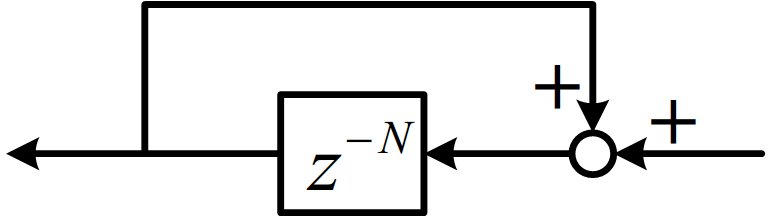
\includegraphics[scale=1.0]{3-1-generator.png}
	\caption{一种周期信号发生器}
	\label{fig:3-1-generator}
\end{figure}

其中${W_0}\left( z \right) = w\left( 0 \right) + w\left( 1 \right){z^{ - 1}} + ... + w\left( {N - 1} \right){z^{ - \left( {N - 1} \right)}}$。针对该周期信号,可以构造其对应的信号模型如\autoref{fig:3-1-generator}所示。该环节的离散域传递函数为
\begin{equation}
\label{eq3-2}
{G_{rc}}\left( z \right){\rm{ = }}{{{z^{ - N}}} \over {1 - {z^{ - N}}}}
\end{equation}
其中$N = {{{\omega _s}} \mathord{\left/
 {\vphantom {{{\omega _s}} {{\omega _d}}}} \right.
 \kern-\nulldelimiterspace} {{\omega _d}}}$,$\omega _s$是数字控制器的采样角频率,$\omega _d$是扰动信号的基波角频率。可以看出,$G_{rc}(z)$的极点在$\omega = k\omega_d(k = 1,2,...)$处,因此对于频率为整数倍于基波频率的信号,包含该周期信号发生器的闭环回路均具有消除扰动信号、无误差跟踪给定输入指令的能力。
 
\begin{figure}
	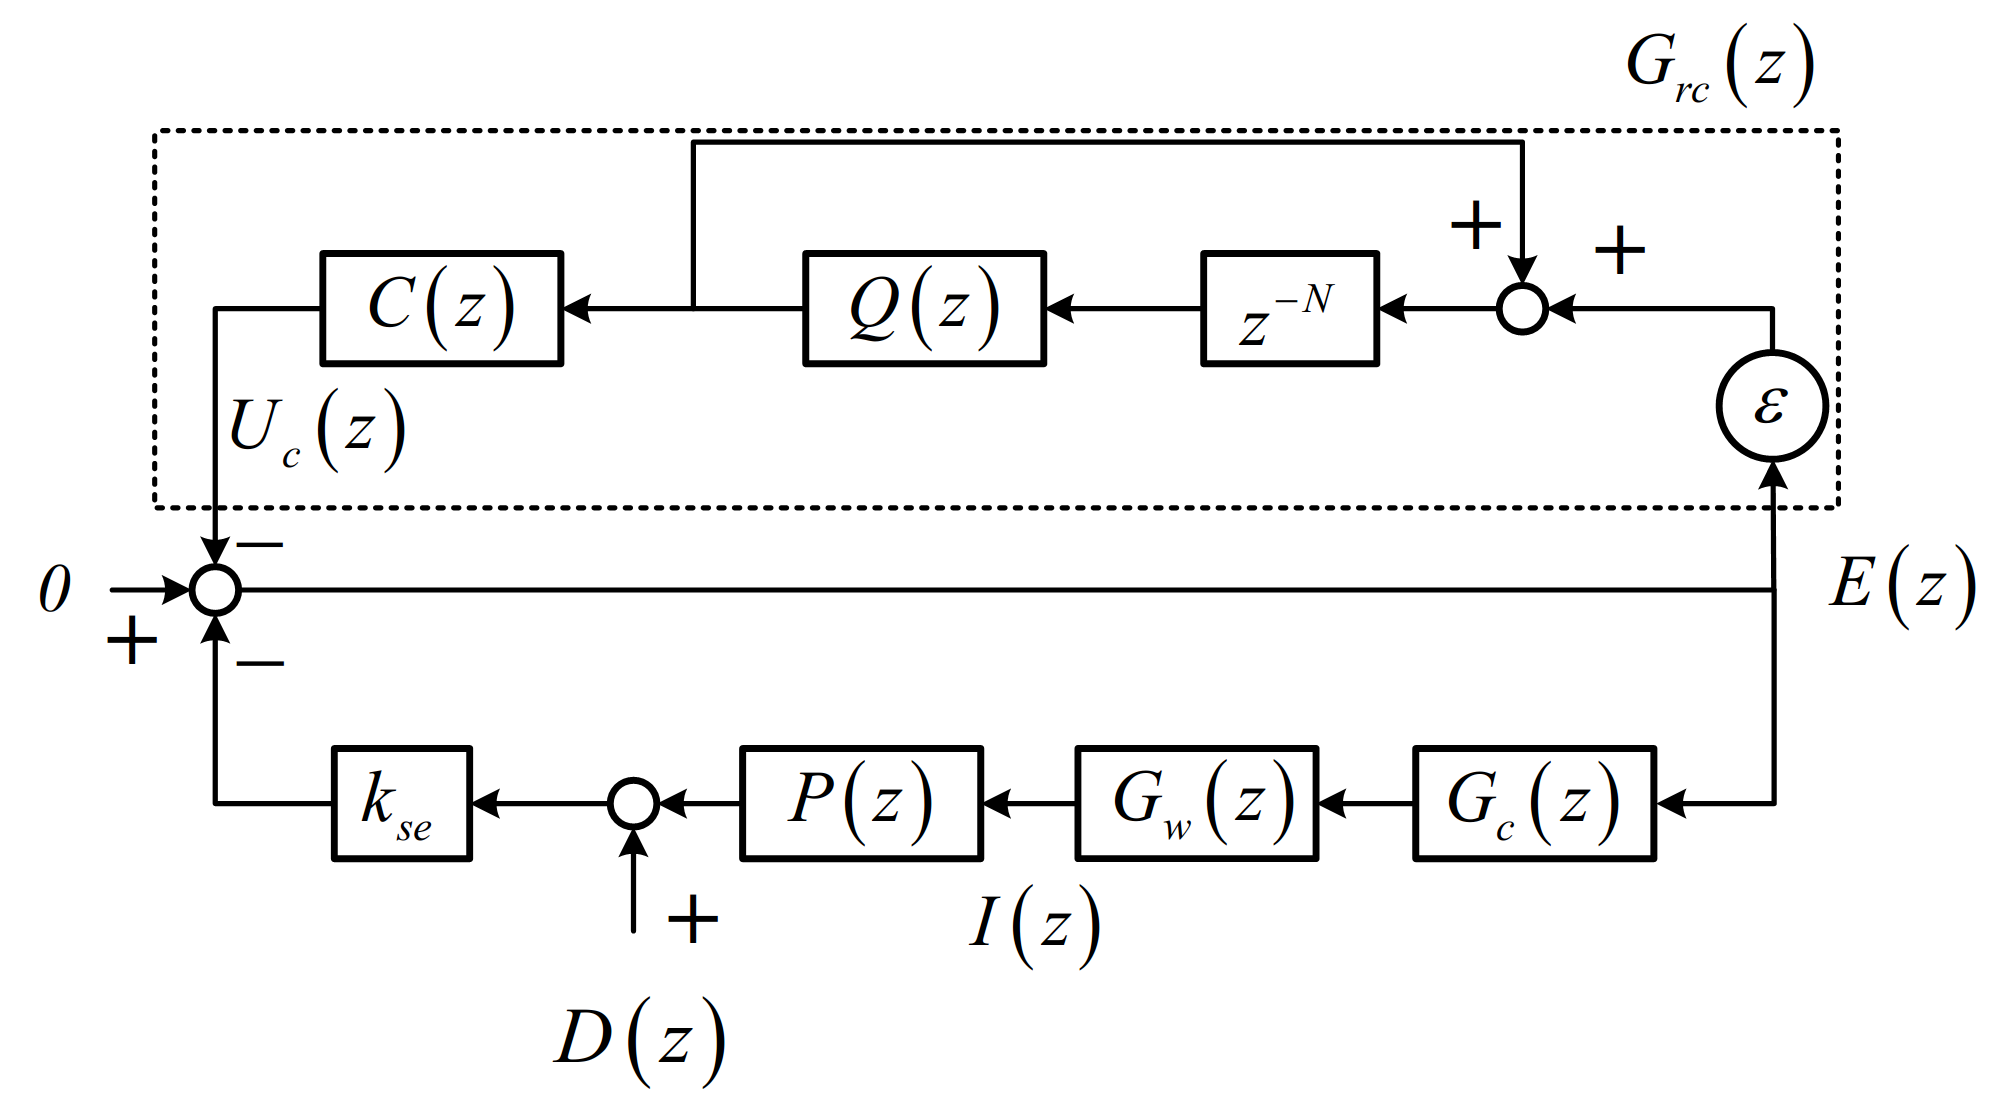
\includegraphics[scale=1.0]{3-2-crc.png}
	\caption{使用重复控制器抑制电流谐波的控制框图}
	\label{fig:3-2-crc}
\end{figure}

磁悬浮轴承位移传感器中的同频和倍频扰动信号造成控制电流中包含谐波含量丰富的振动信号,为消除振动电流以抑制振动力,通常以反馈形式插入重复控制器,应用拓扑如\autoref{fig:3-2-crc}所示。虚线框所围区域是插入的重复控制器,其由以下部分构成:
\begin{enumerate}
	\item 控制增益$\varepsilon $:用于调节插入式重复控制器的作用强度,该值越大,重复控制器作用强度越强,即谐波扰动信号抑制越明显。但是随着控制增益的增大,闭环回路的稳定性在随之下降。
	\item 延时环节${z^{ - N}}$:用于记忆前某段时刻至当前时刻的波形,延时环节的个数与扰动信号频率、控制频率相关。
	\item 低通滤波器$Q(z)$:由于实际需要被消除的周期信号中同时含有噪声等无效信号,经过延时环节的累计记忆后可能导致环路输出发散,闭环回路失稳。因此加入低通滤波器来抑制高频噪声,提升重复控制器稳定范围。
	\item 相位补偿器$C(z)$:控制信号输入到重复控制器回路后,经过延时环节和低通滤波器环节后存在幅值和相位的变化,相位调节器用于调节重复控制器回路的相位,提升重复控制器的稳定范围。
\end{enumerate}

位移传感器和质量不平衡引起的同频或者倍频扰动信号可以等效为位移传感器前级引入的扰动信号,将该外源扰动记为$D(z)$。将磁轴承线圈电流信号记为$I(z)$,谐波抑制的目的是使$I(z)$中谐波成分降低。

该插入式重复控制器的输入为位移误差信号$E(z)$,记重复控制器的输出为$U_c(z)$,那么重复控制器的计算规律可以表示为
\begin{equation}
{U_c}\left( z \right) = \frac{{\varepsilon  \cdot {z^{ - N}}Q\left( z \right)C\left( z \right)E\left( z \right)}}{{1 - {z^{ - N}}Q\left( z \right)}}
\label{eq3-3}
\end{equation}
重复控制器的开环传递函数记为$G_{rc}(z)$,其可以表示为
\begin{equation}
{G_{rc}}\left( z \right) = \frac{{{U_c}\left( z \right)}}{{E\left( z \right)}} = \frac{{{z^{ - N}}Q\left( z \right)}}{{1 - {z^{ - N}}Q\left( z \right)}}\varepsilon C\left( z \right)
\label{eq3-4}
\end{equation}
扰动信号$D(z)$到电流信号$I(z)$的传递函数记为$L_1(z)$,其可以表示为
\begin{equation}
{L_1}\left( z \right) = {L_0}\left( z \right) \cdot \frac{{1 - {z^{ - N}}Q\left( z \right)}}{{1 - {z^{ - N}}Q\left( z \right)\left[ {1 - \varepsilon \frac{{C\left( z \right){L_0}\left( z \right)}}{{{k_{se}}{G_c}\left( z \right){G_w}\left( s \right)}}} \right]}}
\label{eq3-5}
\end{equation}
其中
\begin{equation}
{L_0}\left( z \right) =  - \frac{{{k_{se}}{G_w}\left( z \right){G_c}\left( z \right)}}{{1 + {k_{se}}{G_c}\left( z \right)P\left( z \right)}}
\label{eq3-6}
\end{equation}
假设传递函数的极点在单位圆内,即闭环系统是稳定的(详细稳定性分析过程见下节)。记低通滤波器的截止频率为$\omega_c $,在$\omega<\omega_c$内,近似存在$Q(z)=1$。那么控制目标$I(z)$在与扰动信号基波频率成整数倍的频率处存在若干零点,即
\begin{equation}
\label{eq3-7}
\mathop {\lim }\limits_{\omega  \to {\omega _e}} \left\| {I\left( {j\omega } \right)} \right\| = 0
\end{equation}
其中 $\omega _e=\omega _0, 2\omega _0,...,n\omega _0$ ($n\omega _0$$<$$\omega _c$, $\omega _0$是扰动信号基波频率)。磁轴承中,扰动信号基波频率即转子旋转频率。\autoref{eq3-7}说明:插入重复控制器且闭环系统保持稳定的情况下,线圈电流中的与转子同频以及倍频扰动信号可以被消除。
\subsection{稳定性分析}
磁悬浮轴承系统灵敏度函数是表征磁轴承闭环系统控制性能的一个重要特征,它是指给定位移信号到位移误差信号的传递函数,可以用来衡量闭环系统的稳定性。系统灵敏度函数的峰值越低,系统的稳定性能越好。\autoref{fig:3-2-crc}所示的插入重复控制器的闭环系统中,加入插入式重复控制器前,系统灵敏度函数记为$S_0(s)$,其可以表示为
\begin{equation}
{S_0}\left( z \right) = {{E\left( z \right)} \over {D\left( z \right)}}{\rm{ = }}{1 \over {1 + {G_c}\left( z \right)P\left( z \right){G_s}\left( z \right)}}
\end{equation}
扰动信号$D(z)$到电流信号$I(z)$的传递函数记为$L_0(z)$,其可以表示为
\begin{equation}
{L_0}\left( z \right) = {{I\left( z \right)} \over {D\left( z \right)}}{\rm{ = }} - {{{G_c}\left( z \right){G_s}\left( z \right)} \over {1 + {G_c}\left( z \right)P\left( z \right){G_s}\left( z \right)}}
\end{equation}
加入插入式重复控制器后,扰动信号$D(z)$到电流信号$I(z)$的传递函数记为$L_1(z)$,其可以表示为
\begin{equation}
\label{eq3-10}
\begin{aligned}
L_1(z)
&=\dfrac{I(z)}{D(z)}\\
&=\dfrac{G_c(z)G_s(z)}{1+G_c(z)P(z)G_s(z)+\dfrac{z^{-N}Q(z)}{1-z^{-N}Q(z)}\varepsilon C(z)}\\
&=\dfrac{G_c(z)G_w(z)}{1+G_c(z)P(z)G_s(z)}\cdot \dfrac{1}{1+\dfrac{z^{-N}Q(z)}{[1-z^{-N}Q(z)][1+G_c(z)P(z)G_s(z)]}\varepsilon C(z)}\\
&=\dfrac{G_c(z)G_w(z)}{1+G_c(z)P(z)G_s(z)}\cdot \dfrac{1-z^{-N}Q(z)}{1-z^{-N}Q(z)\left[1-\dfrac{1}{1+G_c(z)P(z)G_s(z)}\varepsilon C(z)\right]}\\
&=L_0(z)\dfrac{1-z^{-N}Q(z)}{1-z^{-N}Q(z)[1-\varepsilon C(z)S_0(z)]}
\end{aligned}
\end{equation}
闭环系统的稳定性充分必要条件是其在$s$域右半平面没有极点,等效于在$z$域上极点均在单位圆内。从\autoref{eq3-10}可以看出,加入插入式重复控制器的闭环系统稳定条件是:
\begin{enumerate}
	\item 系统灵敏度函数$S_0(z)$的极点在单位圆内;
	\item $\left\| Q(z)[1 - \varepsilon C(z)S_0(z)] \right\| < 1$
\end{enumerate}
通常在加入插入式重复控制器之前,通过设计合适的控制器$G_c(z)$的参数来使闭环系统稳定。因此条件1通常在加入插入式重复控制器之前得到满足。通过设计合适的重复控制器参数,包括$\varepsilon$、$Q(z)$、$C(z)$来使加入插入式重复控制器的系统保持稳定。
\section{奇数次零相移重复控制器}
磁悬浮轴承中谐波扰动信号通常是奇数倍于基波频率,使用传统整数次重复控制器可以消除所有奇数次谐波扰动,但是其在偶数谐波出的抑制作用是冗余的。如果重复控制器可以仅在奇数次频率处起作用,那么加入的插入式重复控制器可以避免对偶数次频率处的系统特性产生影响。

此外,为了维持闭环系统的稳定性,重复控制器环路中的低通滤波器是必不可少的组成成分。然而低通滤波器对有效信号的幅值衰减和相位偏移特性将会导致重复控制器谐波抑制作用减弱。

针对传统整数次重复控制器的在磁轴承中应用的弊端,本节提出一种奇数次零相移低通滤波器,其改进点在于:
\begin{enumerate}
	\item 将整数次重复控制器中的整数次周期信号发生器改为奇数次周期信号发生器,使得重复控制器仅消除奇数次谐波;
	\item 将低通滤波器从重复控制器延时环路内移动到延时环路外,保证闭环系统稳定性的同时,可以有效提高重复控制器谐波抑制能力;
	\item 将传统的一阶低通滤波器改为零相移低通滤波器,保留其对信号幅值衰减特性的能力,同时避免对信号的相位偏移。
\end{enumerate}
\subsection{工作原理}
对于\autoref{eq3-2}所表示的周期信号模型,其可以分解表示为
\begin{equation}
G_{rc}(z)=\dfrac{1}{2}\left(\dfrac{1}{1-z^{-N/2}}-\dfrac{1}{1+z^{-N/2}}\right)
\end{equation}
代入$N=\dfrac{\omega_s}{\omega_D}$、$z=e^{j\omega T_s}$其中$\omega_s$是信号采样角频率,$\omega_D$是扰动信号基波频率,$T_s$是采样周期。那么上式可以表示为
\begin{equation}
G_{rc}(j\omega)=\frac{1}{2}\left(\frac{1}{1-e^{-j\pi\frac{\omega}{\omega_D}}}-\frac{1}{1+e^{-j\pi\frac{\omega}{\omega_D}}}\right)
\end{equation}
对于${1}/\left(1-e^{-j\pi\frac{\omega}{\omega_D}}\right)$,其极点在$\omega=2k\omega_D$处$(k=0,1,2,..)$,该项可以消除频率是偶数倍于基波频率的扰动信号;对于${1}/\left(1+e^{-j\pi\frac{\omega}{\omega_D}}\right)$,其极点在$\omega=(2k-1)\omega_D$处$(k=0,1,2,..)$,该项可以消除频率是奇数倍于基波频率的扰动信号。

若将\autoref{eq3-2}所表示的周期信号模型称之为整数次周期信号发生器,那么由上述推导可见,其可以分解成为奇数次信号发生器和偶数次信号发生器,如\autoref{fig:3-3-odd_generator}所示。仅取其奇数次周期信号发生器部分,替换传统重复控制器中的整数次周期信号发生器部分,即构成奇数次重复控制器。
\begin{figure}
	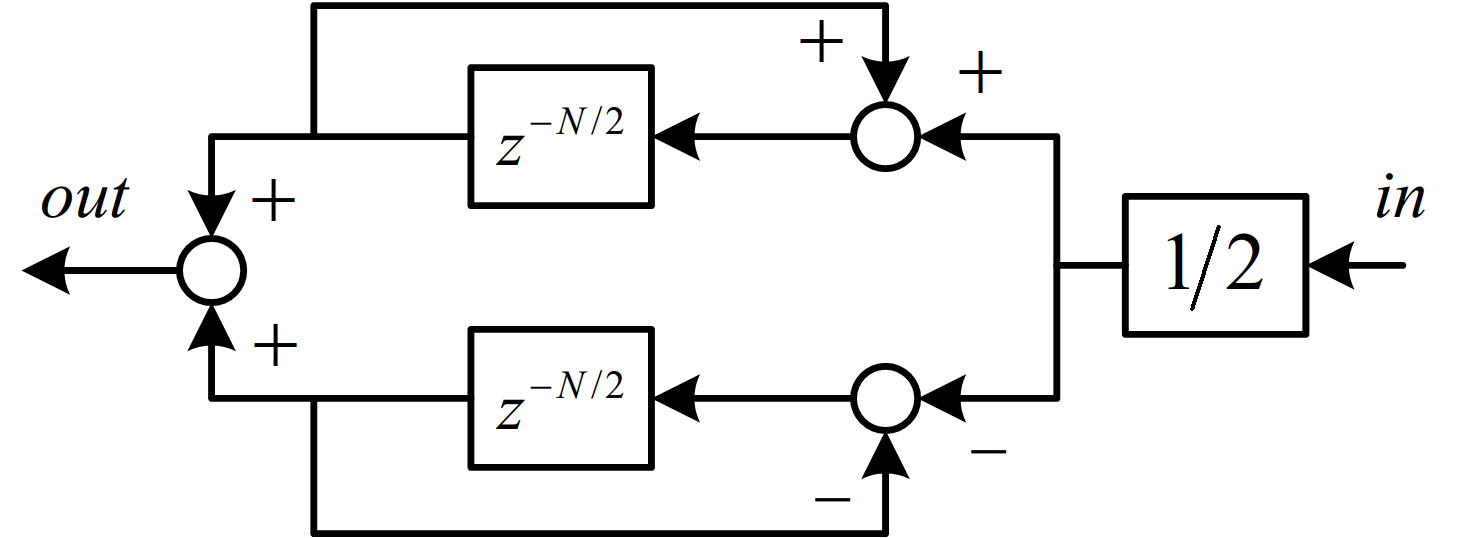
\includegraphics[scale=1.0]{3-3-odd_generator.png}
	\caption{奇数次、偶数次信号发生器组合示意图}
	\label{fig:3-3-odd_generator}
\end{figure}
加入插入式奇数次重复控制器的磁轴承系统控制框图如\autoref{fig:orc}所示。
\begin{figure}
	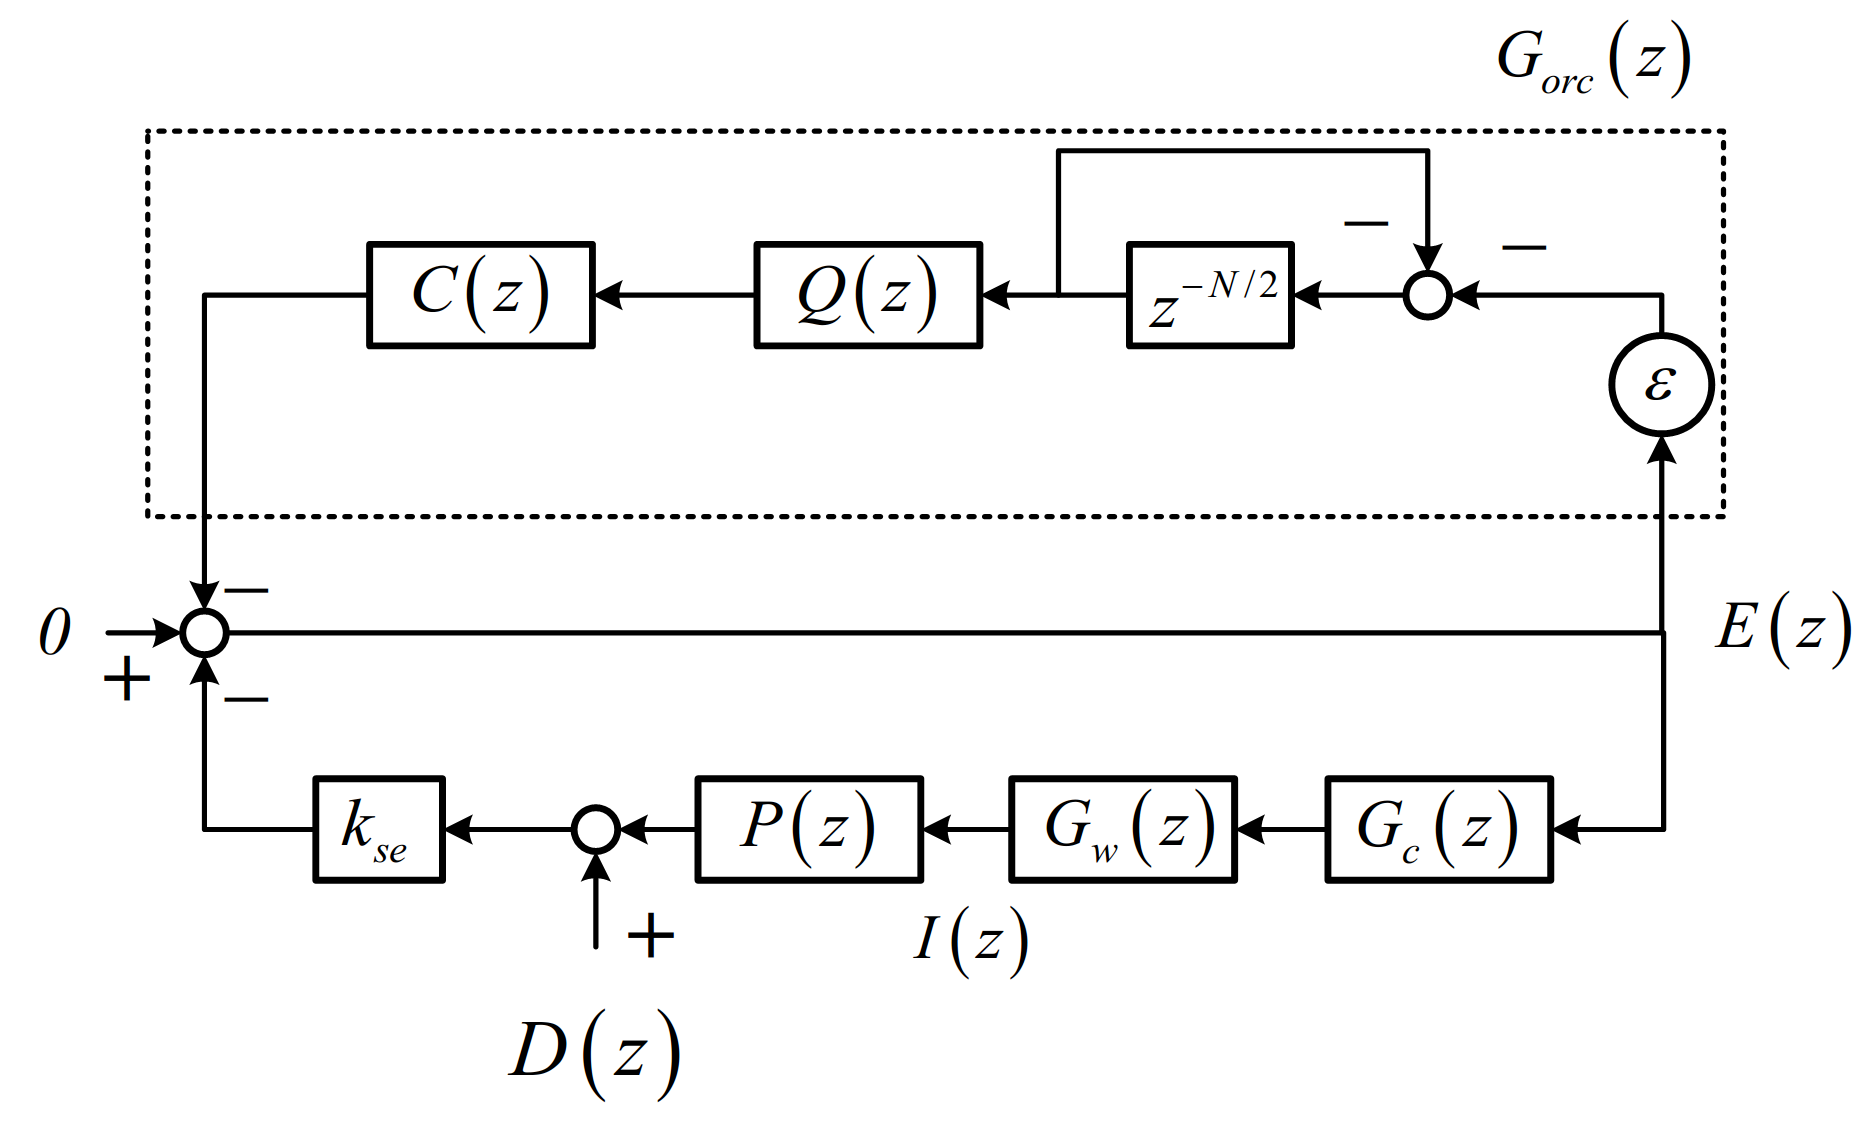
\includegraphics[scale=1.0]{3-4-orc.png}
	\caption{使用奇数次重复控制器抑制电流谐波的控制框图}
	\label{fig:orc}
\end{figure}
奇数次重复控制器的开环传递函数记为$G_{orc}(z)$,其可以表示为
\begin{equation}
G_{orc}(z)=\dfrac{z^{-N}}{1-z^{-N}Q(z)}\varepsilon C(z)
\end{equation}
记扰动信号$D(z)$到控制电流信号$I(z)$的传递函数为$L_2(z)$,其可以表示为
\begin{equation}
L_1(z)={L_0}\left( z \right) \cdot {{1 + {z^{ - N/2}}} \over {1 - {z^{ - N/2}}\left[ {\varepsilon Q\left( z \right)C\left( z \right){S_0}\left( z \right) - 1} \right]}}
\end{equation}
假设传递函数的极点在单位圆内,即闭环系统是稳定的(详细稳定性分析过程见下节)。那么控制目标$I(z)$在与扰动信号基波频率成奇数倍的频率处存在若干零点,即
\begin{equation}
\label{eq3-10_1}
\mathop {\lim }\limits_{\omega  \to {\omega _e}} \left\| {I\left( {j\omega } \right)} \right\| = 0
\end{equation}
其中 $\omega _e=\omega _0, 3\omega _0,...,(2k-1)\omega _0$ ($\omega _0$是扰动信号基波频率)。\autoref{eq3-10_1}说明:插入奇数次重复控制器且闭环系统保持稳定的情况下,线圈电流中的与转子同频以及奇数倍频扰动信号可以被消除。
\subsection{稳定性分析}
加入插入式重复控制器后,扰动信号$D(z)$到电流信号$I(z)$的传递函数记为$L_2(z)$,其可以表示为
\begin{equation}
\label{eq3-11}
\begin{aligned}
L_2(z)
&=\dfrac{I(z)}{D(z)}\\
&=\dfrac{G_c(z)G_s(z)}{1+G_c(z)P(z)G_s(z)+\dfrac{z^{-N}}{1-z^{-N}Q(z)}\varepsilon C(z)}\\
&=\dfrac{G_c(z)G_w(z)}{1+G_c(z)P(z)G_s(z)}\cdot \dfrac{1}{1+\dfrac{z^{-N}}{[1-z^{-N}Q(z)][1+G_c(z)P(z)G_s(z)]}\varepsilon C(z)}\\
&=\dfrac{G_c(z)G_w(z)}{1+G_c(z)P(z)G_s(z)}\cdot \dfrac{1-z^{-N}}{1-z^{-N}Q(z)\left[1-\dfrac{1}{1+G_c(z)P(z)G_s(z)}\varepsilon C(z)\right]}\\
&=L_0(z)\dfrac{1-z^{-N}}{1-z^{-N}Q(z)[1-\varepsilon C(z)S_0(z)]}
\end{aligned}
\end{equation}
闭环系统的稳定性充分必要条件是其在$s$域右半平面没有极点,等效于在$z$域上极点均在单位圆内。从\autoref{eq3-11}可以看出,加入插入式重复控制器的闭环系统稳定条件是:
\begin{enumerate}
	\item 系统灵敏度函数$S_0(z)$的极点在单位圆内;
	\item 
	\begin{equation}
		\label{eq_stable_odd}
		\left\|1 - \varepsilon C(z)S_0(z) \right\| < 1
	\end{equation}
\end{enumerate}
与应用传统插入式整数次重复控制器类似,通常在加入插入式重复控制器之前,通过设计合适的控制器$G_c(z)$的参数来使闭环系统稳定。因此条件1通常在加入插入式重复控制器之前得到满足。通过设计合适的重复控制器参数,包括$\varepsilon$、$Q(z)$、$C(z)$来使加入插入式奇数次零相移重复控制器的系统保持稳定。
\subsection{零相移低通滤波器设计}
在设计参数控制增益$\varepsilon$和相位调节器$C(z)$之前,需要分析低通滤波器$Q(z)$的参数特性。低通滤波器用于提升重复控制器的稳定范围,理想的低通滤波器是在截止频率前的增益衰减比例为1,截止频率之后频率-增益曲线下降斜率大。传统整数次重复控制器中采用一阶低通滤波器,其形式为:
\begin{equation}
Q(s)=\dfrac{1}{\dfrac{s}{2\pi\cdot f_c}+1}
\end{equation}
该形式的低通滤波器具有形式简单、阶数低的优点,但是其截止频率处的下降斜率并不足够大。此外,该低通滤波器将引入相位延迟,降低重复控制器的抑制能力。为克服以上弊端,一种更优的低通滤波器是零相移低通滤波器。

零相移低通滤波器是一种非因果滤波器,其当前时刻的输出取决于当前时刻的输入和下一时刻的输入。在常规的线性系统中,非因果滤波器无法实现,因为滤波器无法预知下一时刻的输入信号;而在重复控制器环路中,由于若干延时单元的存在,对于其中的非因果滤波器来说,其下一时刻的输入是预先知道的。因此在重复控制器中,非因果滤波器是可以实现的。

本文采用的非因果低通滤波器形式如下
\begin{equation}
\label{eq3-18}
Q(z)=az+b+az^{-1}
\end{equation}
其中$a$和$b$是待设计的滤波器参数。用角频率表示\autoref{eq3-18}:
\begin{equation}
\label{eq3-19}
Q(j\omega)=ae^{j\omega T_s}+b+ae^{-j\omega T_s}
\end{equation}
对\autoref{eq3-19}使用欧拉公式得到:
\begin{equation}
\label{eq3-20}
Q(j\omega)=2a\cdot cos(\omega T_s)+b
\end{equation}
从\autoref{eq3-20}可以看出$Q(j\omega)$没有虚部,因此在重复控制器环路中,该低通滤波器不会引入相位偏移。为了在低通滤波器截止频率前得到单调下降的的幅频曲线,参数$a$和$b$需要满足以下条件:
\begin{equation}
\label{eq3-21}
2a<b
\end{equation}
为了寻找一组较优的$Q(z)$参数,研究不同参数下的幅频曲线。以工作转速为250Hz为例,此工况下系统中的主要谐波成分为250Hz、750hz、1250Hz和1750Hz,欲消除七次及以下谐波,则低通滤波器的截止频率应该略高于1750Hz,此处取2250Hz。
\begin{figure}
	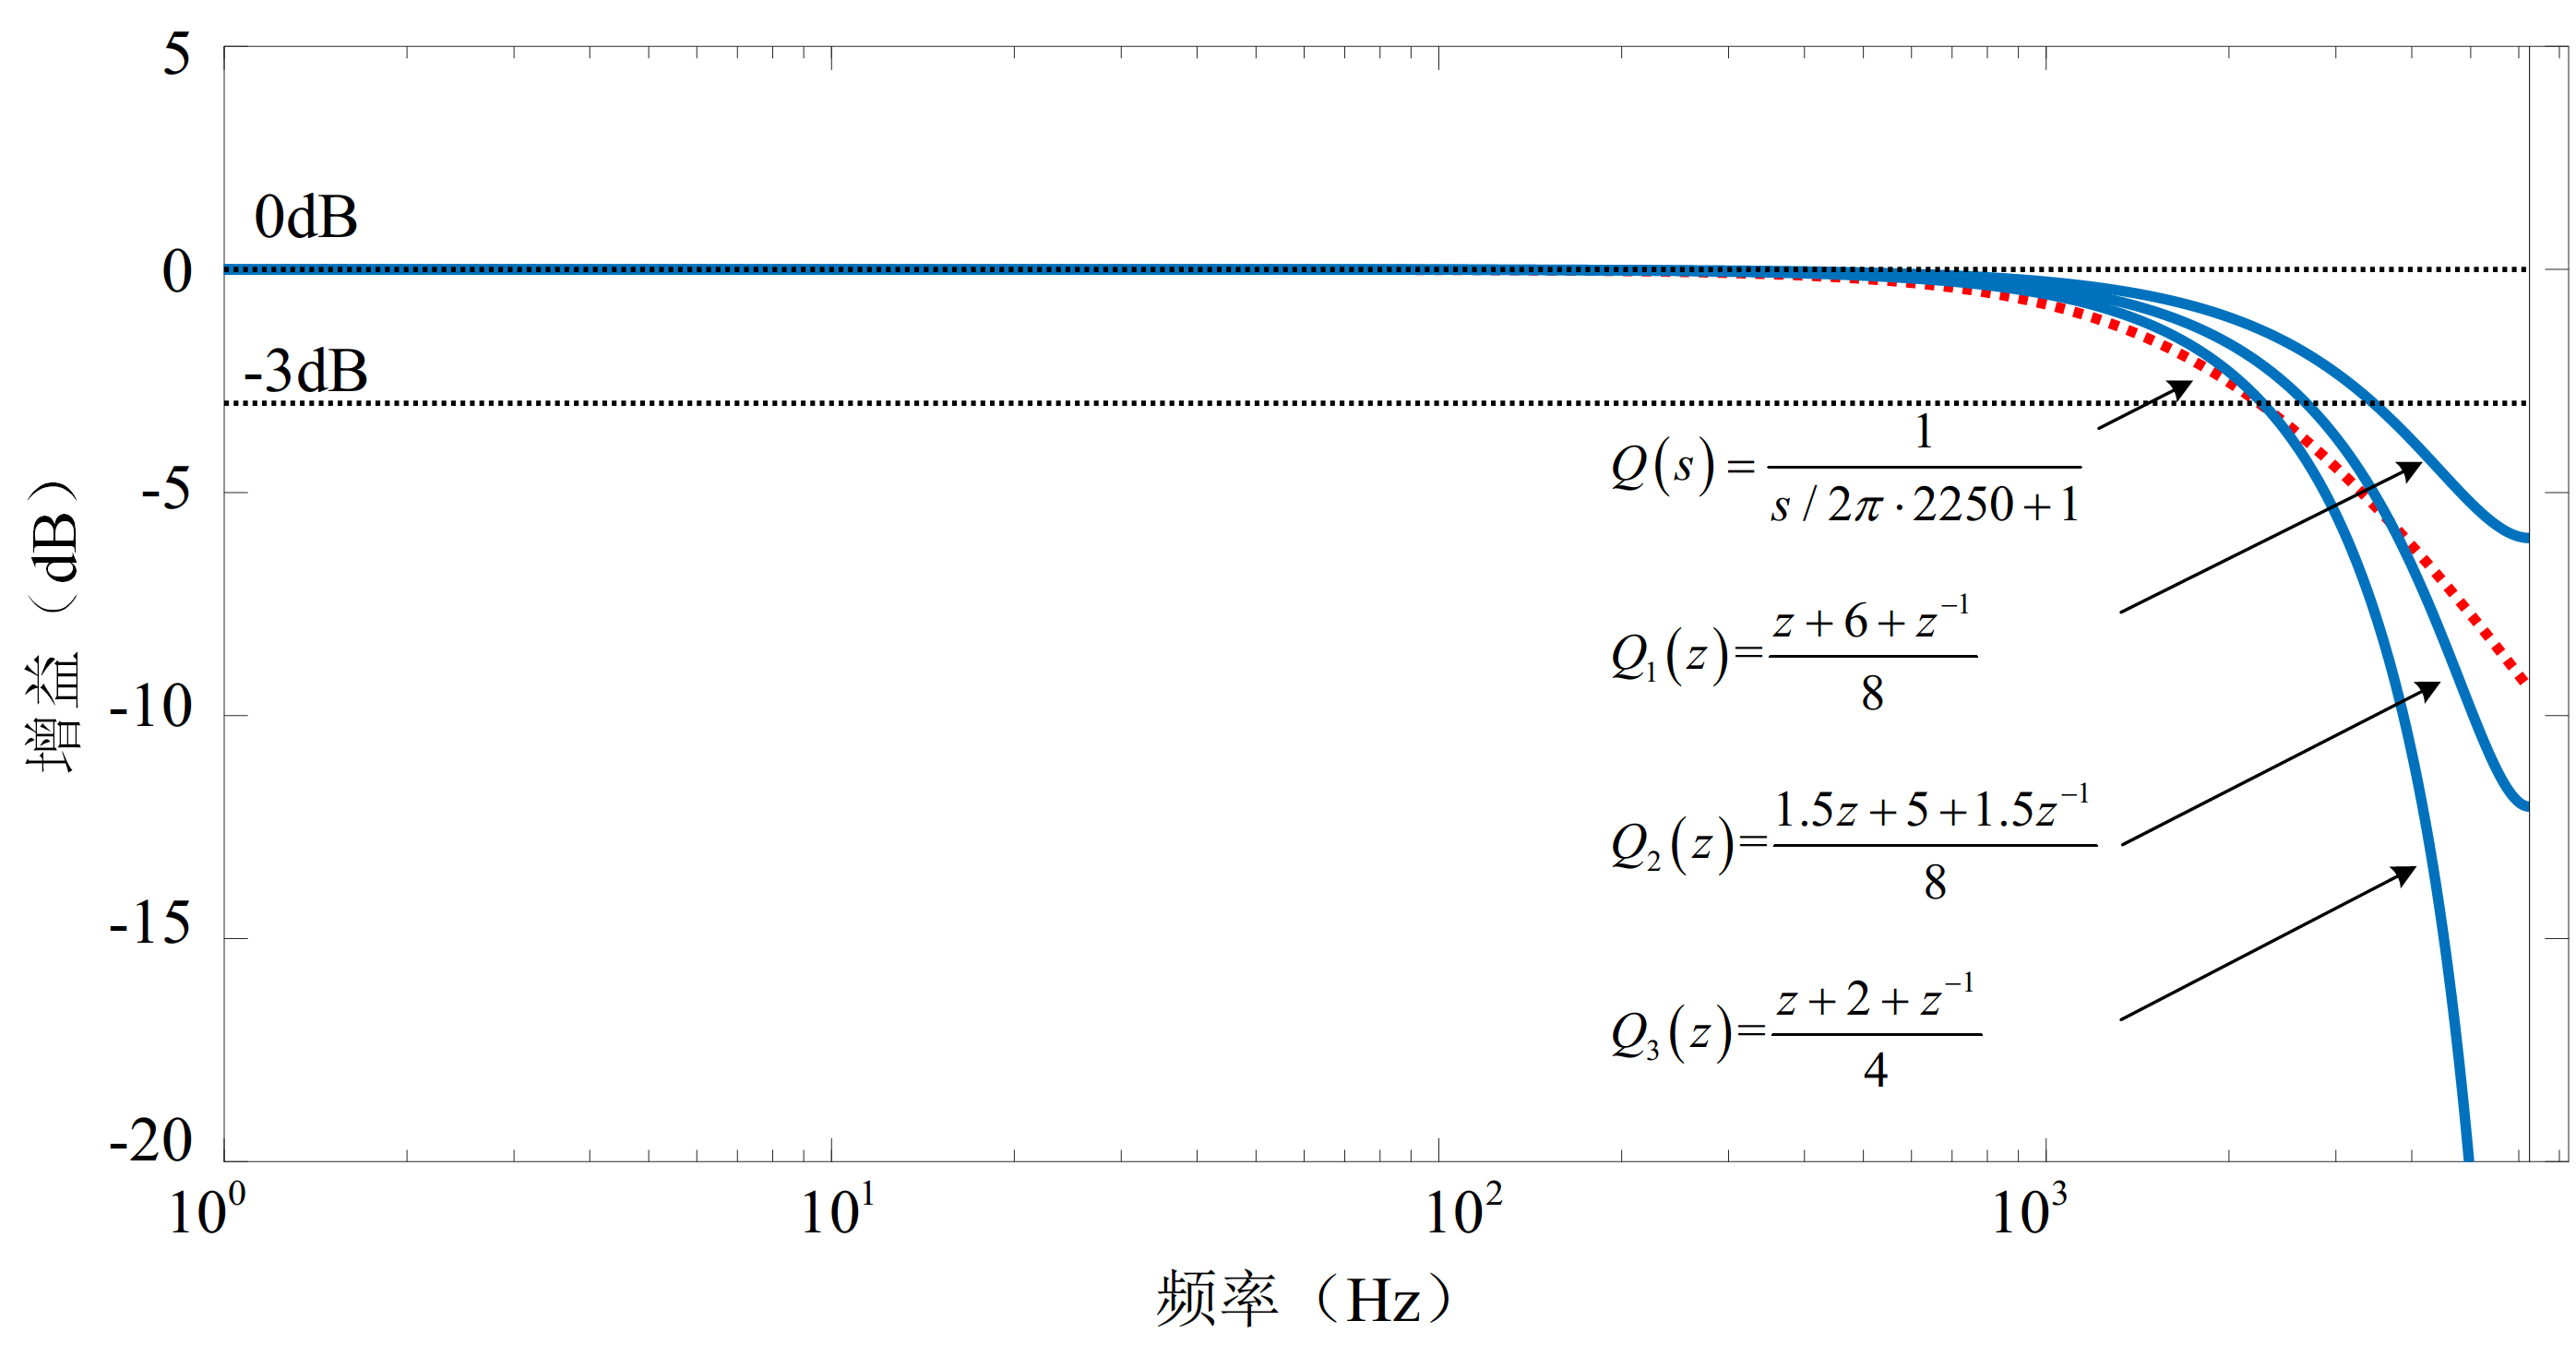
\includegraphics[scale=1.0]{3-5-lpf.png}
	\caption{不同参数下的低通滤波器幅频曲线}
	\label{fig:3-5-lpf}
\end{figure}

从\autoref{fig:3-5-lpf}可见,与一阶低通滤波器$Q(s)$相比,$Q_3(z)$在低频处的增益更接近0dB,同时在截止频率之后的斜率更大。因此$Q_3(z)$比$Q(s)$使得重复控制器有更好的稳态性能和稳定范围。同时,可以看到随着参数$b$的值增大,$Q(z)$在截止频率处的斜率逐渐减小。因此,最终选择参数为$a=1/4$,$b=1/2$。
\subsection{相位补偿器设计}
当闭环系统稳定时,控制增益$\varepsilon$越大,误差收敛速度越快,同时插入式重复控制器环路对谐波信号的抑制能力越强。设计相位补偿器$C(z)$的目的是保证控制增益$\varepsilon$取值较大的同时,系统仍然稳定。

将磁轴承系统灵敏度函数重写为
\begin{equation}
\label{eq_s0z}
S_0(z)=\frac{1}{1+G_w(z)G_c(z)P(z)G_s(z)}=\frac{z^{-d}B(z)}{A(z)}
\end{equation}
其中$d$表示数字控制系统中已知的延时拍数。加入插入式控制控制器之前,闭环系统已经稳定,因此$A(z)$的根均在单位圆内。假设$B(z)$与$1+z^{-\frac{N}{2}}$互质,即$B(e^{-jn\pi})B(e^{jn\pi})\neq 0$($n=1,3,5,...$),该假设是控制电流$L_2(k)$收敛的必要条件。

将$B(z)$因式分解为
\begin{equation}
B(z)=B^-(z)B^+(z)
\end{equation}
其中$B^-(z)$和$B^+(z)$分别是$B(z)$的可消除部分和不可消除部分:$B^-(z)$包含了$B(z)$在单位圆外以及不想被消除的根,$B^+(z)$是$B(z)$所有的根除掉$B^-(z)$部分的根后剩下的根。

针对\autoref{eq_s0z}所代表的闭环系统,相位补偿器$C(z)$通常设计为
\begin{equation}
\label{eq_c(z)}
C(z)=\frac{z^{-n_u}A(z)B^-(z^{-1})}{B^+(z)b}
\end{equation}
其中,
\begin{enumerate}
	\item $n_u$是$B^-(z)$的阶数,此项是使得相位补偿器可实现的必不可少的成分;
	\item $B^-(z^{-1})$是通道将$B^-(z)$中的$z$用$z^{-1}$替换得到的;
	\item 如果$B^-(z)$的根均在$z$域左半平面,则取$b={\left[ B^-(1)\right]}^2$;如果$B^-(z)$的根均在$z$域右半平面,则取$b={\left[ B^-(-1)\right]}^2$。
\end{enumerate}
结合\autoref{eq_s0z}和\autoref{eq_c(z)},\autoref{eq_stable_odd}所示的稳定性条件可以重写为
\begin{equation}
	\label{eq_stable_odd_simplified}
	\left\|\varepsilon Q(z)\frac{B^-(z)B^-(z^{-1})}{b}-1\right\|<1
\end{equation}
因此,通过\autoref{eq_stable_odd_simplified}可以得到控制增益$\varepsilon$的取值范围是
\begin{equation}
	\label{eq_range_gain}
	0 < \varepsilon < \frac{2}{max\left \| \frac{B^-(z)B^-(z^{-1})}{b}\right \|Q(z)}
\end{equation}

在实际应用中,定义重构谱为$R(z)$:
\begin{equation}
	\label{eq_Rz}
	R(z)=\varepsilon Q(z)S_0(z)	- 1
\end{equation}
如果$R(z)$的峰值小于1,那么为了简化相位补偿器和算法部署流程,可以取$C(z)=1$。因为此条件下\autoref{eq_stable_odd}所表示的系统稳定的充分条件已经满足。控制增益$\varepsilon$可以依据\autoref{eq_range_gain}进行设计,但是注意到当控制增益$\varepsilon$等于$0$时,重复控制器环路不起作用。因此在实际部署算法时,可以从$0$开始逐渐增大控制控制增益$\varepsilon$的取值,根据实际系统的电流或位移波形来调节控制增益$\varepsilon$的大小。
\section{仿真分析}

该磁悬浮空气压缩机的额定转速是50000rpm,其转子共振频率约为250Hz,即转子在250Hz处的不平衡振动最剧烈。因此,仿真和实验部分测试重复控制器对基波频率为250Hz的扰动信号的抑制能力。
\begin{figure}
	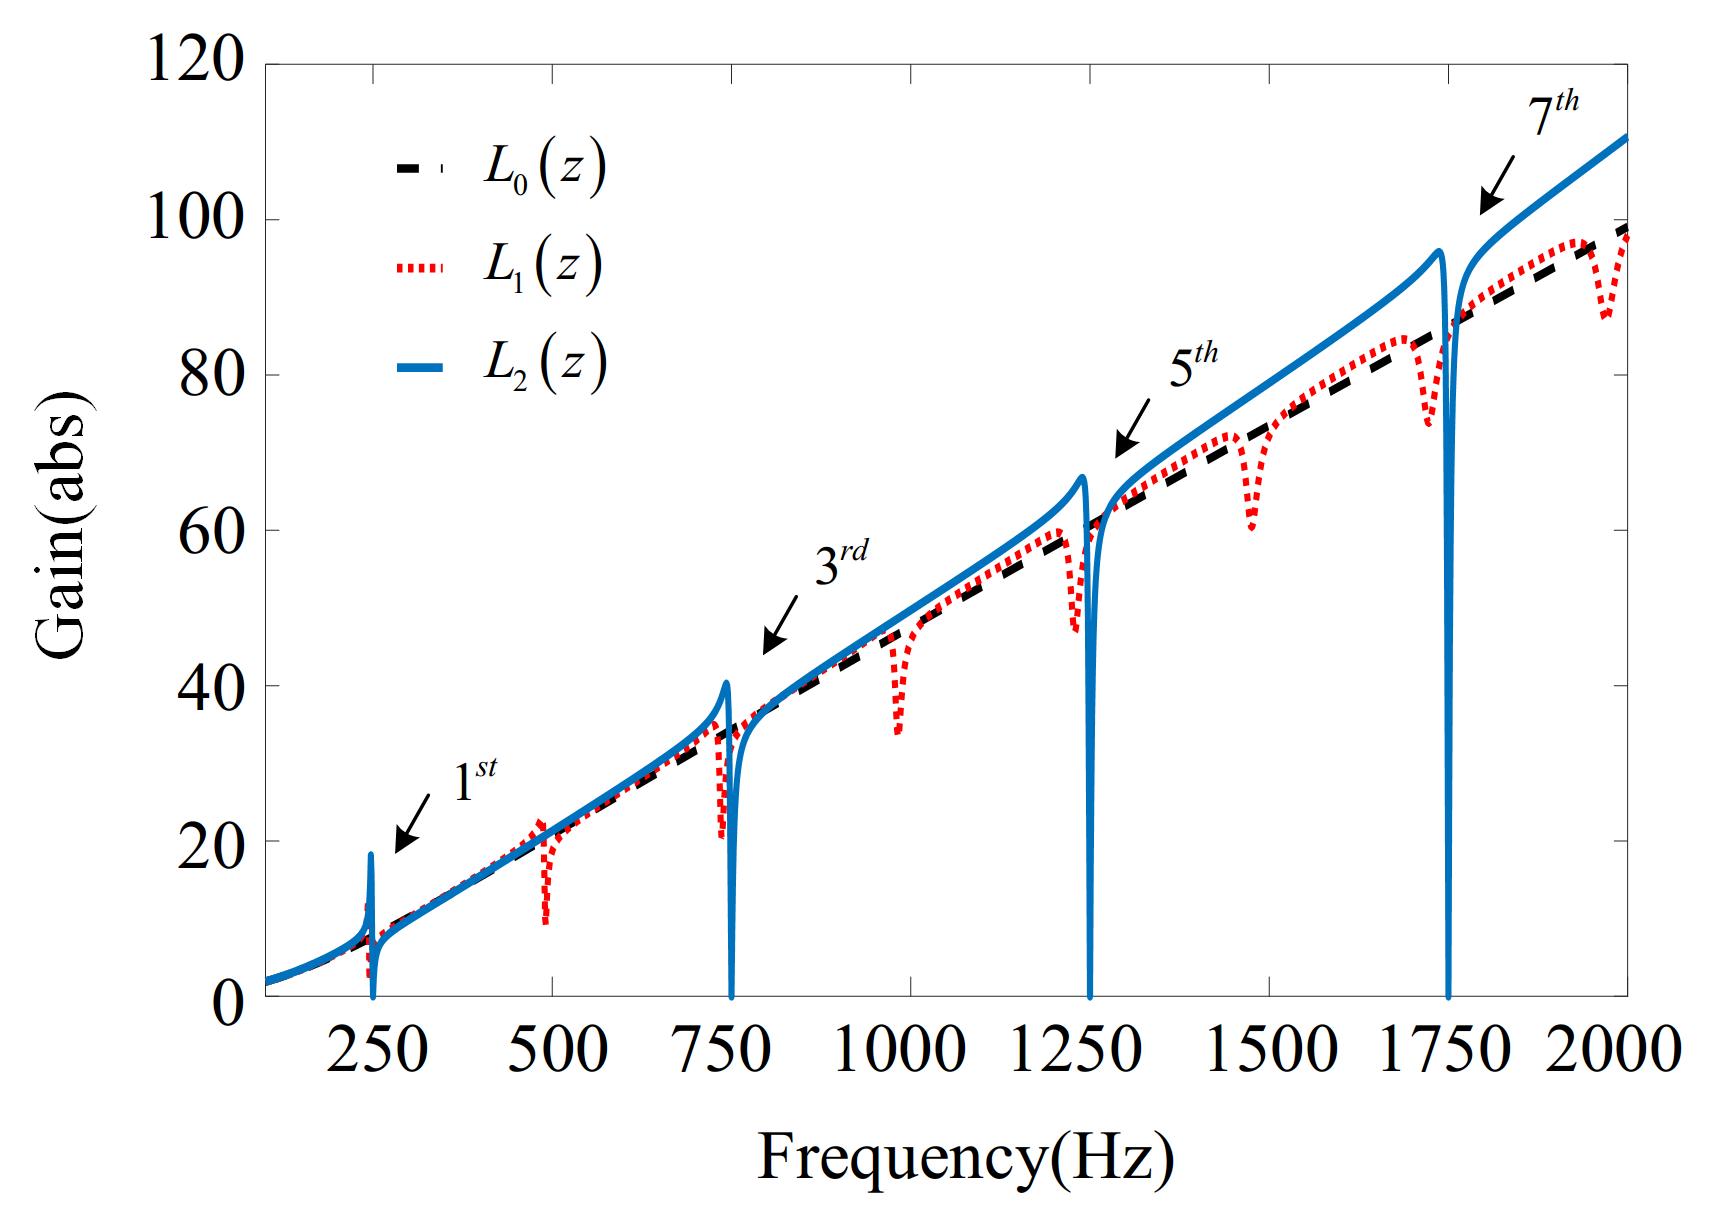
\includegraphics[scale=1.0]{3-sensitivity.png}
	\caption{$L_0(z)$、$L_1(z)$和$L_2(z)$传递函数幅频曲线}
	\label{fig:3-sensitivity}
\end{figure}

\autoref{fig:3-sensitivity}显示了$L_0(z)$、$L_1(z)$和$L_2(z)$传递函数幅频曲线。可以看到,除了凹陷处有差异,$L_0(z)$、$L_1(z)$和$L_2(z)$曲线形状基本一致,表明插入重复控制器并不改变电流传递函数在凹陷频率之外的特性。$L_0(z)$是一个平滑的曲线,因此不插入重复控制器的闭环系统不具备抑制谐波电流的能力。$L_1(z)$和$L_2(z)$在陷波频率处有一定程度的凹陷,因此整数次重复控制器和零相移奇数次重复控制器均可以抑制谐波电流。然而从图中可以看出,随着频率升高,整数次重复控制器的陷波频率逐渐发生偏移250Hz,500Hz,750Hz,..,这使得其谐波抑制能力逐渐下降。此外,其偶数倍于基波频率的陷波频率是没有必要的。与之相对比的是$L_2(z)$的陷波频率均准确定在奇数倍与基波频率处,没有发生偏移,且曲线凹陷程度比$L_1(z)$更深。这使得零相移奇数次重复控制器拥有更优的谐波抑制能力。

\autoref{fig:3-2-crc}和\autoref{fig:orc}所对应的的仿真模型如\autoref{fig:3-simulink_model}所示。在两个模型中注入含有谐波频率一致、各频率谐波的幅值一致的扰动信号,然后同时加入传统整数次重复控制器和零相移奇数次重复控制器,观察加入重复控制器前后控制电流的变化。
\begin{figure}
	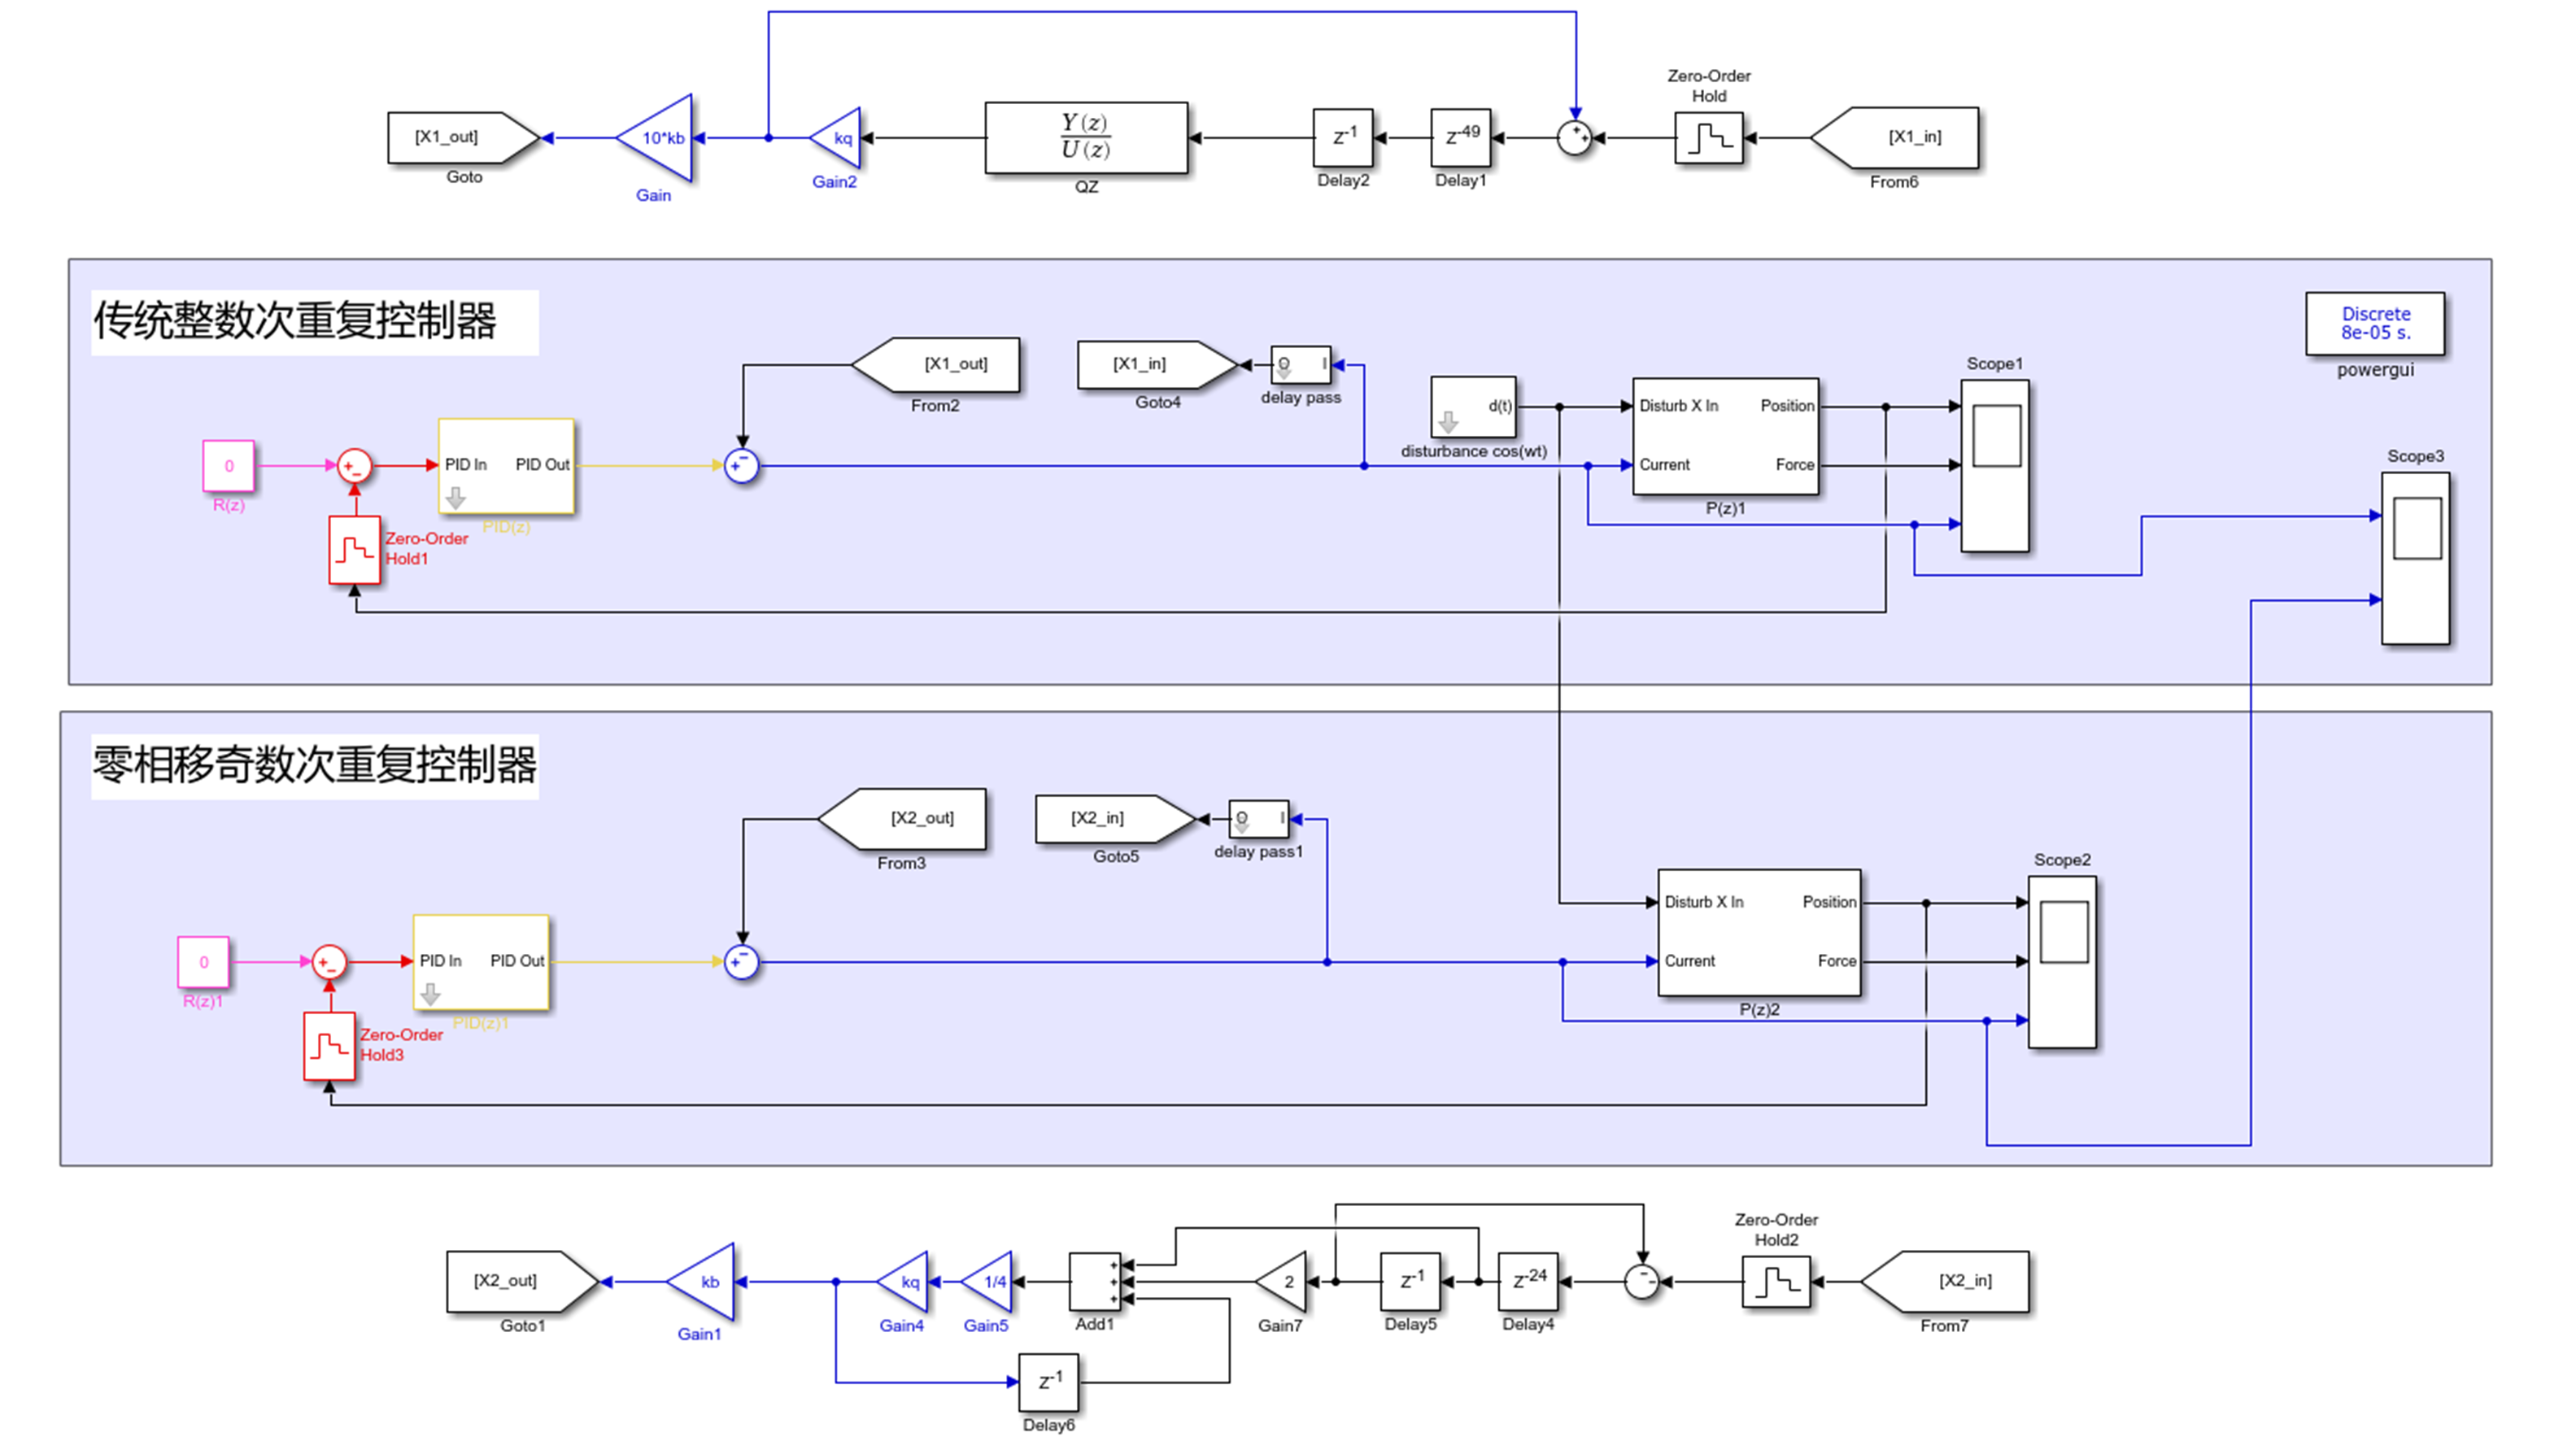
\includegraphics[scale=1.0]{3-simulink_model.png}
	\caption{传统整数次重复控制器和零相移奇数次重复控制器仿真模型}
	\label{fig:3-simulink_model}
\end{figure}

\begin{figure}
	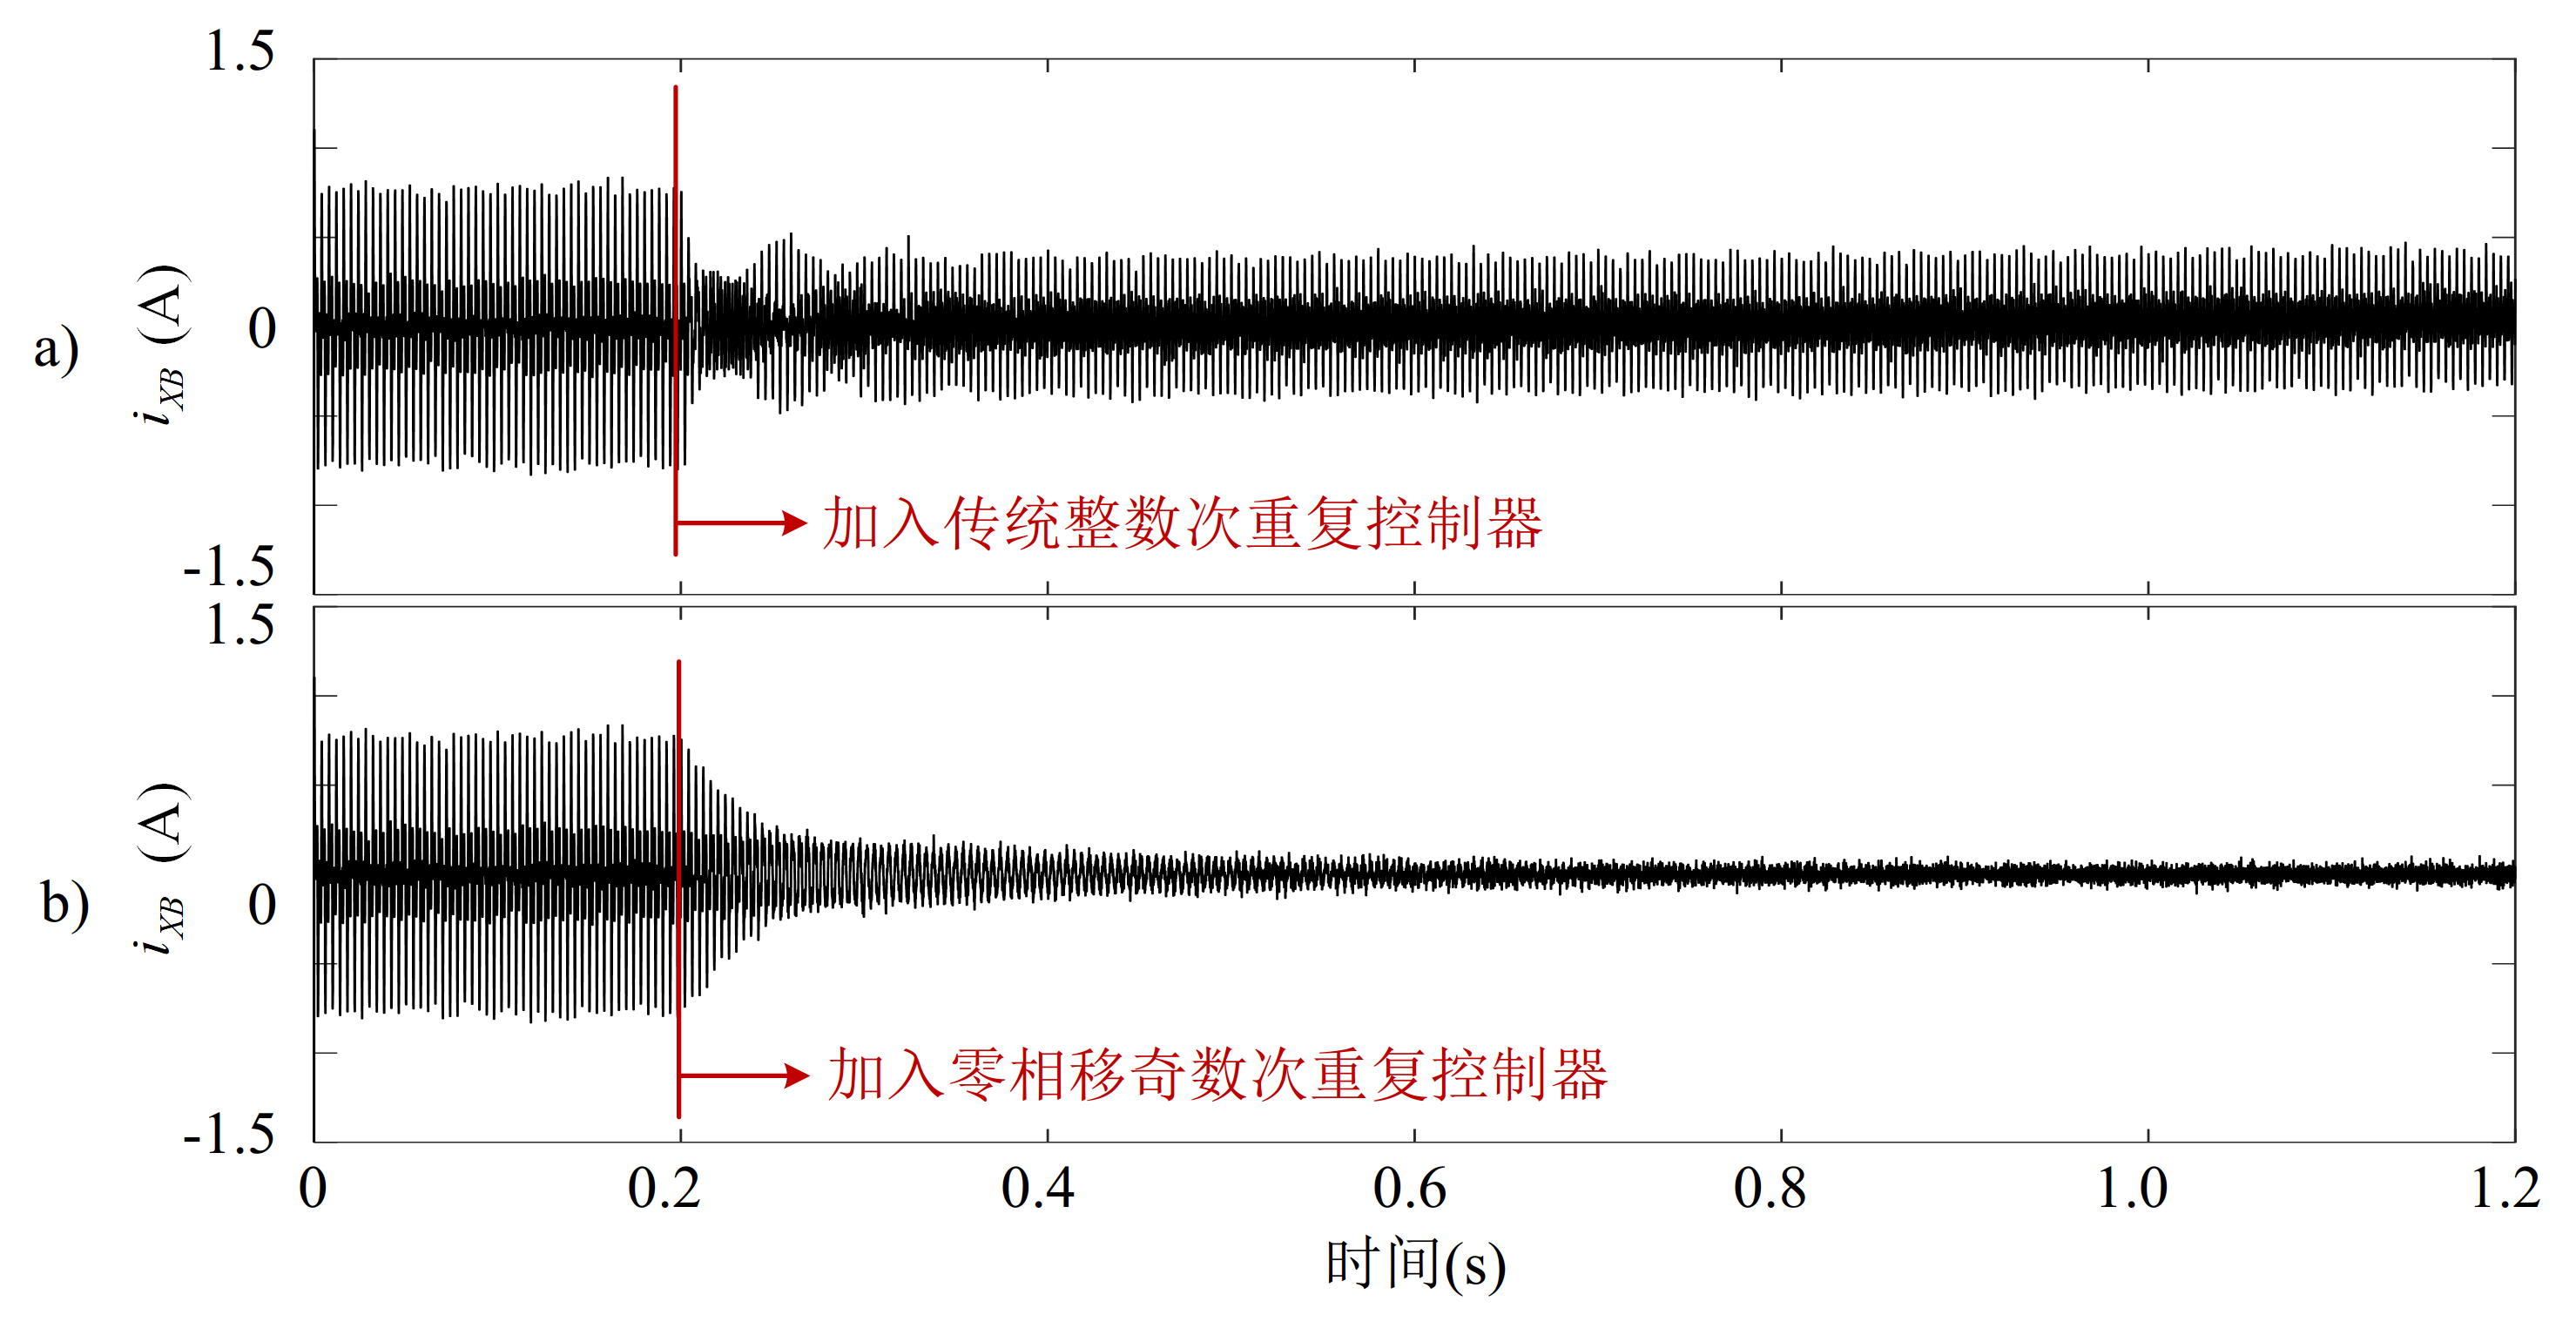
\includegraphics[scale=1.0]{3-current.png}
	\caption{加入传统整数次重复控制器和加入零相移奇数次重复控制器的电流波形}
	\label{fig:3-current}
\end{figure}

从\autoref{fig:3-current}可以看到,加入重复控制器前,扰动信号造成电流中存在幅值约为0.7A的交流成分。加入传统整数次重复控制器后,谐波电流幅值下降到约0.4A;加入零相移奇数次重复控制器后,谐波电流幅值下降到约0.2A。两种情况下转子均未失稳。仿真结果说明零相移奇数次重复控制器可以有效抑制控制电流中的谐波分量,且比传统整数次重复控制器的谐波抑制能力更强。
\section{本章小结}
本章针对传统整数次重复控制器存在相位延迟进而导致其在磁悬浮轴承应用中谐波抑制能力不足的问题,提出了一种新的重复控制器算法——零相移奇数次重复控制器。分析比较了传统整数次重复控制器和零相移奇数次重复控制器的工作原理和稳定性分析方法。最后通过仿真结果验证了零相移奇数次重复控制器拥有更优的谐波抑制性能。
\chapter{基于重复控制器的现场动平衡方法}
本章分析了磁悬浮轴承中转子常用的现场动平衡方法:影响系数法、改进的影响系数法、旋转轴控制法。其中旋转轴控制法无需试重,操作更加简单方便。针对传统的绕惯性轴控制法没有考虑电流谐波抑制的问题,本文提出一种基于谐波抑制的绕惯性轴旋转方案,分析了其中谐波抑制、不平衡质量辨识、校正质量计算步骤。
\section{需试重的现场动平衡方法介绍}
\subsection{影响系数法}

\subsection{改进的影响系数法}

\section{无需试重的现场动平衡方法介绍}
无需试重的现场动平衡方法通常需先辨识转子不平衡质量分布,再通过增重法或去重法补偿转子质量不平衡。其中辨识转子不平衡质量有多种途径实现
:零位移法、零电流法、零力法。三种方法简要介绍见下文。

\subsection{零位移法辨识转子偏心质量分布}

存在初始不平衡质量的转子在旋转时的几何轴、惯性轴和旋转轴不重合,截面视图下,三者位于同一直线上,如\autoref{fig:2-3-sensor}所示。以旋转中心为原点建立平面坐标系,此时不妨认为磁悬浮轴承磁极中心与转子旋转中心是重合的,分析单端的转子运动轨迹方程。
\begin{figure}
	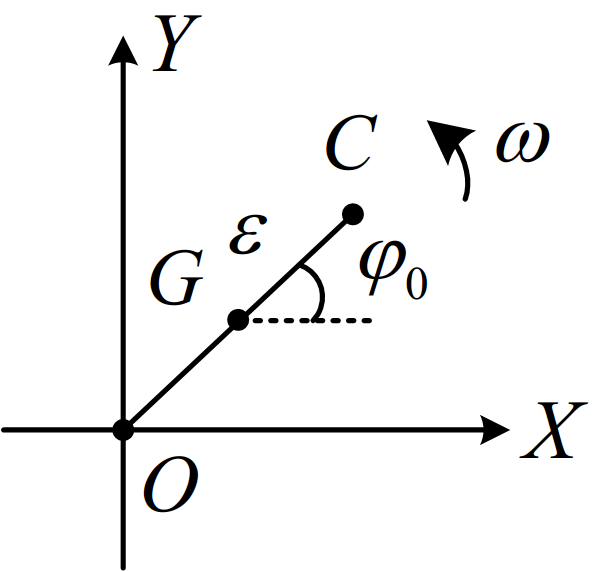
\includegraphics[scale=1.0]{4-geo_axis.png}
	\caption{初始不平衡质量的幅值和相位}
	\label{fig:4-geo_axis}
\end{figure}
\autoref{fig:4-geo_axis}显示了单端初始不平衡质量的幅值和相位的示意图,在该转子转向下,转子在$y$轴的运动滞后$x$轴运动$90^{\circ}$。因此,定义复数信号$z_c$、$z_g$和$z_{\Delta}$分别表示转子的质量中心、几何中心和偏心距。则有
\begin{equation}
z_c = x_c + jy_c
\end{equation}
\begin{equation}
z_g = x_g + jy_g
\end{equation}
\begin{equation}
\label{eq:z_delta}
z_{\Delta} = \varepsilon cos(\omega t+\phi _0) + jsin(\omega t + \phi _0) = \varepsilon e^{j(\omega t + \phi _0)}
\end{equation}
此三个矢量的关系为:
\begin{equation}
	\label{eq:z_c}
	z_c = z_g + z_{\Delta}
\end{equation}
当通过施加某些算法(如陷波器算法)使旋转轴与几何轴重合时,几何中心与坐标原点可视为重合,如\autoref{fig:4-geo_axis_co}所示。其中
\begin{figure}
	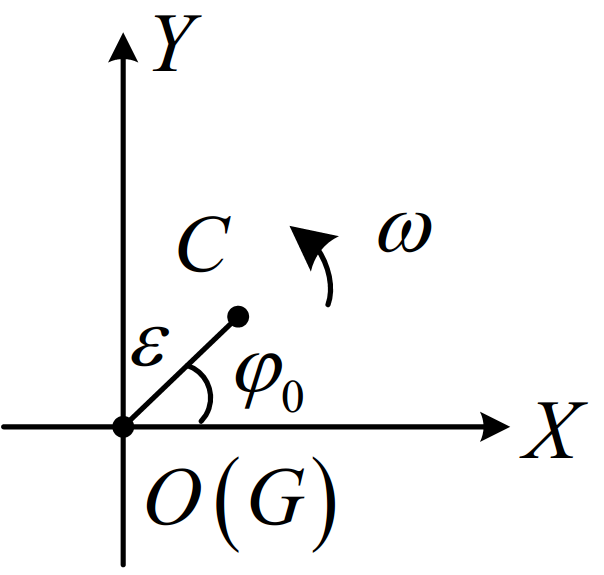
\includegraphics[scale=1.0]{4-geo_axis_co.png}
	\caption{几何中心与旋转中心重合时的不平衡质量的幅值和相位}
	\label{fig:4-geo_axis_co}
\end{figure}
\begin{equation}
	\label{eq:z_g_0x}
	z_g = 0
\end{equation}
磁悬浮轴承中的磁悬浮力为:
\begin{equation}
	\label{eq:f_z}
	f_z = k_ii_z + k_sz_g
\end{equation}
由牛顿第二运动定律可得:
\begin{equation}
	\label{eq:f_z_a}
	f_z = m{\ddot{z}}_c
\end{equation}
联立方程\autoref{eq:z_c},\autoref{eq:z_g_0x},\autoref{eq:f_z}和\autoref{eq:f_z_a}可得
\begin{equation}
	\label{eq:geo_eq}
	-m\varepsilon {\omega}^2e^{j(\omega t + \phi _0)} = k_ii_z
\end{equation}
记电流传感器测得的单端两自由度控制电流波形为
\begin{equation}
	\label{eq:i_z_0x}
	i_z = A_ie^{j(\omega t + \phi _i)}
\end{equation}
则将\autoref{eq:i_z_0x}带入\autoref{eq:geo_eq}可以解出不平衡质量矢量的幅值和相位为
\begin{equation}
\left\{
\begin{aligned}
& \varepsilon = \frac{k_iA_i}{m{\omega}^2}\\
& \phi _0 = \phi _i + \pi
\end{aligned}
\right.
\end{equation}


\subsection{零力法辨识转子偏心质量分布}

绕惯性轴旋转通常有两种控制策略:零力控制和零电流控制。前者是指使用振动力控制算法完全抑制磁悬浮振动力,使旋转轴和惯性轴完全重合;后者是指使用振动电流控制算法抑制磁悬浮轴承线圈中的振动电流,使旋转轴趋于惯性轴。

零力控制下磁悬浮力为零(竖直方向上仍存在直流偏置的磁悬浮力抵消重力,此处仅需研究磁悬浮力交流分量),即
\begin{equation}
	\label{eq:f_z_0f}
	f_z = 0
\end{equation}
此时单端转子质量中心与旋转中心完全重合,如\autoref{fig:4-ine_axis_co}所示。其中
\begin{equation}
	\label{eq:z_c_0f}
	z_c = 0
\end{equation}
记位移传感器测得的单端转子位移波形为
\begin{equation}
	\label{eq:z_g_0f}
	z_g = A_ze^{j(\omega t + \phi _z)}
\end{equation}
联立\autoref{eq:z_c}、\autoref{eq:z_c_0f}和\autoref{eq:z_g_0f}即可得到不平衡质量矢量的幅值和相位
\begin{equation}
\left\{
\begin{aligned}
& \varepsilon = A_z\\
& \phi _0 = \phi _z
\end{aligned}
\right.
\end{equation}

\begin{figure}
	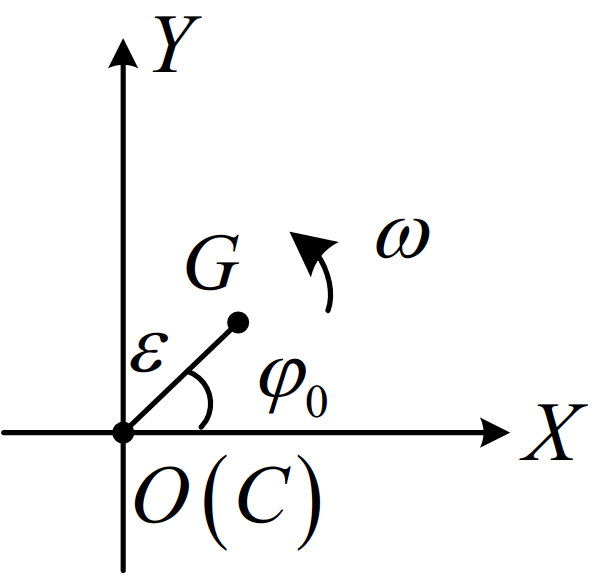
\includegraphics[scale=1.0]{4-ine_axis_co.png}
	\caption{质量中心与旋转中心重合时的不平衡质量的幅值和相位}
	\label{fig:4-ine_axis_co}
\end{figure}


\subsection{零电流法辨识转子偏心质量分布}

零电流控制是加入算法抑制电流中的同频分量,使得电流中的扰动信号的基波趋近于零,记为
\begin{equation}
	\label{eq:i_z_0i}
	i_z = 0
\end{equation}
联立\autoref{eq:z_c}、\autoref{eq:z_c_0f}和\autoref{eq:i_z_0i},可得
\begin{equation}
	\label{eq:0i_eq}
	m{\ddot{z}}_g - m{\omega}^2\varepsilon e^{j (\omega t + \phi _0)} = k_sz_g 
\end{equation}
解该微分方程即可得到
\begin{equation}
	\label{eq:z_g_0i}
	z_g = \frac{\varepsilon}{1-\frac{k_s}{m{\omega}^2}}
\end{equation}
联立\autoref{eq:z_g_0f}和\autoref{eq:z_g_0i},可以解出不平衡质量矢量的幅值和相位分别为:
\begin{equation}
\label{eq:z_delta_0i}
\left\{
\begin{aligned}
& \varepsilon = A_z\left( 1 -\frac{k_s}{m{\omega}^2} \right) \\
& \phi _0 = \phi _z
\end{aligned}
\right.
\end{equation}

通过以上的原理介绍可以看出,无需试重即可使用以上三种方法之一辨识出转子不平衡质量分布。根据辨识出的不平衡质量分布,即可计算出校正质量来进行不平衡质量补偿。计算校正质量的详细步骤见本章后文所述。

\section{基于重复控制器的现场动平衡方法}

\subsection{实现零电流控制}

一、传统方案:使用陷波器法实现零电流控制

陷波器是磁悬浮轴承振动抑制研究中常用的同频振动抑制策略。当其用于抑制电流中的同频振动成分以消除磁悬浮轴承振动力时,陷波器被以反馈的形式插入到闭环控制回路中。若以$N_f(s)$表示陷波器的开环传递函数,则插入陷波器的闭环系统控制框图如\autoref{fig:4-nfz}所示。

\begin{figure}
	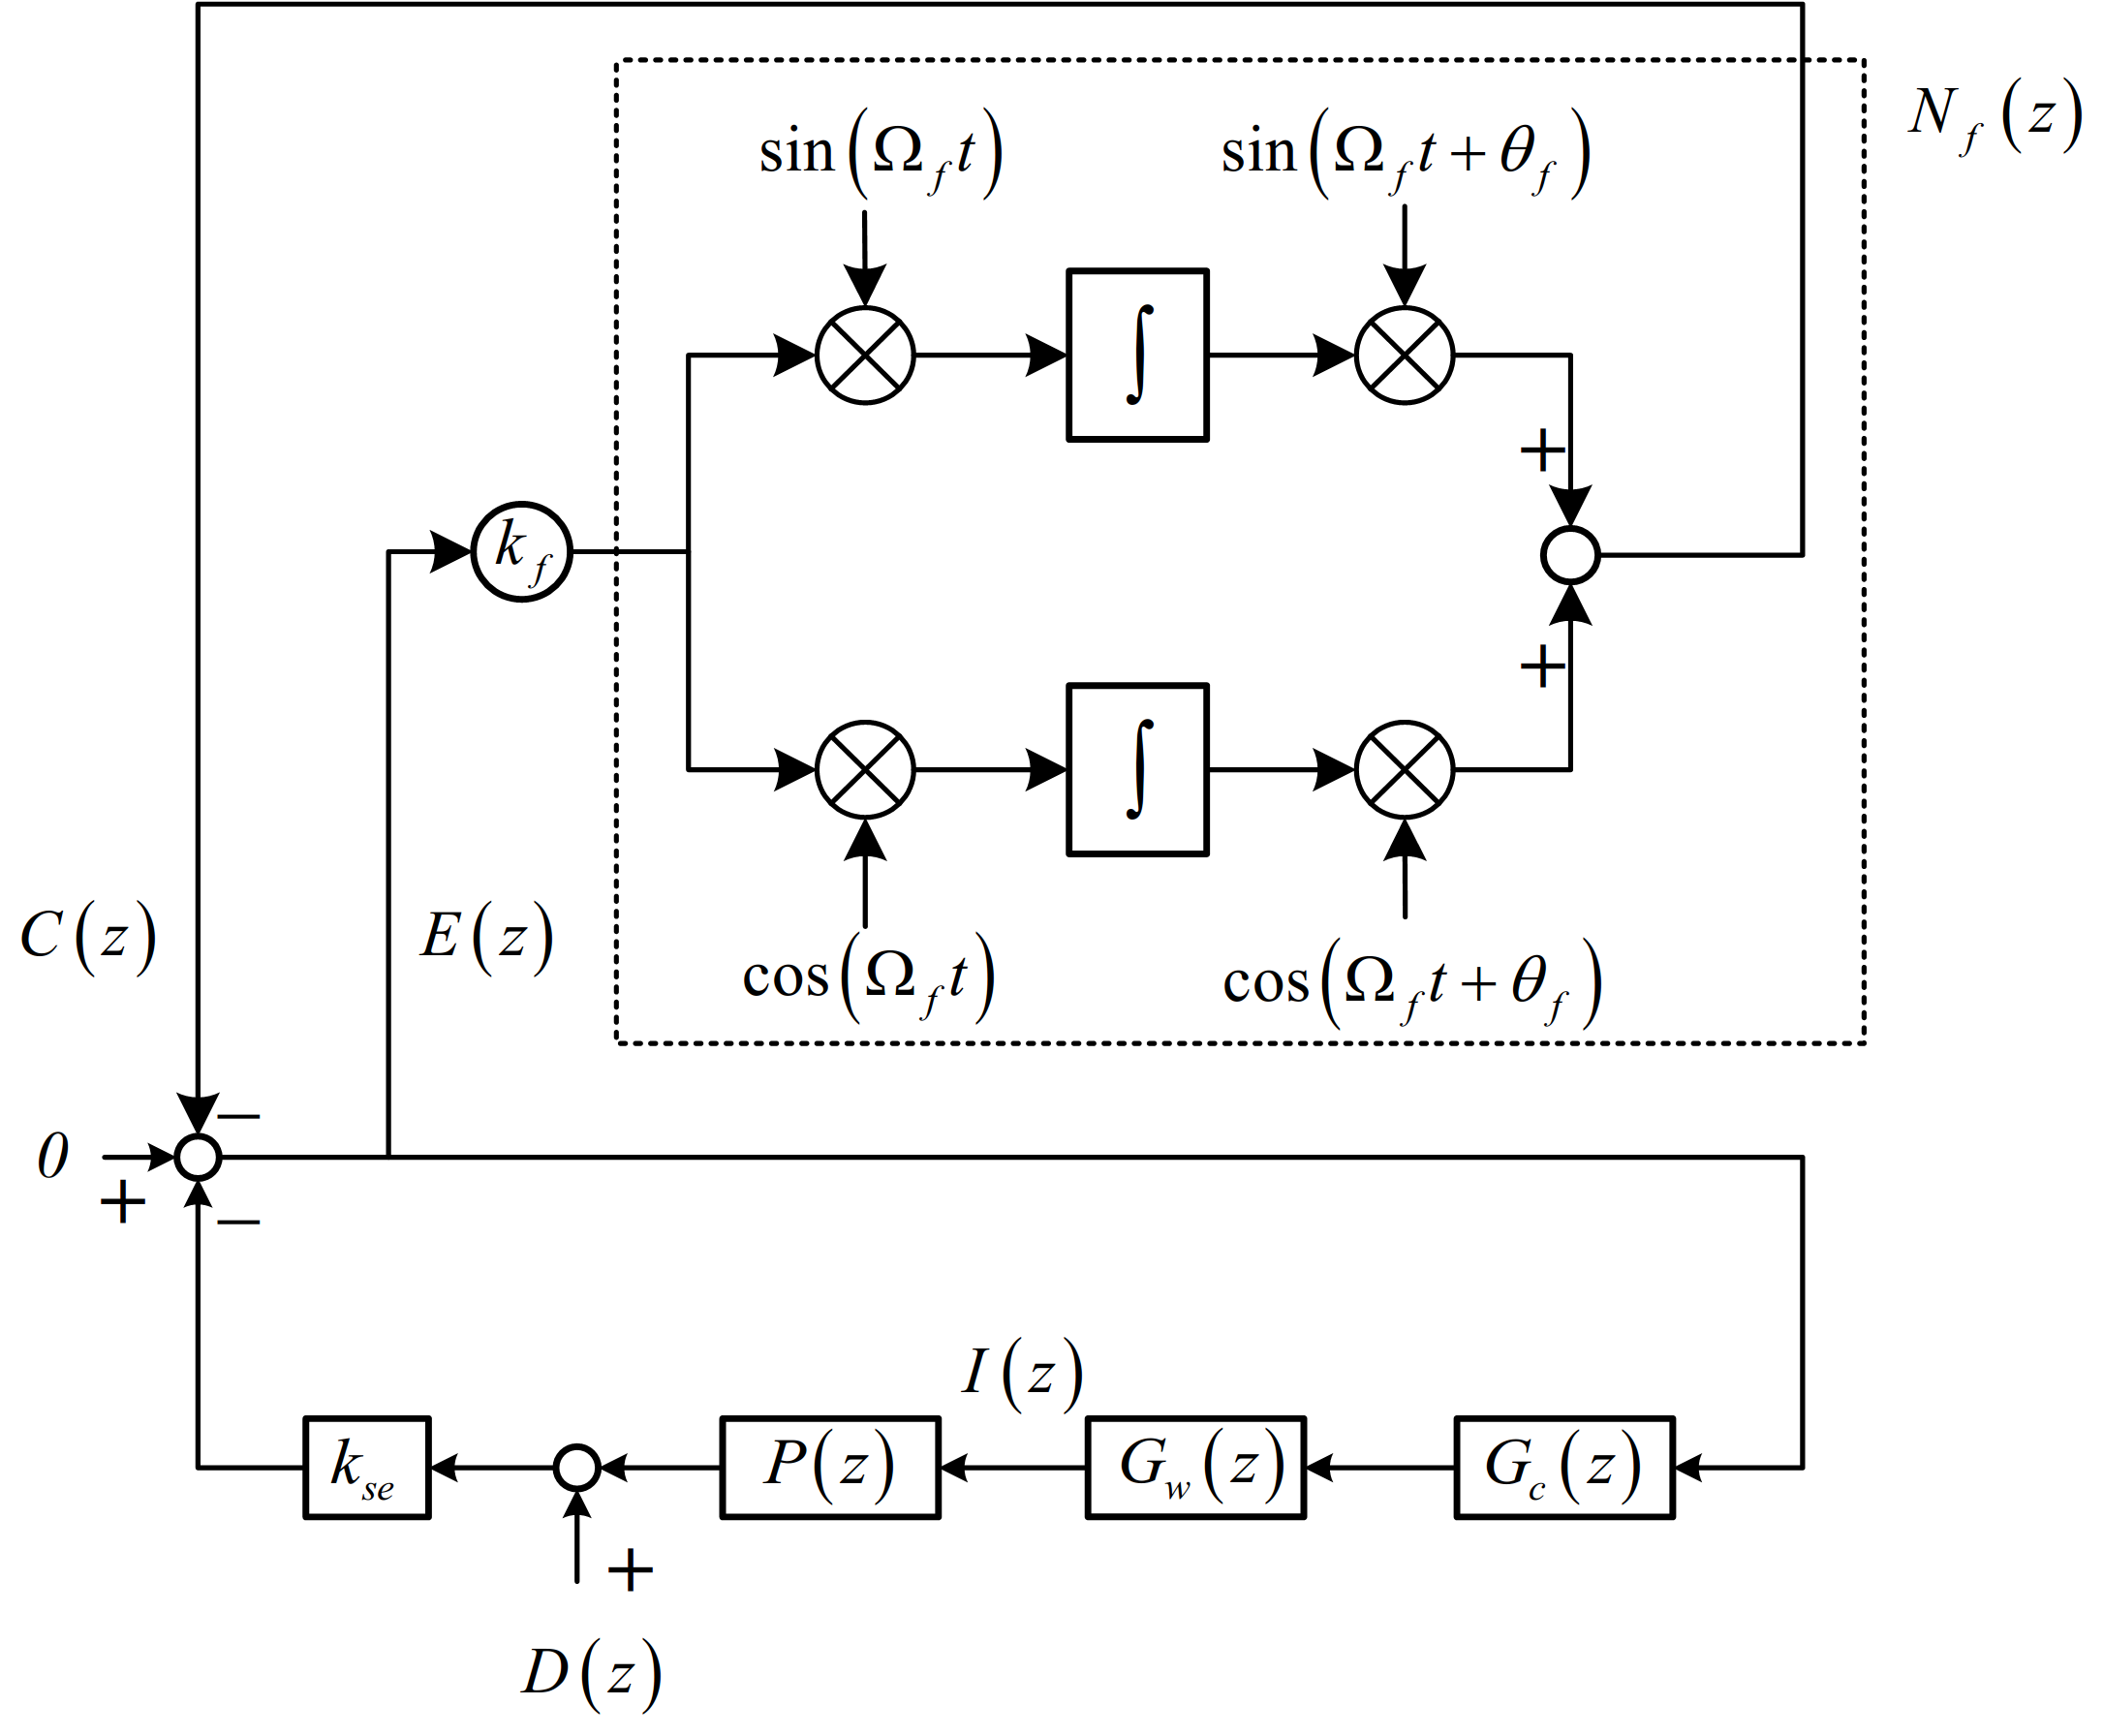
\includegraphics[scale=1.0]{4-nfz.png}
	\caption{插入陷波器的闭环系统控制框图}
	\label{fig:4-nfz}
\end{figure}

图中,$k_f$是指陷波器增益,$\theta$指陷波器相位角,$\Omega$是陷波频率,为抑制同频振动力,此处陷波频率选取为转子转动频率。陷波器的输入信号包括转子位移误差信号$e(t)$(对应图中$E(z)$)和一对相位相差$90^{\circ}$的标准正弦信号,输出信号为$c(t)$(对应图中$C(z)$)。其信号处理规律推导如下:
\begin{equation}
c(t) = sin(\Omega t + \theta _f) \int [sin(\Omega t)e(t)]+cos(\Omega t + \theta _f) \int [cos(\Omega t)e(t)]
\end{equation}
对上式两端同时对$t$求二次导数,可以得到
\begin{equation}
\ddot{c}(t) = -{\Omega}^2c(t)+cos(\theta _f)\dot{e}(t)-\Omega sin(\theta _f)e(t)
\end{equation}
对上式进行拉普拉斯变换得到:
\begin{equation}
s^2C(s) = -{\Omega}^2C(s)+scos(\theta _f)E(s)-\Omega sin(\theta _f)E(s)
\end{equation}
由此得到陷波器的开环传递函数$N_f(s)$为:
\begin{equation}
N_f(s) = \frac{C(s)}{E(s)} = \frac{scos(\theta _f) - \Omega sin(\theta _f)}{s^2 + {\Omega}^2}
\end{equation}
那么陷波器的闭环传递函数$N(s)$为:
\begin{equation}
N(s) = \frac{1}{1+k_fN_f(s)}=\frac{s^2+{\Omega}^2}{s^2+k_fcos(\theta _f)s + {\Omega}^2-k_f\Omega sin(\theta _f)}
\end{equation}

加入该陷波器可以使同频电流的幅值完全消除,同时依据该文献给出的插入陷波器的闭环控制回路的稳定性分析方法,陷波器的参数$k_f$和$\theta _f$的选取原则为(【此处待添加引用何家希硕士论文】):
\begin{enumerate}
	\item $\theta _f = - arg\left[ S_0(j\Omega) \right]$,其中$S_0$为该自由度的输出敏感度函数;
	\item $k_f$越大,误差收敛速度越快,但是系统稳定性越差。实验过程中应该根据实验现象由小至大选取合适的$k_f$值。
\end{enumerate}


二、新型方案:使用零相移奇数次重复控制器实现零电流控制

位移传感器引入的谐波扰动使得控制电流中包含不仅包含质量不平衡引起的与转速同频的扰动,也包含谐波成分。使用传统的陷波器抑制同频振动电流后,其剩下的控制电流可以表示为:
\begin{equation}
	\label{eq:iz_0i_h}
	{i} = \sum\limits_{n = 2}^\infty  {{A_{ni}}{e^{j(n\omega t + {\varphi _{ni}})}}} 
\end{equation}
电流中的交流分量并不为零。对于基于零电流控制的转子偏心质量辨识方法而言,辨识结果准确度则无法保证。本文使用第三章提出的奇数次零相移重复控制器方法,同时消除控制电流中的同频分量和谐波分量,消除电流中的交流分量,实现零电流控制。

奇数次零相移重复控制器的参数设计和实验步骤如第三章和第五章所述,此处不再赘述。

\subsection{辨识不平衡质量}

考虑振动力的转子动力学方程为
\begin{equation}
M\left( {{{\ddot q}_g} + {{{\ddot q}}_\Delta }} \right) + G\left( {{{\dot q}_{g}} + {{{\dot q}}_\Delta }} \right) = {B}{K_x}{{B}^{T}}{{q}_g} + {B}{{K}_{i}}{i}
\end{equation}
当控制电流的交流分量为零时,上式重写为
\begin{equation}
M\left( {{{\ddot q}_g} + {{{\ddot q}}_\Delta }} \right) + G\left( {{{\dot q}_{g}} + {{{\dot q}}_\Delta }} \right) = {B}{K_x}{{B}^{T}}{{q}_g}
\end{equation}
进行拉普拉斯变换后可得
\begin{equation}
\left( {M{s^2} + Gs} \right)\left[ {{q_g}\left( s \right) + {q_\Delta }\left( s \right)} \right] =  B{{K}_{s}}{{B}^{T}}{{q}_g}\left( s \right)
\end{equation}
其中
\begin{equation}
{B}{K_s}{{B}^{T}} = \left[ {\begin{matrix}
   {l_{bA}^2 + l_{bB}^2} & { - {l_{bA}} + {l_{bB}}} & 0 & 0  \cr 
   { - {l_{bA}} + {l_{bB}}} & 2 & 0 & 0  \cr 
   0 & 0 & {l_{bA}^2 + l_{bB}^2} & { - {l_{bA}} + {l_{bB}}}  \cr 
   0 & 0 & { - {l_{bA}} + {l_{bB}}} & 2  \cr 
 \end{matrix} } \right]
\end{equation}
当两端磁极到中心距离一致,即${l_{bA}} = {l_{bB}} = {l_b}$时,上式可以化简为:
\begin{equation}
\label{eq:sys_b}
{B}{K_s}{{B}^{T}} = \left[ {\begin{matrix}
   {2l_b^2} & 0 & 0 & 0  \cr 
   0 & 2 & 0 & 0  \cr 
   0 & 0 & {2l_b^2} & 0  \cr 
   0 & 0 & 0 & 2  \cr 

 \end{matrix} } \right]
\end{equation}
转子径向上的运动分为平动——$x$和$y$运动和转动——$\alpha$和$\beta$。在\autoref{eq:sys_b}所示的条件下,径向上的平动和转动可以解耦分析。定义复数信号$\eta _g(t)$和$\nu _g(t)$分别表示转子几何中心的平动位移和转动位移,复数信号$\eta _{\Delta}(t)$和$\nu _{\Delta}(t)$分别表示偏心质量的平动位移和转动位移,其可以表示为:
\begin{equation}
\label{eq:decouple_define}
\left\{
\begin{aligned}
& \eta _g(t) = x_g(t) + jy_g(t)\\
& \eta _{\Delta}(t) = x_{\Delta}(t) + jy_{\Delta}(t)\\
& \nu _g(t) = {\beta}_g(t) - j{\alpha}_g(t)\\
& \nu _{\Delta}(t) = {\beta}_{\Delta}(t) - j{\alpha}_{\Delta}(t)\\
\end{aligned}
\right.
\end{equation}
根据\autoref{eq:q_delta}定义,转子平动和转动方向上的不平衡质量分别为:
\begin{equation}
\label{eq:eta_nu_define}
\left\{
\begin{aligned}
&\eta _{\Delta}(t) = ee^{j(\omega t + \theta)} \\
&\nu _{\Delta}(t) = \sigma e^{j(\omega t + \gamma)} \\
\end{aligned}
\right.
\end{equation}
在不影响实际实验准确性的前提下,我们假设:
\begin{enumerate}
	\item 转子径向对称:$I_x = I_y = I_r$;
	\item 忽略细长转子的陀螺效应,即认为$G = 0$
\end{enumerate}
则\autoref{eq:sys_b}和\autoref{eq:decouple_define}可以重写为:
\begin{equation}
\label{eq:decouple}
\left\{
\begin{aligned}
& ms^2\left[ \eta _g(s)+\eta_{\Delta}(s) \right] = 2k_s\eta _g(s)\\
& {I_r}s^2\left[ \nu _g(s)+\nu_{\Delta}(s) \right] = 2k_s{l_b}^2\nu _g(s)\\
\end{aligned}
\right.
\end{equation}
\autoref{eq:decouple}可以解出:
\begin{equation}
\label{eq:cofficient}
\left\{
\begin{aligned}
& \eta _g (t) = -\frac{m{\Omega}^2}{m{\Omega}^2+2k_s}\eta _{\Delta}(t)\\
& \nu _g (t) = -\frac{I_r{\Omega}^2}{I_r{\Omega}^2+2k_s{l_b}^2}\nu _{\Delta}(t)\\
\end{aligned}
\right.
\end{equation}
由\autoref{eq:cofficient}可以看出,得到$\eta _g(t)$和$\nu _g(t)$的信息才能得到不平衡质量的幅值和相位。但是如前文所提到,由于传感器误差的存在,转子几何中心无法测得。考虑到与质量不平衡的幅值相比,传感器误差的幅值要小得多,保持不妨假设
\begin{equation}
\label{eq:assumption}
\left\{
\begin{aligned}
& \eta _g (t) = \eta _s (t)\\
& \nu _g (t) = \nu _s (t)  \\
\end{aligned}
\right.
\end{equation}
$\eta _s$和$\nu _s$可以通过位移传感器采集得到,其可以表示为
\begin{equation}
\label{eq:eta_s}
\left\{
\begin{aligned}
& \eta _s (t) = A_{\eta}e^{j(\omega t + \phi _{\eta})} \\
& \nu _s (t) = A_{\nu}e^{j(\omega t + \phi _{\nu})} \\
\end{aligned}
\right.
\end{equation}
联立\autoref{eq:eta_nu_define}、\autoref{eq:cofficient}和\autoref{eq:eta_s},可以解得不平衡质量矢量的幅值和相位为:
\begin{equation}
\left\{
\begin{aligned}
& e = A_{\eta}\frac{m{\Omega}^2 + 2k_s}{m{\Omega}^2}\\
& \sigma = A_{\nu}\frac{I_r{\Omega}^2 + 2k_s{l_b}^2}{I_r{\Omega}^2}\\
\end{aligned}
\right.
\end{equation}
通过转角传感器辨识双端位移波形相位,即可获取平动和转动方向的不平衡质量初相位$\theta$和$\gamma$。
\subsection{计算校正质量}
辨识出不平衡质量矢量的幅值和相位之后,通过在双端配重盘增重的方式来补偿转子初始不平衡质量。记在补偿盘A上的增重质量为$m_A$,相位为$\phi _A$;补偿盘B上的增重质量为$m_B$,相位为$\phi _B$。则补偿力矩矩阵可以表示为:
\begin{equation}
Q_c = T_cM_c
\end{equation}
其中
\begin{equation}
{M_c}{\rm{ = }}\left[ {\begin{matrix}
   {{m_a}{r_a}\cos \left( {{\varphi _A}} \right)}  \cr 
   {{m_b}{r_b}\cos \left( {{\varphi _B}} \right)}  \cr 
   {{m_a}{r_a}\sin \left( {{\varphi _A}} \right)}  \cr 
   {{m_b}{r_b}\sin \left( {{\varphi _B}} \right)}  \cr 

 \end{matrix} } \right]
\end{equation}
\begin{equation}
{T_c} = \left[ {\begin{matrix}
   { - {l_{cA}}} & {{l_{cB}}} & 0 & 0  \cr 
   1 & 1 & 0 & 0  \cr 
   0 & 0 & { - {l_{cA}}} & {{l_{cB}}}  \cr 
   0 & 0 & 1 & 1  \cr 

 \end{matrix} } \right]
\end{equation}

增重方式补偿目标为转子合力矩为零,即
\begin{equation}
\label{eq:com_tar}
Mq_{\Delta}{\omega}^2 + Q_cT_c{\omega}^2 = 0
\end{equation}
解\autoref{eq:com_tar}时,先令增重质量分布于正交方向($x$和$y$)上,表示为
\begin{equation}
{M_c}{\rm{ = }}\left[ {\begin{matrix}
   {{m_{ax}}{r_a}}  \cr 
   {{m_{bx}}{r_b}}  \cr 
   {{m_{ay}}{r_a}}  \cr 
   {{m_{by}}{r_b}}  \cr 

 \end{matrix} } \right]
\end{equation}
求出$T_c$的逆矩阵为:
\begin{equation}
{T_c}^{ - 1} = {1 \over {{l_{cA}} + {l_{cB}}}}\left[ {\begin{matrix}
   { - 1} & {{l_{cB}}} & 0 & 0  \cr 
   1 & {{l_{cA}}} & 0 & 0  \cr 
   0 & 0 & { - 1} & {{l_{cB}}}  \cr 
   0 & 0 & 1 & {{l_{cA}}}  \cr 

 \end{matrix} } \right]
\end{equation}
则可以解出正交方向上的不平衡质量分布为:
\begin{equation}
\left[ {\begin{matrix}
   {{m_{ax}}}  \cr 
   {{m_{bx}}}  \cr 
   {{m_{ay}}}  \cr 
   {{m_{by}}}  \cr 

 \end{matrix} } \right] =  - {1 \over {{l_{cA}} + {l_{cB}}}}\left[ {\begin{matrix}
   { - 1} & {{l_{cB}}} & 0 & 0  \cr 
   1 & {{l_{cA}}} & 0 & 0  \cr 
   0 & 0 & { - 1} & {{l_{cB}}}  \cr 
   0 & 0 & 1 & {{l_{cA}}}  \cr 

 \end{matrix} } \right]\left[ {\begin{matrix}
   {{I_r}\sigma \cos \gamma }  \cr 
   {m\varepsilon \cos \theta }  \cr 
   {{I_r}\sigma \sin \gamma }  \cr 
   {m\varepsilon \sin \theta }  \cr 

 \end{matrix} } \right]{\left[ {\begin{matrix}
   {{r_a}}  \cr 
   {{r_b}}  \cr 
   {{r_a}}  \cr 
   {{r_b}}  \cr 

 \end{matrix} } \right]^{ - 1}}
\end{equation}
得到补偿质量幅值和相位为:
\begin{equation}
\left\{
\begin{aligned}
&{m_a} = \sqrt {m_{ax}^2 + m_{ay}^2}\\
&{m_b} = \sqrt {m_{bx}^2 + m_{by}^2} \\  
&{\varphi _A} = \arctan {{{m_{ay}}} \over {{m_{ax}}}} \\
&{\varphi _B} = \arctan {{{m_{by}}} \over {{m_{bx}}}} \\ 
\end{aligned}
\right.
\end{equation}

\section{本章小结}
本章分析了两类磁悬浮轴承现场动平衡方法:需试重和无需试重的现场动平衡方法,理论分析说明绕几何轴旋转方案和绕惯性轴旋转方案均可以无需试重就解析出转子不平衡质量矢量。理论分析表明:考虑位移传感器引入的谐波时,绕几何轴旋转控制的方案的解析精度不受影响,但是绕惯性轴旋转控制的方案中的解析模型不再成立,导致解析精度下降。本章提出基于前文零相移奇数次重复控制器方案,解决位移传感器谐波对绕惯性轴旋转控制方案解析模型的影响,提高了传统方案的解析精度。


\chapter{磁悬浮轴承数字控制平台的实验研究}
磁悬浮轴承系统包含机械部分:磁悬浮轴承及其支撑的转子,和控制部分——控制板卡和控制软件程序。本章将介绍控制板卡的硬件设计和软件设计,进行磁悬浮轴承系统灵敏度函数测定,针对第三章提出的奇数次重复控制器算法进行实验验证,以及针对第四章提出的现场动平衡算法进行实验验证。

\section{硬件设计}
磁悬浮轴承系统硬件部分包括位移传感器、控制板卡和功率放大器,其结构与数据交互关系如\autoref{fig:5-component}所示。
\begin{figure}
	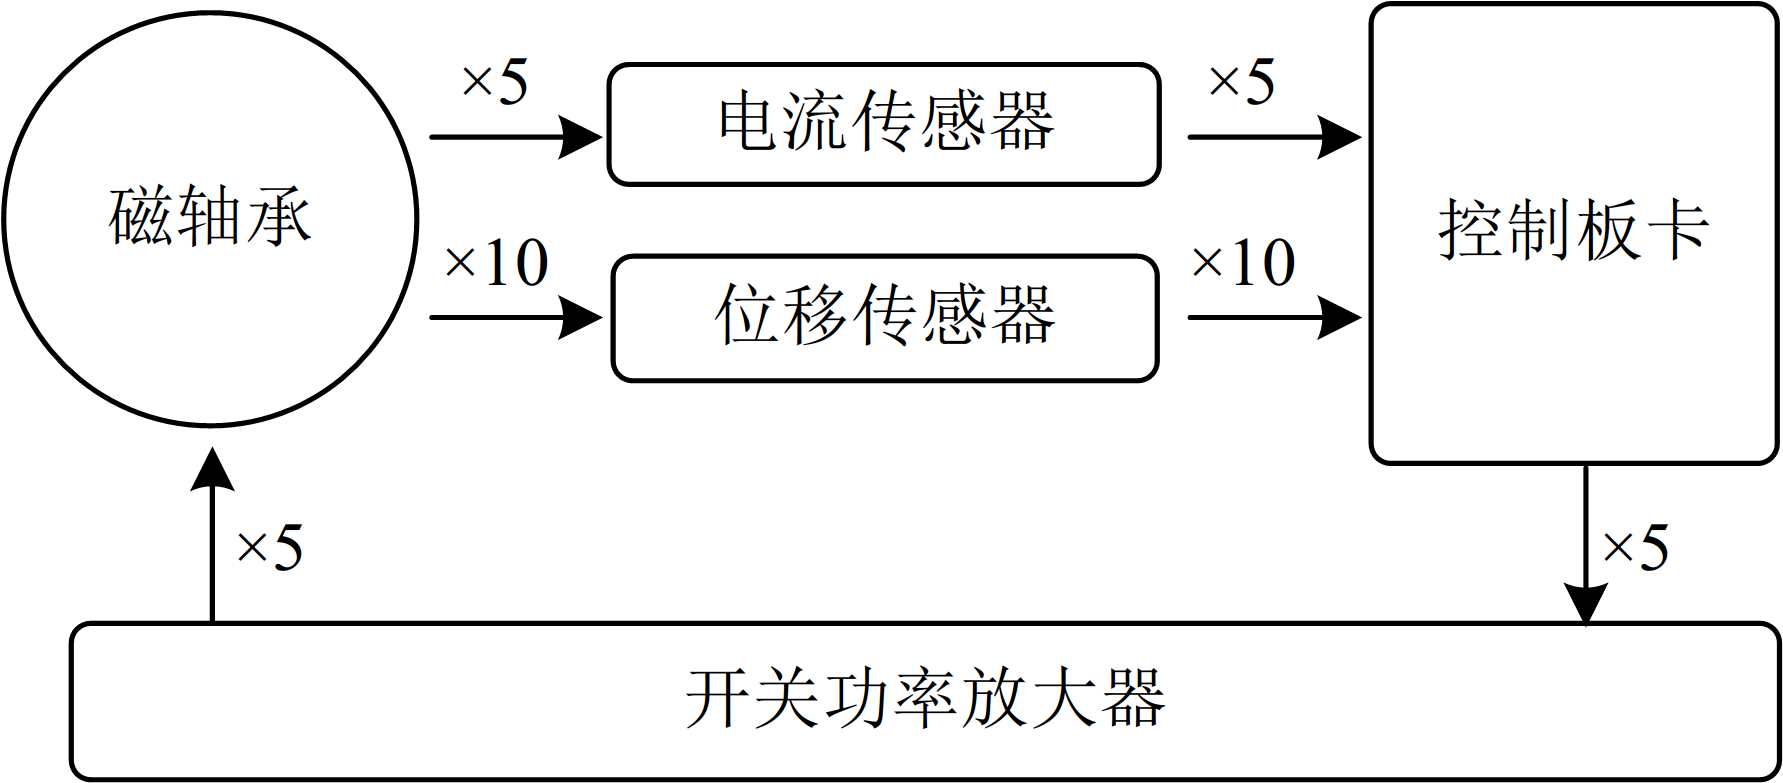
\includegraphics[scale=1.0]{5-component.png}
	\caption{磁悬浮轴承系统硬件组成}
	\label{fig:5-component}
\end{figure}

1.位移传感器

位移传感器用于实时采集转子位置,作为反馈量输入到控制器中。位移传感器的信号质量直接决定了闭环系统控制性能。本文采用电涡流位移传感器,其测量线性范围是$0.10 \sim 1.10mm$,标准灵敏度为$20.00V/mm$,非线性度为$0.8\%$。位移传感器将转子位移量转换成电压输出,经模数转换芯片(ADC)采样后即得到数字量输出。本文使用的ADC芯片输入范围$-10V \sim 10V$,对应输出范围为$-32768 \sim 32767$。则实际位移值到ADC采样数字量之间的系数关系为:
\begin{equation}
\frac{ADC_{reading}}{Displacement} = \frac{20.00V}{1 \times 10^{-3}m} \times \frac{32767}{10V} = 6.5534 \times 10^6/m
\end{equation}

2.电流传感器

电流传感器用于实时采样磁轴承线圈电流值,作为反馈量输入到控制器中。本文研究的磁悬浮离心压缩机用的磁悬浮轴承的额定电流是$-6A\sim 6A$,采用电阻采样式电流传感器。采样电阻阻值为$31m\Omega$,经一级隔离运算放大器放大8.2倍,再经过一级运算放大器放大10倍后,输入到ADC芯片进行采样。实际电流值到ADC采样数字量之间的系数关系为:
\begin{equation}
\frac{ADC_{reading}}{Current} = 31 \times 10^{-3}V \times 8.2 \times 10 \times \frac{32767}{10V} \times \frac{1}{1A} = 8329.4/A
\end{equation}

3.开关功率放大器

开关功率放大器是磁悬浮轴承执行部件之一,其将控制算法输出的参考电流转换成实际线圈电流,使得线圈可以产生磁悬浮力。本文采用全桥式开关功率放大器,母线电压选取为$50V$。五自由度线圈控制共需五组拓扑一致的全桥电路,其中一路全桥电路如\autoref{fig:5-amplifier}所示。基于滞环控制方案使开关管Q1、Q4和Q2、Q3轮流导通,来控制磁轴承线圈电流值跟踪电流给定值。
\begin{figure}
	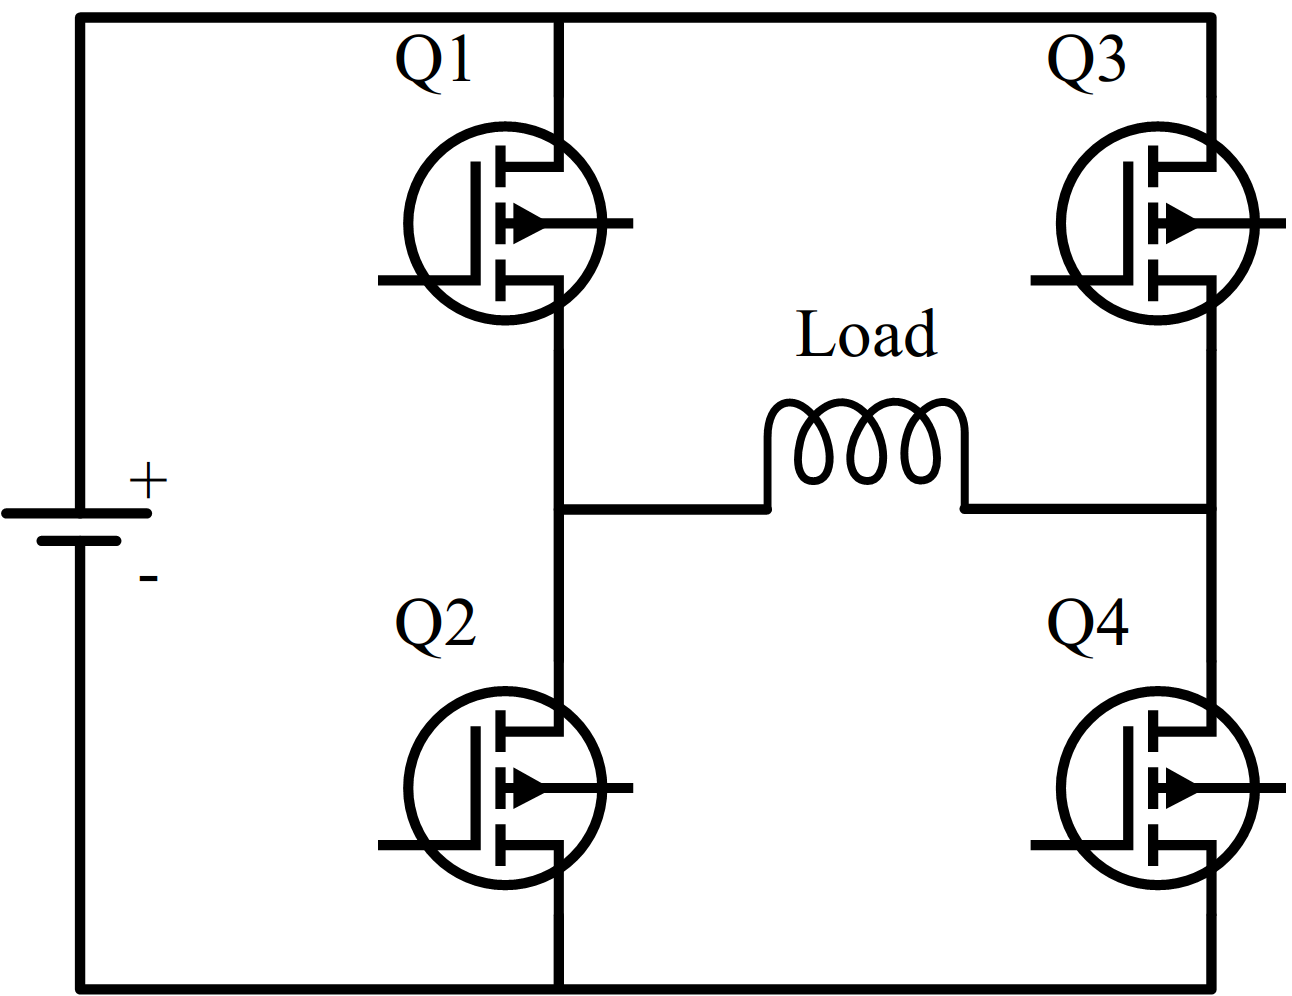
\includegraphics[scale=1.0]{5-amplifier.png}
	\caption{开关功率放大器单路全桥拓扑}
	\label{fig:5-amplifier}
\end{figure}


4.控制板卡

控制板卡包含一块STM32F407芯片和一块Cyclone IV EP4CE40芯片,以及信号调理电路、驱动隔离电路等外围电路。

STM32F4系列单片机是意法半导体公司(ST)推出的基于ARM Cortex-M4内核的高性能微控制器,搭载NVM技术和ART加速器技术,使得该系列单片机的计算性能可达225DMIPS(主频运行于180MHz)。此外,其集成的单周期DSP指令和浮点运算单元(FPU,Floating Point Unit),具备高效完成复杂数学浮点运算的能力。本文使用的STM32F407ZET6参数如\autoref{tab:stm32_para}所示。

\begin{table}[htb]
  \caption[STM32F407ZET6性能参数]{STM32F407ZET6性能参数\label{tab:stm32_para}}
  \begin{tabular}{cc}
    \toprule
    模块 & 性能值 \\
    \midrule
    Flash & 512KB\\
    RAM & 192KB\\
    定时器 & 12$\times$ 16-bit + 2$\times$ 32-bit\\
    ADC & 24 $\times$ 12-bit\\
    DAC & 2 $\times$ 12-bit\\
    USART + UART & 4 + 2\\
    Ethernet & 1	\\
    \bottomrule
  \end{tabular}
\end{table}

Cyclone IV E系列芯片是Intel公司2009年推出的低成本、低功耗、较高性能的FPGA芯片解决方案。Cyclone IV E系列基于优化的60纳米低功耗制程技术构建,配备逻辑单元、片上存储单元、片上乘法器、锁相环(PLL)、全局时钟网络以及数量众多的普通I/O端口。本文选用的是Cyclone IV EP4CE40F23I7,其主要参数如\autoref{tab:fpga_para}所示。

\begin{table}[htb]
  \caption[Cyclone IV EP4CE40F23I7性能参数]{Cyclone IV EP4CE40F23I7性能参数\label{tab:fpga_para}}
  \begin{tabular}{cc}
    \toprule
    模块 & 性能值 \\
    \midrule
    逻辑单元 & 39600\\
    嵌入式存储 & 1134KB\\
    嵌入式18$\times$18乘法器 & 116\\
    通用型PLL & 4\\
    全局时钟网络 & 20\\
    用户I/O组 & 8\\
    最大用户I/O & 532	\\
    \bottomrule
  \end{tabular}
\end{table}

\section{软件设计}
磁悬浮轴承控制系统软件部分的实现基于前文所述的硬件组件和板载电路,软件控制目标是使转子在高速旋转时,仍稳定悬浮在磁悬浮轴承中心,且具备抗干扰和抗冲击能力。为实现该目标,本文搭建了一套由上位机程序、STM32单片机程序和FPGA程序共同组成的磁悬浮轴承控制软件。顶层软件结构如\autoref{fig:5-software_top}所示。FPGA拥有高速并行计算能力,因此磁轴承闭环控制中的外环和内环控制均部署于其中计算。为防止系统意外故障致转子跌落损伤轴承,FPGA实时监控转子位移波形,在检测到异常发生时自动切断电机驱动器。借助于STM32F4系列的丰富通讯接口,其承担“数据中转站”的功能——采集FPGA中的控制状态量然后传输给PC,或接收PC指令然后写入到FPGA控制寄存器中。此外,STM32F4采集和监测电机和轴承温度,保证系统工作温度正常。PC上运行基于Matlab/Appdesigner模块设计的上位机程序,用于读写FPGA控制状态量以及进行数据采集与分析。
\begin{figure}
	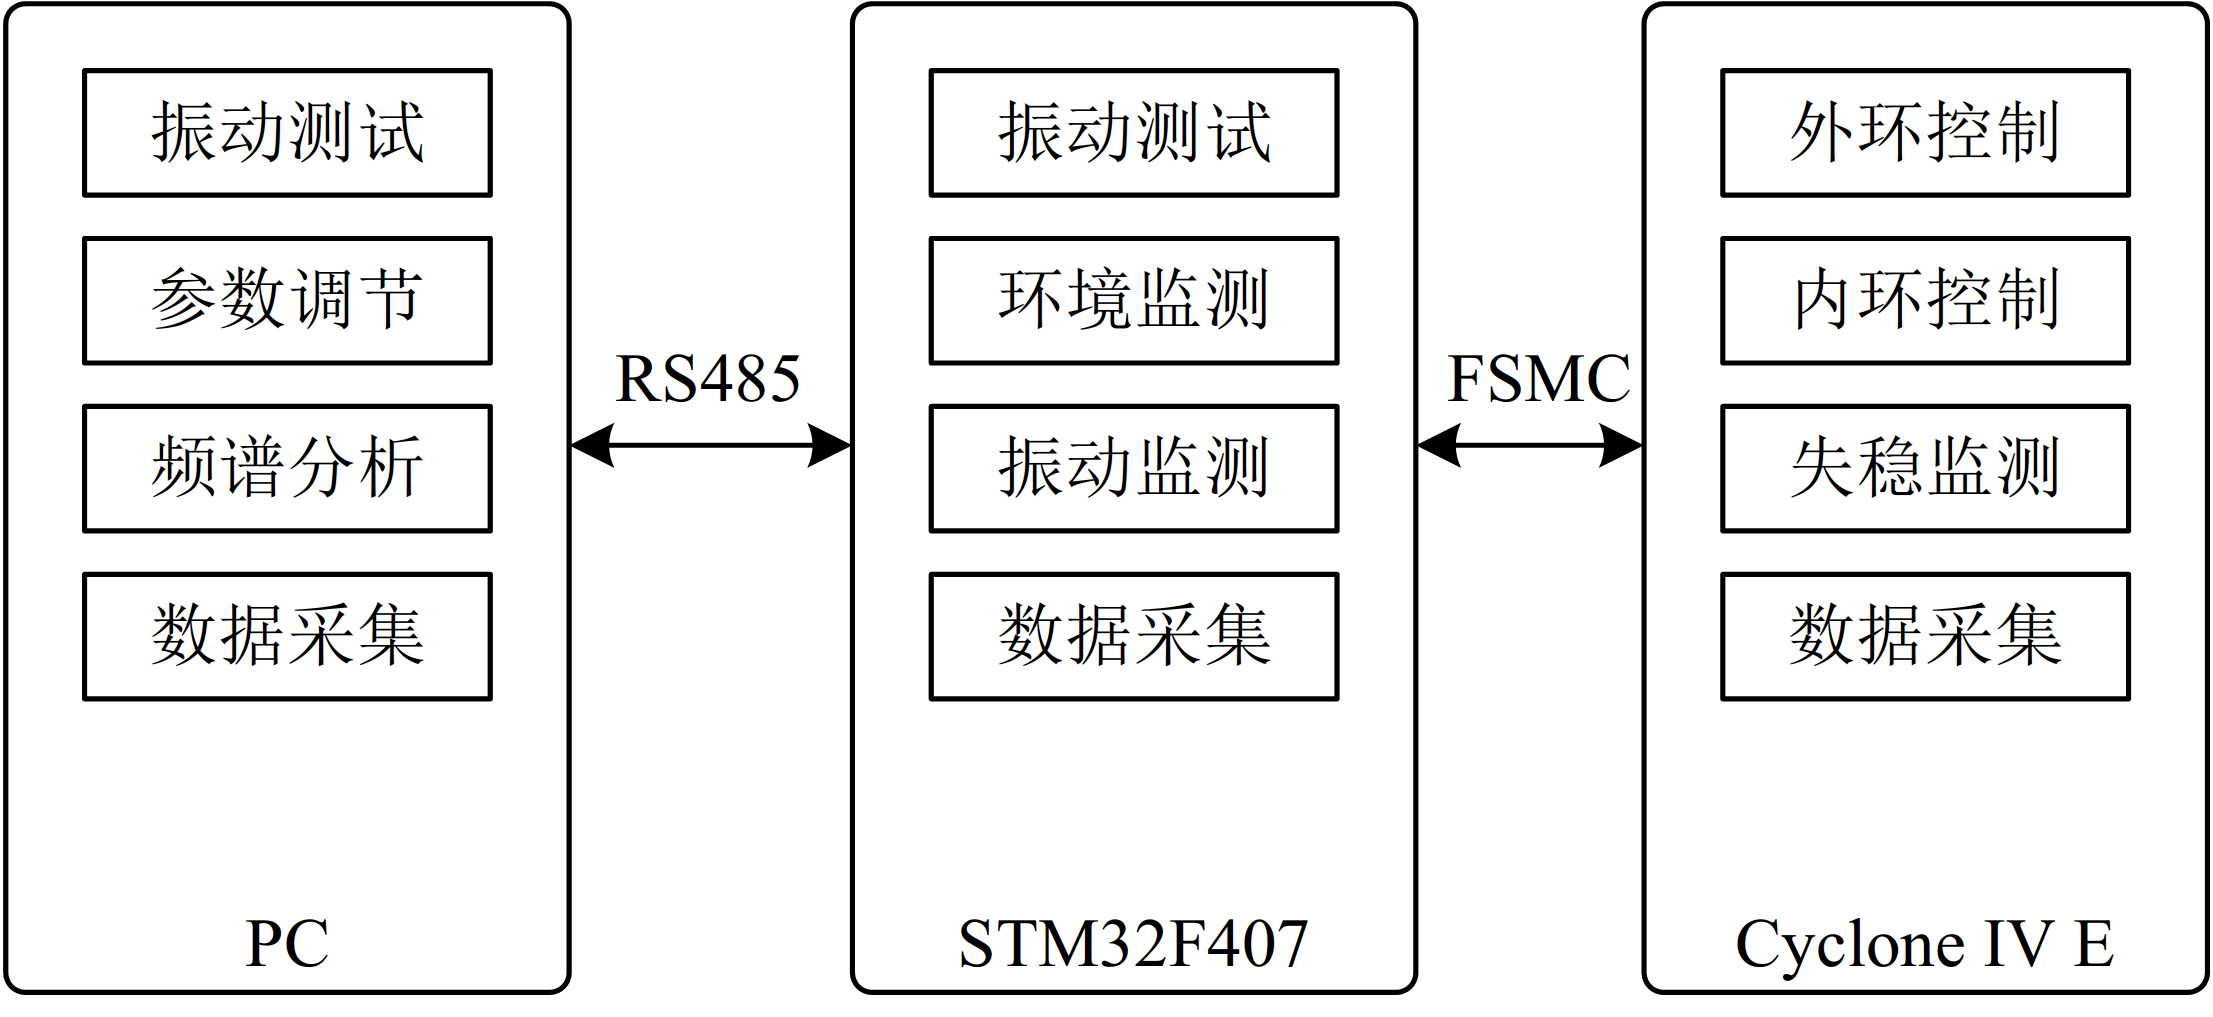
\includegraphics[scale=1.0]{5-software_top.png}
	\caption{磁轴承系统控制顶层软件结构}
	\label{fig:5-software_top}
\end{figure}

\subsection{实时控制程序}
实时控制程序是控制磁悬浮轴承的核心程序,包括内环控制和外环控制,如\autoref{fig:5-software_rtcontrol}所示。其中外环是指转子位移控制:位移传感器采集转子位置,外环控制器目标是使转子实际位置跟踪人为给定位置。内环是指磁悬浮轴承线圈电流控制:磁悬浮轴承通过线圈电流激发磁场,进而产生磁悬浮力控制转子位置,内环控制器目标是使线圈实际电流跟踪外环控制器输出给定电流。

\begin{figure}
	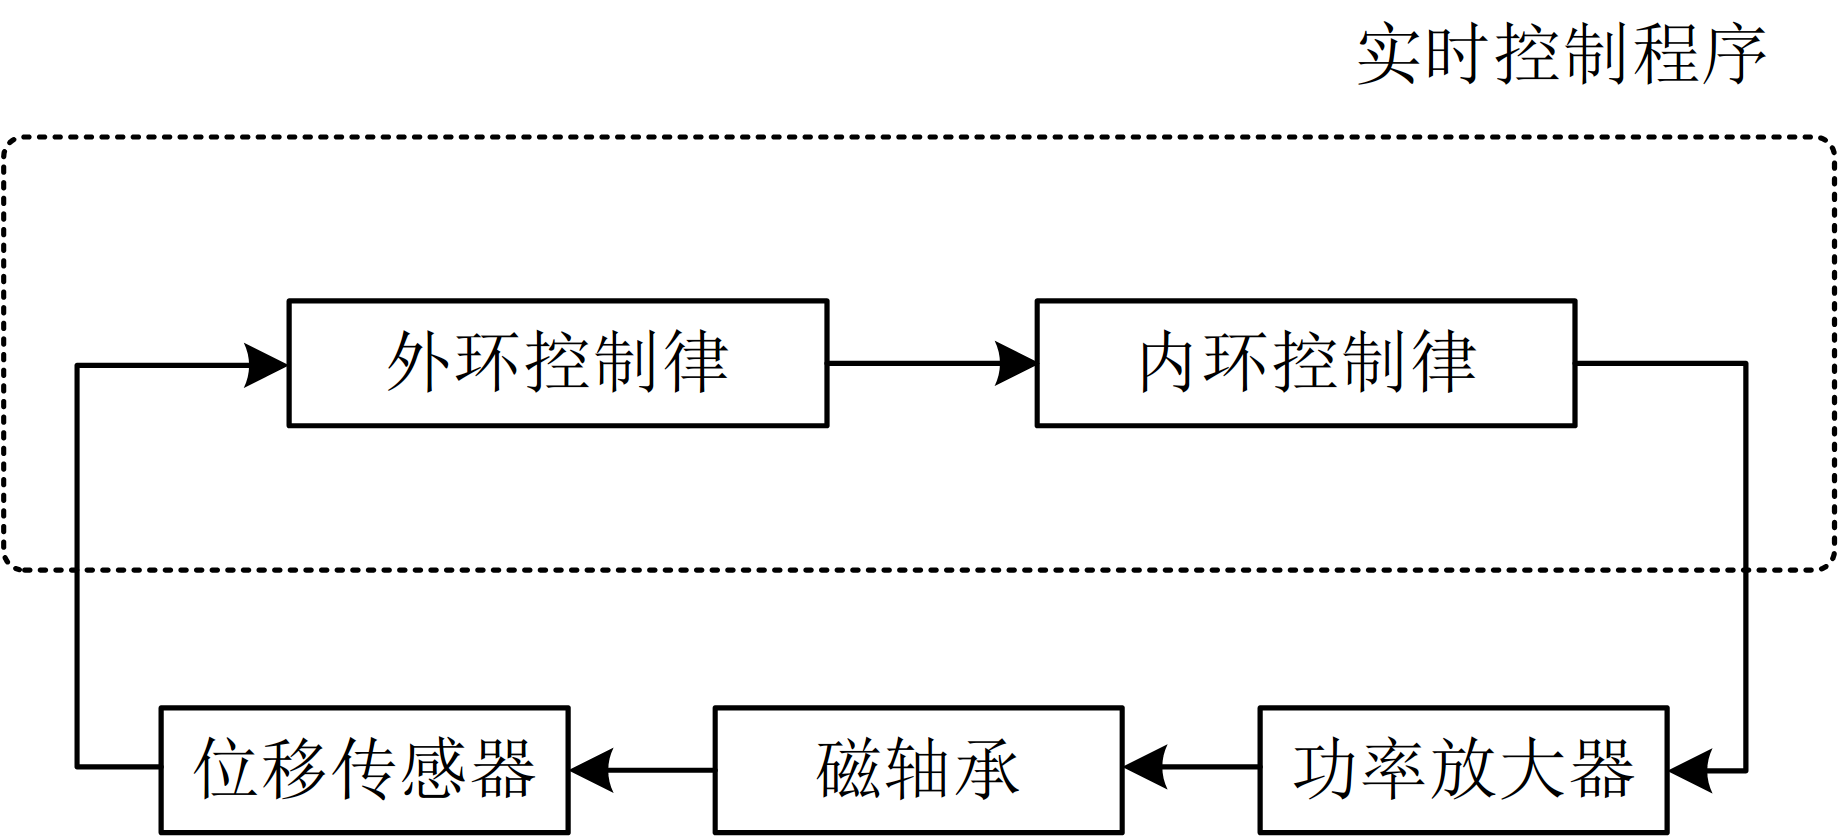
\includegraphics[scale=1.0]{5-software_rtcontrol.png}
	\caption{磁轴承系统实时控制程序}
	\label{fig:5-software_rtcontrol}
\end{figure}

\subsection{用户交互程序}
用户交互程序包括参数调节程序和灵敏度函数测试程序。

外环控制器和内环控制器的参数需要根据系统仿真设计值进行初步设计,然而现场根据磁悬浮电机运行状况进行进一步细致调节。磁悬浮轴承双环控制器参数多(约四十个可调参数),且通常需要连续调节以观察转子控制效果。传统参数调节方式有在程序内常量方式写入到Flash中,但该方法不适合需要频繁修改参数的场景;另一种常规方法是通过编程软件中的变量观察窗口进行参数手动输入。显然,这两种传统参数调节方式无法满足本文设计的双环控制器参数调节需求。因此本文开发桌面版参数调节程序来完成参数调节任务。

参数调节程序如\autoref{fig:5-software_para}所示。使用该程序可以单独调节每一自由度的控制参数,也可以联动调节磁悬浮轴承单端的两个自由度参数。外环和内环的每一个参数的调节范围可任意设置,通过拖动滚动条实现该参数连续变化调节。该软件使用步骤为:控制板卡上电后,启动该软件。依次点击各个自由度的【Pull】按钮读取该自由度参数的当前值。手动设置各个参数的范围,拖拉滚动条即可将新的参数值写入到控制板卡上。完成参数调节后,退出软件。

\begin{figure}
	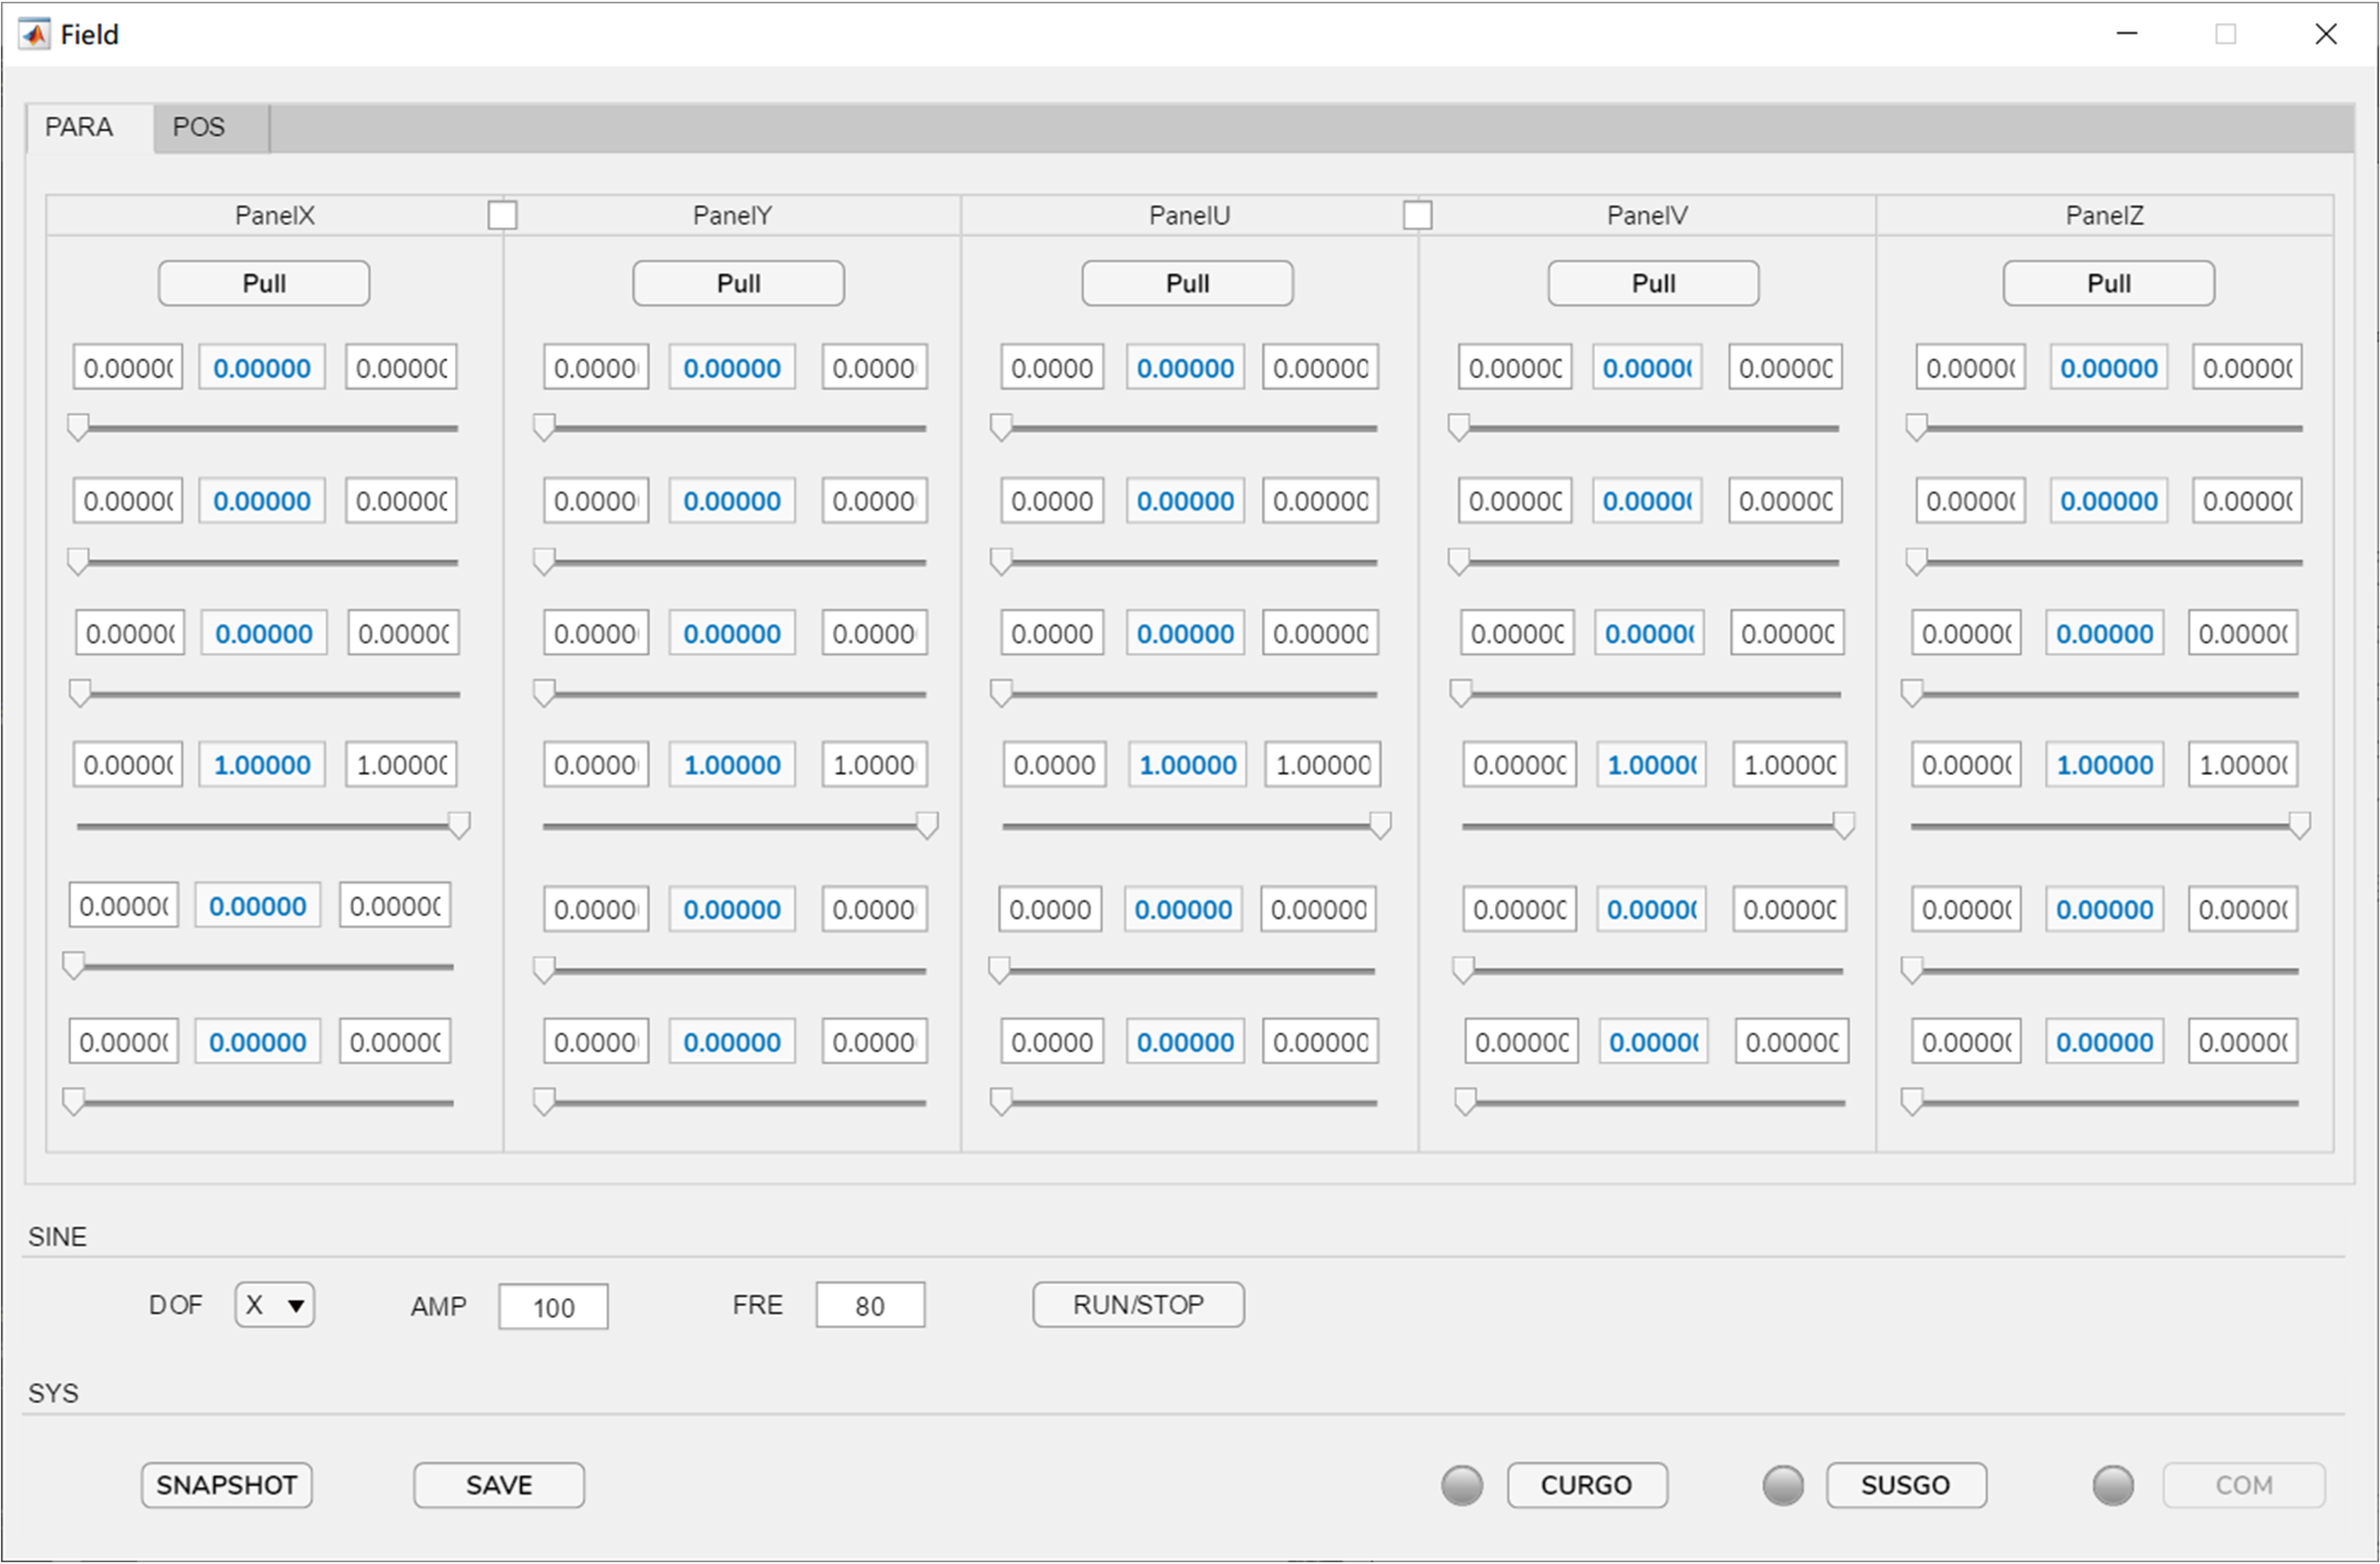
\includegraphics[scale=1.0]{5-software_para.png}
	\caption{磁轴承系统参数调节程序}
	\label{fig:5-software_para}
\end{figure}

灵敏度函数测量程序用于测试各个自由度的灵敏度函数,其原理是在给定位移信号上叠加一定幅值和一定频率的正弦信号用作激励,采集反馈位移信号的幅值和相位当做响应,通过测量激励信号和响应信号在一定频率区间上的增益衰减和相位偏差,可以得到该自由度的频率响应特性,即灵敏度函数。

灵敏度函数测量程序如\autoref{fig:5-software_sen.png}所示。该程序可以设置激励信号的幅值和频率、设置激励信号频率扫描范围,测量过程实时显示前序频率点的测量结果。该软件使用步骤为:控制板上电后,运行该程序,点击【SUSGO】按钮启动转子悬浮。依次设置测量自由度、激励信号幅值、扫描频率范围后,点击【Start】按钮。程序开始运行测量程序。测量过程中,列表会显示前序扫描频率点和扫描结果,图框中显示频率-幅值曲线和频率-相位曲线。所有频率扫描完成后,可以选择继续测量下一通道。如完成测量,即可退出软件。

\begin{figure}
	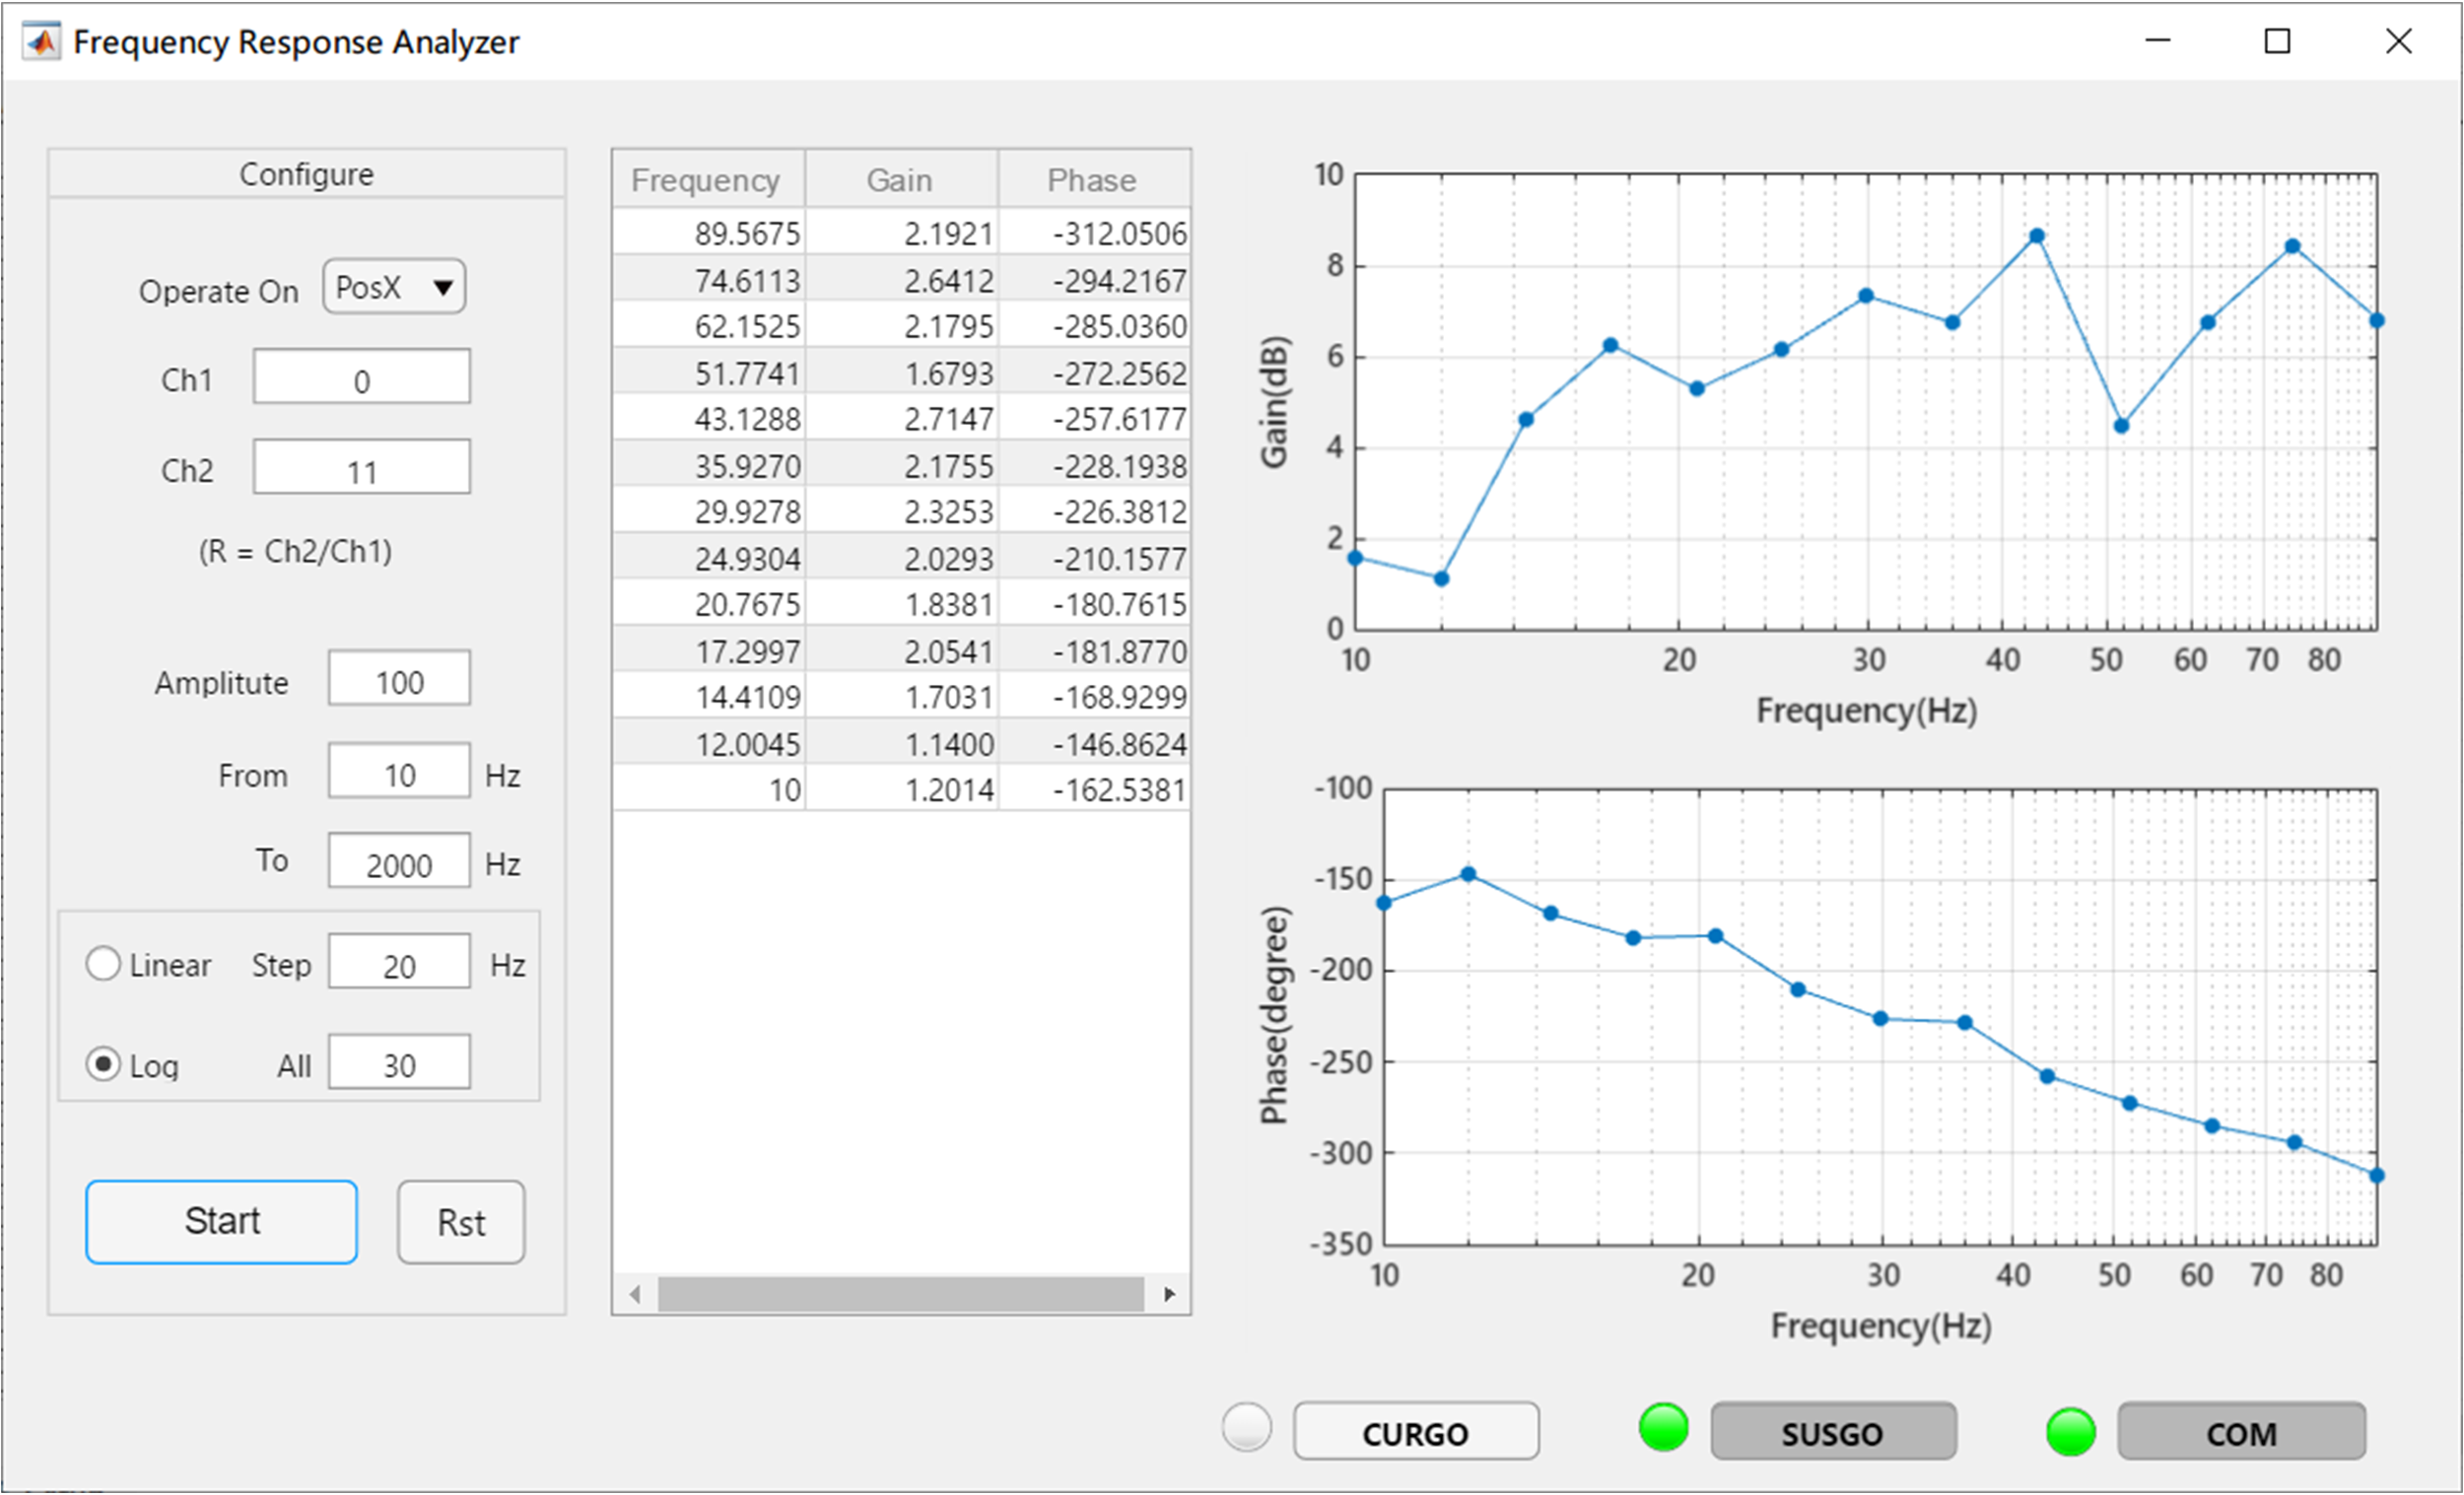
\includegraphics[scale=1.0]{5-software_sen.png}
	\caption{磁轴承系统灵敏度函数测量程序}
	\label{fig:5-software_sen}
\end{figure}

\section{磁悬浮轴承输出敏感度测定实验}
磁悬浮轴承的轴承刚度和轴承阻尼均可以通过主动控制的方式来调节,然而作为传统机械轴承的替代品,其最应该具备的基本性能是保持稳定,即要求磁悬浮轴承在严苛工况下也能保持支撑转子的能力。数字控制系统中,依据传递函数计算系统特征根位置是主要的系统稳定性分析方法。但是只有获取到准确的参数值,如位移刚度和电流刚度时,根据传递函数解算出的系统特征根才比较准确。实际上理论模型和实际模型很难一致,这是因为电机与轴承加工和装配、位移传感器等系统组件总是会引入存在一定的误差。因此,我们需要找到一种便于实际应用且能准确表征系统稳定性能的方法。

磁悬浮轴承ISO 14839-3标准\cite{iso2004mechanical}定义了输出敏感度函数,用于定量分析磁悬浮轴承的稳定性能。定义输出敏感度函数为$S_0$,显示在\autoref{fig:5-sen}中:
\begin{equation}
	S_0 = \frac{V_2}{V_1}
\end{equation}
其中$G_p$表示磁悬浮轴承本体的传递函数,$G_c$表示控制器的传递函数。注意到
\begin{figure}
	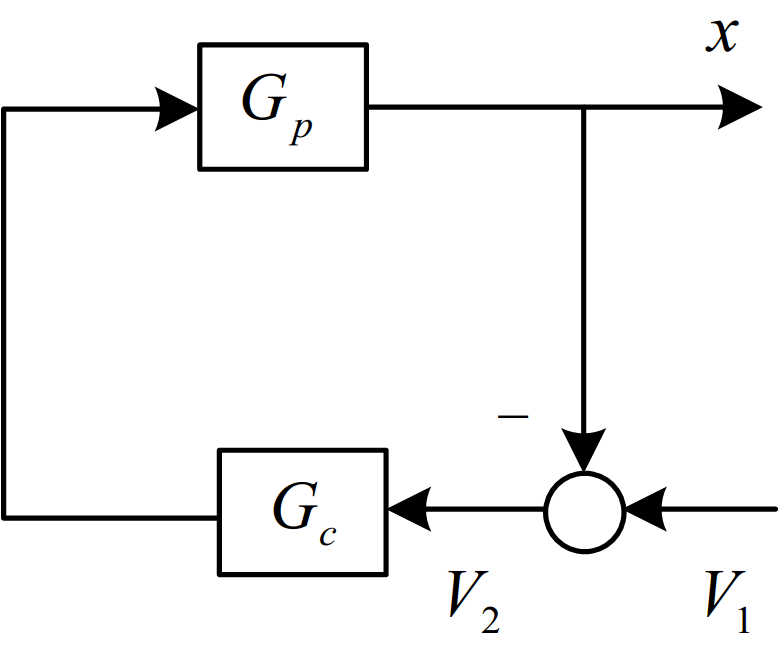
\includegraphics[scale=1.0]{5-sen.png}
	\caption{磁悬浮轴承输出敏感度示意图}
	\label{fig:5-sen}
\end{figure}

\begin{equation}
	S_0(j\omega) = \frac{1}{1 + G_p(j\omega)G_c(j\omega)}
\end{equation}
$1 + G_p(j\omega)G_c(j\omega)$的值越大,则奈奎斯特图上$G_p(j\omega)G_c(j\omega)$与点$(-1,0)$的距离越远,增益裕度越大。那么我们可以通过敏感度函数$S_0(j\omega)$来判定系统增益裕度:敏感度函数$S_0(j\omega)$的峰值越小,增益裕度越大。

敏感度函数测试频率上限通常没有定值,因为敏感度函数超过一定的频率之后,其幅值趋近于1。即随着在敏感度函数测试点注入的激励信号的频率升高,响应点检测的信号幅值会趋近于激励信号本身的幅值。ISO 14839-3标准规定了敏感度函数测试频率的上限为转子额定频率的三倍,但若该值超过2kHz,则取上限为2kHz。

通常磁悬浮轴承控制是采用分散的五自由度独立控制,测试方法为依次在各个通道的测试点上注入激励信号,检测响应信号,得到一个通道的敏感度函数。该过程中其它通道须保持闭环控制。

经上述过程测量得到的敏感度函数测量结果可以表示为:
\begin{equation}
	S_{0,max} = max \left[ max_i \left|G_s(j\omega)\right| \right]
\end{equation}
其中频率范围为$\omega = 2 \pi f$,$0 \leq f \leq 2kHz$;测量通道序号为$i$,分别指需要测量的五个自由度。系统的全局稳定性能优劣取决于敏感度函数峰值最大的一个通道。

对于输出敏感度测量结果,ISO 14839-3定义了稳定区间标准如下:

\begin{table}[htb]
  \caption[ISO 14839-3定义磁悬浮轴承输出敏感度函数峰值稳定区间标准]{ISO 14839-3定义磁悬浮轴承输出敏感度函数峰值稳定区间标准\label{tab:amb_iso}}
  \begin{tabular}{cc}
    \toprule
    输出敏感度函数峰值 & 稳定区间 \\
    \midrule
    $(-\infty,9.5dB]$ & A\\
    $(9.5dB,12dB]$    & B\\
    $(12dB,14dB]$     & C\\
    $(14dB,\infty)$   & D\\
    \bottomrule
  \end{tabular}
\end{table}

新出厂的商用磁悬浮轴承的输出敏感度峰值应落在A区间;对于非严格的使用环境,落在B区间也是可以接受的;对于输出敏感度函数峰值落在C区间的磁悬浮轴承,通常不宜长期运行;若输出敏感度函数峰值落在D区间,则表明该磁悬浮轴承应立即检修。
\begin{figure}
	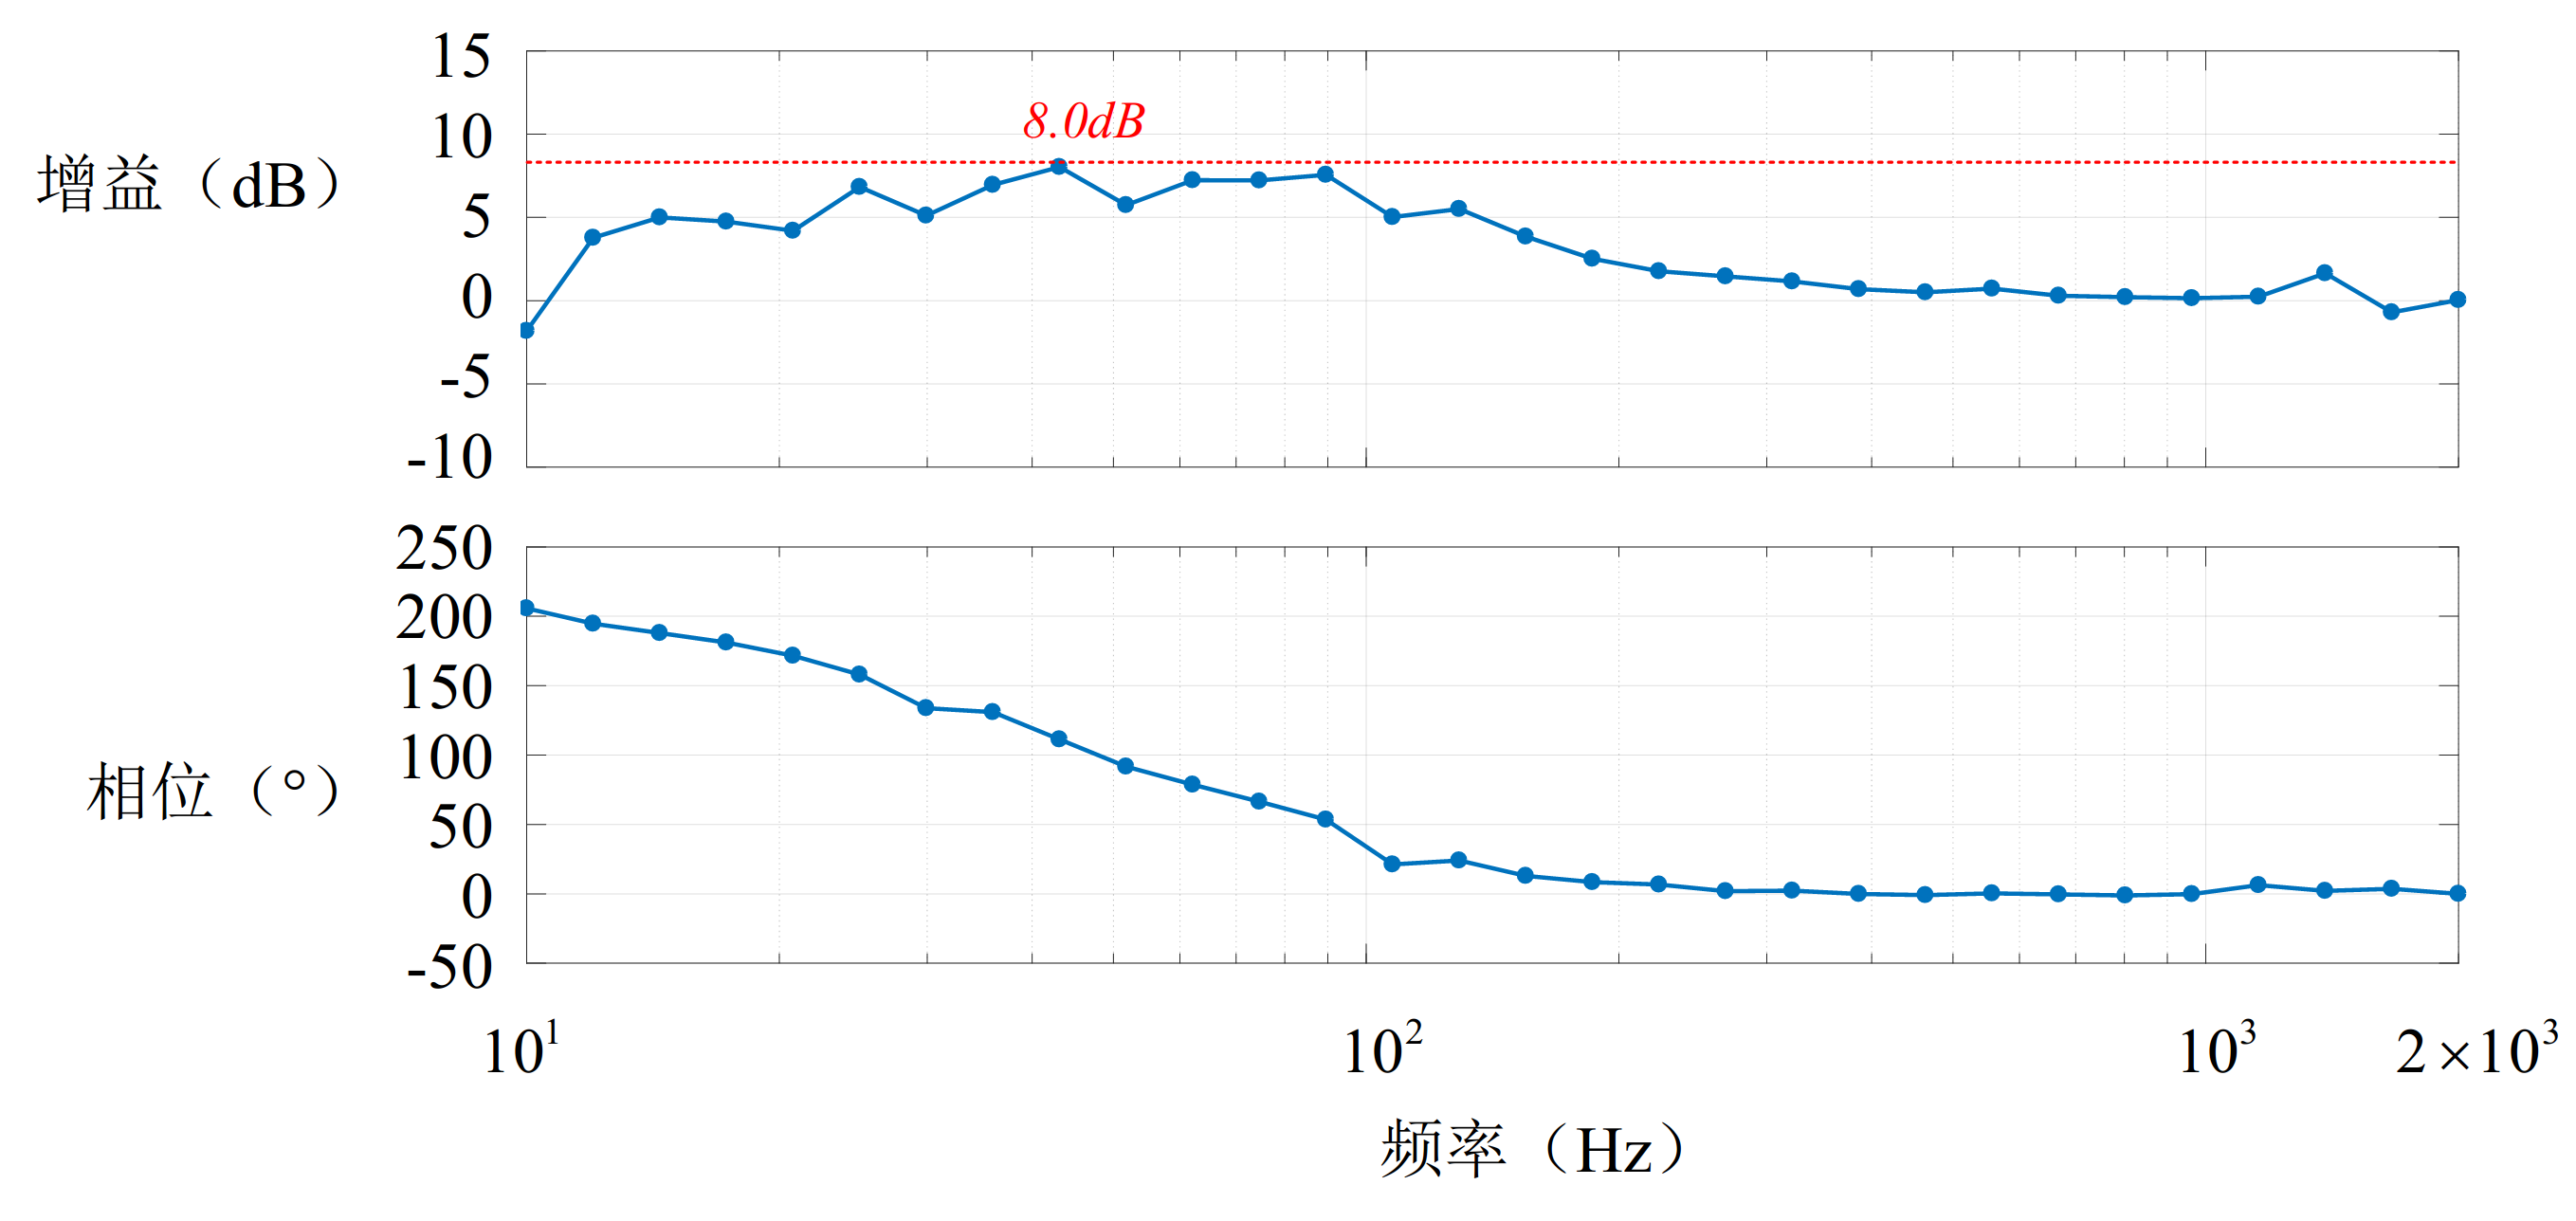
\includegraphics[scale=1.0]{5-sens_x.png}
	\caption{B端水平方向控制通道输出敏感度函数曲线}
	\label{fig:5-sens_x}
\end{figure}

\begin{figure}
	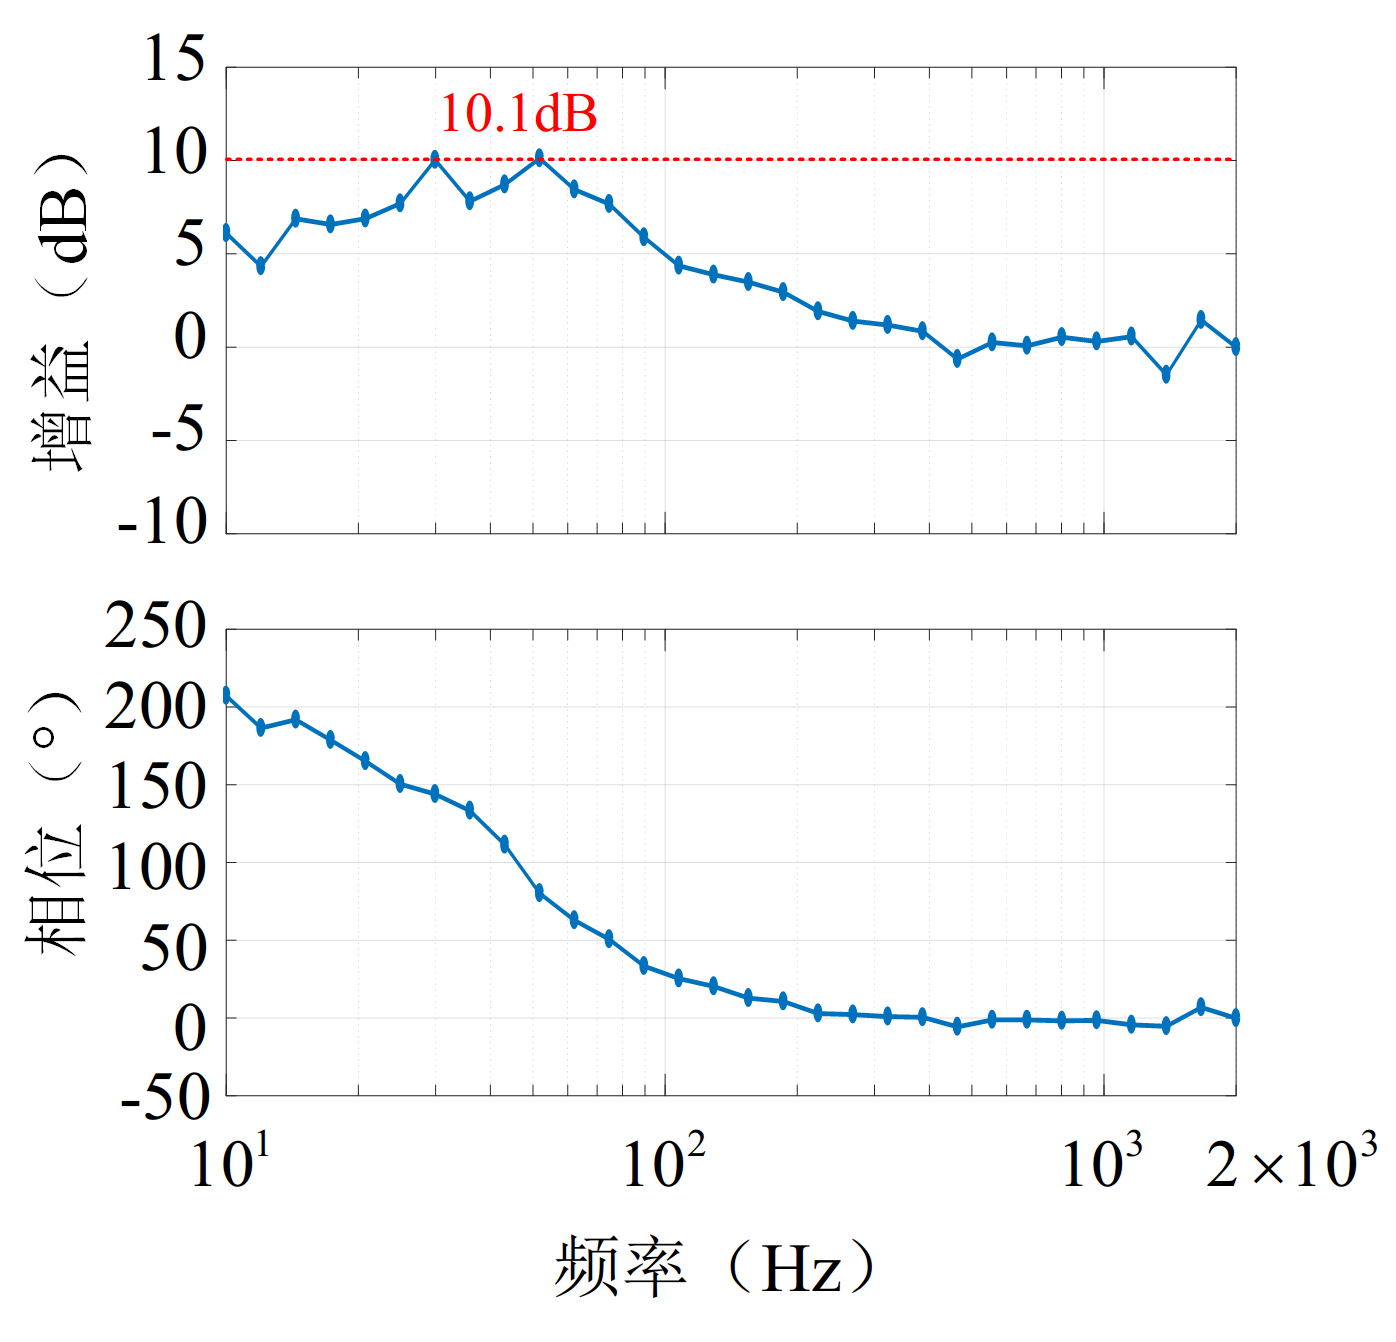
\includegraphics[scale=1.0]{5-sens_y.png}
	\caption{B端竖直方向控制通道输出敏感度函数曲线}
	\label{fig:5-sens_y}
\end{figure}

\begin{figure}
	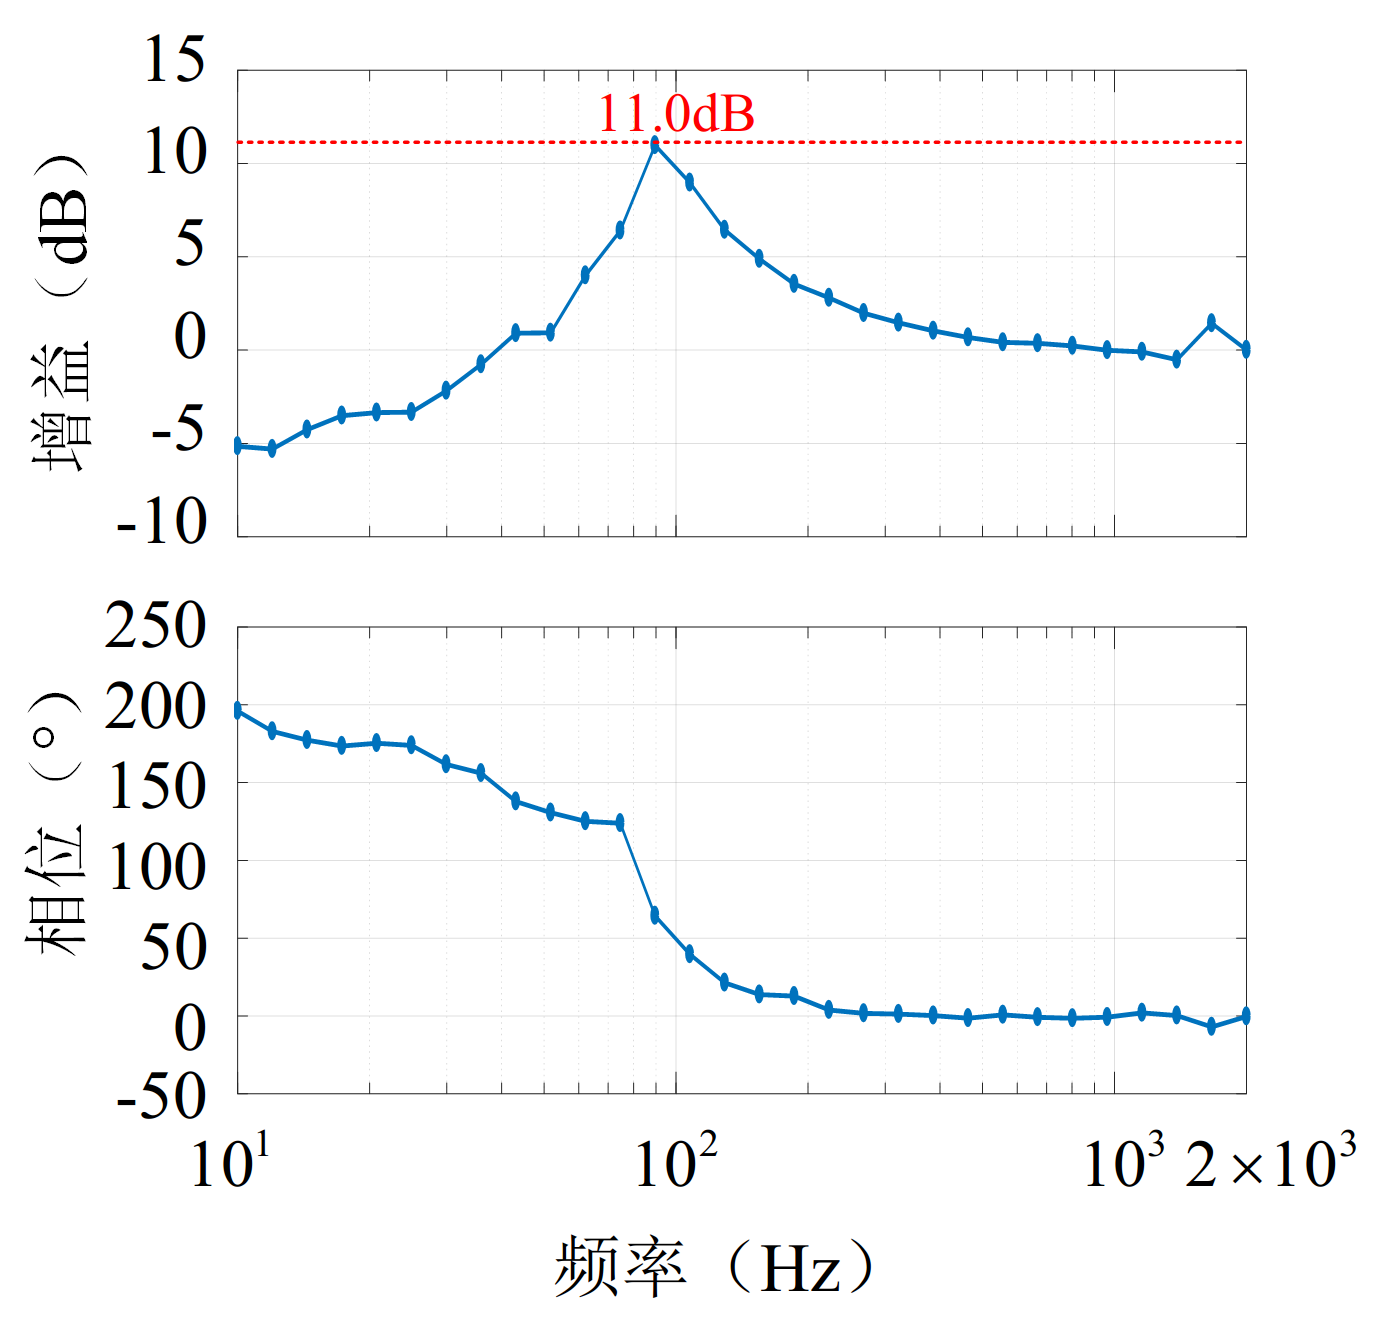
\includegraphics[scale=1.0]{5-sens_u.png}
	\caption{A端水平方向控制通道输出敏感度函数曲线}
	\label{fig:5-sens_u}
\end{figure}

\begin{figure}
	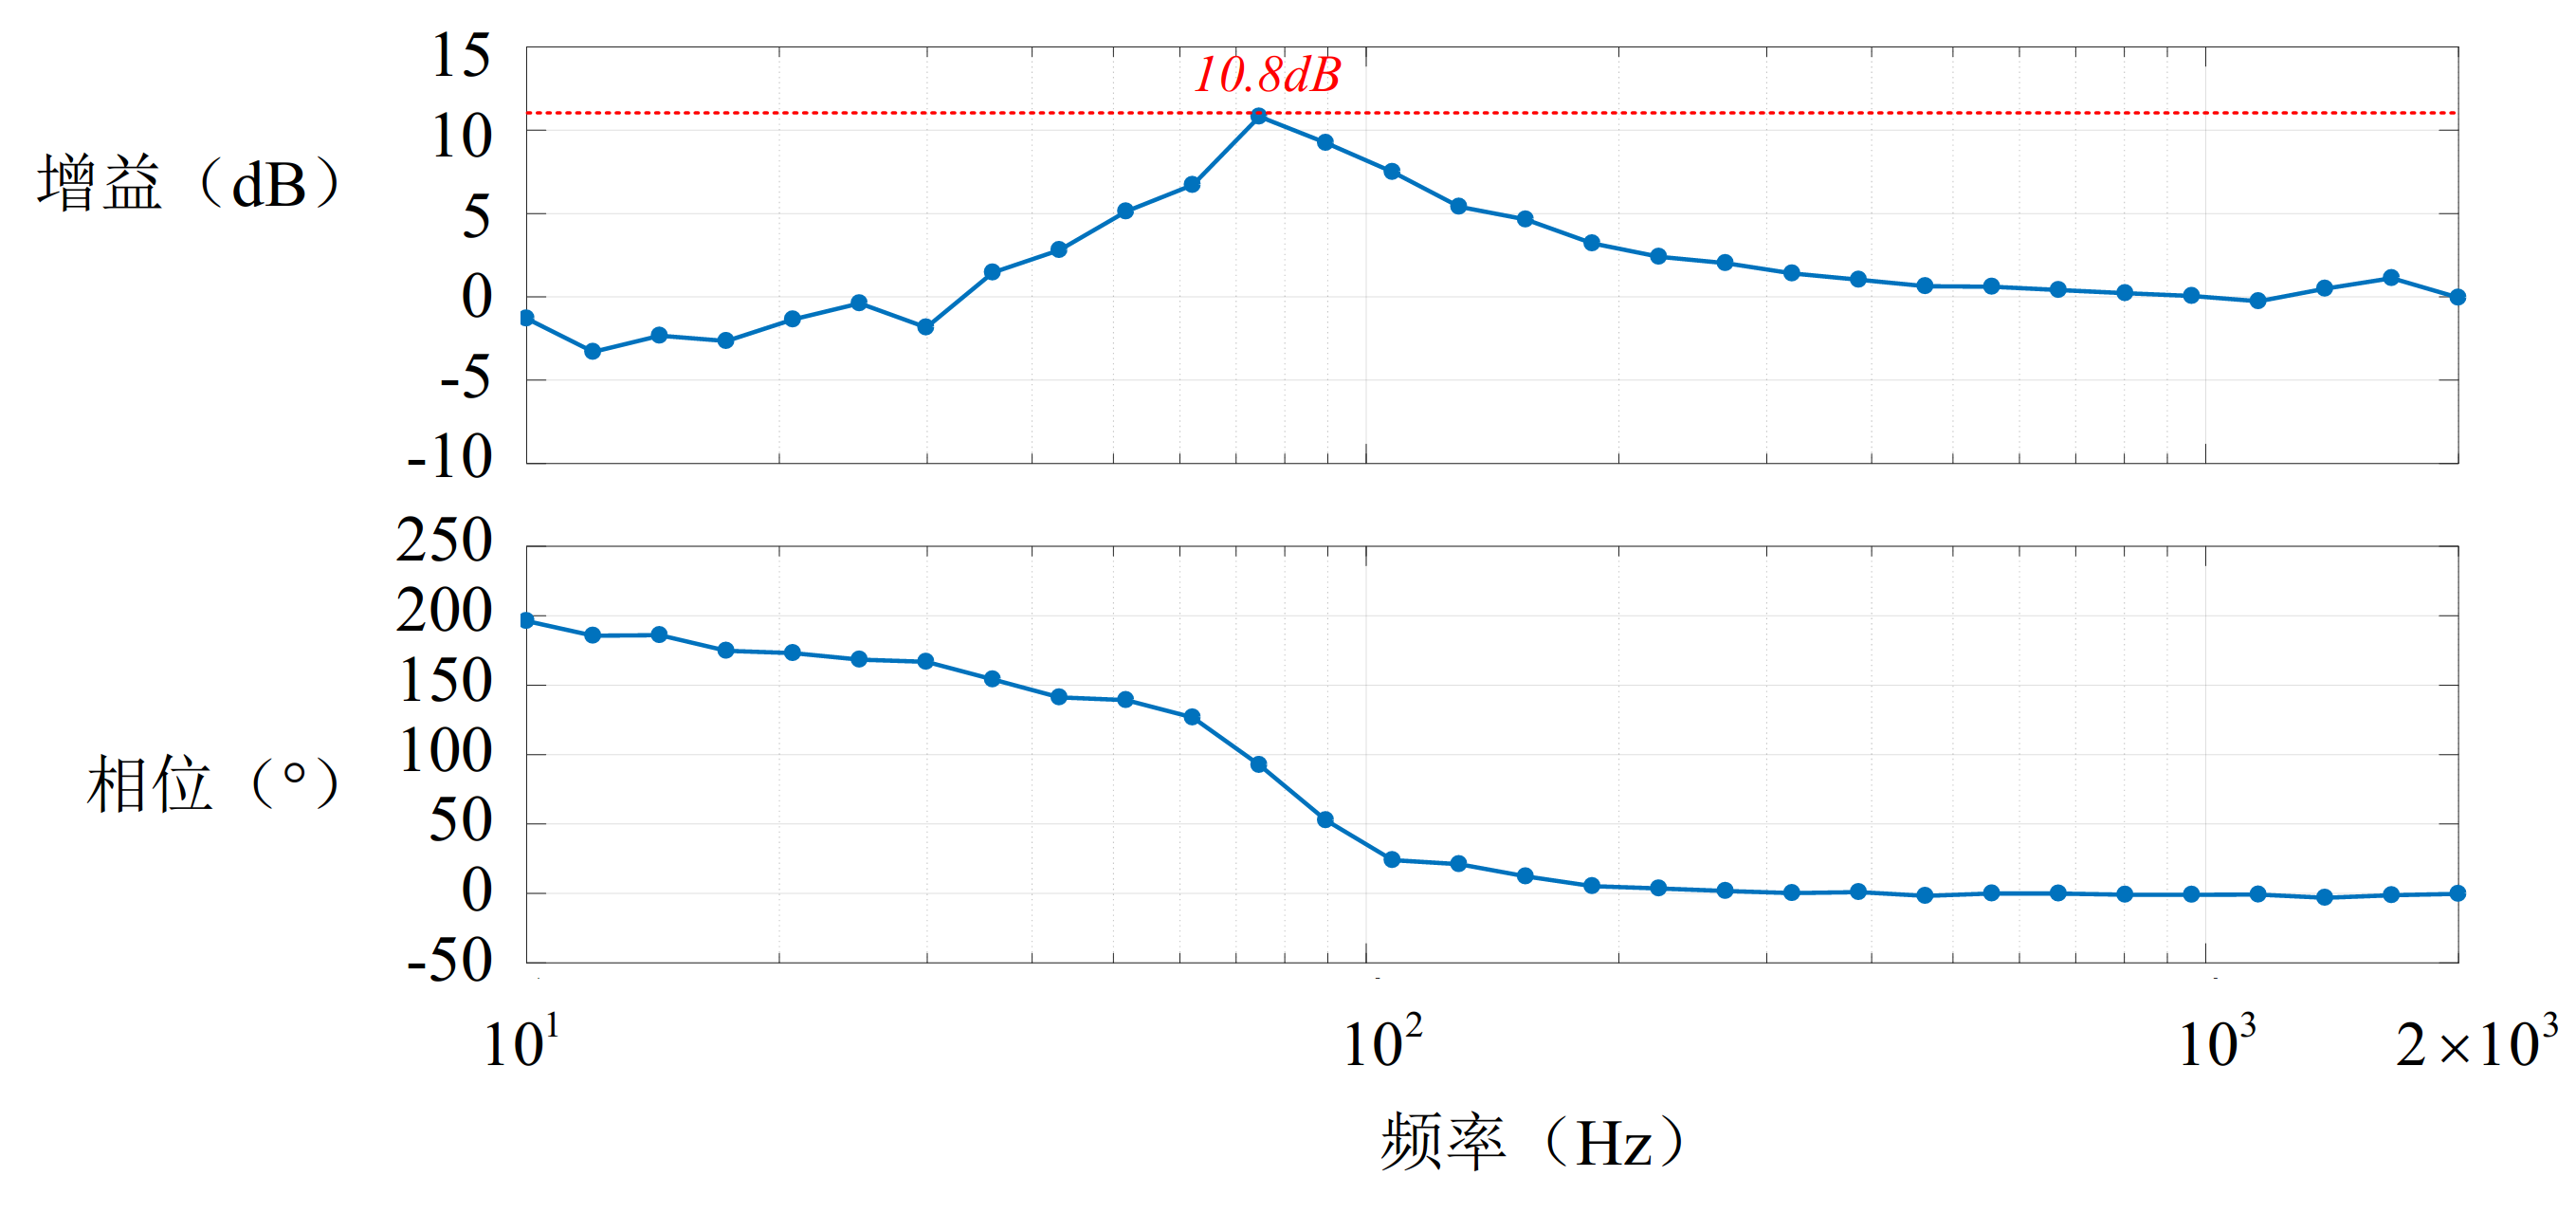
\includegraphics[scale=1.0]{5-sens_v.png}
	\caption{A端竖直方向控制通道输出敏感度函数曲线}
	\label{fig:5-sens_v}
\end{figure}

\begin{figure}
	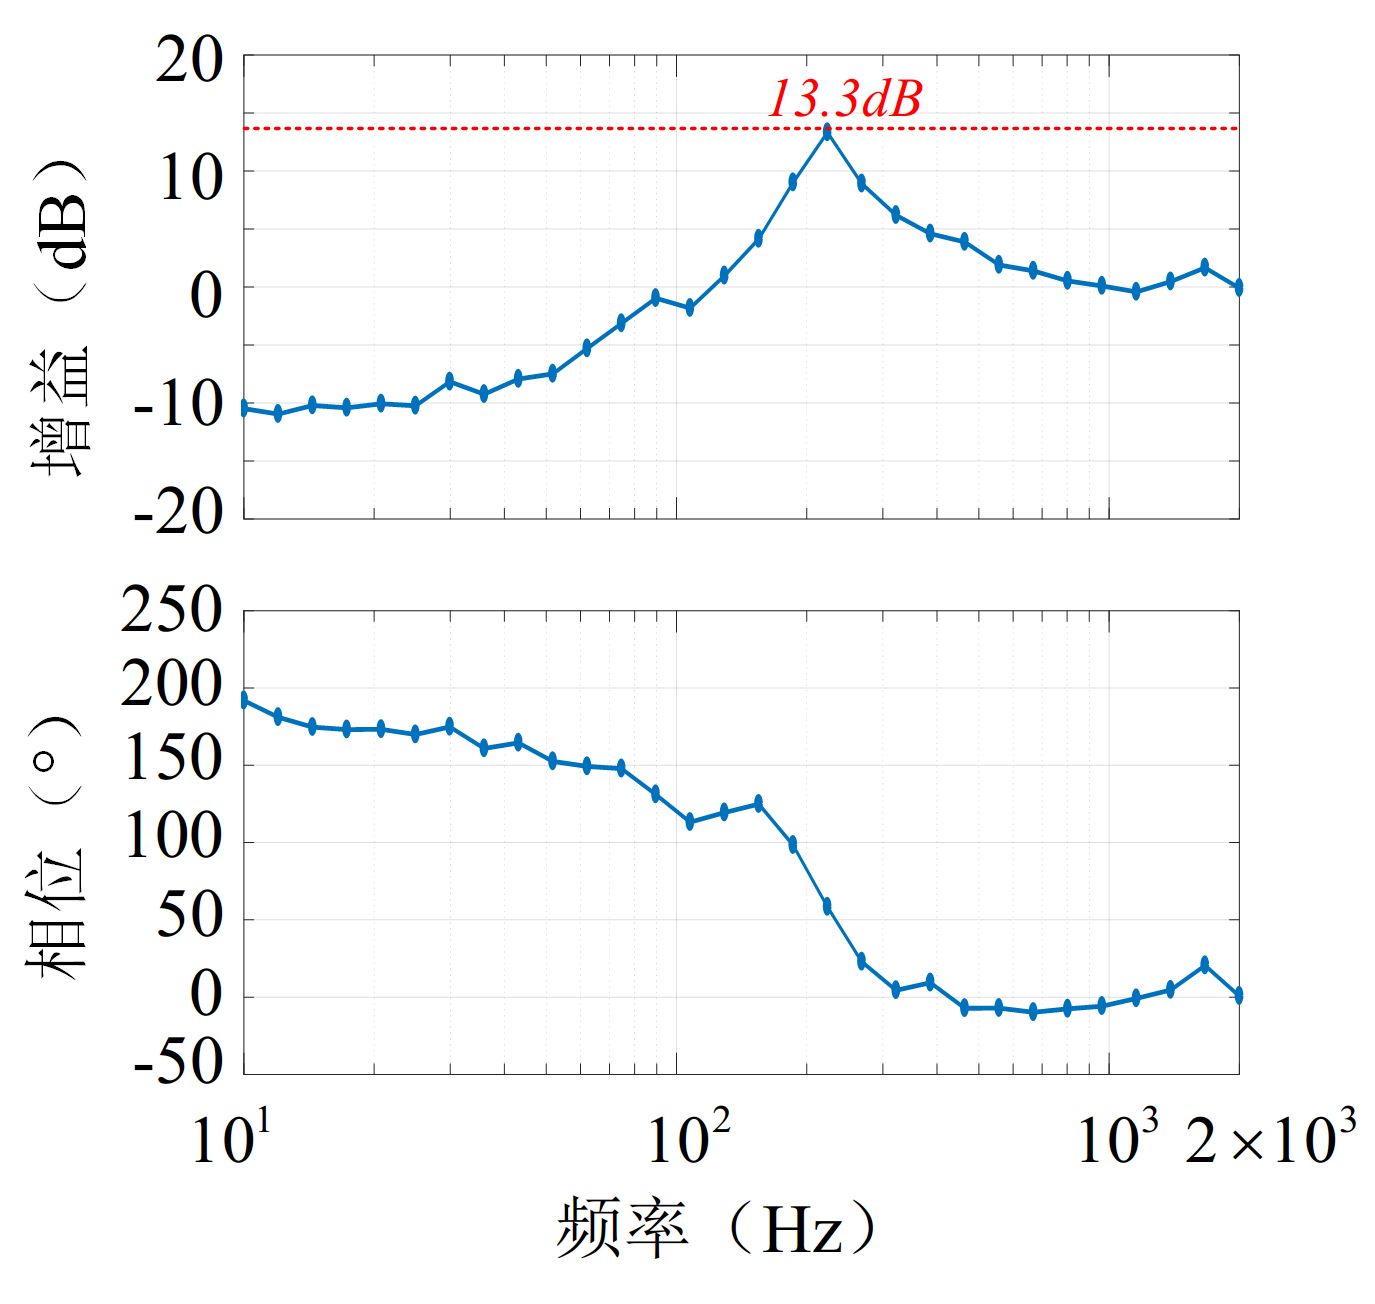
\includegraphics[scale=1.0]{5-sens_z.png}
	\caption{轴向控制通道输出敏感度函数曲线}
	\label{fig:5-sens_z}
\end{figure}

从\autoref{fig:5-sens_x}~\autoref{fig:5-sens_z}所示的输出敏感度测量结果可以看出,四个径向自由度的输出敏感度函数的峰值分别为8.0dB、10.1dB、11.0dB和10.8dB,轴向自由度的输出敏感度函数的峰值为13.3dB。其中径向自由度的输出敏感度峰值均落在B区间,轴向自由度的输出敏感度峰值落在C区间。按照ISO标准,该实验样机满足短期运转的实验测试需求。


\section{基于奇数次零相移重复控制器的在线振动抑制实验}
第三章中对比了传统整数次重复控制器和奇数次零相移重复控制器的原理,仿真结果显示零相移奇数次重复控制器能更有效的抑制磁悬浮轴承控制电流中的谐波分量。本小节在样机上进行实验,验证传统整数次重复控制器和奇数次零相移重复控制器的原理。

\begin{figure}
	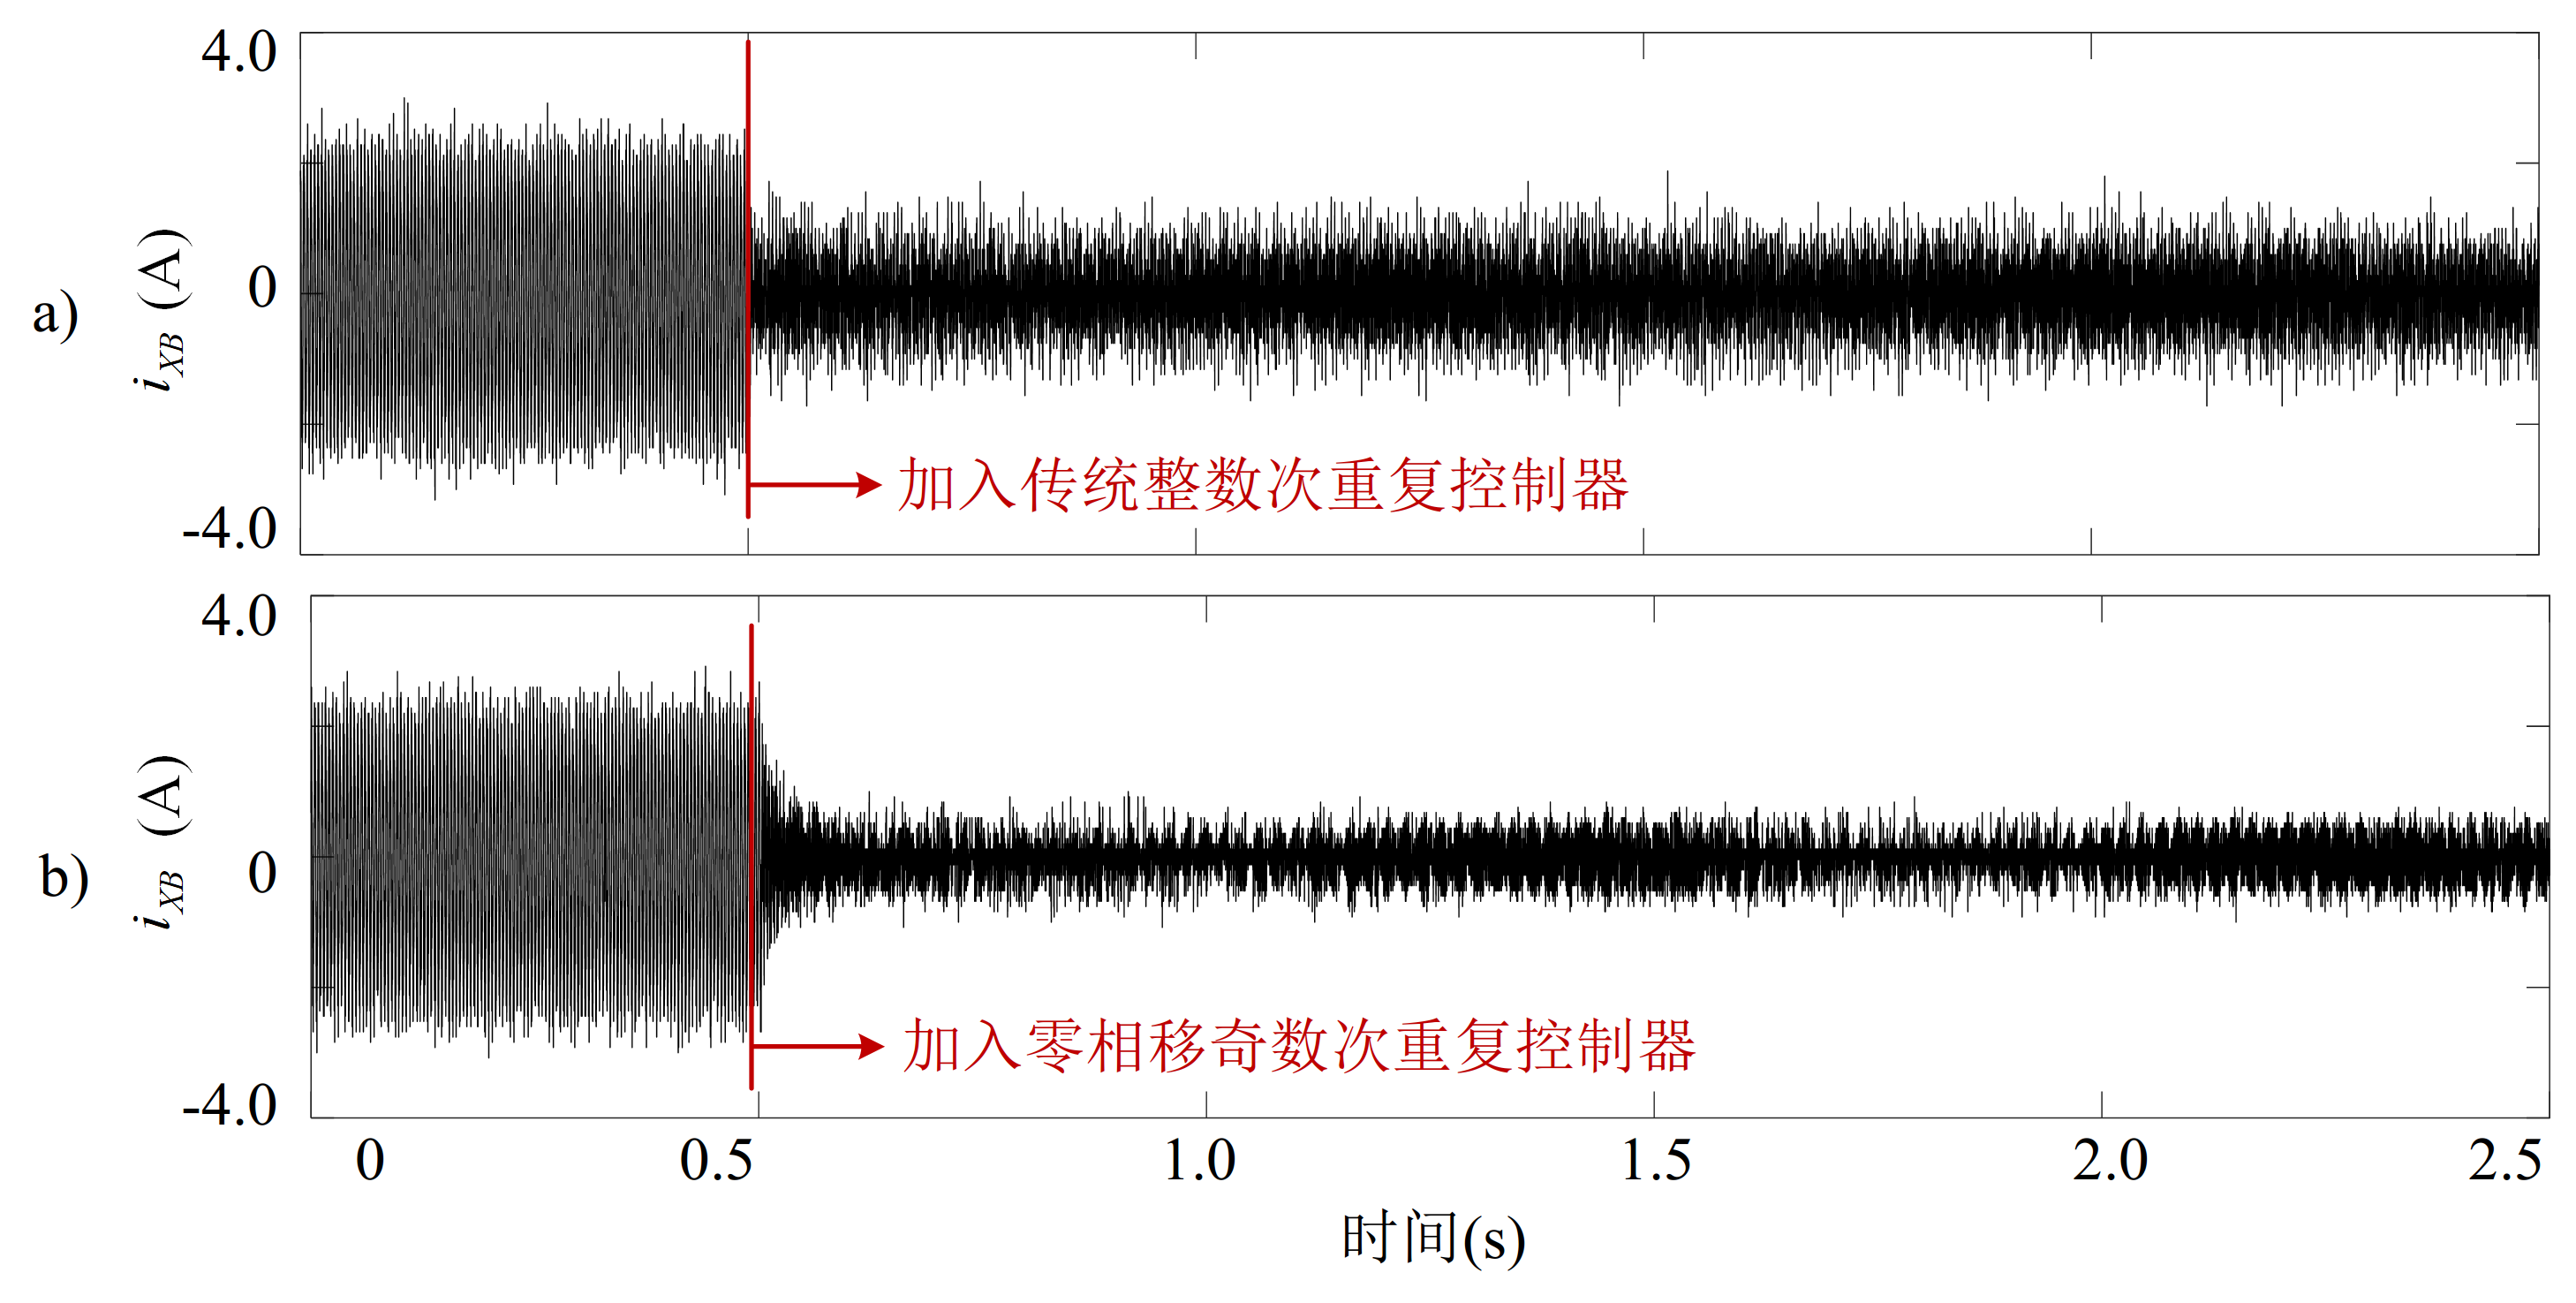
\includegraphics[scale=1.0]{5-orc_current.png}
	\caption{转子250Hz时的线圈电流时域波形实验测量结果,a)加入传统重复控制器前后电流波形,b)加入奇数次零相移重复控制器前后电流波形}
	\label{fig:5-orc_current}
\end{figure}

\autoref{fig:5-orc_current}显示了加入传统整数次重复控制器和奇数次重复控制器前后的电流波形。\autoref{fig:5-orc_current}.a中可以看到加入传统整数次重复控制器之前,控制电流的幅值约为0.7A,加入
传统整数次重复控制器之后控制电流下降到约0.4A。\autoref{fig:5-orc_current}.b中,加入零相移奇数次重复控制器之后,控制电流从0.7A下降到约0.2A。线圈电流的时域波形表明加入零相移奇数次重复控制器更能抑制控制电流中的谐波分量。

\begin{figure}
	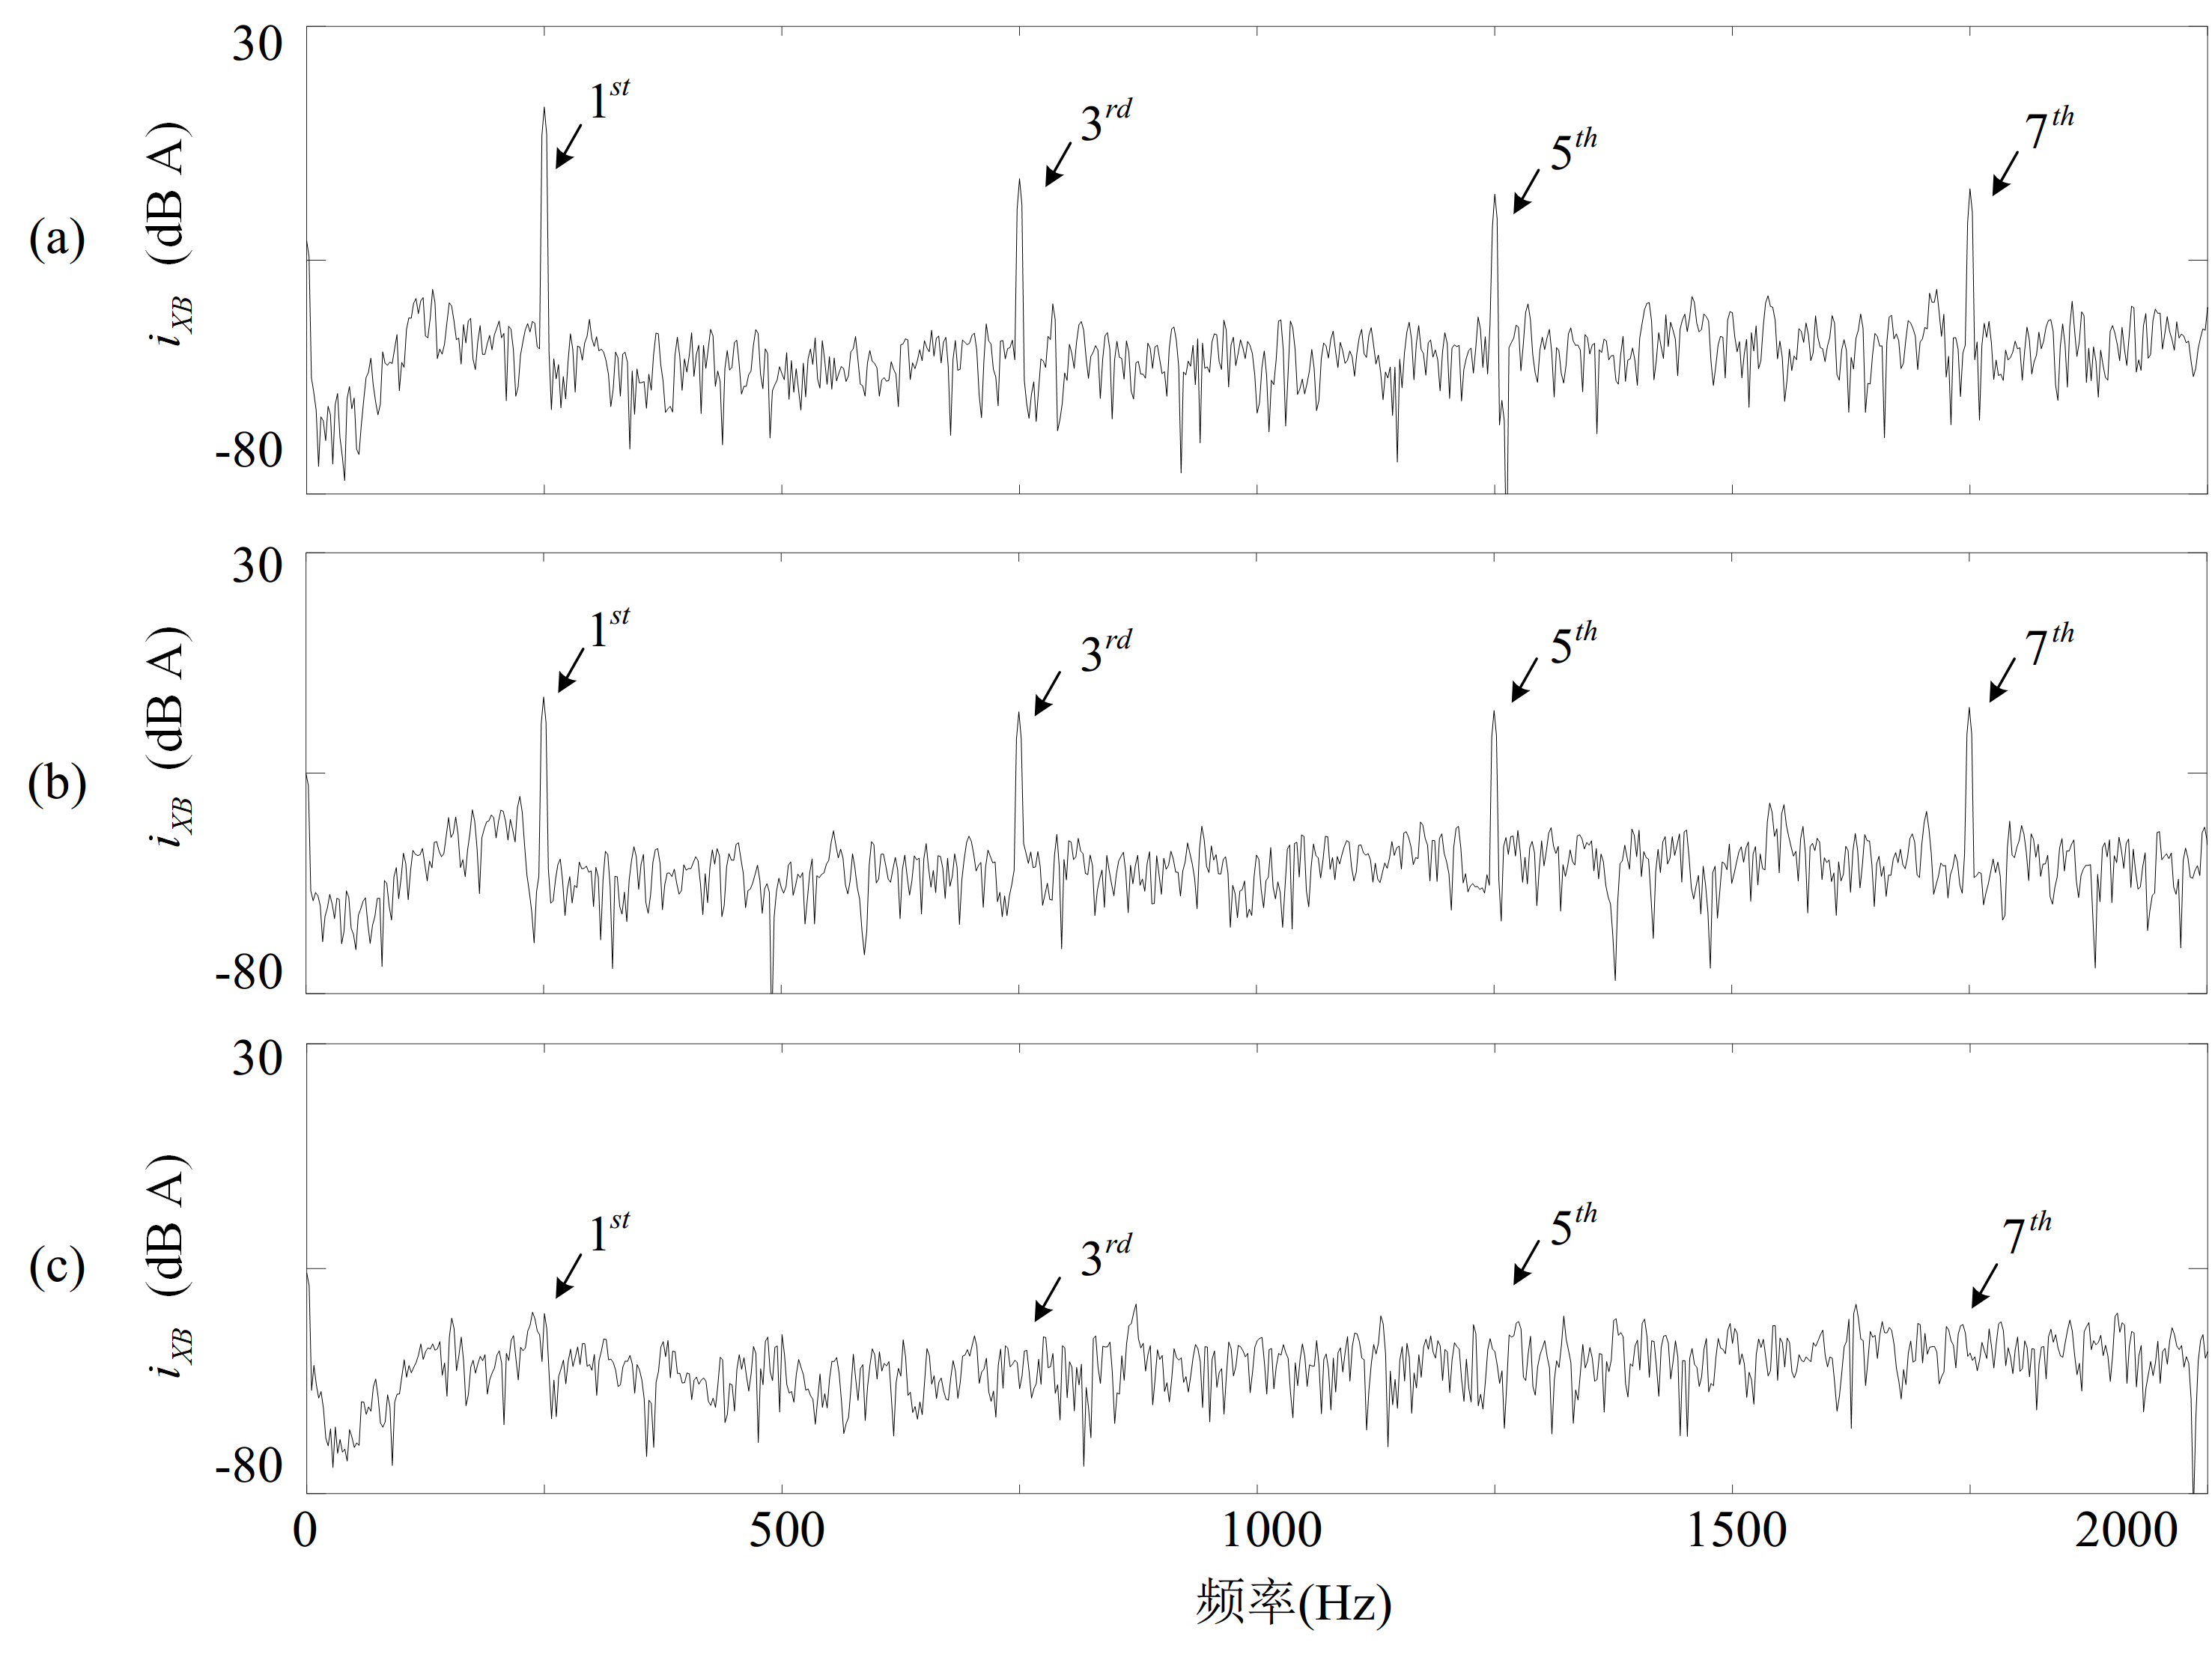
\includegraphics[scale=1.0]{5-orc_current_fft.png}
	\caption{转子250Hz时的线圈电流频谱实验测量结果,a)PID控制,b)PID+传统整数次重复控制器,c)PID+零相移奇数次重复控制器}
	\label{fig:5-orc_current_fft}
\end{figure}

为了定量分析零相移奇数次重复控制器在各个谐波频率处的抑制能力,直观的方法是对\autoref{fig:5-orc_current}的时域波形做傅里叶频谱分析,观察时域电流的频谱。\autoref{fig:5-orc_current_fft}.a显示在仅有PID控制下,由质量不平衡和传感器误差引入的谐波电流的一、三、五、七次谐波的幅值分别是2.8dB、-12.5dB、-15.8dB和-14.7dB。\autoref{fig:5-orc_current_fft}.b中,加入传统整数次重复控制器之后,幅值分别下降到-12.7dB、-16.1dB、-15.8dB和-15.1dB。可以看出,随着谐波频率的升高,传统整数次重复控制器的抑制能力逐渐减弱。\autoref{fig:5-orc_current_fft}.c中,加入零相移奇数次重复控制器之后,谐波幅值分别下降至-40.0dB、-56.7dB、-48.4dB和-48.8dB,下降程度均超过90\%。

\begin{table}[htb]
  \caption[250Hz时磁悬浮轴承系统功率实验测量结果]{250Hz时磁悬浮轴承系统功率实验测量结果\label{tab:amb_power}}
  \begin{tabular}{cc}
    \toprule
    控制策略 & 功率消耗 \\
    \midrule
    PID & 142.3W\\
    PID+传统整数次重复控制器 & 95.3W\\
    PID+零相移奇数次重复控制器 & 58.2W\\
    \bottomrule
  \end{tabular}
\end{table}

\autoref{tab:amb_power}显示了磁悬浮轴承系统在转子250Hz悬浮运转时的功率消耗。仅有PID控制时,系统功率消耗为142.3W;当加入传统整数次重复控制器之后,功率消耗下降到95.3W;当加入零相移奇数次重复控制器之后,功率消耗则下降到58.2W。该对比结果显示奇数次重复控制器比传统整数次重复控制器更能降低系统的功率消耗。

\begin{figure}
	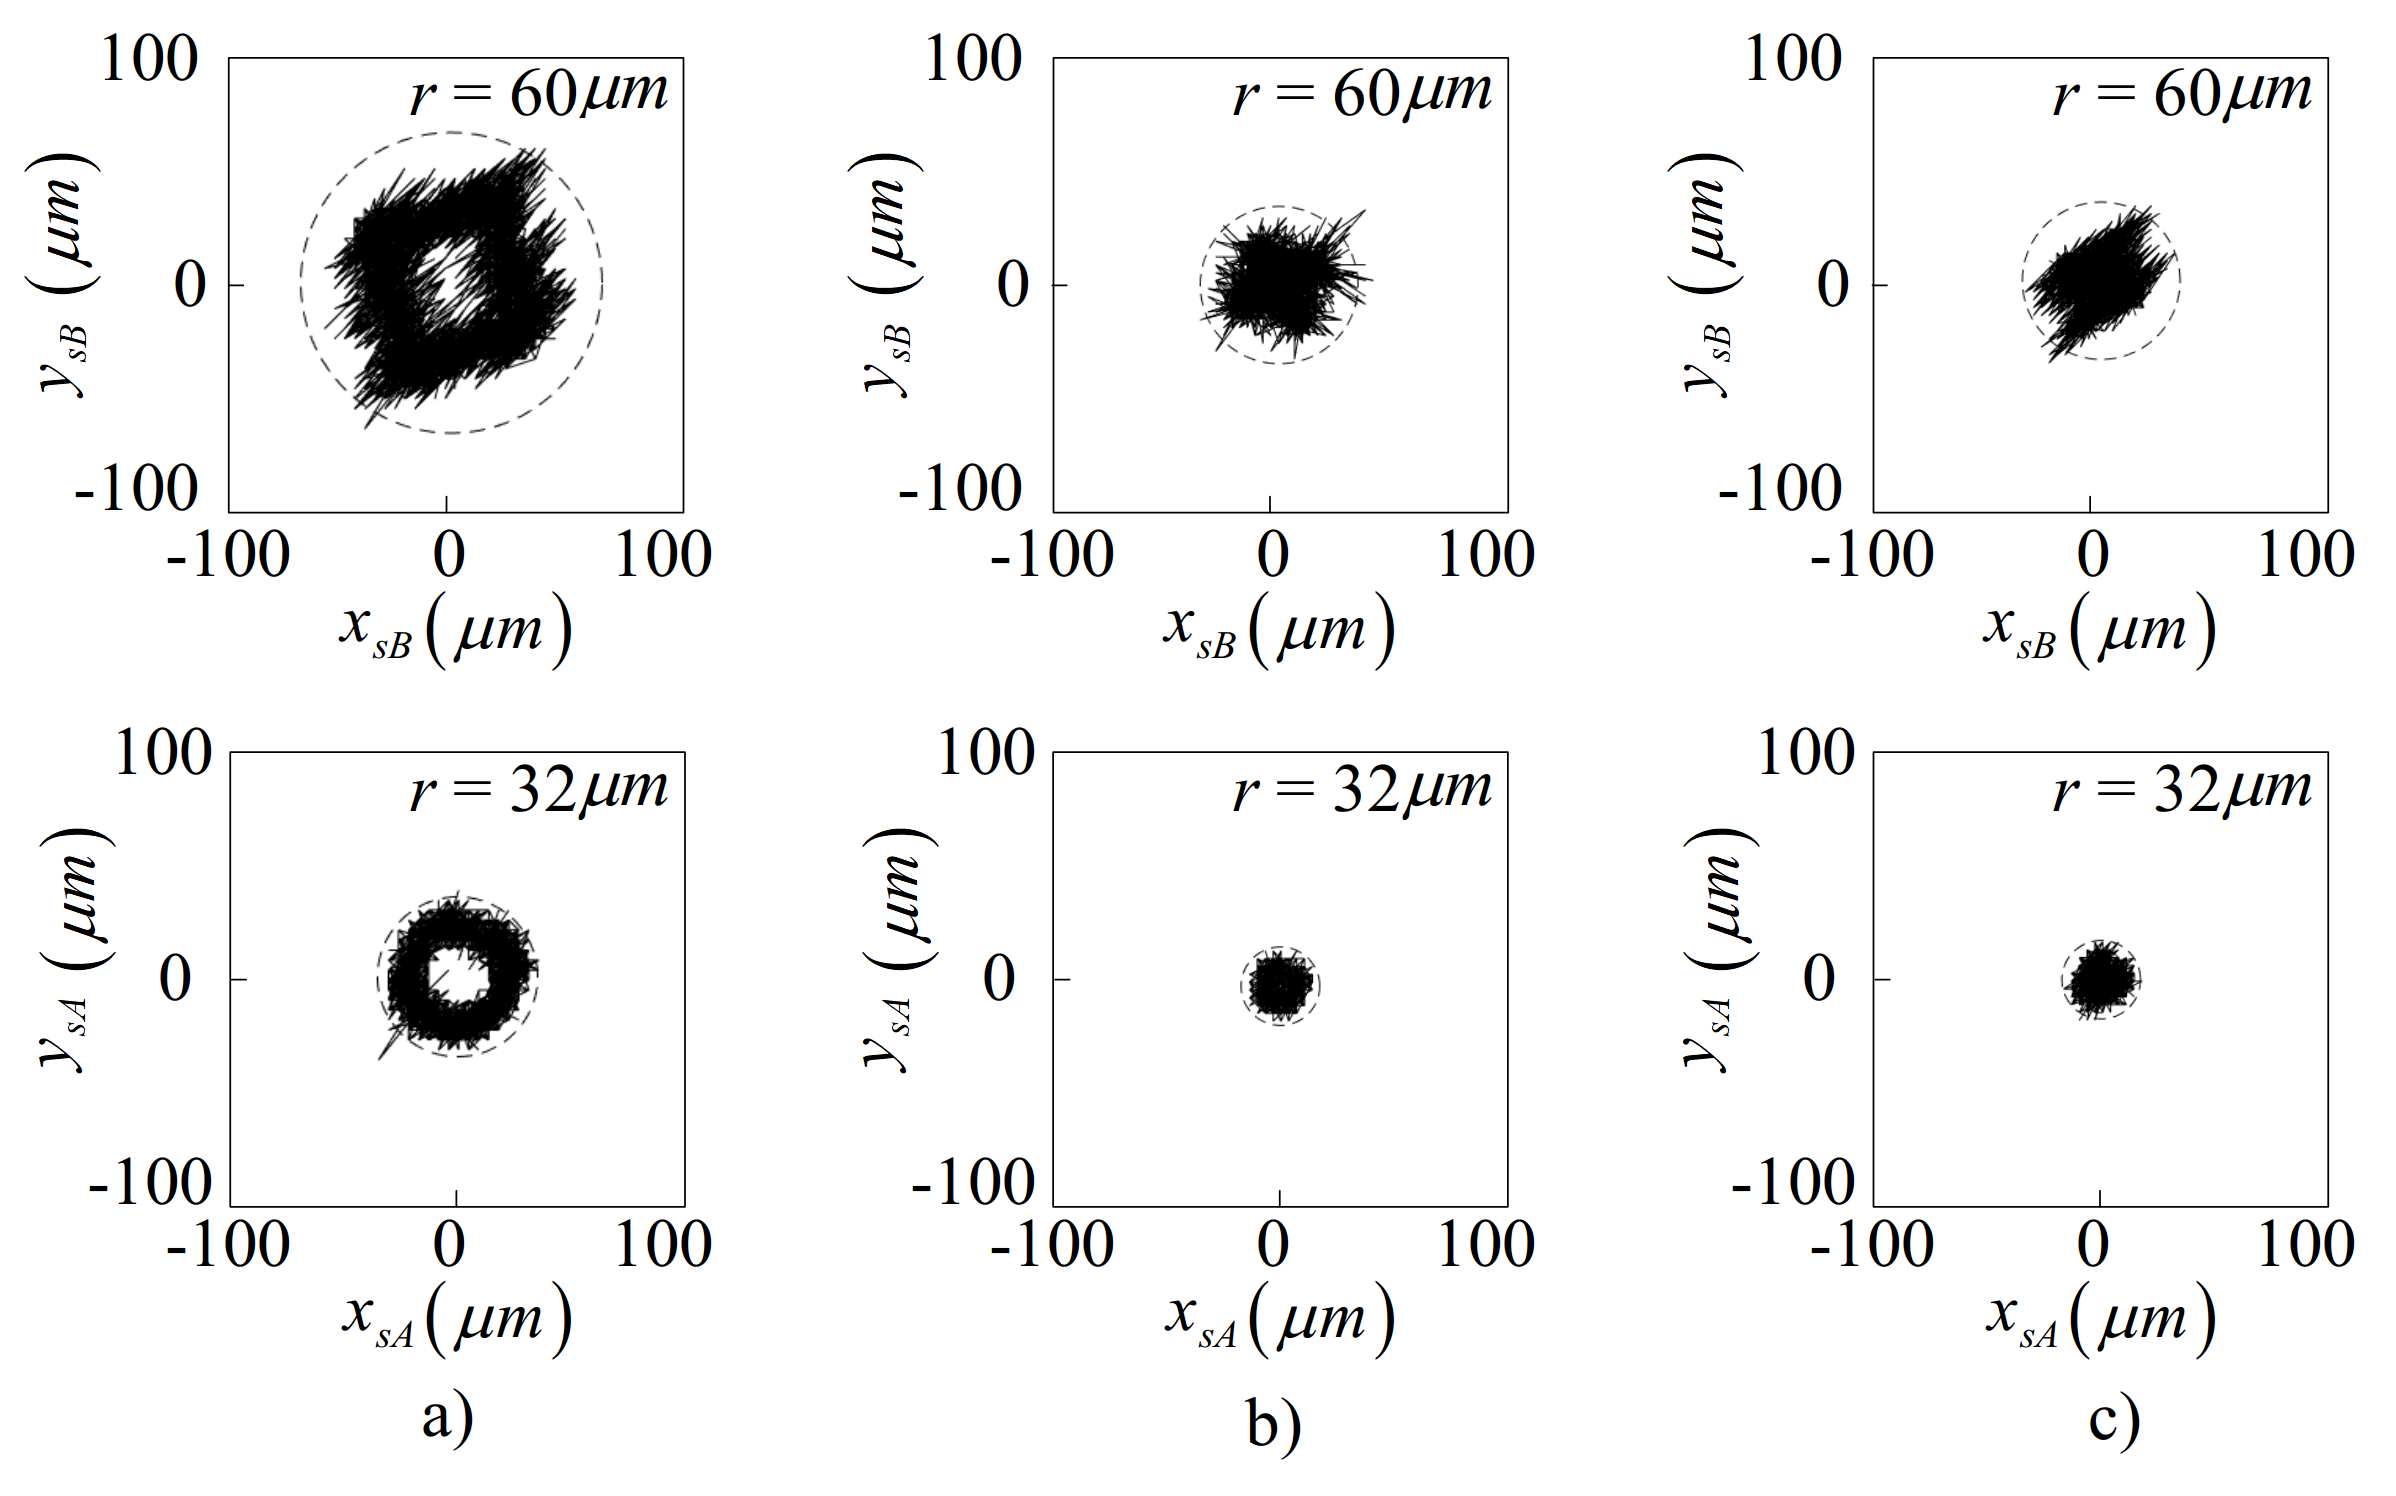
\includegraphics[scale=1.0]{5-rotor_locus.png}
	\caption{转子250Hz时两端的轴心轨迹实验测量结果,a)PID控制,b)PID+传统整数次重复控制器,c)PID+零相移奇数次重复控制器}
	\label{fig:5-rotor_locus}
\end{figure}

除功率消耗降低之外,零相移奇数次重复控制器带来的好处是提升转子的回转精度。此处的轴心轨迹通过位移传感器测得的转子位移绘制而成,轴心轨迹的半径记为$r$。\autoref{fig:5-rotor_locus}.a显示仅有PID控制下,转子在A端磁悬浮轴承处的轴心轨迹为$60\mu m$,在B端磁悬浮轴承处的轴心轨迹为$32\mu m$。\autoref{fig:5-rotor_locus}.b中,加入传统整数次重复控制器之后,转子在A端磁悬浮轴承处的振动幅值下降到$40\mu m$,在B端磁悬浮轴承处的振动幅值下降到$20\mu m$。\autoref{fig:5-rotor_locus}.c中,加入零相移奇数次重复控制器之后,转子在A端和B端磁悬浮轴承处的振动幅值同样下降到$40\mu m$和$20\mu m$。该实验现象说明传统整数次重复控制器和零相移奇数次重复控制器具有相同的提升转子回转精度的能力。

\begin{figure}
	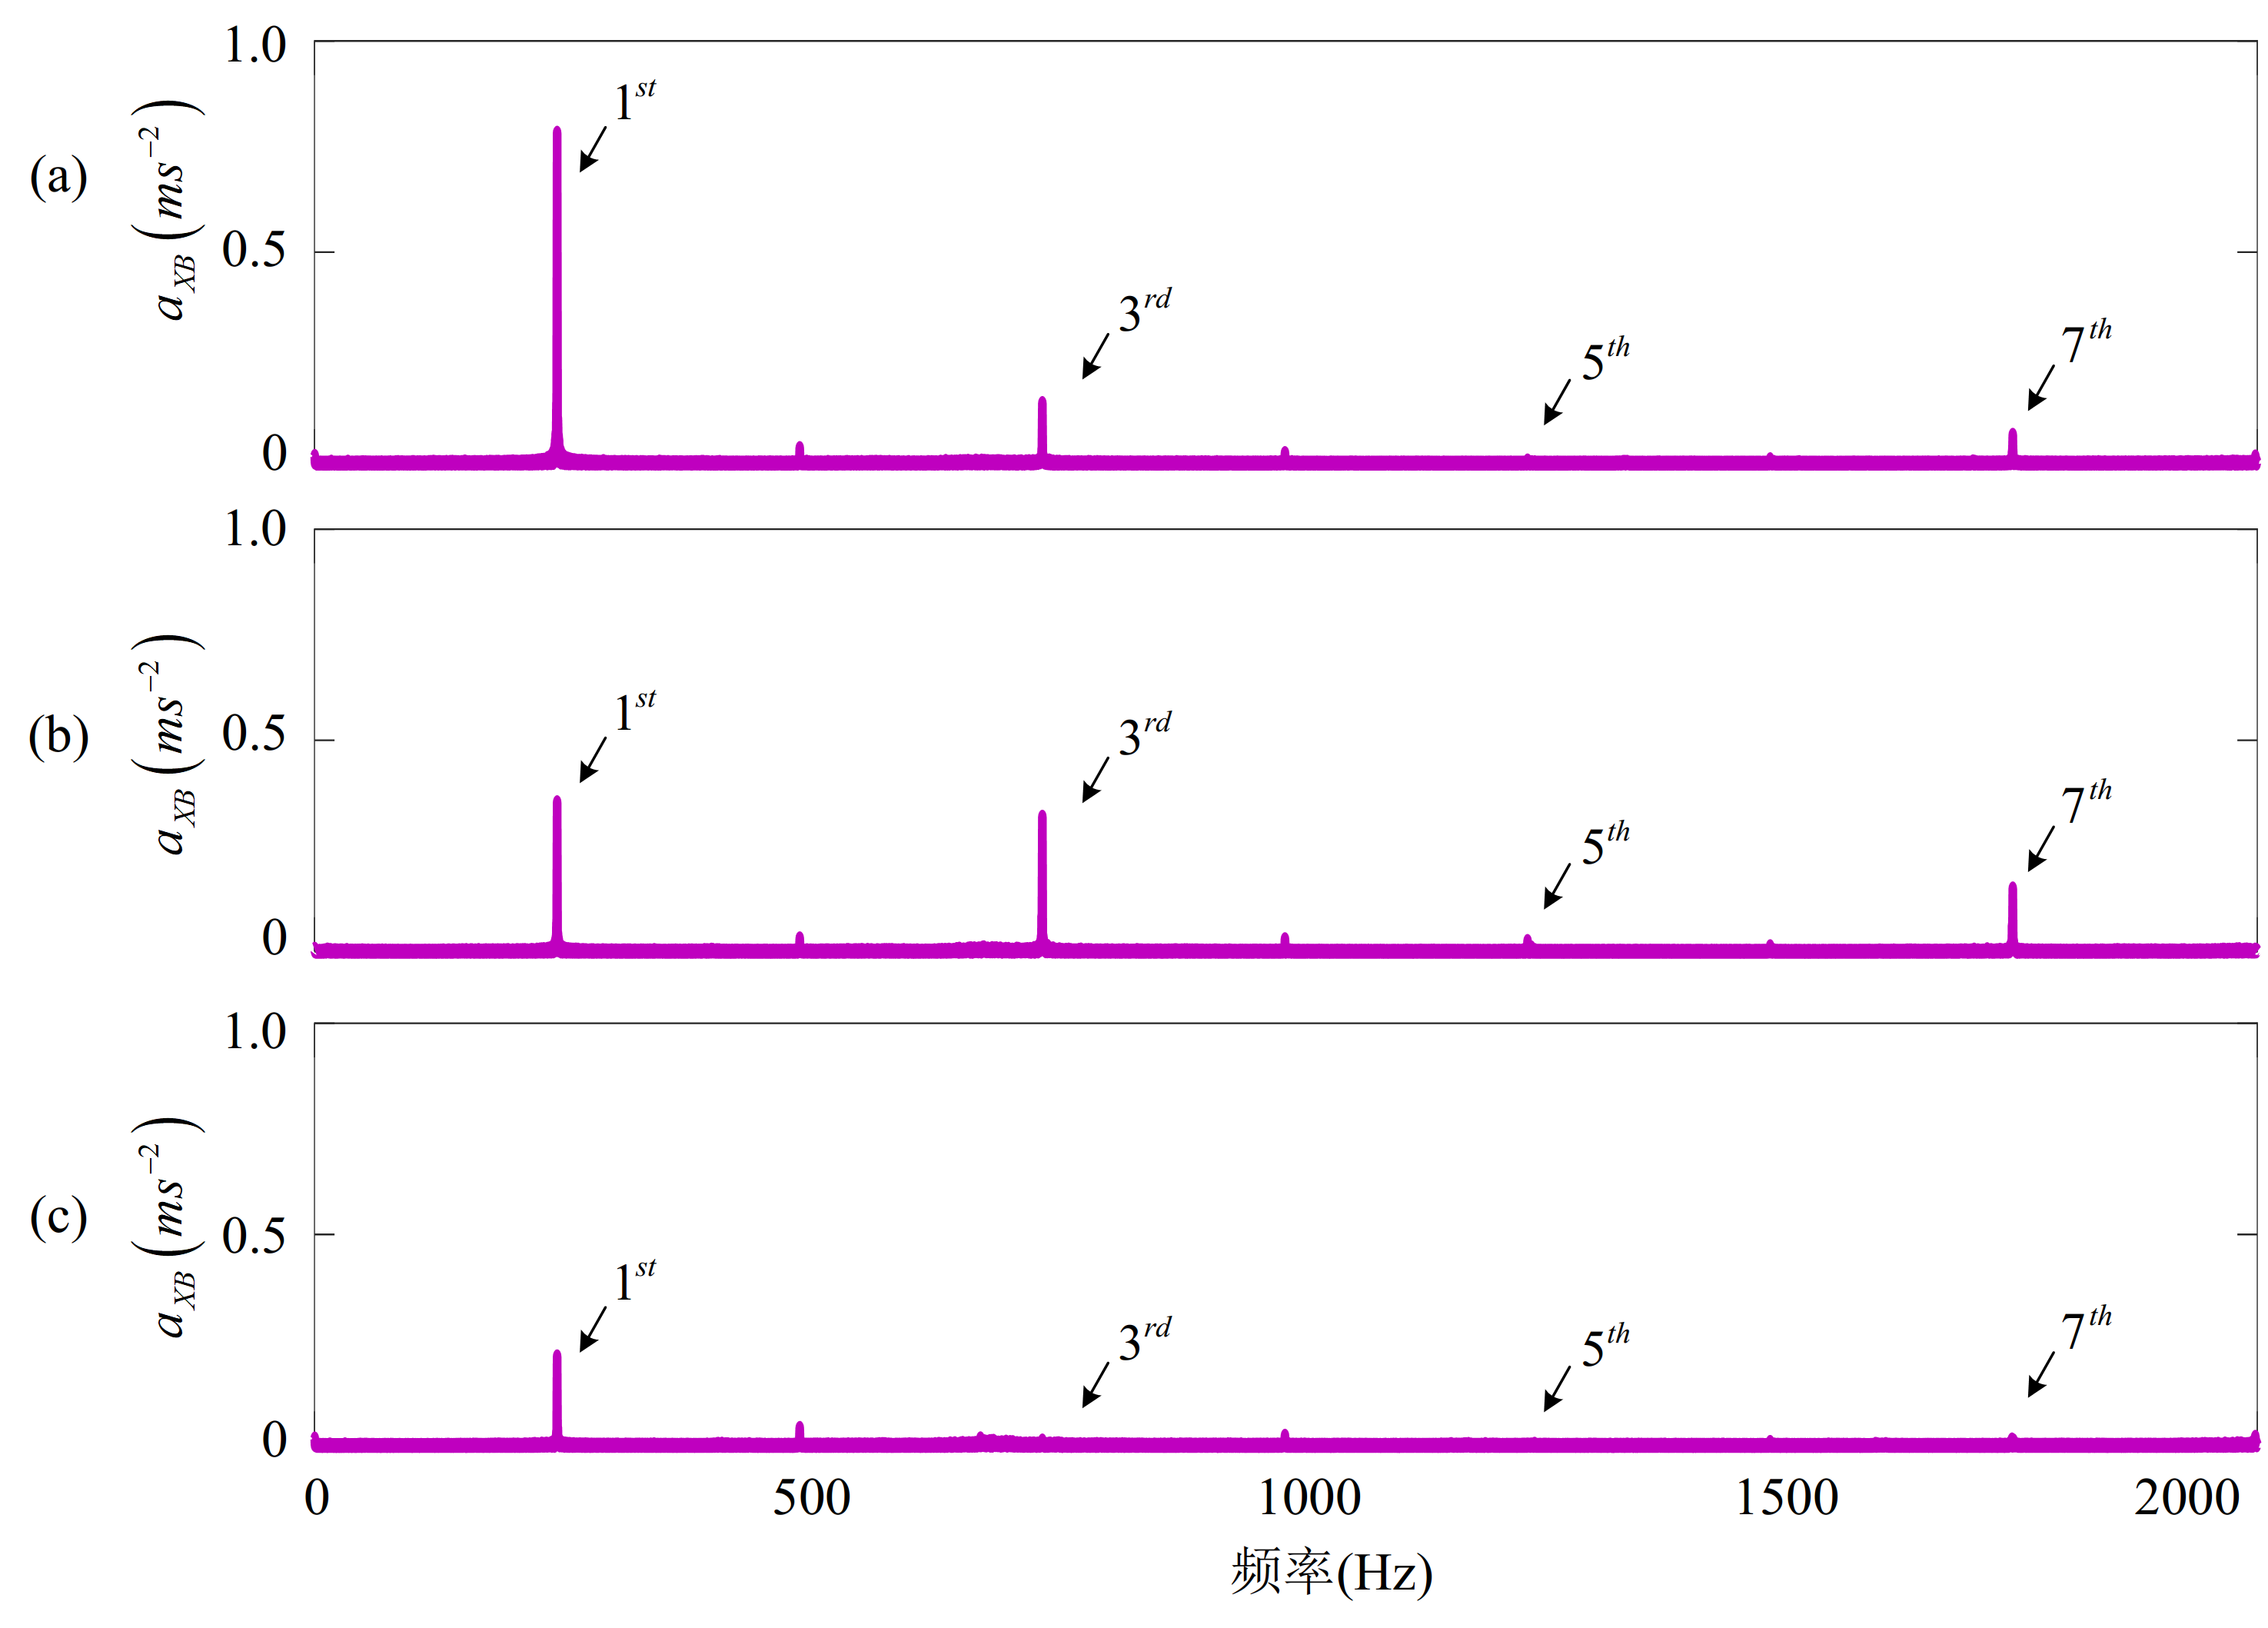
\includegraphics[scale=1.0]{5-orc_acc.png}
	\caption{转子250Hz时定子基座的加速度实验测量结果,a)PID控制,b)PID+传统整数次重复控制器,c)PID+零相移奇数次重复控制器}
	\label{fig:5-orc_acc}
\end{figure}

为了验证实际应用过程中零相移奇数次重复控制器对整机振动力的抑制能力,我们使用加速度传感器来测量磁悬浮电机机壳上的振动加速度。
\autoref{fig:5-orc_acc}显示了转子250Hz时定子基座的加速度实验测量结果。\autoref{fig:5-orc_acc}.a显示当仅有PID控制时,一、三、五、七次谐波频率处的振动幅值为$0.782ms^{-2}$、$0.142ms^{-2}$、$0.002ms^{-2}$和$0.066ms^{-2}$。\autoref{fig:5-orc_acc}.b中,加入传统整数次重复控制器之后,与转速同频的振动幅值下降到$0.352ms^{-2}$,然而三、五、七次谐波频率处的振动幅值上升到$0.318ms^{-2}$、$0.024ms^{-2}$、$0.148ms^{-2}$。这是因为尽管三、五、七次谐波频率处的电流幅值有轻微的衰减,其相位可能发生剧烈的改变,因此使得磁悬浮力增大。\autoref{fig:5-orc_acc}.c中,加入零相移奇数次重复控制器之后,一、三、五、七次谐波频率处的振动幅值下降到$0.210ms^{-2}$、$0.011ms^{-2}$、$0.001ms^{-2}$和$0.014ms^{-2}$,与转速同频的振动力下降了超过70\%,其它谐波频率处的振动力几乎下降到零。该实验现象说明传统整数次重复控制器的谐波抑制能力随着频率升高而减弱,与之对比的是零相移奇数次重复控制器可以有效抑制所有频率处的谐波。

\section{基于零相移奇数次重复控制器的现场动平衡实验}
在进行本实验前,实验样机已在动平衡机上完成去重式转子动平衡,残余不平衡质量较小,其旋转时在转子位移中产生的振动幅值较低。为测试验证本文提出的基于现场动平衡的振动控制方法、评估实验效果,本人在转子两端分别增加一定配重,用于模拟转子的初始不平衡质量。再使用本文提出的基于谐波抑制的现场动平衡方法辨识该不平衡质量,并通过增重的方式进行补偿,分析现场动平衡前后转子振动量级。

\subsection{增加初始配重}

实验样机的转子在动平衡机上完成去重式动平衡之后,250Hz运转时磁悬浮轴承位移波形如\autoref{fig:5-s3-x-w0-pid}所示。径向自由度位移振动幅值约$30\mu m$,该振动量级较小。由于本文提出的新型现场动平衡算法用于辨识转子不平衡质量以及补偿该不平衡质量,在振动量级较小时难以对比观察现场动平衡前后转子振动量级,因此增加配重,使转子初始不平衡质量更大,便于测试现场动平衡算法。增加配重之后,250Hz运转时磁悬浮轴承位移波形如\autoref{fig:5-s3-x-w1-pid}所示。

\begin{figure}[htb]  
	\subfloat[初始不平衡质量引起的位移振动\label{fig:5-s3-x-w0-pid}]{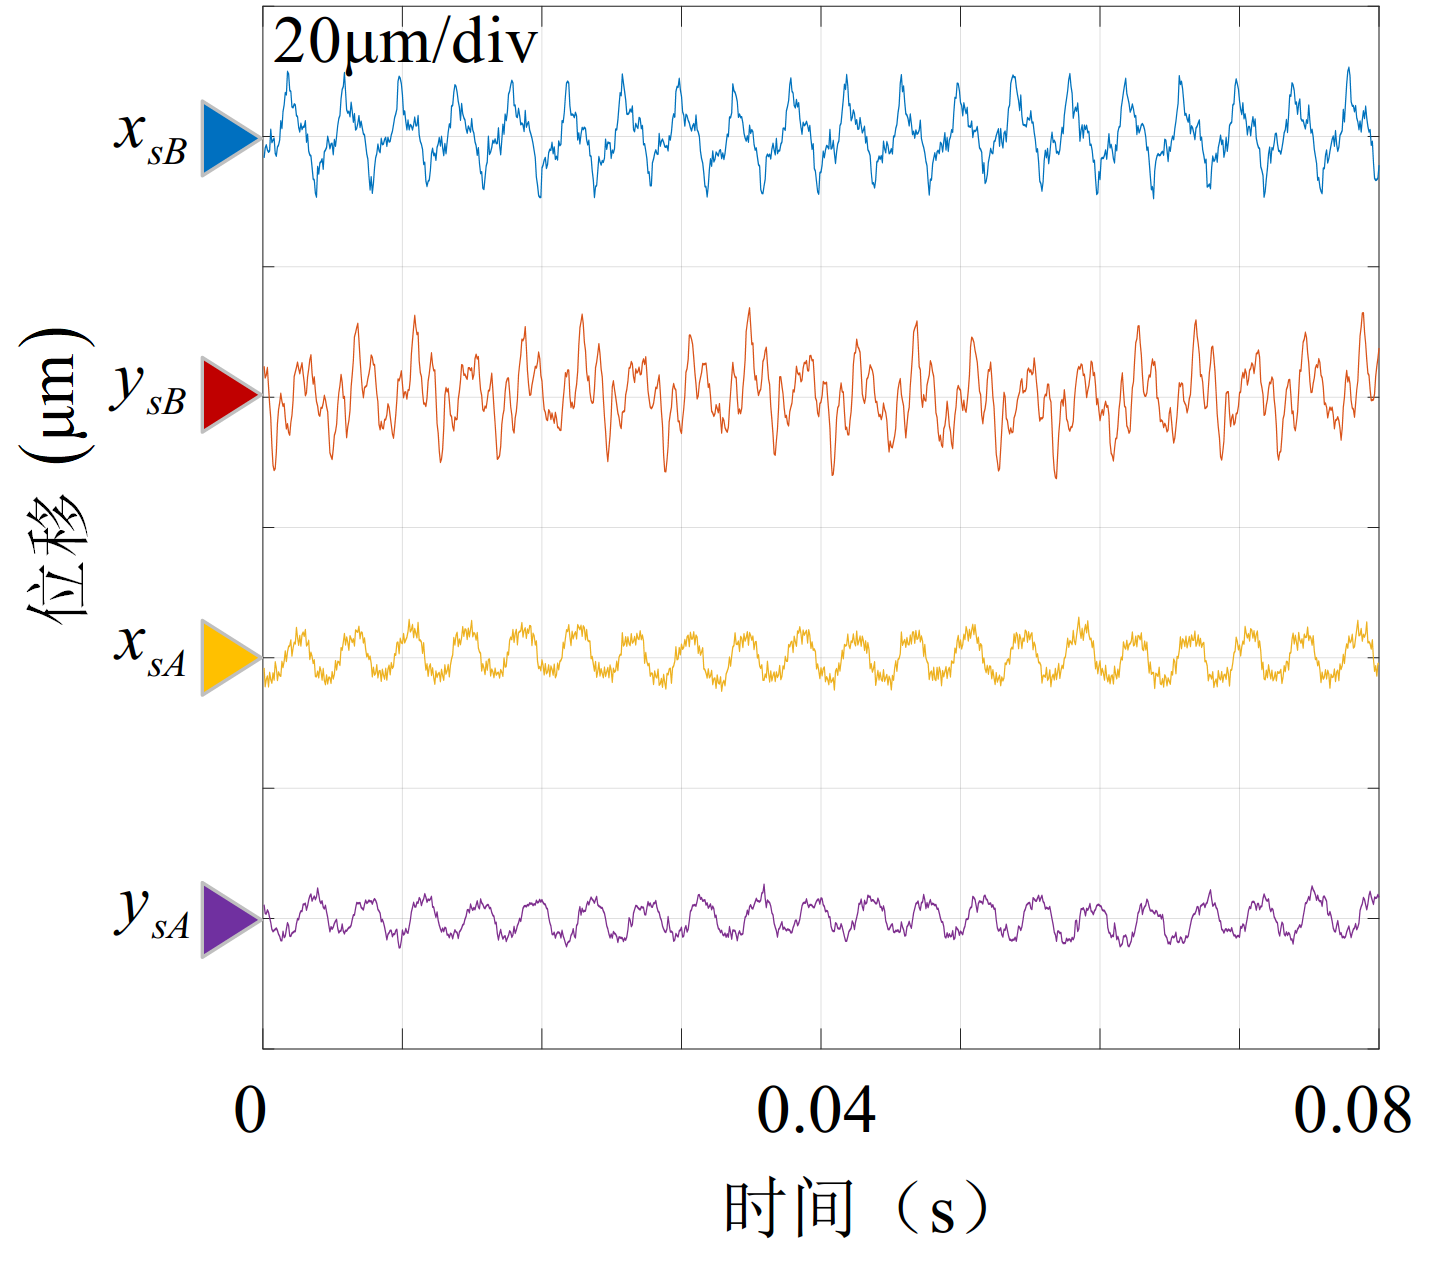
\includegraphics[scale=1.0]{5-s3-x-w0-pid.png}}\quad  
	\subfloat[增加配重后转子不平衡质量引起的位移振动\label{fig:5-s3-x-w1-pid}]{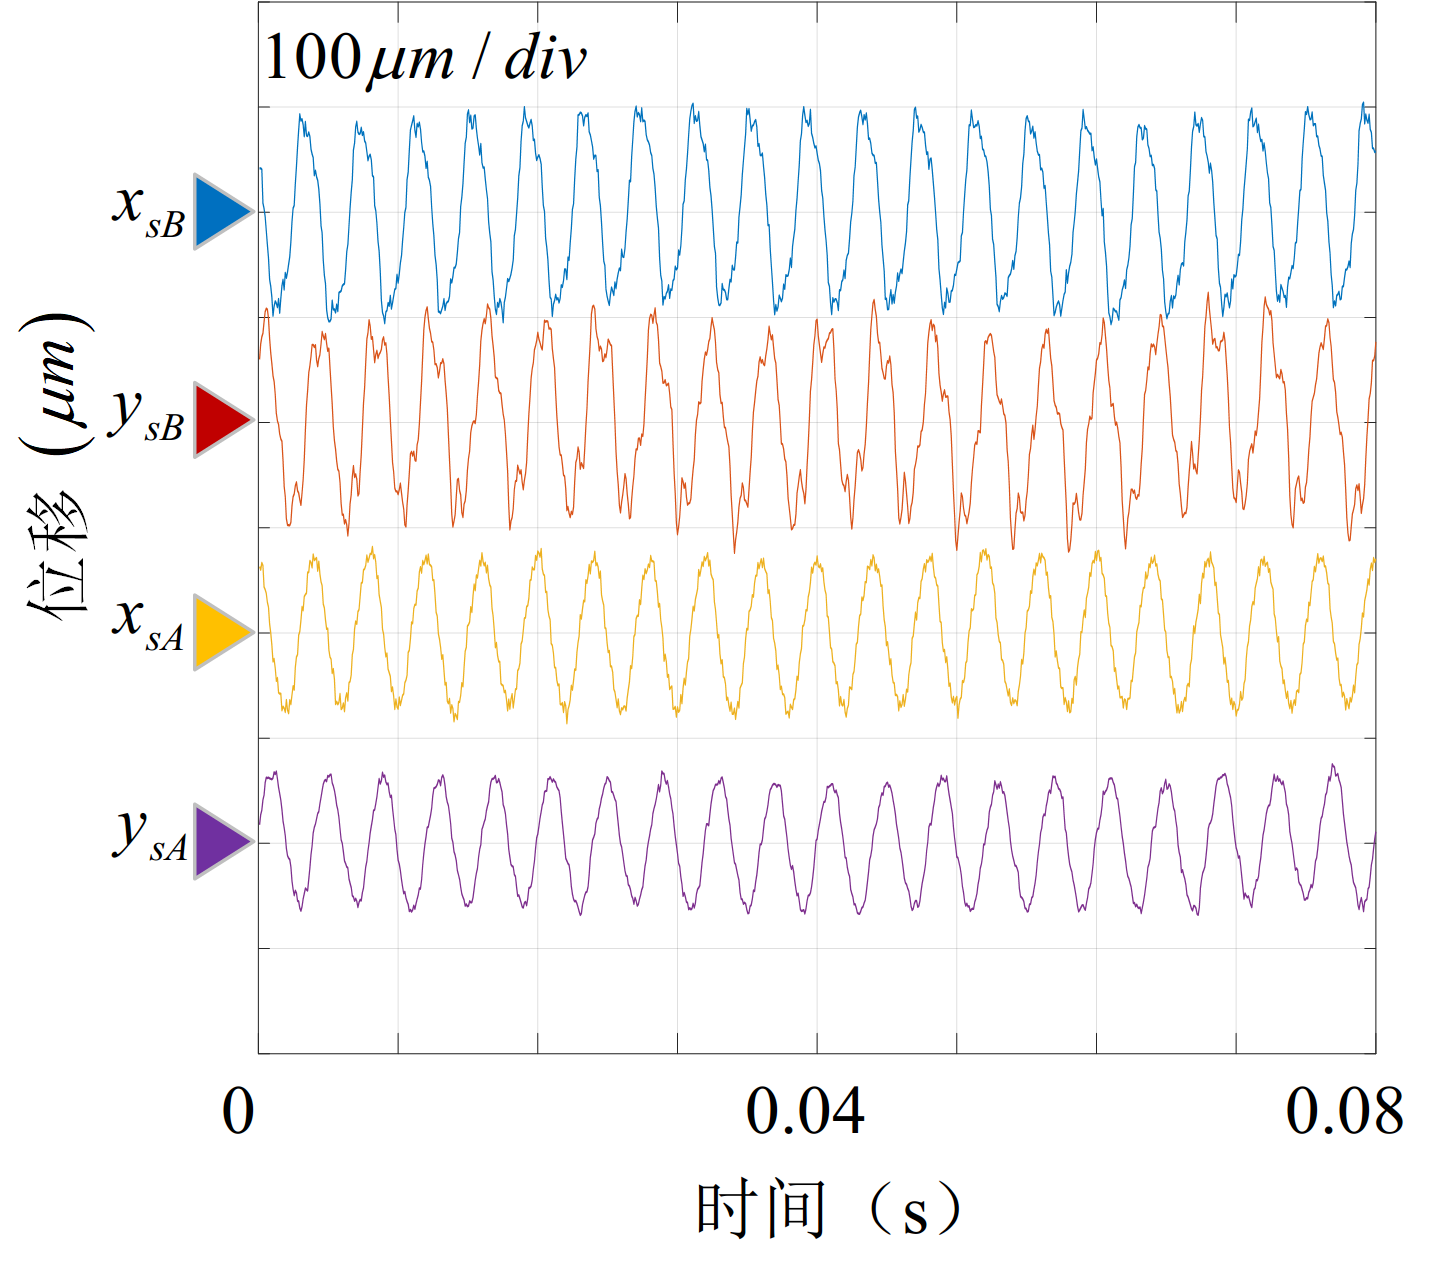
\includegraphics[scale=1.0]{5-s3-x-w1-pid.png}}  		\caption{转子不平衡质量引起的位移振动}  \label{fig:5-s3-x-w0/w1}\end{figure}

两端的配重盘尺寸一致,靠近边沿处有一圈36个螺丝孔,每两个孔之间间距$10^{\circ}$。每个孔上可以通过螺丝固定数量不等的垫片在配重盘上,达到增重的目的。增加初始配重质量的幅值和相位分别如\autoref{tab:nf_orc_w1}所示。

\subsection{实现零电流控制}

一、传统方案:使用陷波器法实现零电流控制

根据\autoref{fig:5-sens_x}、\autoref{fig:5-sens_y}、\autoref{fig:5-sens_u}和\autoref{fig:5-sens_v}所示的输出敏感度函数,转子在70Hz$\sim$100Hz附近增益幅值最大,说明在该频率段转子的稳定性能较差。考虑转子到高速时各自由度输出敏感度增益较小,且相位变化平缓,因此下文所涉及的现场动平衡实验均选取250Hz作为位移波形采集频率点。依据第四章阐述的陷波器参数设计方法,从输出敏感度函数曲线上获取250Hz处的输出敏感度相位并设计陷波器参数如\autoref{tab:250_S0_phase}所示。根据实验现象,从零逐渐增加陷波器参数$k_f$,当$k_f = 50$时,振动抑制效果良好。

\begin{table}[htb]
  \caption[径向各自由度在250Hz的输出敏感度相位]{径向各自由度在250Hz的输出敏感度相位\label{tab:250_S0_phase}}
  \begin{tabular}{ccc}
    \toprule
    自由度 & 250Hz处输出敏感度函数相位 & $\theta _f$ \\
    \midrule
    $X_A$ & $0^{\circ}$ & $0^{\circ}$\\
    $Y_A$ & $1^{\circ}$ & $-1^{\circ}$\\
    $X_B$ & $2^{\circ}$ & $-2^{\circ}$\\
    $Y_B$ & $0^{\circ}$ & $0^{\circ}$\\
    \bottomrule
  \end{tabular}
\end{table}

\begin{figure}[htb]  
	\subfloat[现场动平衡前PID控制下线圈电流时域波形\label{fig:5-s3-i-w1-pid}]{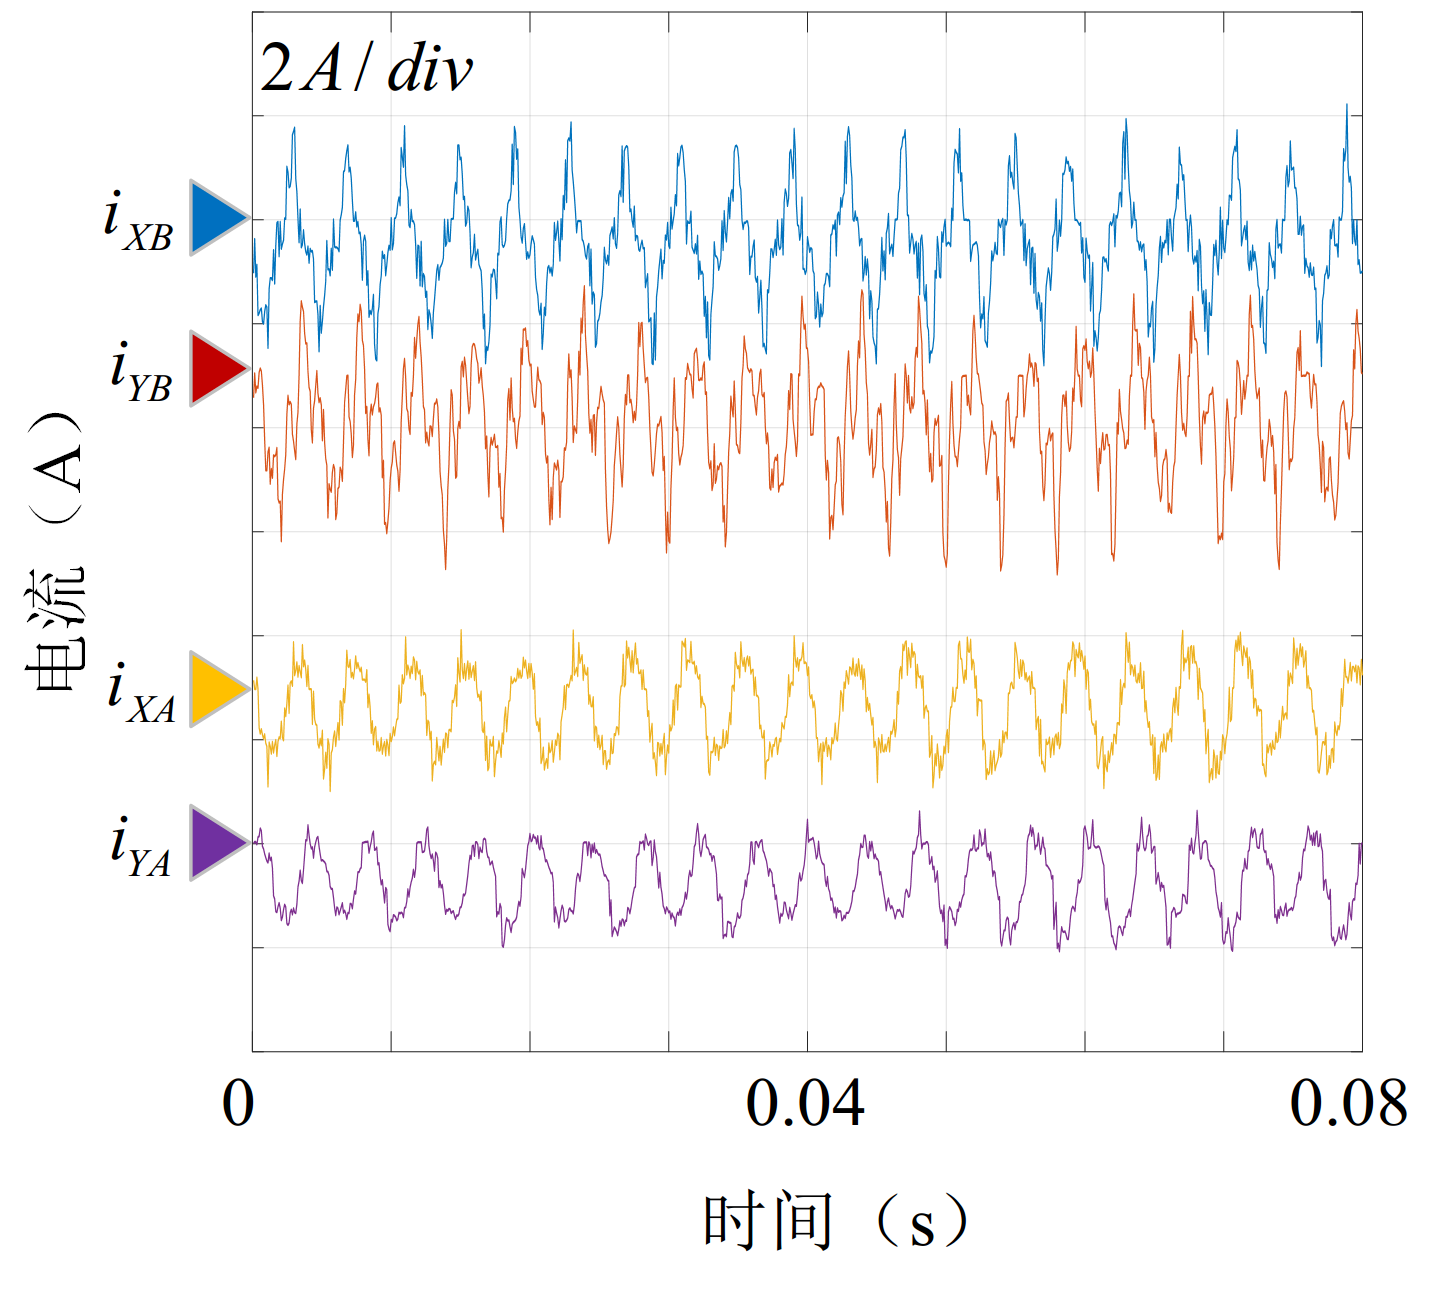
\includegraphics[scale=1.0]{5-s3-i-w1-pid.png}}\quad  
	\subfloat[现场动平衡前PID+陷波器控制下线圈电流时域波形\label{fig:5-s3-i-w1-pid-nf}]{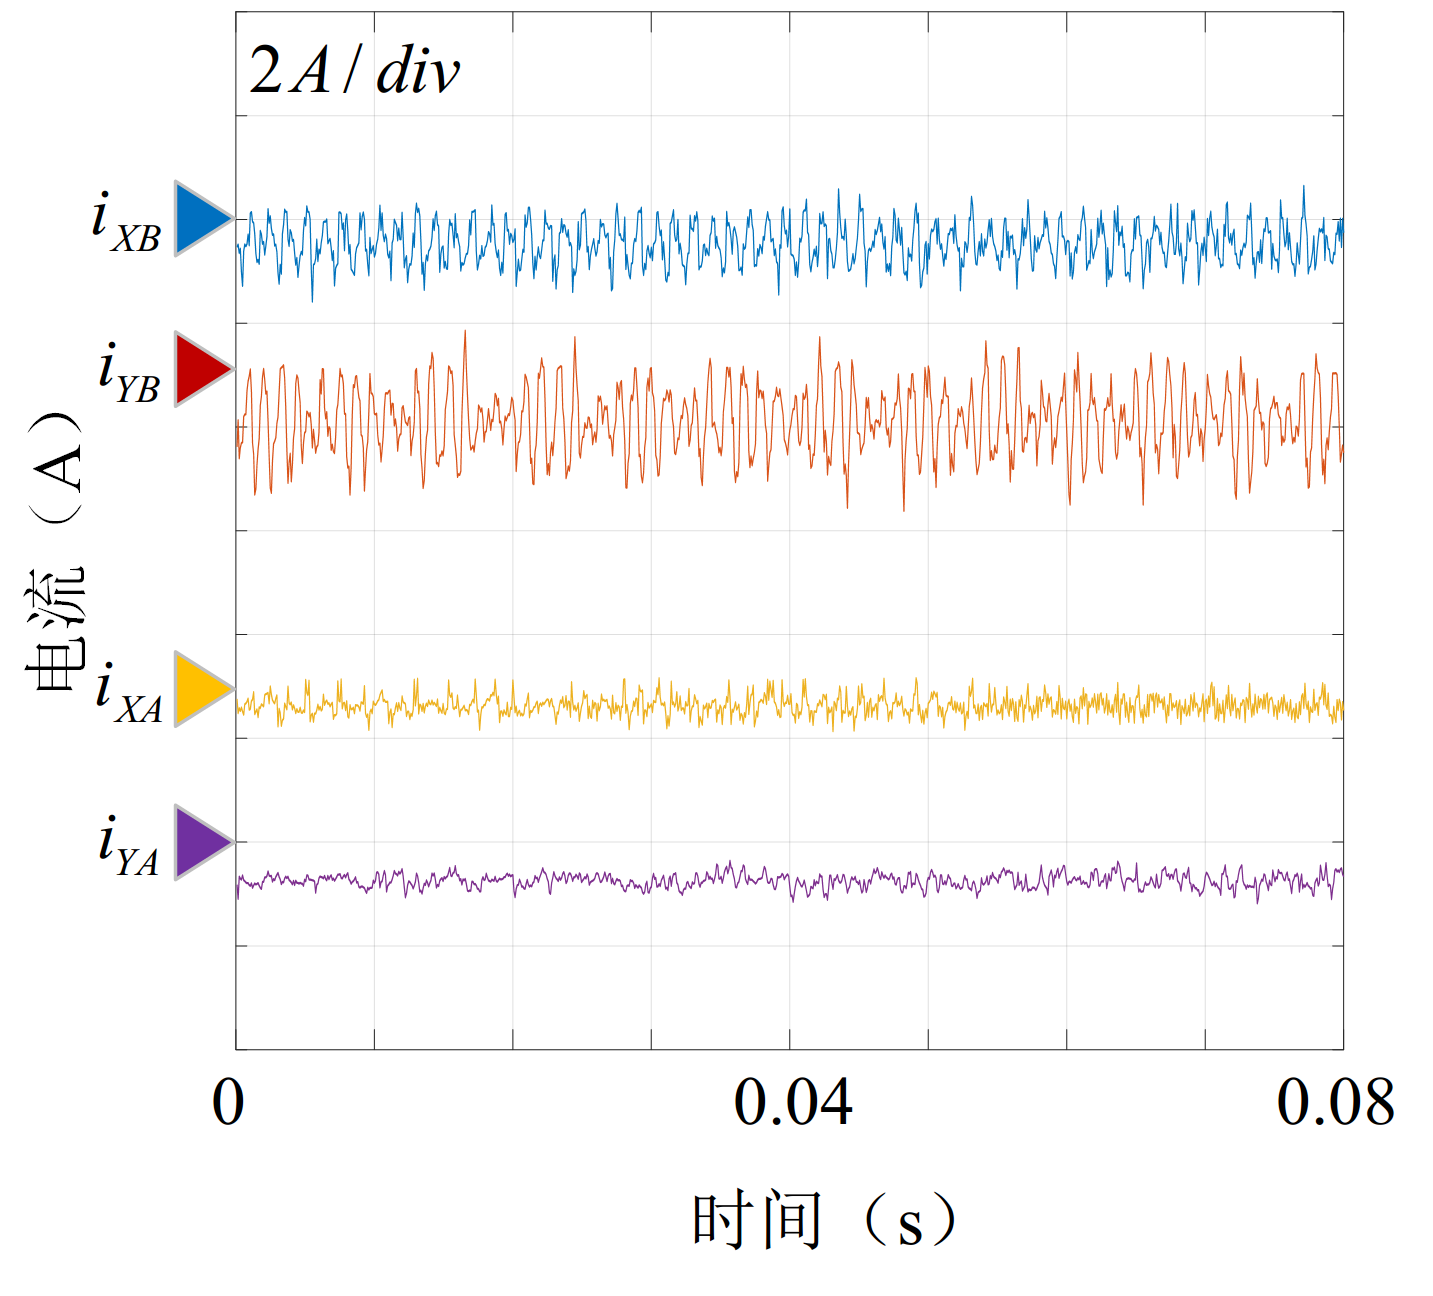
\includegraphics[scale=1.0]{5-s3-i-w1-pid-nf.png}}  
	\caption{现场动平衡前加入陷波器前后线圈电流时域波形}  \label{fig:5-s3-i-w1-pid_nf}\end{figure}

\begin{figure}
	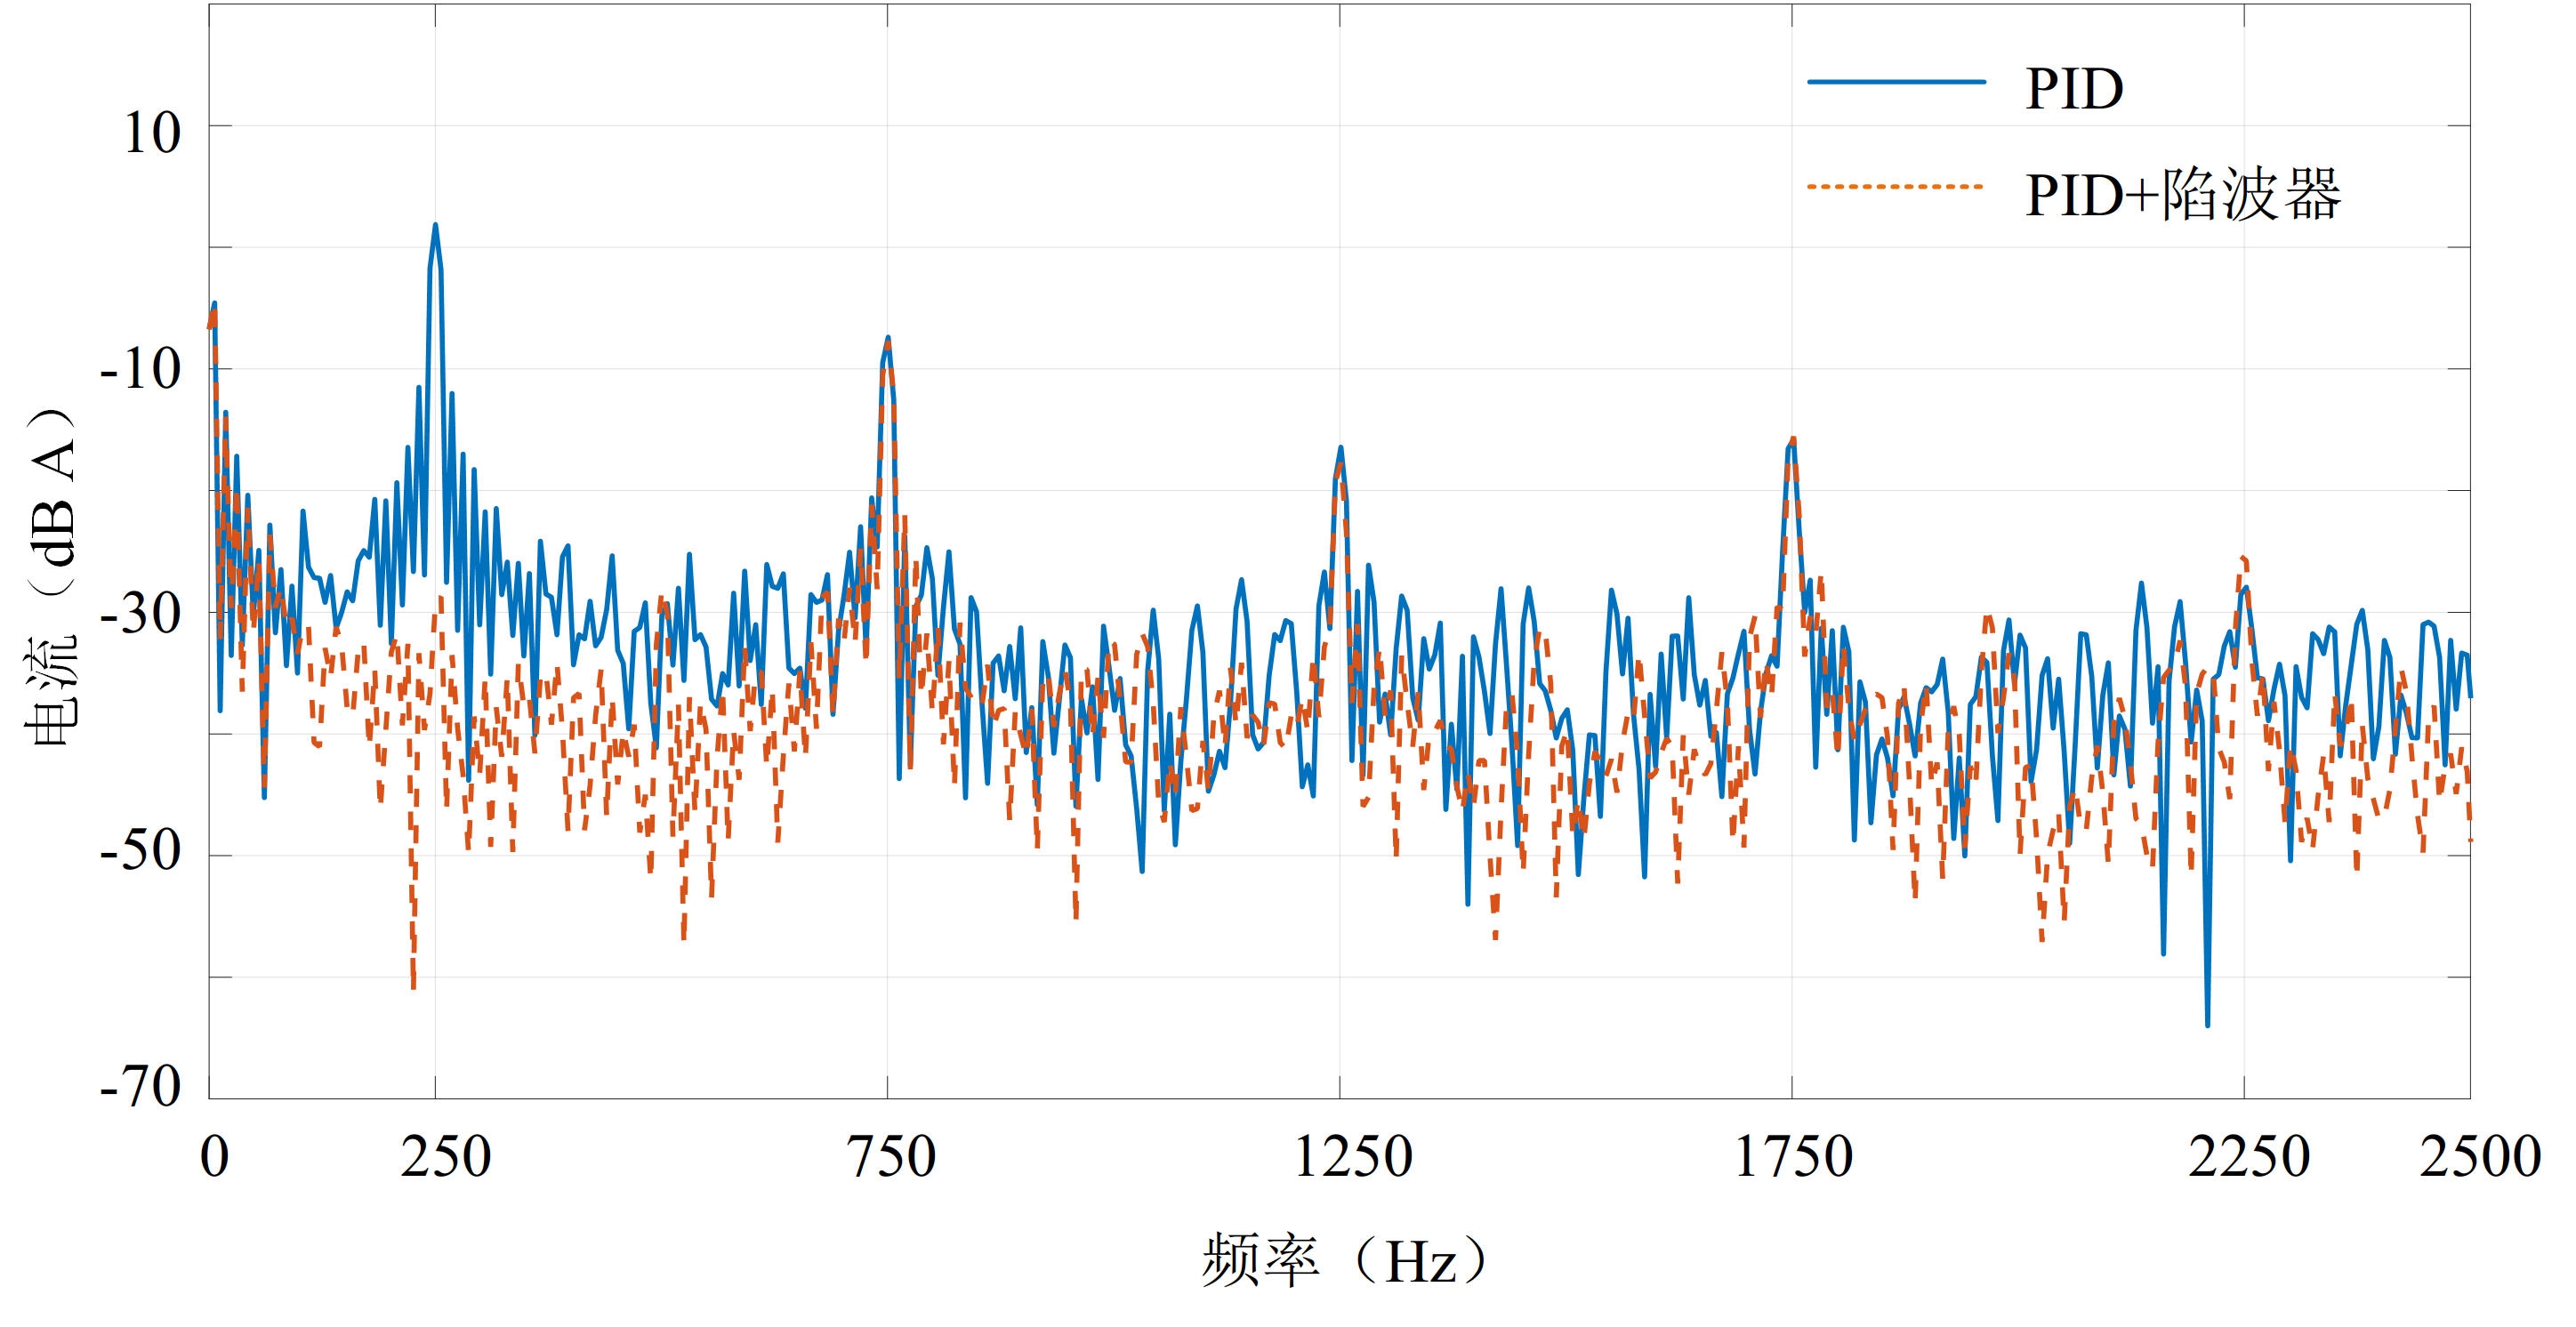
\includegraphics[scale=1.0]{5-s3-i_f-w1-pid_nf.png}
	\caption{现场动平衡前加入陷波器前后$i_{xB}$频谱}
	\label{fig:5-s3-i_f-w1-pid_nf}
\end{figure}

\autoref{fig:5-s3-i-w1-pid_nf}显示了进行现场动平衡之前加入陷波器前后线圈电流时域波形。考虑到四个径向通道控制策略和控制对象模型一致,因此仅分析其中一个自由度的电流的频谱图像即可反应加入陷波器对控制电流的影响,此处选取$i_{xB}$电流频谱分析。\autoref{fig:5-s3-i-w1-pid}显示,质量不平衡引起控制电流振动,各自由度的控制电流幅值均较大。\autoref{fig:5-s3-i-w1-pid-nf}中可以看出,加入陷波器之后控制电流幅值明显衰减。\autoref{fig:5-s3-i_f-w1-pid_nf}可以进一步看到控制电流中包含一、三、五和七次谐波,加入陷波器可以有效抑制同频振动电流:同频电流幅值从约-5dB A下降到约-30dB A,但是三、五和七次谐波的幅值并未显示任何衰减。

加入陷波器后,转子旋转轴趋于惯性轴旋转。由于转子高速旋转式具有自对中效应,转子两端的轴心轨迹半径变小。\autoref{fig:5-s3-x_locus-w1-pid-nf_end}显示了加入陷波器前后转子双端轴心轨迹。加入陷波器前,B端轴心轨迹的半径约为$130 \mu m$,A端的轴心轨迹半径约为$75 \mu m$;加入陷波器后,B端轴心轨迹的半径约为$85 \mu m$,A端的轴心轨迹半径约为$45 \mu m$。

\begin{figure}[htb]  
	\subfloat[现场动平衡前加入陷波器前后B端转子轴心轨迹\label{fig:5-s3-x_locus-w1-pid-nf_bend}]{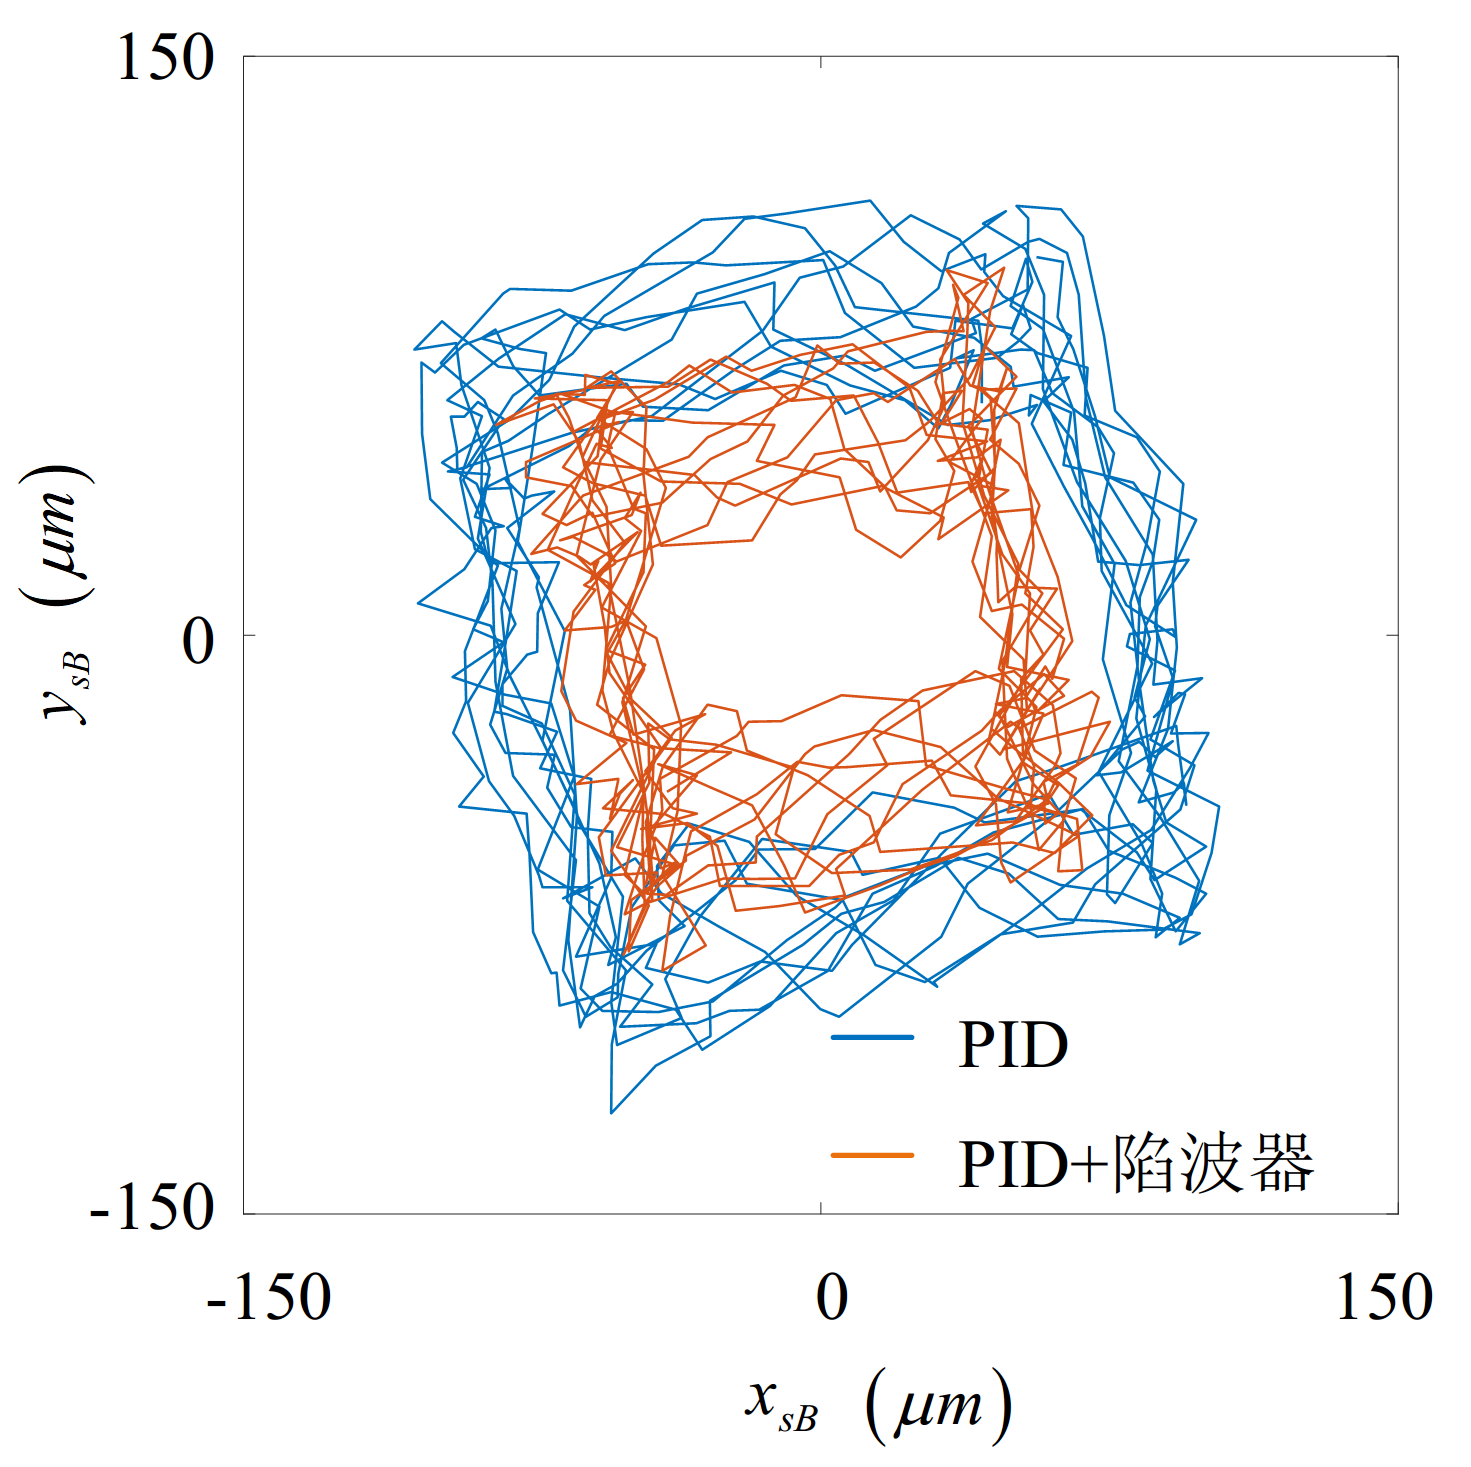
\includegraphics[scale=1.0]{5-s3-x_locus-w1-pid-nf_bend.png}}\quad  
	\subfloat[现场动平衡前加入陷波器前后A端转子轴心轨迹\label{5-s3-x_locus-w1-pid-nf_aend}]{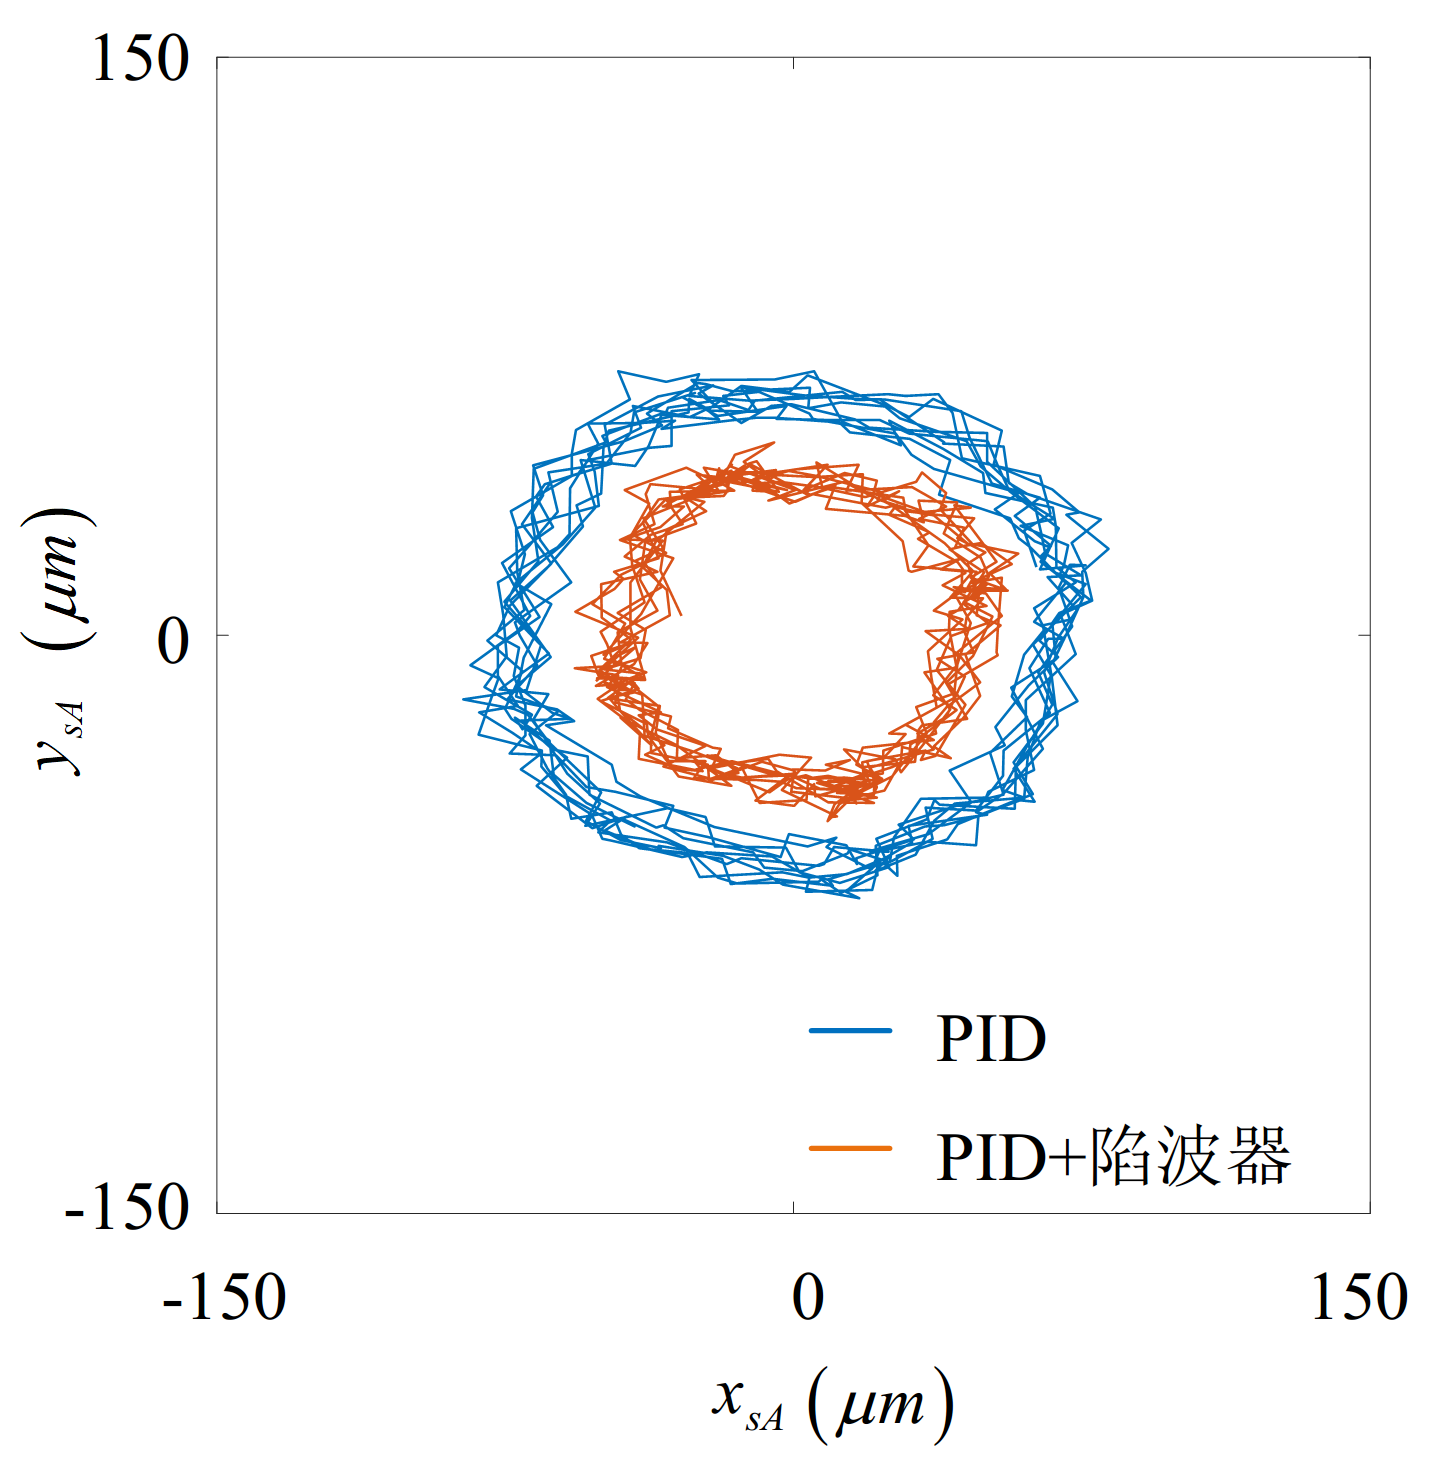
\includegraphics[scale=1.0]{5-s3-x_locus-w1-pid-nf_aend.png}}  
	\caption{现场动平衡前加入陷波器前后转子双端轴心轨迹}  \label{5-s3-x_locus-w1-pid-nf_end}
\end{figure}


二、新型方案:使用零相移奇数次重复控制器实现零电流控制

使用新型基于谐波抑制的转子绕惯性轴旋转方案进行现场动平衡的步骤为:加入零相移奇数次重复控制器抑制控制电流中的谐波,在没有扰动磁悬浮力的作用下,转子将绕惯性轴旋转。此后根据位移波形解析不平衡质量分布,并以增重的方式进行不平衡质量补偿。

\autoref{fig:5-s3-i-w1-pid_orc}显示了现场动平衡前加入重复控制器前后线圈电流时域波形。加入重复控制器后,最大的控制电流幅值从\autoref{fig:5-s3-i-w1-pid}所示的约2A下降到\autoref{fig:5-s3-i-w1-pid-orc}所示的约1A。\autoref{fig:5-s3-i_f-w1-pid_orc}显示了现场动平衡前加入重复控制器前后$i_{sB}$频谱,从此图中可以清楚看出加入重复控制器前控制电流中包含一、三、五和七次谐波成分,加入重复控制器后,一、三、五和七次谐波频率处的尖峰消失,谐波电流被有效消除。

\begin{figure}[htb]  
	\subfloat[现场动平衡前PID控制下线圈电流时域波形\label{fig:5-s3-i-w1-pid_1}]{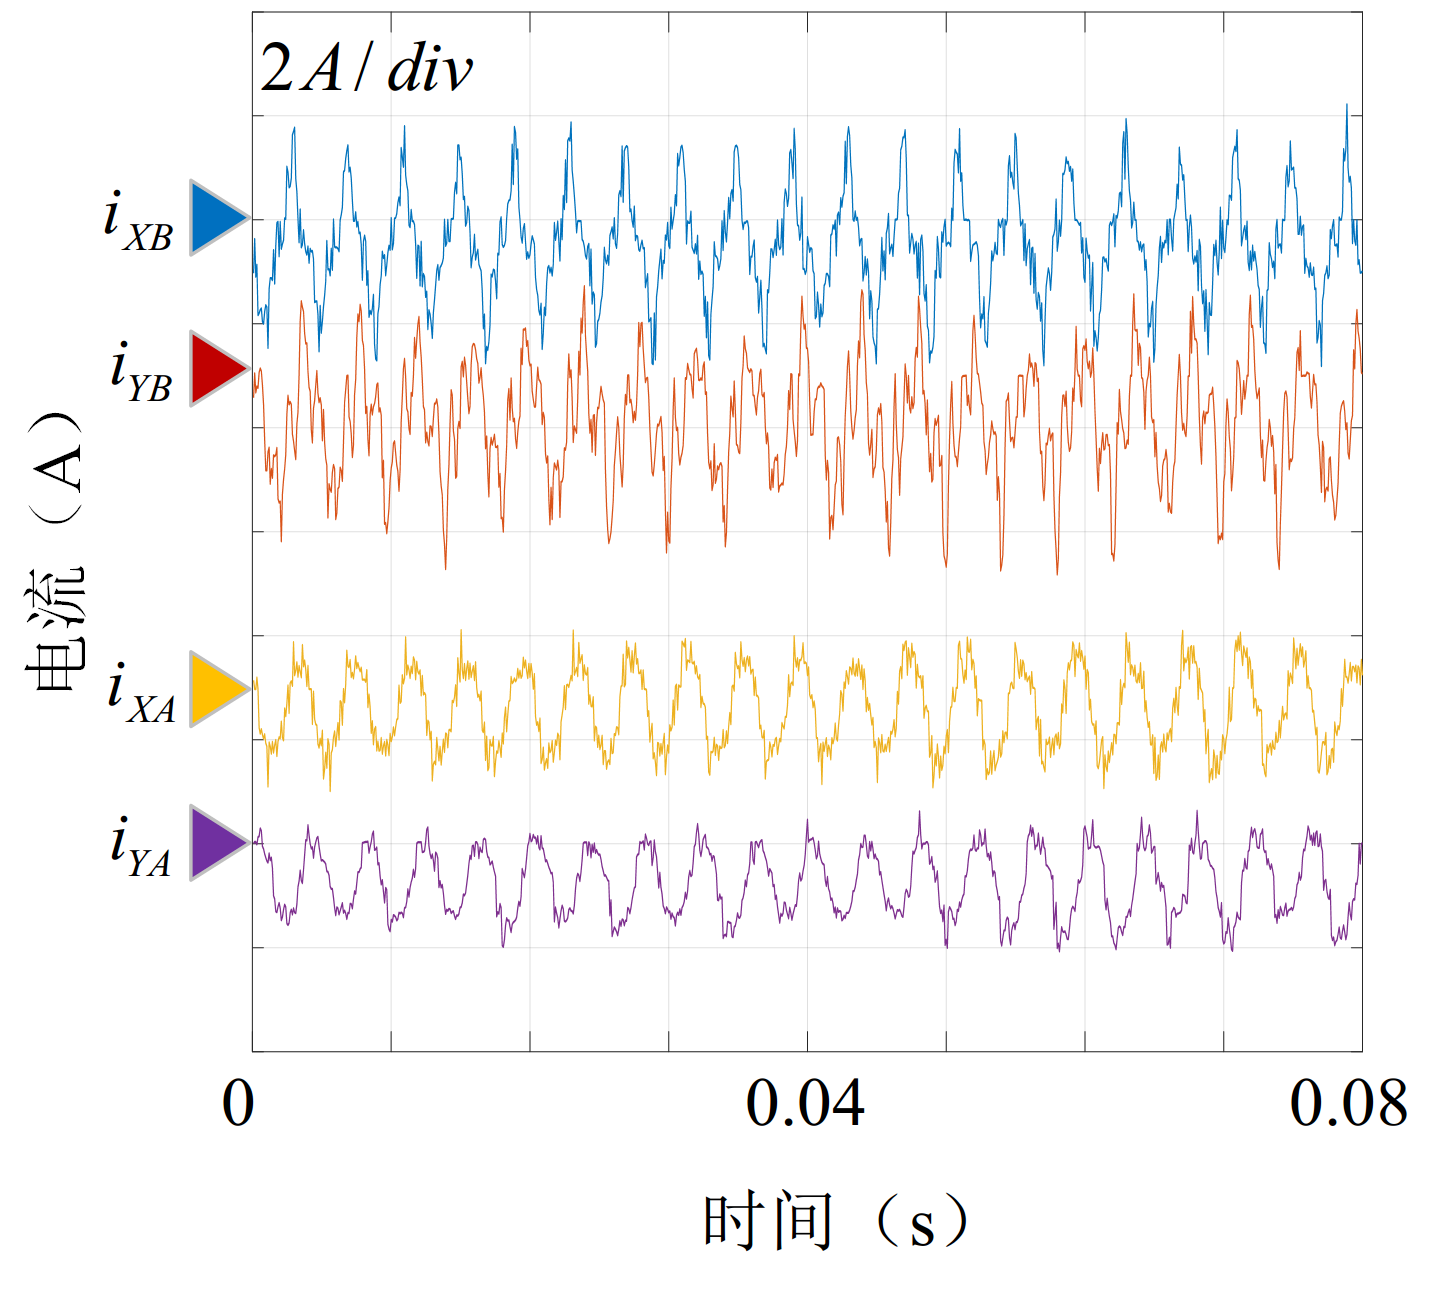
\includegraphics[scale=1.0]{5-s3-i-w1-pid.png}}\quad  
	\subfloat[现场动平衡前PID+重复控制器控制下线圈电流时域波形\label{fig:5-s3-i-w1-pid-orc}]{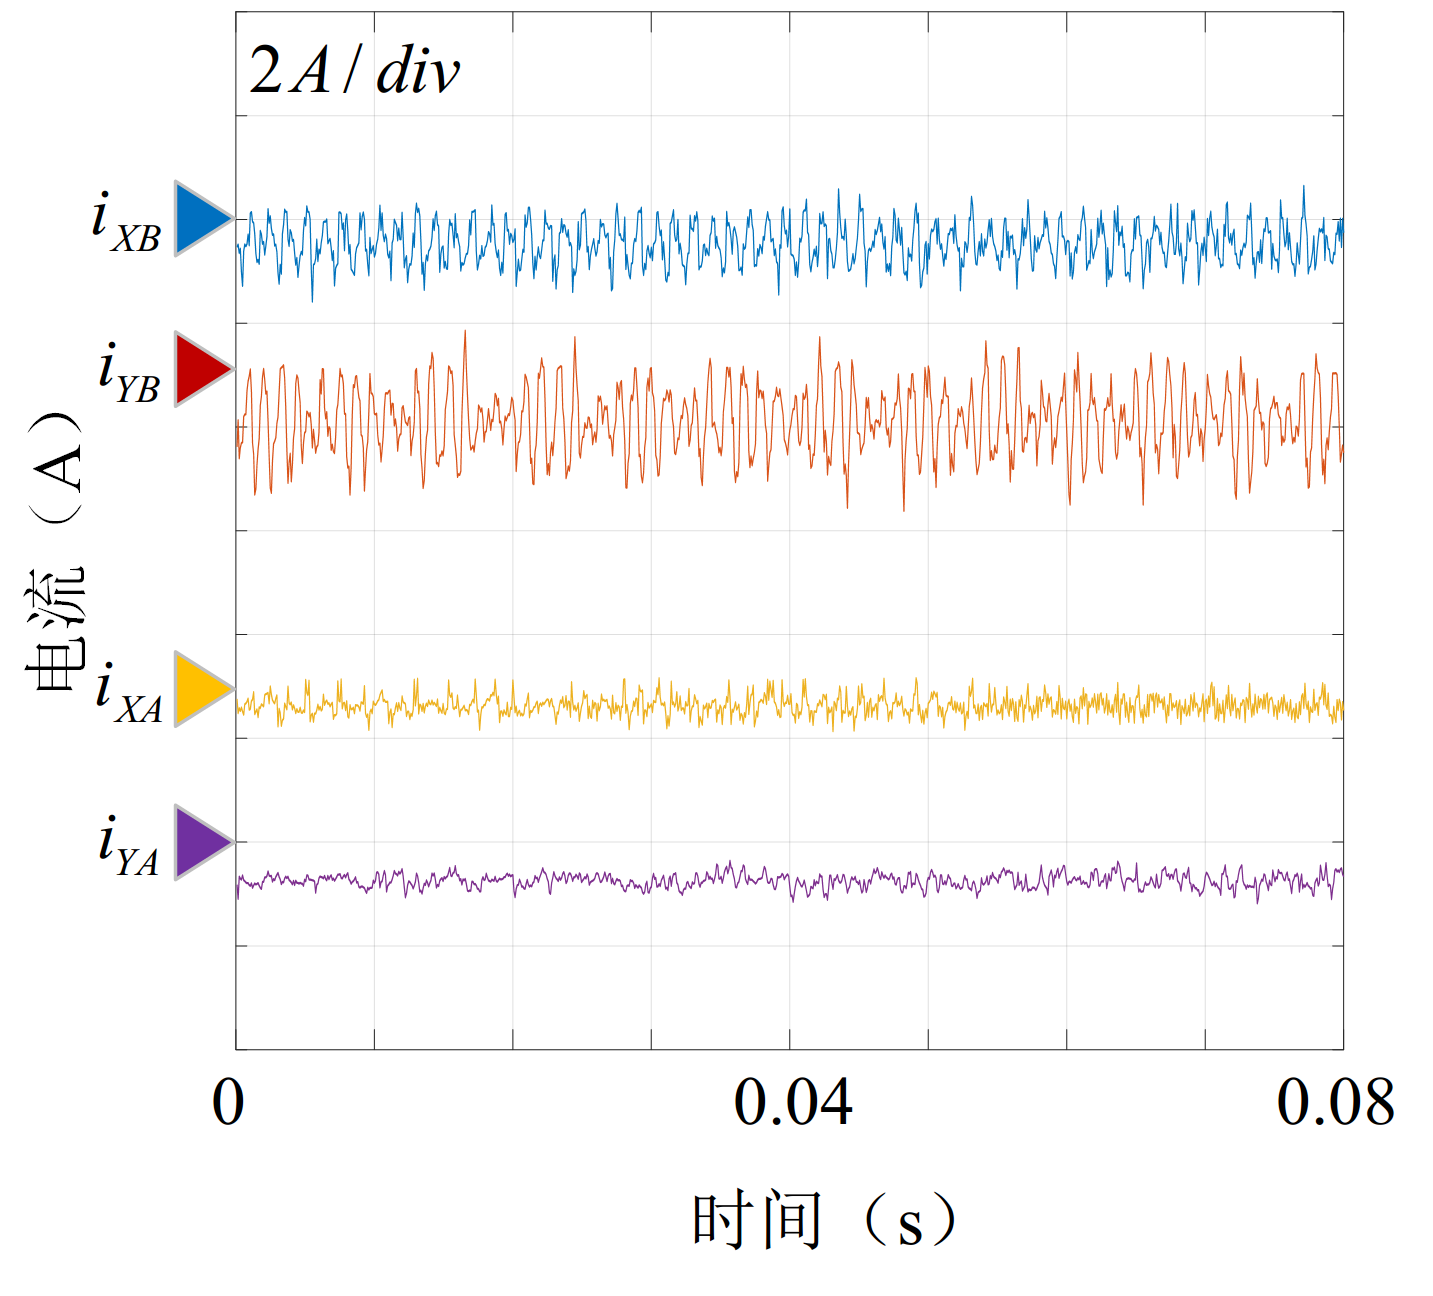
\includegraphics[scale=1.0]{5-s3-i-w1-pid-nf.png}}  
	\caption{现场动平衡前加入重复控制器前后线圈电流时域波形}  \label{fig:5-s3-i-w1-pid_orc}
\end{figure}

\begin{figure}
	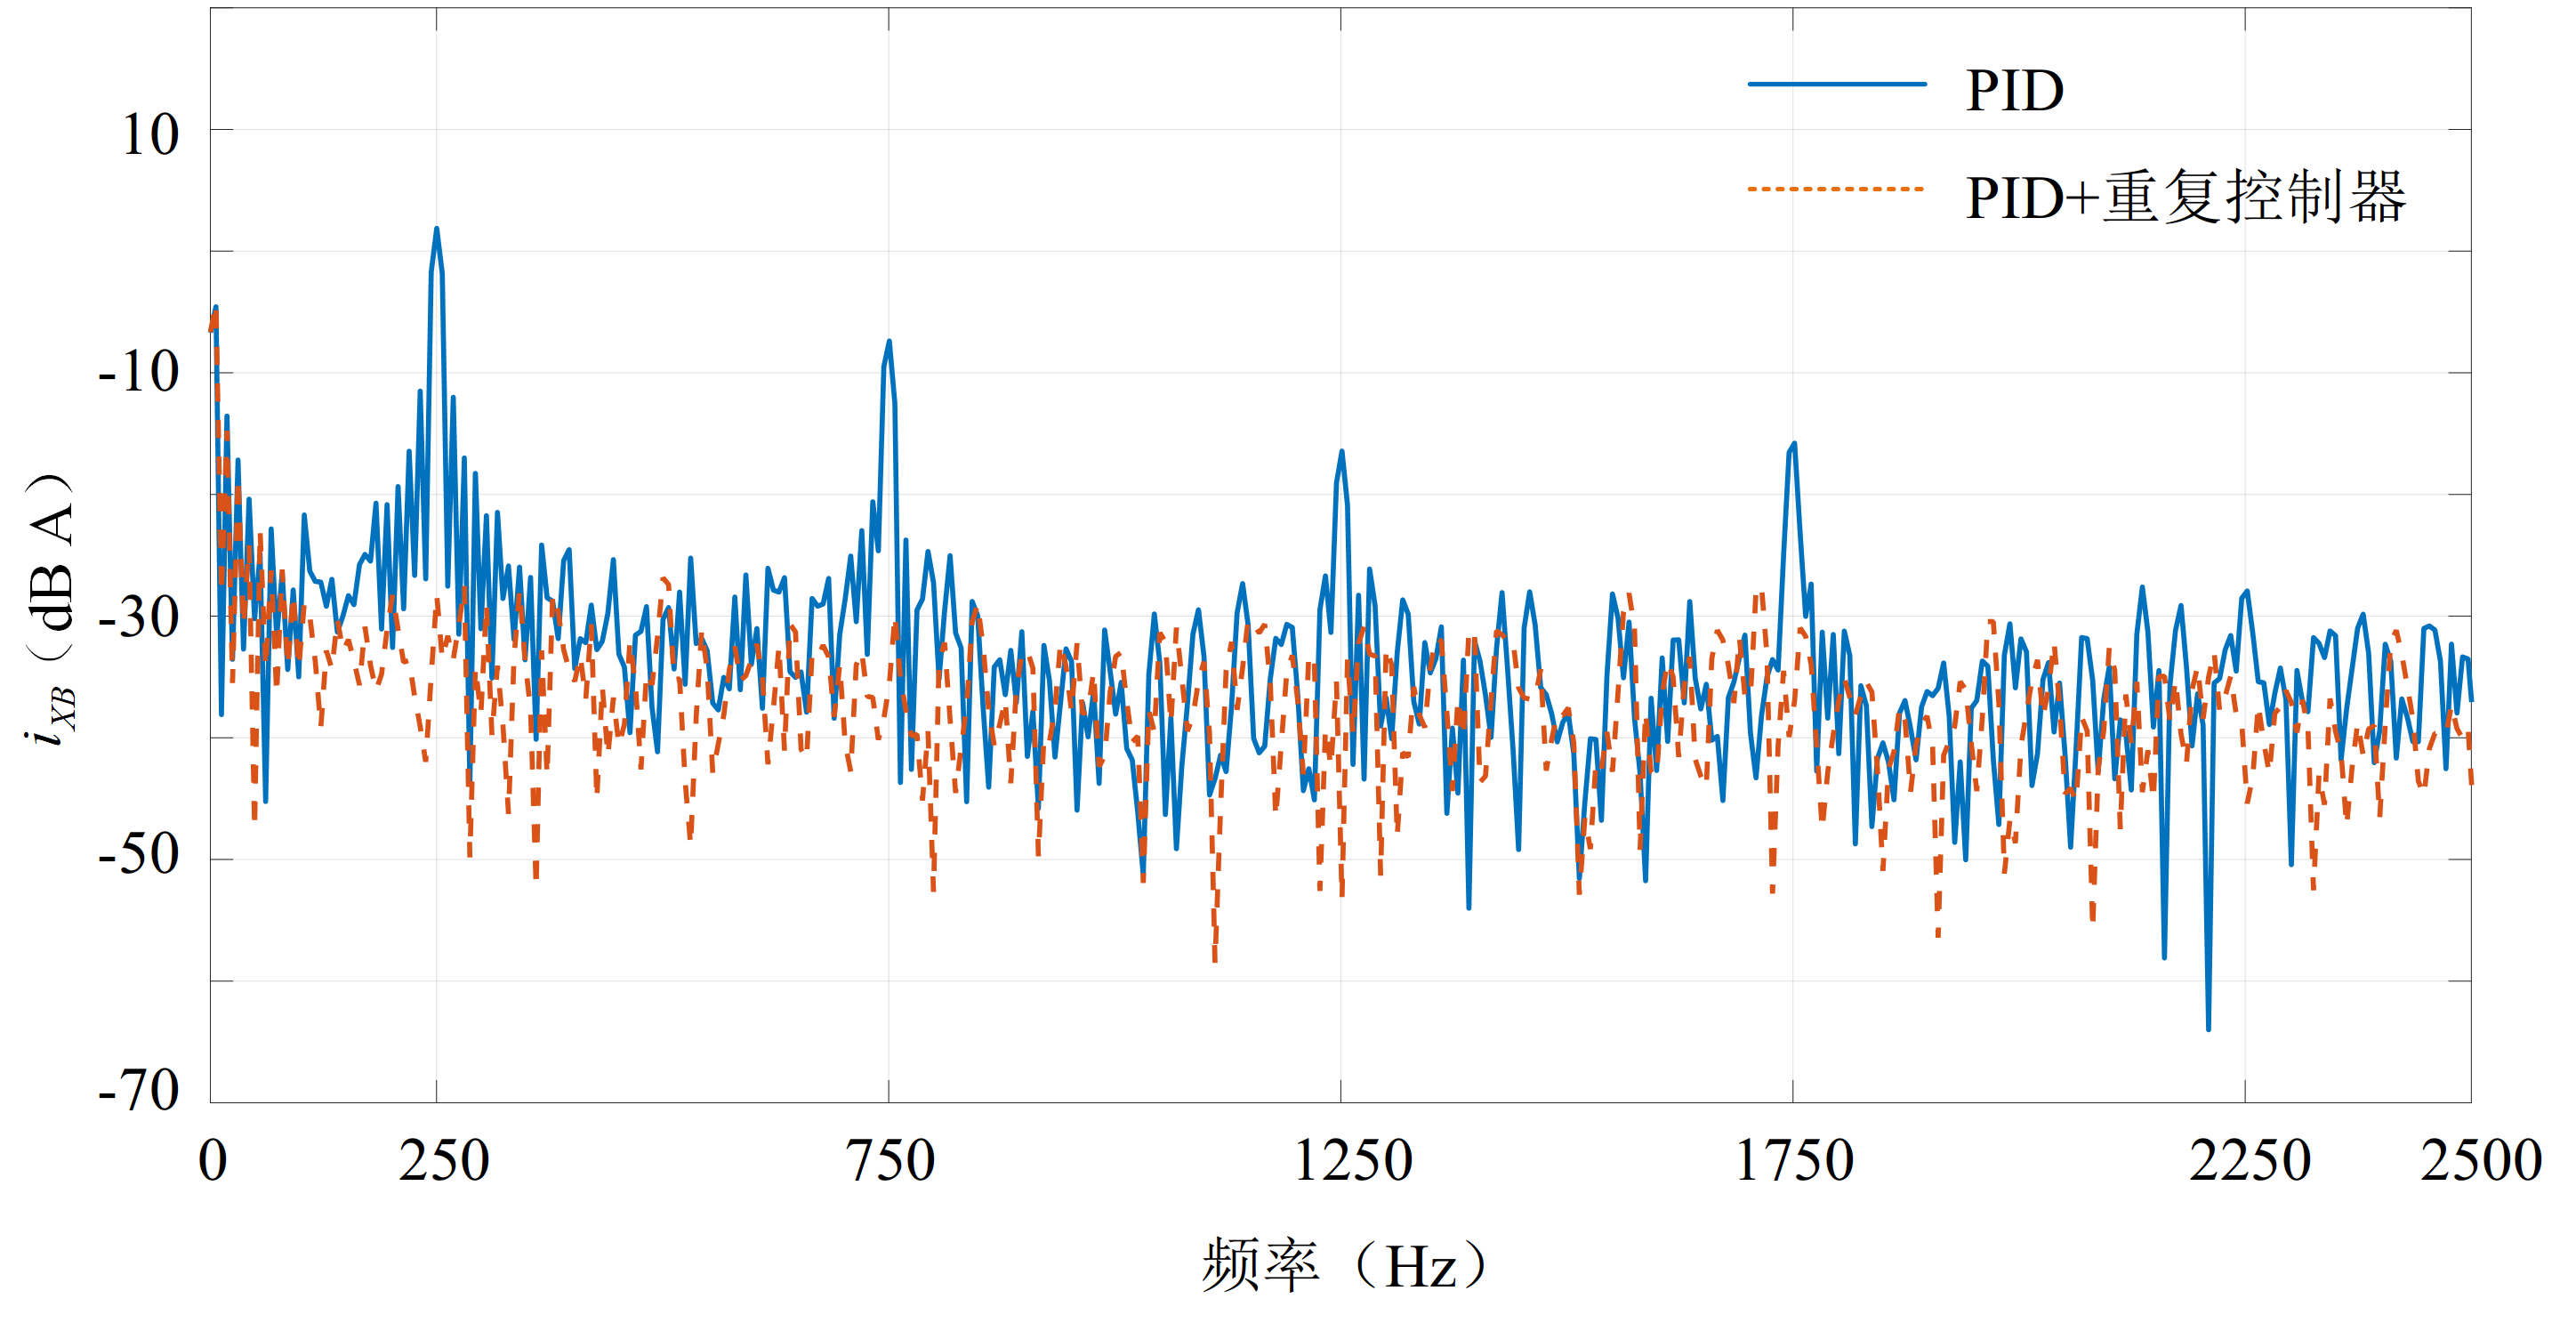
\includegraphics[scale=1.0]{5-s3-i_f-w1-pid_orc.png}
	\caption{现场动平衡前加入重复控制器前后$i_{sB}$频谱}
	\label{fig:5-s3-i_f-w1-pid_orc}
\end{figure}

\begin{figure}[htb]  
	\subfloat[现场动平衡前加入重复控制器前后B端转子轴心轨迹\label{fig:5-s3-x_locus-w1-pid-orc_bend}]{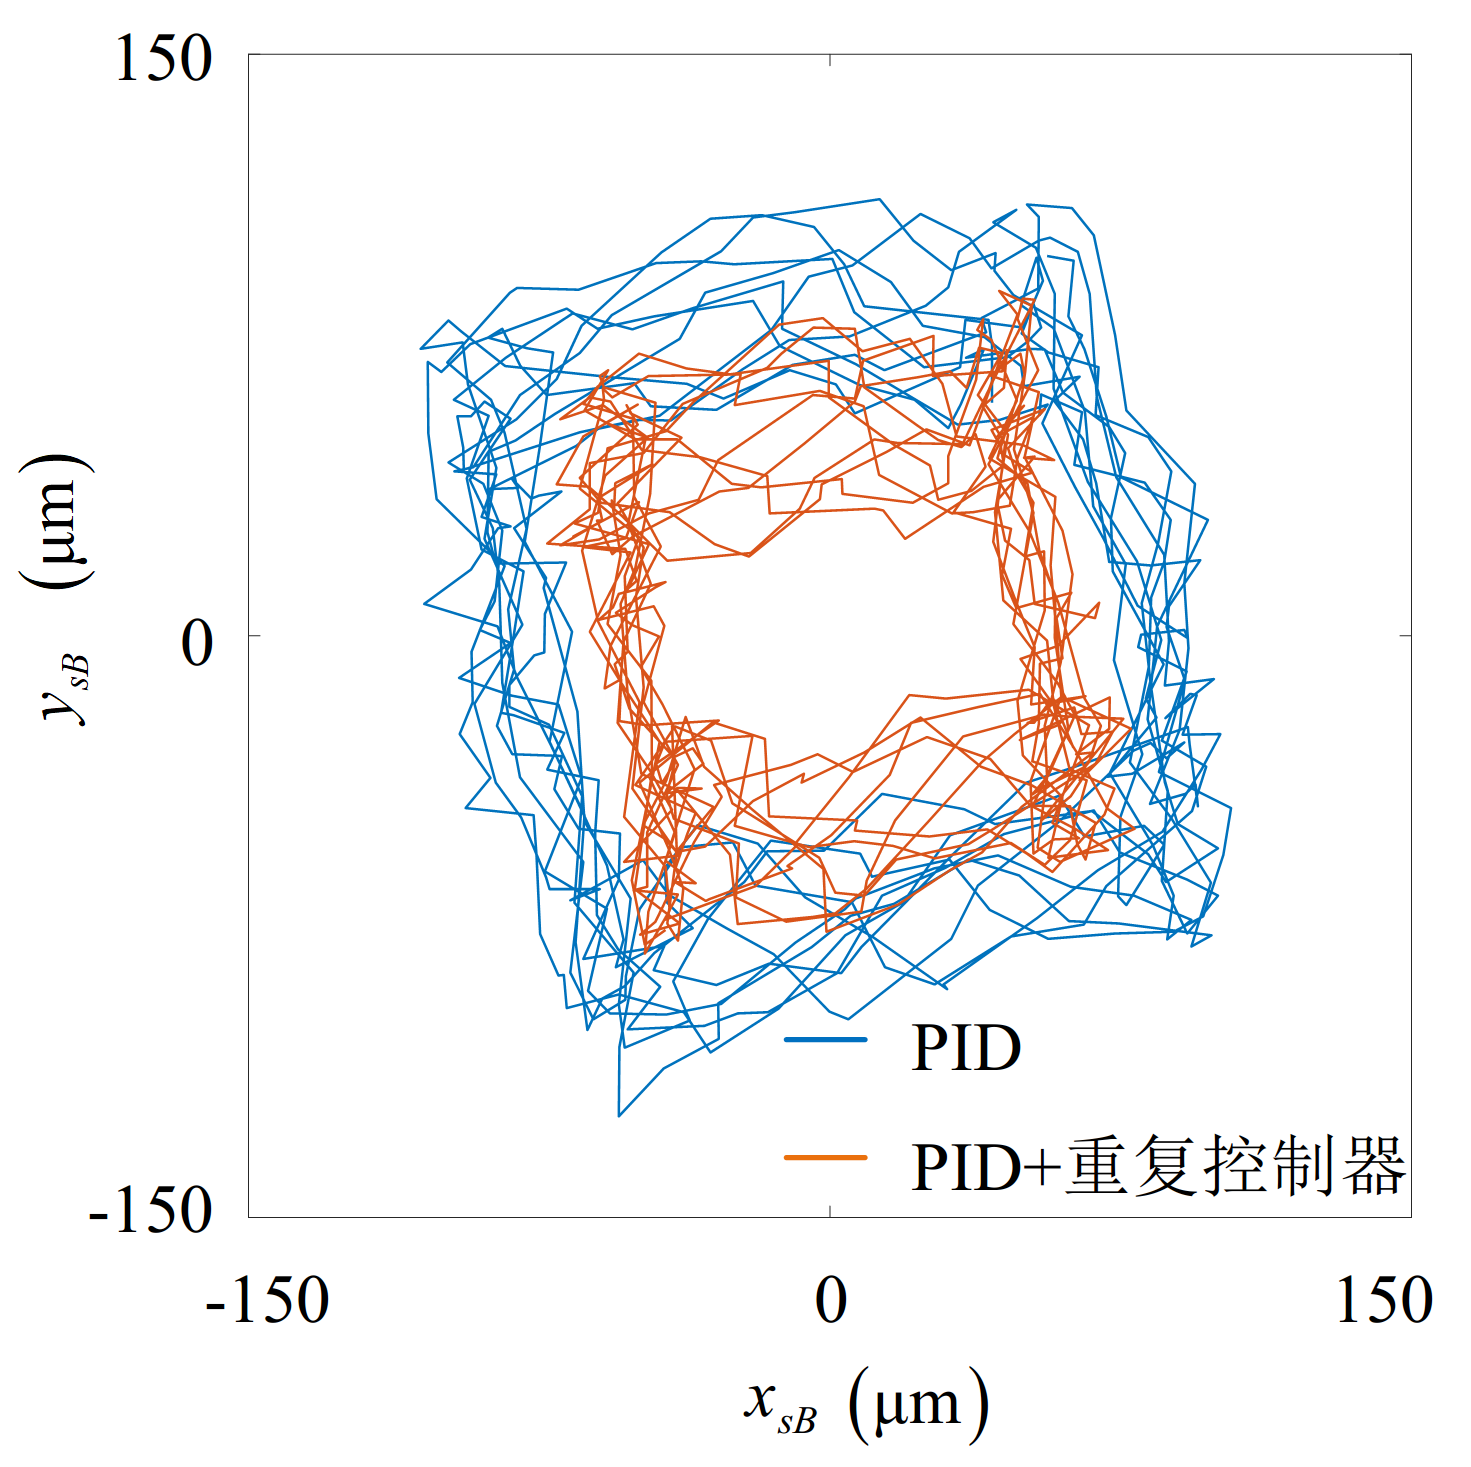
\includegraphics[scale=1.0]{5-s3-x_locus-w1-pid-orc_bend.png}}\quad  
	\subfloat[现场动平衡前加入重复控制器前后A端转子轴心轨迹\label{fig:5-s3-x_locus-w1-pid-orc_aend}]{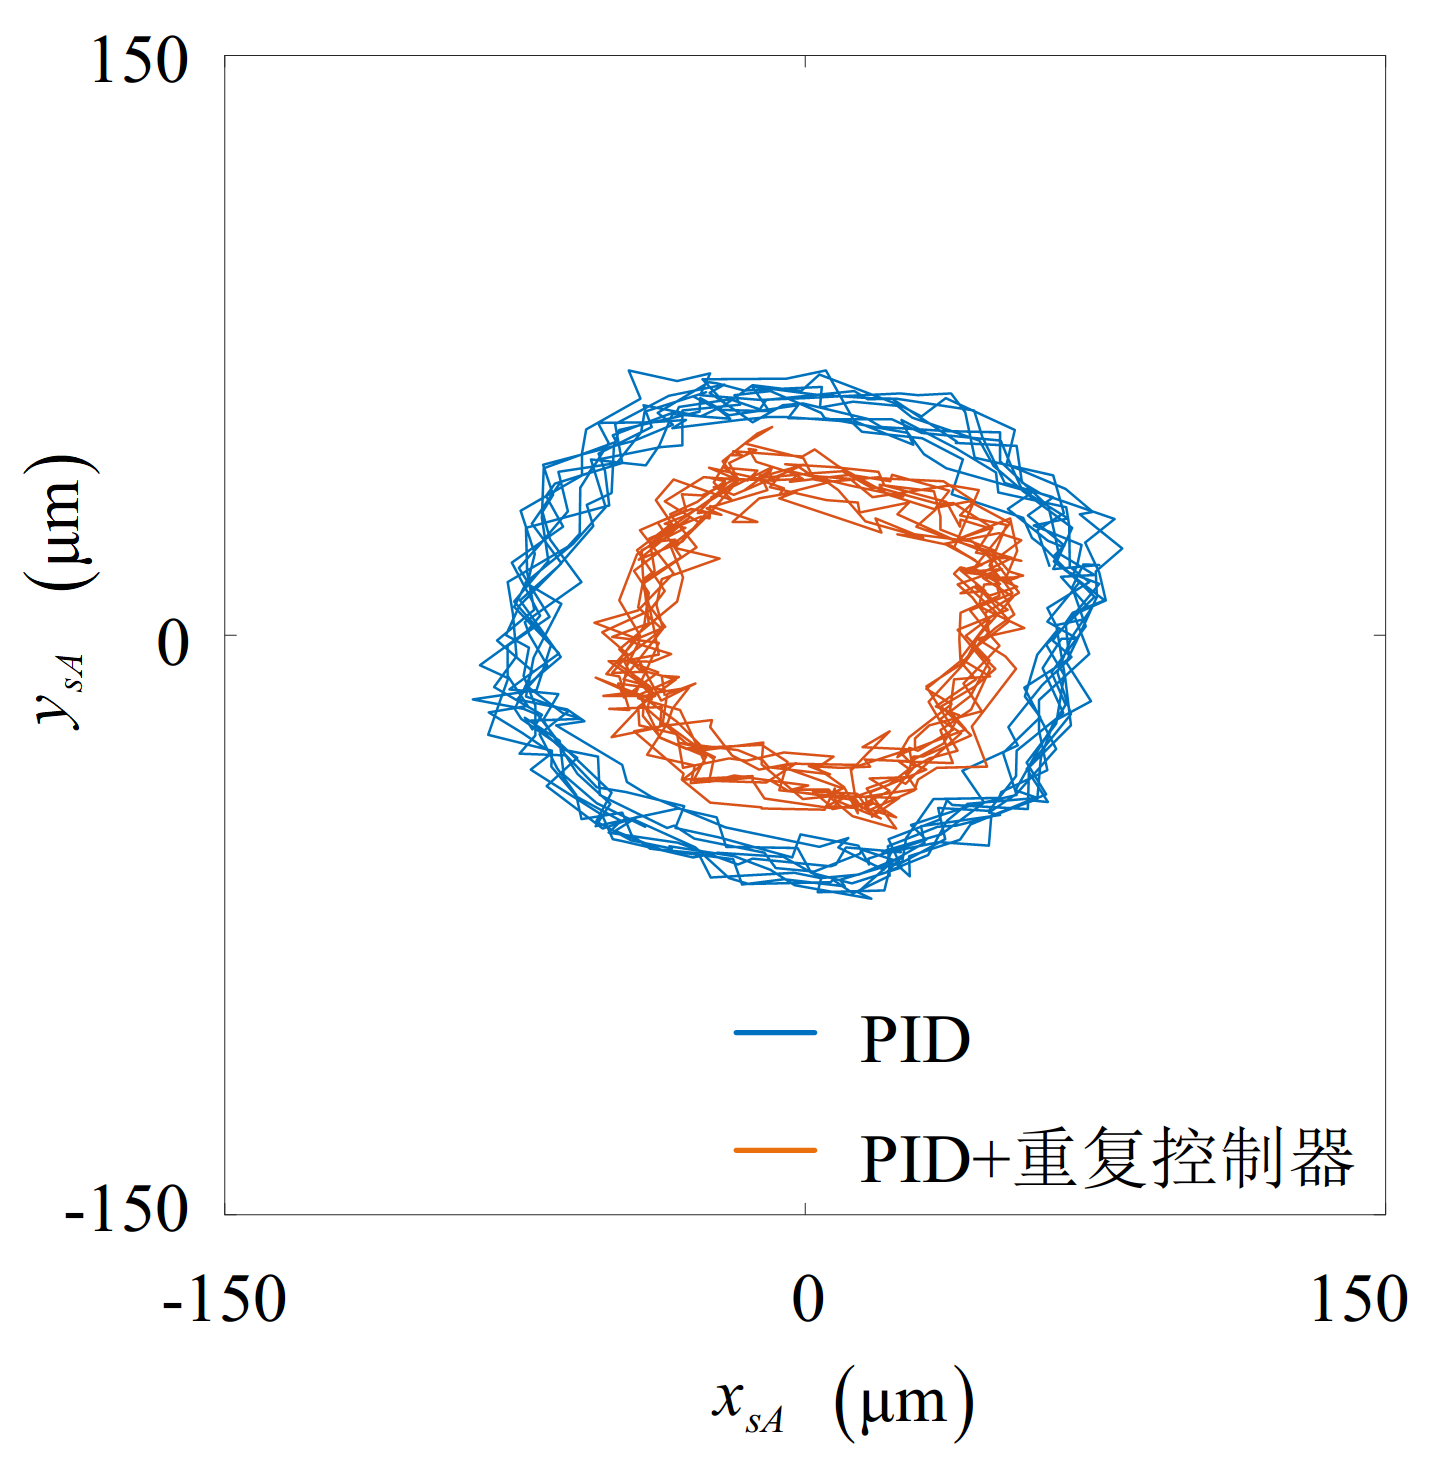
\includegraphics[scale=1.0]{5-s3-x_locus-w1-pid-orc_aend.png}}  
	\caption{现场动平衡前加入重复控制器前后转子双端轴心轨迹}  \label{fig:5-s3-x_locus-w1-pid-orc_end}
\end{figure}

\autoref{fig:5-s3-x_locus-w1-pid-orc_end}显示了现场动平衡前加入重复控制器前后转子双端轴心轨迹。其中\autoref{fig:5-s3-x_locus-w1-pid-orc_bend}所显示的轴心轨迹并不是较为规则的圆形,这是因为位移中含有的谐波成分较为丰富;与之对比的是\autoref{5-s3-x_locus-w1-pid-orc_aend}所示的轴心轨迹,因为位移谐波成分相对较少所以更接近圆形。可以看出加入重复控制器后,转子双端的轴心轨迹均呈现汇聚的趋势,表明转子振动量级显著降低,旋转轴趋近于惯性轴。


\subsection{辨识不平衡质量}

通过本章前文描述的自编的数据采集软件采集转角离散信号和四路位移离散信号。其采样频率为12.5kHz、长度为1000。根据第四章阐述的不平衡质量辨识方法,得到传统零电流控制方案和新型零电流控制方案下辨识出的不平衡质量大小和相位如\autoref{tab:nf_orc_w1}所示。

\begin{table}[htb]
  \caption[现场动平衡初始配重及辨识质量]{现场动平衡初始配重及辨识质量\label{tab:nf_orc_w1}}
\begin{tabular}{ccc}
    \toprule
    	项目  & 轴端 & 大小和相位 \\
    \midrule
		\multirow{2}{*}{初始配重质量}   
		& A  & $596mg \angle -140^{\circ}$      \\
		& B  & $559mg \angle -125^{\circ}$      \\    
		\multirow{2}{*}{陷波器法辨识的不平衡质量}   
		& A  & $660mg \angle -145^{\circ}$      \\
		& B  & $657mg \angle -125^{\circ}$      \\
		\multirow{2}{*}{重复控制器法辨识的不平衡质量} 
		& A  & $648mg \angle -148^{\circ}$      \\
        & B  & $646mg \angle -128^{\circ}$     	\\
		\multirow{2}{*}{实际校正质量(增重)} 
		& A  & $659mg \angle 35^{\circ}$      \\
        & B  & $654mg \angle 55^{\circ}$     	\\        
    \bottomrule
\end{tabular}
\end{table}

从\autoref{tab:nf_orc_w1}可以看出,基于陷波器法和基于重复控制器法辨识得到的不平衡质量大小与初始配重质量相比均偏大,解析得到的相位等于或略小于初始配重质量。由于除初始配重质量外,转子自身存在一定的不平衡质量分布,而该不平衡质量量级较小、分布无法准确测得,且可能导致实际的不平衡质量分布与初始配重质量发生一定偏差。此外,配重盘上的用于固定配重螺丝的螺纹孔分布间隔为$10^{\circ}$,相位读数无法精确到$10^{\circ}$。综合以上原因考虑此表显示的两种方案的辨识结果,仅可得出结论:陷波器法辨识的不平衡质量和重复控制器法辨识的不平衡质量精度基本一致。

\subsection{补偿不平衡质量}

根据第四章阐述的校正质量计算原理,计算得到的校正质量的大小与辨识的不平衡质量的大小相等,相位相差$180^{\circ}$。实际进行现场动平衡操作时,增重通过螺丝加垫片实现,这种方式无法做到连续的质量变化。间隔分布的螺丝孔使得增重的相位无法做到连续变化。因此实际增重质量与计算校正质量不是严格相等。本实验中的实际增重质量取计算校正质量的附近值,如\autoref{tab:nf_orc_w1}所示。

\begin{figure}
	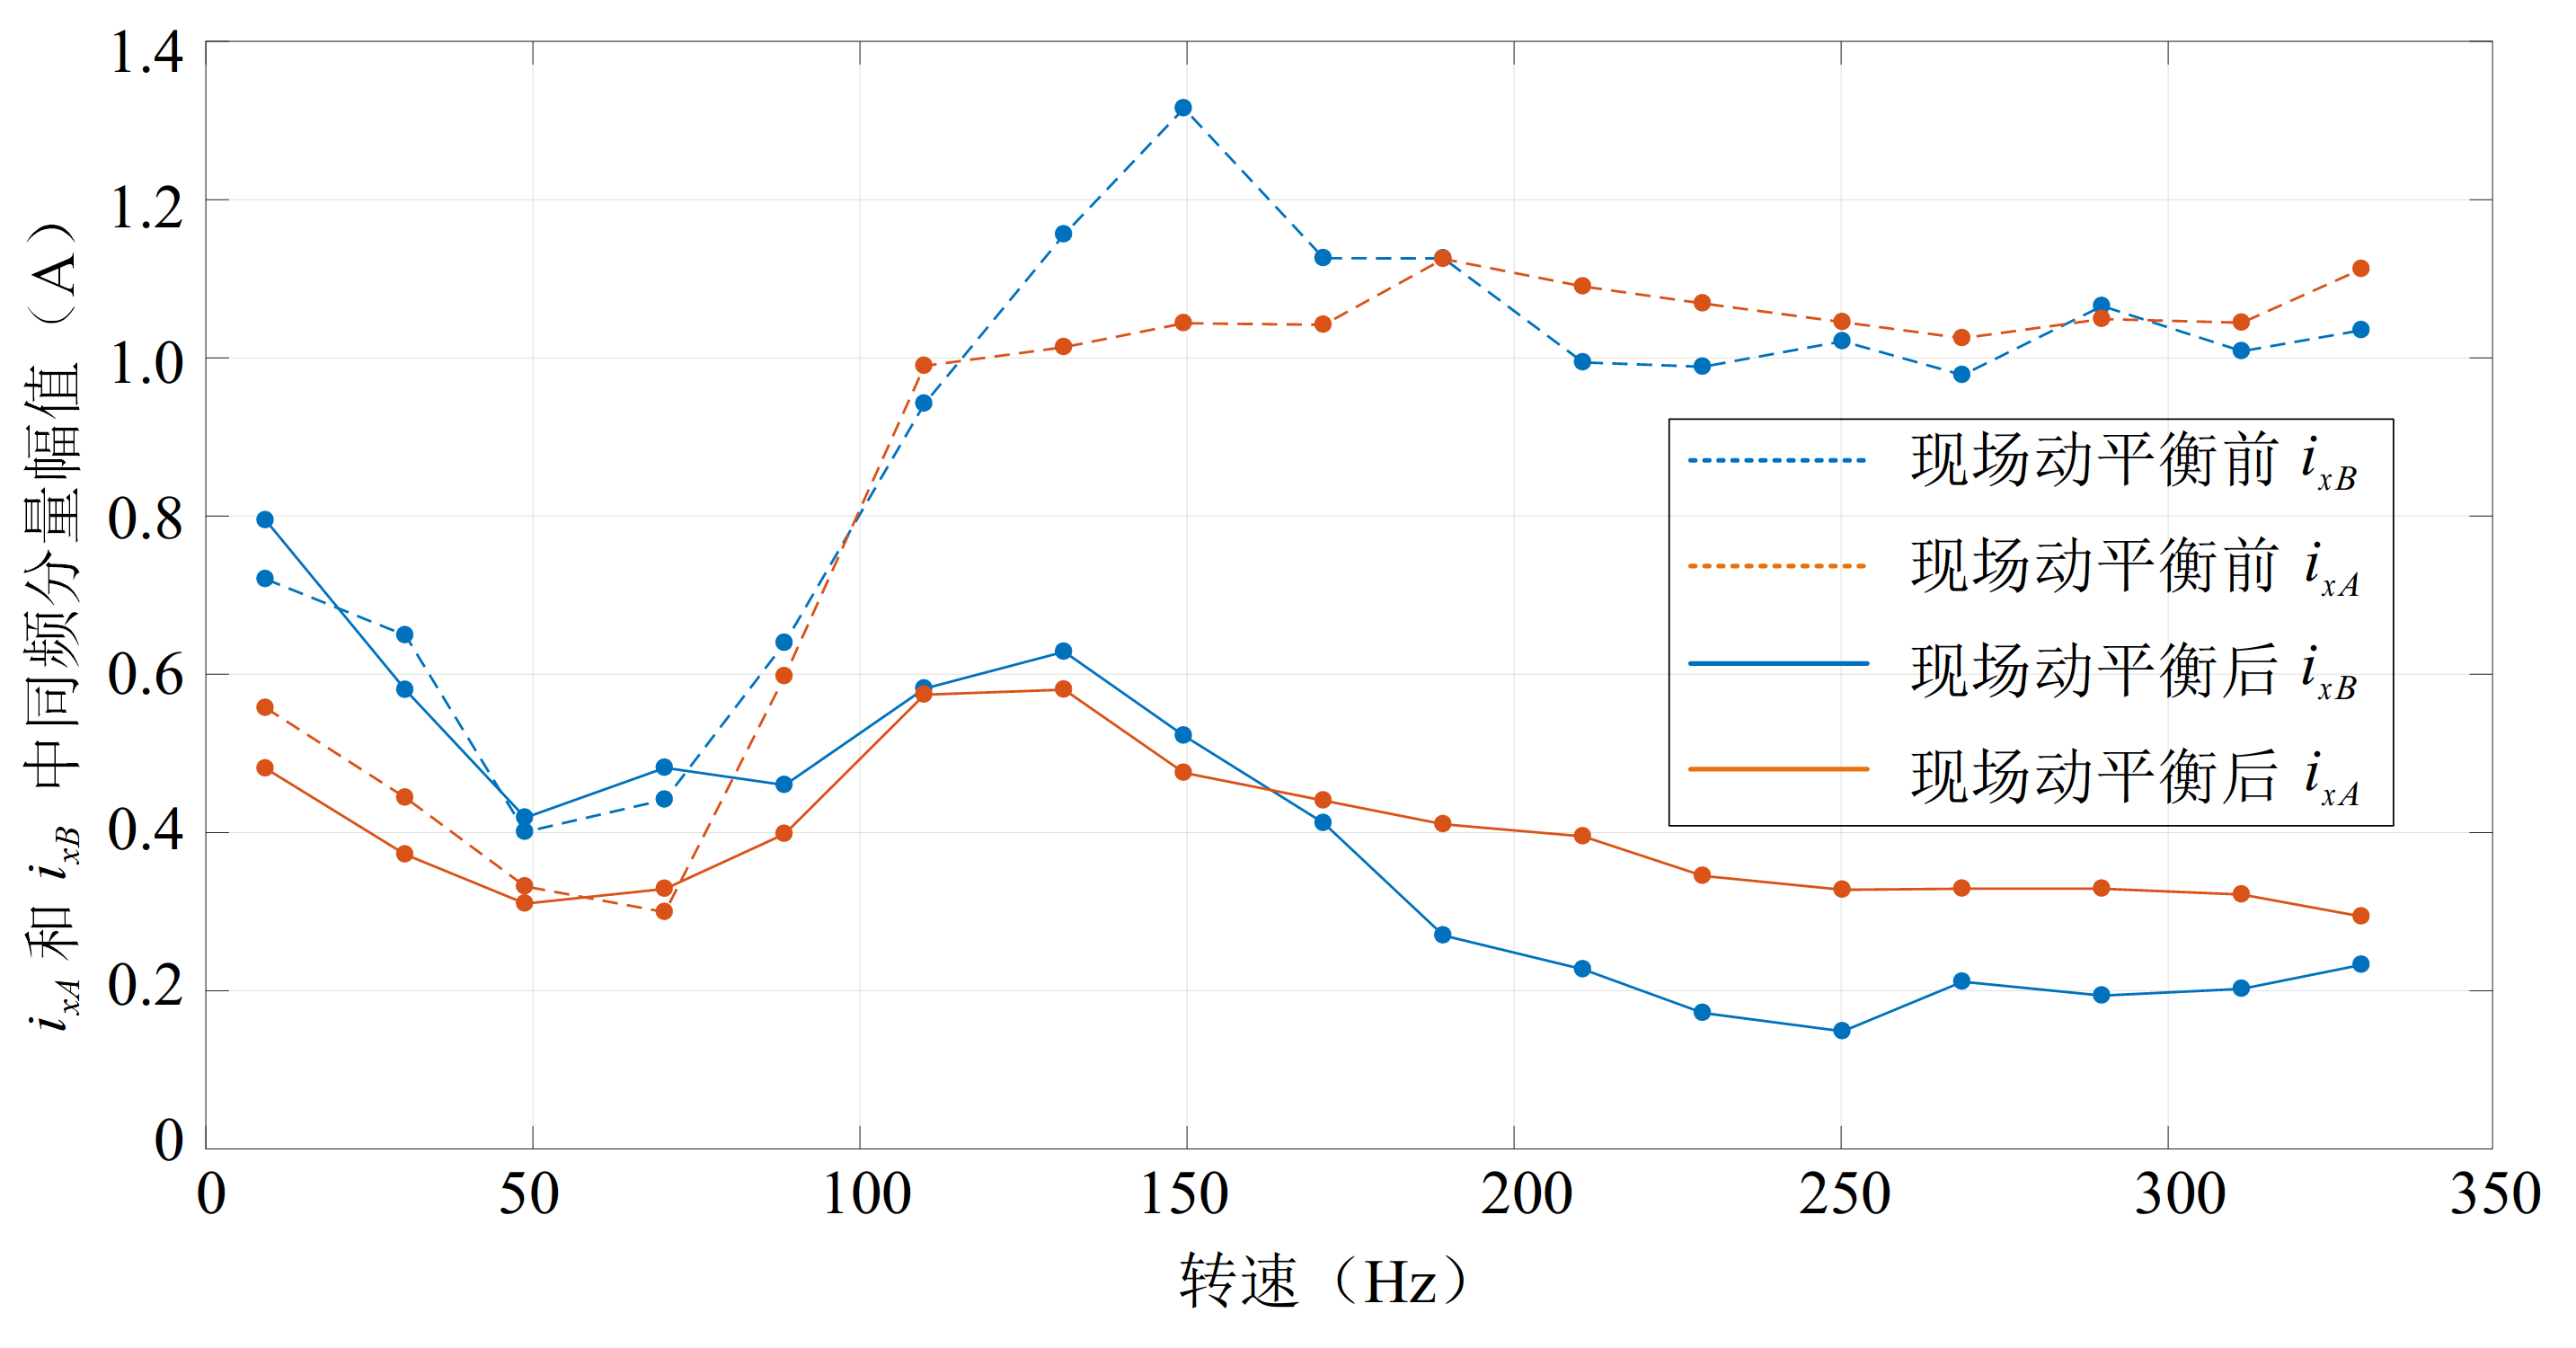
\includegraphics[scale=1.0]{5-s3-i-w1w2.png}
	\caption{现场动平衡前后$i_{xB}$、$i_{xA}$同频分量幅值}
	\label{fig:5-s3-i-w1w2}
\end{figure}

\autoref{fig:5-s3-i-w1w2}显示了现场动平衡前后控制电流中同频分量幅值。从图中可以看到,现场动平衡之前,A端磁轴承和B端磁轴承中的控制电流$i_{xA}$和$i_{xB}$中的同频分量的幅值随着转速变化而变化,从10Hz处的0.7A附近先下降到约0.4A,然后上升到约1.1A,之后稳定在1.1A附近。完成现场动平衡之后,在90Hz前$i_{xA}$和$i_{xB}$中的同频分量的幅值与现场动平衡之前没有显著的变化,在90Hz之后,随着转速继续升高,二者则始终比现场动平衡之前的值小得多,稳定在约0.3A附近。

\begin{figure}
	\includegraphics[scale=1.0]{5-s3-x-w1w2.png}
	\caption{现场动平衡前后$x_{sB}$、$x_{sA}$同频分量幅值}
	\label{fig:5-s3-x-w1w2}
\end{figure}

\autoref{fig:5-s3-x-w1w2}显示了现场动平衡前后转子轴端位移中同频分量幅值。从图中可以看到,现场动平衡之前,A端磁轴承和B端磁轴承中的位移$x_{sA}$和$x_{sB}$中的同频分量的幅值随着转速变化而变化,二者先从10Hz处约$80 \mu m$和$120 \mu m$处先下降再上升到约$70\mu m$,最后下降稳定到约$30 \mu m$;现场动平衡之后,90Hz前$x_{sA}$和$x_{sB}$与现场动平衡之前无显著区别。90Hz后,$x_{sA}$和$x_{sB}$中的同频分量幅值始终小于现场动平衡之前的幅值,最终稳定在约$10 \mu m$处。\autoref{fig:5-s3-i-w1w2}和\autoref{fig:5-s3-x-w1w2}所示的实验现象说明本文采取的基于重复控制器的现场动平衡方法有明显振动抑制效果。

\section{本章小结}

\chapter{总结与展望}
\section{研究内容总结}
\section{下一步工作展望}